\documentclass[letterpaper, 10 pt, conference]{ieeeconf}  % Comment this line out if you need a4paper
%\documentclass[a4paper, 10pt, conference]{ieeeconf}      % Use this line for a4 paper
\IEEEoverridecommandlockouts                              % This command is only needed if 
\overrideIEEEmargins                                      % Needed to meet printer requirements.

\usepackage{graphics} % for pdf, bitmapped graphics files
\usepackage{pgf,lmodern}
\usepackage{amsmath,amssymb}  % assumes amsmath package installed
\usepackage{cite}
\renewcommand{\d}{\mathrm{d}}
\def\mathdefault#1{#1}
\title{\LARGE \bf
Using a Neural Network Trained Only on Integer Order Systems to Identify
Fractional Order Dynamics in Large Scale Systems}


\author{Bill Goodwine$^{1}$ and Tan Chen$^{2}$% <-this % stops a space
\thanks{$^{1}$Bill Goodwine is with the Department of Aerospace \& Mechanical
  Engineering, University of Notre Dame, Notre Dame, IN 46556, USA
{\tt\small billgoodwine@nd.edu}}%
\thanks{$^{2}$Tan Chen is with the Department of Electrical and Computer
Engineering, Michigan Technological University, Houghton, MI 49931, USA
{\tt\small tanchen@mtu.edu}}
}
\begin{document}
\maketitle
\thispagestyle{empty}
\pagestyle{empty}

\begin{abstract}

  This paper presents a standard feed forward artificial neural network that
  identifies the order of the dynamics of a unit step response. The main
  contribution of this paper is the demonstration that a system that is trained
  on only integer order, first and second order systems, can identify fractional
  order responses with a high degree of accuracy. The details of the design of
  structure of the neural network, the training method and the training sets, as
  well as statistics describing the accuracy of the fractional predictions are
  presented. Also using the neural network to identify fractional dynamics for a
  large scale networked system from the authors' prior work is presented as
  further validation and a demonstration of the applicability of the results.
  This demonstrates the potential for practicing engineers to use similar
  machine learning tools trained on ``standard'' systems with the ability to
  distinguish when features such as fractional order dynamics are significant
  and warrant deeper consideration for the design or control of such a system. 

\end{abstract}


\section{INTRODUCTION}

  \begin{figure}
  \centering
  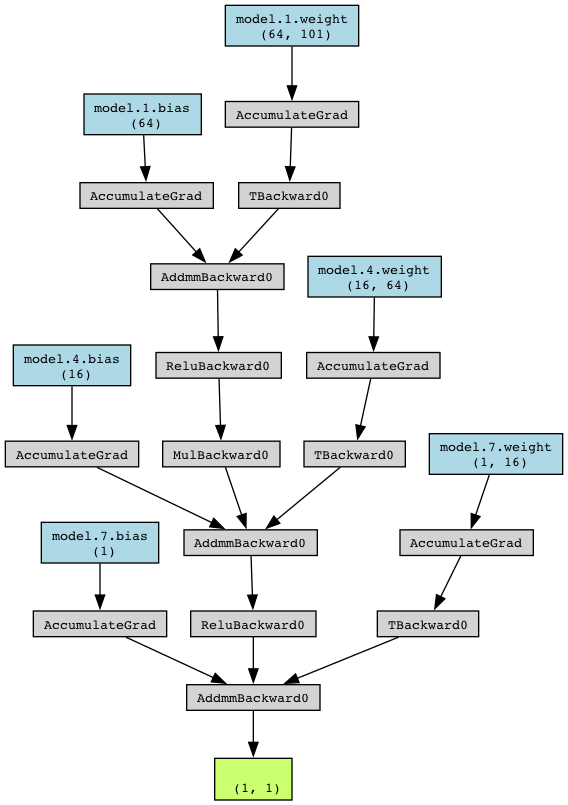
\includegraphics[width=3.5in]{viz.png}
  \caption{The neural network.}
  \label{fig:thennet}
  \end{figure}


  Fractional calculus and fractional order dynamics are increasingly important
  in modern engineered systems. Unlike integer order derivatives, fractional
  order derivatives, and hence the dynamics that depend on them, are
  \emph{nonlocal}. As such, many modern, large scale engineered systems may
  exhibit fractional order dynamics and responses because interactions among
  various components in the system may be significantly displaced in time or
  space. In instances where significant fractional order dynamics are present,
  control algorithms which directly address the fractional nature of the system
  may be superior.  Therefore, tools to readily identify if significant
  fractional order dynamics are present are needed.

  There is a vast literature on fractional calculus. Some textbooks include
  \cite{fracbook,fracbook2,oustaloup}.  Fractional-order control is considered
  in many topical areas, but particularly relevant to this paper is fractional
  order controls, such as in \cite{fraccontrol,YQChenAcc}. An excellent review
  article illustrating the very broad range of applications of fractional
  calculus and control in science and engineering is \cite{SUN2018213}.


  Our main interest are identifying cases where fractional order models may
  provide useful ``reduced order'' models for large scale systems
  \cite{goodwinemed2023,goodwinemmar2023} and for exact models for many large
  scale systems
  \cite{Goodwine2014Modeling,Leyden2016Using,Leyden2019Large,bg:xnids2022,bg:xninonlinear2020}.
  A fractional order system is arguably infinite order, but a fractional order
  representation is more concise than, for example, an extremely high order
  system like those considered in the preceding references.  While this paper
  does not build upon it, our closest publication to this would be
  \cite{bg:chenSII2022} where we created a symmetric neural network with a
  sequential set of identical layers. When it was trained on first derivatives
  of functions, the middle layer could represent the half derivative. 
 
 There are many different definitions of the fractional derivative. As will be
 outlined in the next section, a common feature of these is replacing factorial
 functions appearing in many integer-order representations of the derivative
 with gamma functions. The Riemann-Liouville, Caputo and the Gr\"unwald-Letnikov
 definitions are perhaps the most common examples of fractional derivative
 definitions, and the reader is referred to the references
 \cite{Machado20111140,4609961,series/lnee/Ortigueira11,das2011functional} for
 descriptions and definitions of each. Because of the python library we utilize
 for this paper, the definition used herein is the Caputo fractional derivative. 

 Machine learning in general and neural networks in particular have a long
 history. One of the earliest works related to the feed forward neural network,
 the type used in this paper, is from 1960 by Rosenblatt \cite{Rosenblatt1960}.
 In the 1970s, advanced in training by the back propagation method were
 developed \cite{linnainmaa1} and were further advanced in the 1980s
 \cite{werbos}.  Additionally in the 1980s theoretical advances such as the
 universal approximation theorem \cite{hornik1989multilayer} were developed.
 These practical advances buttressed with theoretical support helped advance the
 cause for usefulness of artificial neural networks. Of course, the confluence
 of ubiquitous data and advanced in computer processing power enabled many
 applications in the beginning of the 21st century has resulted in the rapid
 deployment throughout many aspects of modern life. 
 

 The rest of this paper is organized as follows. Section~\ref{sec:fractional}
 provides a limited introduction to fractional calculus, including the concepts
 needed for this paper. Section~\ref{sec:network} presents the details of the
 artificial neural network used and the integer order training data.
 Section~\ref{sec:generalize} presents the results when the neural network is
 used to identify fractional order dynamics. Section~\ref{sec:scalefree}
 further validates the results by applying the network to identify fractional
 order dynamics in a large scale networked system from the literature. Finally,
 Section~\ref{sec:conclusions} presents the conclusions and an outline of
 ongoing and future work. 

\section{FRACTIONAL CALCULUS}
\label{sec:fractional}

  This section gives a very brief overview of only the fractional calculus
  topics necessary to implement the methods in this paper and is therefore
  incomplete. The interested reader is referred to the references above for a
  complete exposition.

  The obvious task for fractional calculus is to define derivatives ``in
  between'' the usual integer order derivatives, \textit{e.g.}, 
\[
x(t) = \frac{\d^0 x}{\d t^0}(t), \quad\frac{\d^{1/2} x}{\d
t^{1/2}}(t), \quad \frac{\d x}{\d t}(t),  \quad \frac{\d^{5/4} x}{\d
t^{5/4}}(t), \ldots.
\]
  For one approach to generalizing the derivative to real, possibly noninteger,
  orders, consider the first and second order backwards finite difference
  equations for $\Delta t \ll 1$
\[
 \frac{\d x}{\d t}\left(t\right) \approx \frac{x(t) - x \left(t - \Delta
 t\right)}{\Delta t}
 \]
 and
 \[
    \frac{\d^2 x}{\d t^2}\left(t\right) \approx \frac{x(t) - 2 x \left(t - \Delta
    t\right) + x(t - 2 \Delta t)}{\left( \Delta t \right)^2}.
 \]
 As is well known, from these two equations it is clear that the formula for an
 arbitrary positive integer order derivative is
 \begin{equation}
  \frac{\d^n x}{\d t^n}(t) \approx \frac{\sum_{i=0}^n \left( -1 \right)^i
  \left( \frac{n!}{i! \left( n - i \right)!} \right) x ( t - i \Delta t )}{\left( \Delta t
  \right)^n},
  \label{eq:finitediff}
 \end{equation}
 where the fraction that is the coefficient of $x(t - i \Delta t)$ with the
 factorials in the numerator and denominator is the binomial coefficient. Note
 that the number of terms in the sum is one more than the order of the
 derivative.  The only terms in Equation~\ref{eq:finitediff} that must be
 integers are the factorials. Because the gamma function can be considered a
 generalization of the factorial because $n! = \Gamma(n+1)$ for integer values
 of $n$, a generalized equation results with
 \begin{equation}
    \frac{\d^\alpha x}{\d t^\alpha}(t) \approx \frac{\sum_{i=0}^{\lceil
    \frac{t}{\Delta t} \rceil} \left( -1 \right)^i \left(
    \frac{\Gamma(\alpha+1)}{i! \Gamma\left( \alpha - i + 1\right)} \right) x ( t
    - i \Delta t )}{\left( \Delta t \right)^\alpha},
    \label{eq:gw}
 \end{equation}
 where the symbol for the order of the derivative was changed from $n$ to
 $\alpha$ to connote that it no longer must be an integer. 
 If, instead of $\Delta t \ll 0$ the limit as $\Delta t \rightarrow 0$ is used,
 this equation becomes the Gr\"unwald-Letnikov derivative (see the references
 cited in the introduction for a complete exposition). 
  
  The generalized binomial coefficient in Equation~\ref{eq:gw} is nonzero for
  all values of $i$ (except when $\alpha$ is an integer), and hence the sum
  will include times spanning all of history. In the controls context assuming
  zero initial conditions and zero values for all time prior to zero, the sum
  will include terms at all time steps between $0$ and the current $t$. This
  highlights an important distinction between integer order derivatives and
  fractional order derivatives, which is that the latter are \emph{nonlocal}.
  It also highlights the fact that computing fractional derivatives is
  computationally expensive compared to integer order derivatives. 

  The method to compute the fractional step responses that the neural network
  will identify was computed by a different method than what is expressed in
  Equation~\ref{eq:gw}, but is similar in spirit. Specifically, we use the
  \texttt{numfracpy} python library to numerically compute fractional step
  responses, and from its documentation\footnote{http://tinyurl.com/yyytpv8d} the step response is computed using a
  fractional order Adams predictor corrector method given by
  \begin{align*}
  x^P_{n+1} &= \sum_{j=0}^{m-1} \frac{t^j_{n+1}}{j!}x_0^j + \left( \Delta t
  \right)^\alpha \sum_{j=0}^n b_{j,n+1} f\left( t_j, x_j \right) \\
  x_{n+1} &=  \sum_{j=0}^{m-1} \frac{t^j_{n+1}}{j!}x_0^j + \sum_{j=0}^n \big[ a_{j,n+1}
  f \left( t_j, x_j \right) + \\ &\  \hspace*{1in} a_{n+1,n+1} f\left( t_{n+1},
x^P_{n+1} \right) \big]
  \end{align*}
  where
  \[
  b_{j,n+1} = \frac{1}{\Gamma (\alpha + 1 )} \left[(n-j+1)^\alpha -
  (n-j)^\alpha \right]
  \] and
  \[\alpha_{0,n+1} = \frac{\left(\Delta t \right)^\alpha \left[n^{\alpha + 1} -
  (n-\alpha)(n+1)^\alpha\right]}{\Gamma \left( \alpha + 2 \right)},
  \]
  \begin{multline*}
  a_{j,n+1} = \frac{\left( \Delta t \right)^\alpha}{\Gamma \left( \alpha + 2
  \right)} \big[ (n-j+2)^{\alpha + 1} \\
  -2 (n - j + 1)^{\alpha + 1} + (n-j)^{\alpha + 1} \big]
  \end{multline*} for $1 \leq j \leq n$
  and
  \[
  \alpha_{n+1,n+1} = \frac{\left( \Delta t \right)^\alpha}{\Gamma\left(\alpha +
  2\right)}.
  \]
  The summations in the expressions for $x_{n+1}$ are the parts of the
  expressions that include the nonlocal terms.

\section{Neural Network and Training}

  The neural network used in this paper is illustrated in
  Figure~\ref{fig:thennet}. There is an input layer with 101 nodes, a hidden
  layer with 64 nodes, a subsequent hidden layer with 16 nodes, another hidden
  layer with 16 nodes, and an output layer with 1 node. Each hidden layer has
  the ReLU activation function. The values input to the network is the unit step
  response of a linear system in the time range of $0 \leq t \leq 10$
  discretized into time steps of $\Delta t = 0.1$ [s], which gives 101 input
  nodes. The single output of the network is the order of the system that
  produced the input step response. 

  \begin{figure}
  \centering
  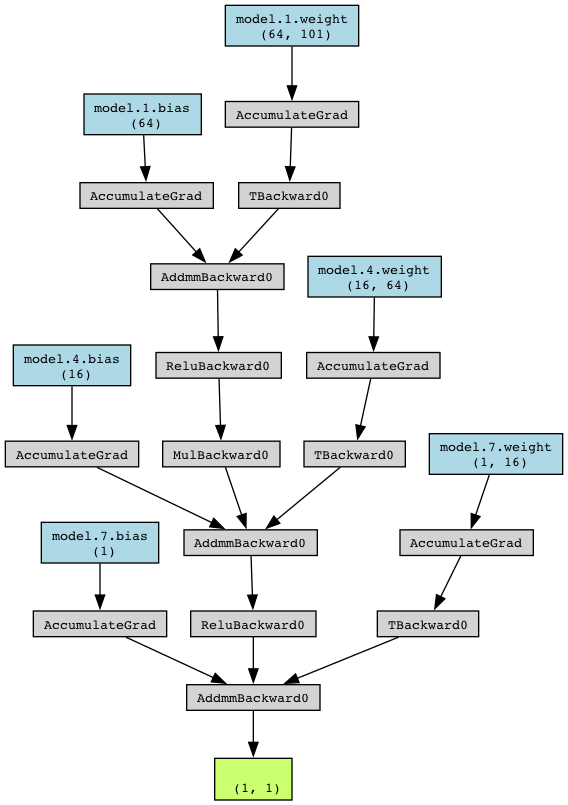
\includegraphics[width=3.5in]{viz.png}
  \caption{The neural network.}
  \label{fig:thennet}
  \end{figure}

  The network was implemented in python using the \texttt{torch} library and
  \texttt{pytorch\_lightning} tools. This network is not trained as a classifier
  because we want it to be able to generalize first and second order systems to
  fractional orders between them, so the loss function is the mean squared error
  function, \texttt{mse\_loss()}, and the optimization method adopted was Adam
  optimizer, \texttt{torch.optim.Adam()} with a learning rate of $0.001$. A
  branch of our github repository that should repeatably replicate the results
  presented in this paper is at \cite{Goodwine_Integer_trained_neural}.

\subsection{Integer Order Training, Validation and Testing Data}

  An individual element of the training, validation and training sets is the
  step response for a first or second order system (not fractional order). The
  manner in which they are generated is:

  \begin{itemize}

    \item Select a value from a uniform random distribution between 0 and 1, and
    if the value is less than 0.5, then the step response will be for a second
    order system, and if not, then it will be for a first order system.

    \item Select two numbers, $c_1$ and $c_2$ from a uniform distribution with
    values between 0.01 and 4.

    \begin{itemize}

      \item If the response is for a first order system, then the transfer
      function is
      \[
        G(s) = \frac{c_2}{c_1 s + c_2}.
      \]

      \item If the response is for a second order system, then the selected
      transfer function is
      \[
        G(s) = \frac{c_2}{c_1 s^2 + c_2}.
      \]

    \end{itemize}

	\item The unit step response from 0 to 10 seconds for the transfer function
	  is generated using the \texttt{control.step\_response()} function from the
	  python control system library. The number of time steps in the response is
	  determined by the step response function. It is then sampled every 0.1
	  second so that the length of the response vector is 101.

\end{itemize} 

    Using this method we generate a set of 100,000 first or second order step
    responses with approximately the same number of first and second order
    responses. The training set is split into three subsets: 60,000 training
    elements, 20,000 validation elements and 20,000 testing elements. For
    training, the training set is shuffled at the beginning of each epoch and
    the optimization method is applied to change the weights in the network.  At
    the end of the epoch, the network is run on the validation set to compute an
    error for data points the network was not trained on. Evidence of
    overtraining would be if the validation set error decreases and then
    increases.  At the end of all the training, the error for the testing set is
    computed.

 
Figure~\ref{fig:epochs} illustrates the error on the validation set for 10
training runs for the network versus epoch. It appears that if the validation
error increases, it tends to start to do so around 1000 epochs; otherwise it
tends to stop changing around 1000 epochs (there seems to be one exception). As
such, we will fix the number of training epochs at 1000.  Additionally, various
alternative configurations to the network described above, including more hidden
nodes and different activation functions were investigated, and the
configuration presented above generally gave the best results. 

\begin{figure}
\centering
%% Creator: Matplotlib, PGF backend
%%
%% To include the figure in your LaTeX document, write
%%   \input{<filename>.pgf}
%%
%% Make sure the required packages are loaded in your preamble
%%   \usepackage{pgf}
%%
%% Also ensure that all the required font packages are loaded; for instance,
%% the lmodern package is sometimes necessary when using math font.
%%   \usepackage{lmodern}
%%
%% Figures using additional raster images can only be included by \input if
%% they are in the same directory as the main LaTeX file. For loading figures
%% from other directories you can use the `import` package
%%   \usepackage{import}
%%
%% and then include the figures with
%%   \import{<path to file>}{<filename>.pgf}
%%
%% Matplotlib used the following preamble
%%   \def\mathdefault#1{#1}
%%   \everymath=\expandafter{\the\everymath\displaystyle}
%%   
%%   \usepackage{fontspec}
%%   \setmainfont{DejaVuSerif.ttf}[Path=\detokenize{/Users/billgoodwine/research/step/steps/lib/python3.11/site-packages/matplotlib/mpl-data/fonts/ttf/}]
%%   \setsansfont{DejaVuSans.ttf}[Path=\detokenize{/Users/billgoodwine/research/step/steps/lib/python3.11/site-packages/matplotlib/mpl-data/fonts/ttf/}]
%%   \setmonofont{DejaVuSansMono.ttf}[Path=\detokenize{/Users/billgoodwine/research/step/steps/lib/python3.11/site-packages/matplotlib/mpl-data/fonts/ttf/}]
%%   \makeatletter\@ifpackageloaded{underscore}{}{\usepackage[strings]{underscore}}\makeatother
%%
\begingroup%
\makeatletter%
\begin{pgfpicture}%
\pgfpathrectangle{\pgfpointorigin}{\pgfqpoint{3.150000in}{2.141488in}}%
\pgfusepath{use as bounding box, clip}%
\begin{pgfscope}%
\pgfsetbuttcap%
\pgfsetmiterjoin%
\definecolor{currentfill}{rgb}{1.000000,1.000000,1.000000}%
\pgfsetfillcolor{currentfill}%
\pgfsetlinewidth{0.000000pt}%
\definecolor{currentstroke}{rgb}{1.000000,1.000000,1.000000}%
\pgfsetstrokecolor{currentstroke}%
\pgfsetdash{}{0pt}%
\pgfpathmoveto{\pgfqpoint{0.000000in}{0.000000in}}%
\pgfpathlineto{\pgfqpoint{3.150000in}{0.000000in}}%
\pgfpathlineto{\pgfqpoint{3.150000in}{2.141488in}}%
\pgfpathlineto{\pgfqpoint{0.000000in}{2.141488in}}%
\pgfpathlineto{\pgfqpoint{0.000000in}{0.000000in}}%
\pgfpathclose%
\pgfusepath{fill}%
\end{pgfscope}%
\begin{pgfscope}%
\pgfsetbuttcap%
\pgfsetmiterjoin%
\definecolor{currentfill}{rgb}{1.000000,1.000000,1.000000}%
\pgfsetfillcolor{currentfill}%
\pgfsetlinewidth{0.000000pt}%
\definecolor{currentstroke}{rgb}{0.000000,0.000000,0.000000}%
\pgfsetstrokecolor{currentstroke}%
\pgfsetstrokeopacity{0.000000}%
\pgfsetdash{}{0pt}%
\pgfpathmoveto{\pgfqpoint{0.616863in}{0.463273in}}%
\pgfpathlineto{\pgfqpoint{3.080247in}{0.463273in}}%
\pgfpathlineto{\pgfqpoint{3.080247in}{2.099818in}}%
\pgfpathlineto{\pgfqpoint{0.616863in}{2.099818in}}%
\pgfpathlineto{\pgfqpoint{0.616863in}{0.463273in}}%
\pgfpathclose%
\pgfusepath{fill}%
\end{pgfscope}%
\begin{pgfscope}%
\pgfpathrectangle{\pgfqpoint{0.616863in}{0.463273in}}{\pgfqpoint{2.463384in}{1.636544in}}%
\pgfusepath{clip}%
\pgfsetrectcap%
\pgfsetroundjoin%
\pgfsetlinewidth{0.803000pt}%
\definecolor{currentstroke}{rgb}{0.690196,0.690196,0.690196}%
\pgfsetstrokecolor{currentstroke}%
\pgfsetdash{}{0pt}%
\pgfpathmoveto{\pgfqpoint{0.723220in}{0.463273in}}%
\pgfpathlineto{\pgfqpoint{0.723220in}{2.099818in}}%
\pgfusepath{stroke}%
\end{pgfscope}%
\begin{pgfscope}%
\pgfsetbuttcap%
\pgfsetroundjoin%
\definecolor{currentfill}{rgb}{0.000000,0.000000,0.000000}%
\pgfsetfillcolor{currentfill}%
\pgfsetlinewidth{0.803000pt}%
\definecolor{currentstroke}{rgb}{0.000000,0.000000,0.000000}%
\pgfsetstrokecolor{currentstroke}%
\pgfsetdash{}{0pt}%
\pgfsys@defobject{currentmarker}{\pgfqpoint{0.000000in}{-0.048611in}}{\pgfqpoint{0.000000in}{0.000000in}}{%
\pgfpathmoveto{\pgfqpoint{0.000000in}{0.000000in}}%
\pgfpathlineto{\pgfqpoint{0.000000in}{-0.048611in}}%
\pgfusepath{stroke,fill}%
}%
\begin{pgfscope}%
\pgfsys@transformshift{0.723220in}{0.463273in}%
\pgfsys@useobject{currentmarker}{}%
\end{pgfscope}%
\end{pgfscope}%
\begin{pgfscope}%
\definecolor{textcolor}{rgb}{0.000000,0.000000,0.000000}%
\pgfsetstrokecolor{textcolor}%
\pgfsetfillcolor{textcolor}%
\pgftext[x=0.723220in,y=0.366051in,,top]{\color{textcolor}{\rmfamily\fontsize{10.000000}{12.000000}\selectfont\catcode`\^=\active\def^{\ifmmode\sp\else\^{}\fi}\catcode`\%=\active\def%{\%}$\mathdefault{0}$}}%
\end{pgfscope}%
\begin{pgfscope}%
\pgfpathrectangle{\pgfqpoint{0.616863in}{0.463273in}}{\pgfqpoint{2.463384in}{1.636544in}}%
\pgfusepath{clip}%
\pgfsetrectcap%
\pgfsetroundjoin%
\pgfsetlinewidth{0.803000pt}%
\definecolor{currentstroke}{rgb}{0.690196,0.690196,0.690196}%
\pgfsetstrokecolor{currentstroke}%
\pgfsetdash{}{0pt}%
\pgfpathmoveto{\pgfqpoint{1.284764in}{0.463273in}}%
\pgfpathlineto{\pgfqpoint{1.284764in}{2.099818in}}%
\pgfusepath{stroke}%
\end{pgfscope}%
\begin{pgfscope}%
\pgfsetbuttcap%
\pgfsetroundjoin%
\definecolor{currentfill}{rgb}{0.000000,0.000000,0.000000}%
\pgfsetfillcolor{currentfill}%
\pgfsetlinewidth{0.803000pt}%
\definecolor{currentstroke}{rgb}{0.000000,0.000000,0.000000}%
\pgfsetstrokecolor{currentstroke}%
\pgfsetdash{}{0pt}%
\pgfsys@defobject{currentmarker}{\pgfqpoint{0.000000in}{-0.048611in}}{\pgfqpoint{0.000000in}{0.000000in}}{%
\pgfpathmoveto{\pgfqpoint{0.000000in}{0.000000in}}%
\pgfpathlineto{\pgfqpoint{0.000000in}{-0.048611in}}%
\pgfusepath{stroke,fill}%
}%
\begin{pgfscope}%
\pgfsys@transformshift{1.284764in}{0.463273in}%
\pgfsys@useobject{currentmarker}{}%
\end{pgfscope}%
\end{pgfscope}%
\begin{pgfscope}%
\definecolor{textcolor}{rgb}{0.000000,0.000000,0.000000}%
\pgfsetstrokecolor{textcolor}%
\pgfsetfillcolor{textcolor}%
\pgftext[x=1.284764in,y=0.366051in,,top]{\color{textcolor}{\rmfamily\fontsize{10.000000}{12.000000}\selectfont\catcode`\^=\active\def^{\ifmmode\sp\else\^{}\fi}\catcode`\%=\active\def%{\%}$\mathdefault{500}$}}%
\end{pgfscope}%
\begin{pgfscope}%
\pgfpathrectangle{\pgfqpoint{0.616863in}{0.463273in}}{\pgfqpoint{2.463384in}{1.636544in}}%
\pgfusepath{clip}%
\pgfsetrectcap%
\pgfsetroundjoin%
\pgfsetlinewidth{0.803000pt}%
\definecolor{currentstroke}{rgb}{0.690196,0.690196,0.690196}%
\pgfsetstrokecolor{currentstroke}%
\pgfsetdash{}{0pt}%
\pgfpathmoveto{\pgfqpoint{1.846309in}{0.463273in}}%
\pgfpathlineto{\pgfqpoint{1.846309in}{2.099818in}}%
\pgfusepath{stroke}%
\end{pgfscope}%
\begin{pgfscope}%
\pgfsetbuttcap%
\pgfsetroundjoin%
\definecolor{currentfill}{rgb}{0.000000,0.000000,0.000000}%
\pgfsetfillcolor{currentfill}%
\pgfsetlinewidth{0.803000pt}%
\definecolor{currentstroke}{rgb}{0.000000,0.000000,0.000000}%
\pgfsetstrokecolor{currentstroke}%
\pgfsetdash{}{0pt}%
\pgfsys@defobject{currentmarker}{\pgfqpoint{0.000000in}{-0.048611in}}{\pgfqpoint{0.000000in}{0.000000in}}{%
\pgfpathmoveto{\pgfqpoint{0.000000in}{0.000000in}}%
\pgfpathlineto{\pgfqpoint{0.000000in}{-0.048611in}}%
\pgfusepath{stroke,fill}%
}%
\begin{pgfscope}%
\pgfsys@transformshift{1.846309in}{0.463273in}%
\pgfsys@useobject{currentmarker}{}%
\end{pgfscope}%
\end{pgfscope}%
\begin{pgfscope}%
\definecolor{textcolor}{rgb}{0.000000,0.000000,0.000000}%
\pgfsetstrokecolor{textcolor}%
\pgfsetfillcolor{textcolor}%
\pgftext[x=1.846309in,y=0.366051in,,top]{\color{textcolor}{\rmfamily\fontsize{10.000000}{12.000000}\selectfont\catcode`\^=\active\def^{\ifmmode\sp\else\^{}\fi}\catcode`\%=\active\def%{\%}$\mathdefault{1000}$}}%
\end{pgfscope}%
\begin{pgfscope}%
\pgfpathrectangle{\pgfqpoint{0.616863in}{0.463273in}}{\pgfqpoint{2.463384in}{1.636544in}}%
\pgfusepath{clip}%
\pgfsetrectcap%
\pgfsetroundjoin%
\pgfsetlinewidth{0.803000pt}%
\definecolor{currentstroke}{rgb}{0.690196,0.690196,0.690196}%
\pgfsetstrokecolor{currentstroke}%
\pgfsetdash{}{0pt}%
\pgfpathmoveto{\pgfqpoint{2.407853in}{0.463273in}}%
\pgfpathlineto{\pgfqpoint{2.407853in}{2.099818in}}%
\pgfusepath{stroke}%
\end{pgfscope}%
\begin{pgfscope}%
\pgfsetbuttcap%
\pgfsetroundjoin%
\definecolor{currentfill}{rgb}{0.000000,0.000000,0.000000}%
\pgfsetfillcolor{currentfill}%
\pgfsetlinewidth{0.803000pt}%
\definecolor{currentstroke}{rgb}{0.000000,0.000000,0.000000}%
\pgfsetstrokecolor{currentstroke}%
\pgfsetdash{}{0pt}%
\pgfsys@defobject{currentmarker}{\pgfqpoint{0.000000in}{-0.048611in}}{\pgfqpoint{0.000000in}{0.000000in}}{%
\pgfpathmoveto{\pgfqpoint{0.000000in}{0.000000in}}%
\pgfpathlineto{\pgfqpoint{0.000000in}{-0.048611in}}%
\pgfusepath{stroke,fill}%
}%
\begin{pgfscope}%
\pgfsys@transformshift{2.407853in}{0.463273in}%
\pgfsys@useobject{currentmarker}{}%
\end{pgfscope}%
\end{pgfscope}%
\begin{pgfscope}%
\definecolor{textcolor}{rgb}{0.000000,0.000000,0.000000}%
\pgfsetstrokecolor{textcolor}%
\pgfsetfillcolor{textcolor}%
\pgftext[x=2.407853in,y=0.366051in,,top]{\color{textcolor}{\rmfamily\fontsize{10.000000}{12.000000}\selectfont\catcode`\^=\active\def^{\ifmmode\sp\else\^{}\fi}\catcode`\%=\active\def%{\%}$\mathdefault{1500}$}}%
\end{pgfscope}%
\begin{pgfscope}%
\pgfpathrectangle{\pgfqpoint{0.616863in}{0.463273in}}{\pgfqpoint{2.463384in}{1.636544in}}%
\pgfusepath{clip}%
\pgfsetrectcap%
\pgfsetroundjoin%
\pgfsetlinewidth{0.803000pt}%
\definecolor{currentstroke}{rgb}{0.690196,0.690196,0.690196}%
\pgfsetstrokecolor{currentstroke}%
\pgfsetdash{}{0pt}%
\pgfpathmoveto{\pgfqpoint{2.969398in}{0.463273in}}%
\pgfpathlineto{\pgfqpoint{2.969398in}{2.099818in}}%
\pgfusepath{stroke}%
\end{pgfscope}%
\begin{pgfscope}%
\pgfsetbuttcap%
\pgfsetroundjoin%
\definecolor{currentfill}{rgb}{0.000000,0.000000,0.000000}%
\pgfsetfillcolor{currentfill}%
\pgfsetlinewidth{0.803000pt}%
\definecolor{currentstroke}{rgb}{0.000000,0.000000,0.000000}%
\pgfsetstrokecolor{currentstroke}%
\pgfsetdash{}{0pt}%
\pgfsys@defobject{currentmarker}{\pgfqpoint{0.000000in}{-0.048611in}}{\pgfqpoint{0.000000in}{0.000000in}}{%
\pgfpathmoveto{\pgfqpoint{0.000000in}{0.000000in}}%
\pgfpathlineto{\pgfqpoint{0.000000in}{-0.048611in}}%
\pgfusepath{stroke,fill}%
}%
\begin{pgfscope}%
\pgfsys@transformshift{2.969398in}{0.463273in}%
\pgfsys@useobject{currentmarker}{}%
\end{pgfscope}%
\end{pgfscope}%
\begin{pgfscope}%
\definecolor{textcolor}{rgb}{0.000000,0.000000,0.000000}%
\pgfsetstrokecolor{textcolor}%
\pgfsetfillcolor{textcolor}%
\pgftext[x=2.969398in,y=0.366051in,,top]{\color{textcolor}{\rmfamily\fontsize{10.000000}{12.000000}\selectfont\catcode`\^=\active\def^{\ifmmode\sp\else\^{}\fi}\catcode`\%=\active\def%{\%}$\mathdefault{2000}$}}%
\end{pgfscope}%
\begin{pgfscope}%
\definecolor{textcolor}{rgb}{0.000000,0.000000,0.000000}%
\pgfsetstrokecolor{textcolor}%
\pgfsetfillcolor{textcolor}%
\pgftext[x=1.848555in,y=0.176083in,,top]{\color{textcolor}{\rmfamily\fontsize{10.000000}{12.000000}\selectfont\catcode`\^=\active\def^{\ifmmode\sp\else\^{}\fi}\catcode`\%=\active\def%{\%}epoch}}%
\end{pgfscope}%
\begin{pgfscope}%
\pgfpathrectangle{\pgfqpoint{0.616863in}{0.463273in}}{\pgfqpoint{2.463384in}{1.636544in}}%
\pgfusepath{clip}%
\pgfsetrectcap%
\pgfsetroundjoin%
\pgfsetlinewidth{0.803000pt}%
\definecolor{currentstroke}{rgb}{0.690196,0.690196,0.690196}%
\pgfsetstrokecolor{currentstroke}%
\pgfsetdash{}{0pt}%
\pgfpathmoveto{\pgfqpoint{0.616863in}{0.889271in}}%
\pgfpathlineto{\pgfqpoint{3.080247in}{0.889271in}}%
\pgfusepath{stroke}%
\end{pgfscope}%
\begin{pgfscope}%
\pgfsetbuttcap%
\pgfsetroundjoin%
\definecolor{currentfill}{rgb}{0.000000,0.000000,0.000000}%
\pgfsetfillcolor{currentfill}%
\pgfsetlinewidth{0.803000pt}%
\definecolor{currentstroke}{rgb}{0.000000,0.000000,0.000000}%
\pgfsetstrokecolor{currentstroke}%
\pgfsetdash{}{0pt}%
\pgfsys@defobject{currentmarker}{\pgfqpoint{-0.048611in}{0.000000in}}{\pgfqpoint{-0.000000in}{0.000000in}}{%
\pgfpathmoveto{\pgfqpoint{-0.000000in}{0.000000in}}%
\pgfpathlineto{\pgfqpoint{-0.048611in}{0.000000in}}%
\pgfusepath{stroke,fill}%
}%
\begin{pgfscope}%
\pgfsys@transformshift{0.616863in}{0.889271in}%
\pgfsys@useobject{currentmarker}{}%
\end{pgfscope}%
\end{pgfscope}%
\begin{pgfscope}%
\definecolor{textcolor}{rgb}{0.000000,0.000000,0.000000}%
\pgfsetstrokecolor{textcolor}%
\pgfsetfillcolor{textcolor}%
\pgftext[x=0.231638in, y=0.836509in, left, base]{\color{textcolor}{\rmfamily\fontsize{10.000000}{12.000000}\selectfont\catcode`\^=\active\def^{\ifmmode\sp\else\^{}\fi}\catcode`\%=\active\def%{\%}$\mathdefault{10^{-2}}$}}%
\end{pgfscope}%
\begin{pgfscope}%
\pgfpathrectangle{\pgfqpoint{0.616863in}{0.463273in}}{\pgfqpoint{2.463384in}{1.636544in}}%
\pgfusepath{clip}%
\pgfsetrectcap%
\pgfsetroundjoin%
\pgfsetlinewidth{0.803000pt}%
\definecolor{currentstroke}{rgb}{0.690196,0.690196,0.690196}%
\pgfsetstrokecolor{currentstroke}%
\pgfsetdash{}{0pt}%
\pgfpathmoveto{\pgfqpoint{0.616863in}{1.346418in}}%
\pgfpathlineto{\pgfqpoint{3.080247in}{1.346418in}}%
\pgfusepath{stroke}%
\end{pgfscope}%
\begin{pgfscope}%
\pgfsetbuttcap%
\pgfsetroundjoin%
\definecolor{currentfill}{rgb}{0.000000,0.000000,0.000000}%
\pgfsetfillcolor{currentfill}%
\pgfsetlinewidth{0.803000pt}%
\definecolor{currentstroke}{rgb}{0.000000,0.000000,0.000000}%
\pgfsetstrokecolor{currentstroke}%
\pgfsetdash{}{0pt}%
\pgfsys@defobject{currentmarker}{\pgfqpoint{-0.048611in}{0.000000in}}{\pgfqpoint{-0.000000in}{0.000000in}}{%
\pgfpathmoveto{\pgfqpoint{-0.000000in}{0.000000in}}%
\pgfpathlineto{\pgfqpoint{-0.048611in}{0.000000in}}%
\pgfusepath{stroke,fill}%
}%
\begin{pgfscope}%
\pgfsys@transformshift{0.616863in}{1.346418in}%
\pgfsys@useobject{currentmarker}{}%
\end{pgfscope}%
\end{pgfscope}%
\begin{pgfscope}%
\definecolor{textcolor}{rgb}{0.000000,0.000000,0.000000}%
\pgfsetstrokecolor{textcolor}%
\pgfsetfillcolor{textcolor}%
\pgftext[x=0.231638in, y=1.293656in, left, base]{\color{textcolor}{\rmfamily\fontsize{10.000000}{12.000000}\selectfont\catcode`\^=\active\def^{\ifmmode\sp\else\^{}\fi}\catcode`\%=\active\def%{\%}$\mathdefault{10^{-1}}$}}%
\end{pgfscope}%
\begin{pgfscope}%
\pgfpathrectangle{\pgfqpoint{0.616863in}{0.463273in}}{\pgfqpoint{2.463384in}{1.636544in}}%
\pgfusepath{clip}%
\pgfsetrectcap%
\pgfsetroundjoin%
\pgfsetlinewidth{0.803000pt}%
\definecolor{currentstroke}{rgb}{0.690196,0.690196,0.690196}%
\pgfsetstrokecolor{currentstroke}%
\pgfsetdash{}{0pt}%
\pgfpathmoveto{\pgfqpoint{0.616863in}{1.803564in}}%
\pgfpathlineto{\pgfqpoint{3.080247in}{1.803564in}}%
\pgfusepath{stroke}%
\end{pgfscope}%
\begin{pgfscope}%
\pgfsetbuttcap%
\pgfsetroundjoin%
\definecolor{currentfill}{rgb}{0.000000,0.000000,0.000000}%
\pgfsetfillcolor{currentfill}%
\pgfsetlinewidth{0.803000pt}%
\definecolor{currentstroke}{rgb}{0.000000,0.000000,0.000000}%
\pgfsetstrokecolor{currentstroke}%
\pgfsetdash{}{0pt}%
\pgfsys@defobject{currentmarker}{\pgfqpoint{-0.048611in}{0.000000in}}{\pgfqpoint{-0.000000in}{0.000000in}}{%
\pgfpathmoveto{\pgfqpoint{-0.000000in}{0.000000in}}%
\pgfpathlineto{\pgfqpoint{-0.048611in}{0.000000in}}%
\pgfusepath{stroke,fill}%
}%
\begin{pgfscope}%
\pgfsys@transformshift{0.616863in}{1.803564in}%
\pgfsys@useobject{currentmarker}{}%
\end{pgfscope}%
\end{pgfscope}%
\begin{pgfscope}%
\definecolor{textcolor}{rgb}{0.000000,0.000000,0.000000}%
\pgfsetstrokecolor{textcolor}%
\pgfsetfillcolor{textcolor}%
\pgftext[x=0.318444in, y=1.750803in, left, base]{\color{textcolor}{\rmfamily\fontsize{10.000000}{12.000000}\selectfont\catcode`\^=\active\def^{\ifmmode\sp\else\^{}\fi}\catcode`\%=\active\def%{\%}$\mathdefault{10^{0}}$}}%
\end{pgfscope}%
\begin{pgfscope}%
\pgfsetbuttcap%
\pgfsetroundjoin%
\definecolor{currentfill}{rgb}{0.000000,0.000000,0.000000}%
\pgfsetfillcolor{currentfill}%
\pgfsetlinewidth{0.602250pt}%
\definecolor{currentstroke}{rgb}{0.000000,0.000000,0.000000}%
\pgfsetstrokecolor{currentstroke}%
\pgfsetdash{}{0pt}%
\pgfsys@defobject{currentmarker}{\pgfqpoint{-0.027778in}{0.000000in}}{\pgfqpoint{-0.000000in}{0.000000in}}{%
\pgfpathmoveto{\pgfqpoint{-0.000000in}{0.000000in}}%
\pgfpathlineto{\pgfqpoint{-0.027778in}{0.000000in}}%
\pgfusepath{stroke,fill}%
}%
\begin{pgfscope}%
\pgfsys@transformshift{0.616863in}{0.569739in}%
\pgfsys@useobject{currentmarker}{}%
\end{pgfscope}%
\end{pgfscope}%
\begin{pgfscope}%
\pgfsetbuttcap%
\pgfsetroundjoin%
\definecolor{currentfill}{rgb}{0.000000,0.000000,0.000000}%
\pgfsetfillcolor{currentfill}%
\pgfsetlinewidth{0.602250pt}%
\definecolor{currentstroke}{rgb}{0.000000,0.000000,0.000000}%
\pgfsetstrokecolor{currentstroke}%
\pgfsetdash{}{0pt}%
\pgfsys@defobject{currentmarker}{\pgfqpoint{-0.027778in}{0.000000in}}{\pgfqpoint{-0.000000in}{0.000000in}}{%
\pgfpathmoveto{\pgfqpoint{-0.000000in}{0.000000in}}%
\pgfpathlineto{\pgfqpoint{-0.027778in}{0.000000in}}%
\pgfusepath{stroke,fill}%
}%
\begin{pgfscope}%
\pgfsys@transformshift{0.616863in}{0.650238in}%
\pgfsys@useobject{currentmarker}{}%
\end{pgfscope}%
\end{pgfscope}%
\begin{pgfscope}%
\pgfsetbuttcap%
\pgfsetroundjoin%
\definecolor{currentfill}{rgb}{0.000000,0.000000,0.000000}%
\pgfsetfillcolor{currentfill}%
\pgfsetlinewidth{0.602250pt}%
\definecolor{currentstroke}{rgb}{0.000000,0.000000,0.000000}%
\pgfsetstrokecolor{currentstroke}%
\pgfsetdash{}{0pt}%
\pgfsys@defobject{currentmarker}{\pgfqpoint{-0.027778in}{0.000000in}}{\pgfqpoint{-0.000000in}{0.000000in}}{%
\pgfpathmoveto{\pgfqpoint{-0.000000in}{0.000000in}}%
\pgfpathlineto{\pgfqpoint{-0.027778in}{0.000000in}}%
\pgfusepath{stroke,fill}%
}%
\begin{pgfscope}%
\pgfsys@transformshift{0.616863in}{0.707354in}%
\pgfsys@useobject{currentmarker}{}%
\end{pgfscope}%
\end{pgfscope}%
\begin{pgfscope}%
\pgfsetbuttcap%
\pgfsetroundjoin%
\definecolor{currentfill}{rgb}{0.000000,0.000000,0.000000}%
\pgfsetfillcolor{currentfill}%
\pgfsetlinewidth{0.602250pt}%
\definecolor{currentstroke}{rgb}{0.000000,0.000000,0.000000}%
\pgfsetstrokecolor{currentstroke}%
\pgfsetdash{}{0pt}%
\pgfsys@defobject{currentmarker}{\pgfqpoint{-0.027778in}{0.000000in}}{\pgfqpoint{-0.000000in}{0.000000in}}{%
\pgfpathmoveto{\pgfqpoint{-0.000000in}{0.000000in}}%
\pgfpathlineto{\pgfqpoint{-0.027778in}{0.000000in}}%
\pgfusepath{stroke,fill}%
}%
\begin{pgfscope}%
\pgfsys@transformshift{0.616863in}{0.751656in}%
\pgfsys@useobject{currentmarker}{}%
\end{pgfscope}%
\end{pgfscope}%
\begin{pgfscope}%
\pgfsetbuttcap%
\pgfsetroundjoin%
\definecolor{currentfill}{rgb}{0.000000,0.000000,0.000000}%
\pgfsetfillcolor{currentfill}%
\pgfsetlinewidth{0.602250pt}%
\definecolor{currentstroke}{rgb}{0.000000,0.000000,0.000000}%
\pgfsetstrokecolor{currentstroke}%
\pgfsetdash{}{0pt}%
\pgfsys@defobject{currentmarker}{\pgfqpoint{-0.027778in}{0.000000in}}{\pgfqpoint{-0.000000in}{0.000000in}}{%
\pgfpathmoveto{\pgfqpoint{-0.000000in}{0.000000in}}%
\pgfpathlineto{\pgfqpoint{-0.027778in}{0.000000in}}%
\pgfusepath{stroke,fill}%
}%
\begin{pgfscope}%
\pgfsys@transformshift{0.616863in}{0.787853in}%
\pgfsys@useobject{currentmarker}{}%
\end{pgfscope}%
\end{pgfscope}%
\begin{pgfscope}%
\pgfsetbuttcap%
\pgfsetroundjoin%
\definecolor{currentfill}{rgb}{0.000000,0.000000,0.000000}%
\pgfsetfillcolor{currentfill}%
\pgfsetlinewidth{0.602250pt}%
\definecolor{currentstroke}{rgb}{0.000000,0.000000,0.000000}%
\pgfsetstrokecolor{currentstroke}%
\pgfsetdash{}{0pt}%
\pgfsys@defobject{currentmarker}{\pgfqpoint{-0.027778in}{0.000000in}}{\pgfqpoint{-0.000000in}{0.000000in}}{%
\pgfpathmoveto{\pgfqpoint{-0.000000in}{0.000000in}}%
\pgfpathlineto{\pgfqpoint{-0.027778in}{0.000000in}}%
\pgfusepath{stroke,fill}%
}%
\begin{pgfscope}%
\pgfsys@transformshift{0.616863in}{0.818458in}%
\pgfsys@useobject{currentmarker}{}%
\end{pgfscope}%
\end{pgfscope}%
\begin{pgfscope}%
\pgfsetbuttcap%
\pgfsetroundjoin%
\definecolor{currentfill}{rgb}{0.000000,0.000000,0.000000}%
\pgfsetfillcolor{currentfill}%
\pgfsetlinewidth{0.602250pt}%
\definecolor{currentstroke}{rgb}{0.000000,0.000000,0.000000}%
\pgfsetstrokecolor{currentstroke}%
\pgfsetdash{}{0pt}%
\pgfsys@defobject{currentmarker}{\pgfqpoint{-0.027778in}{0.000000in}}{\pgfqpoint{-0.000000in}{0.000000in}}{%
\pgfpathmoveto{\pgfqpoint{-0.000000in}{0.000000in}}%
\pgfpathlineto{\pgfqpoint{-0.027778in}{0.000000in}}%
\pgfusepath{stroke,fill}%
}%
\begin{pgfscope}%
\pgfsys@transformshift{0.616863in}{0.844969in}%
\pgfsys@useobject{currentmarker}{}%
\end{pgfscope}%
\end{pgfscope}%
\begin{pgfscope}%
\pgfsetbuttcap%
\pgfsetroundjoin%
\definecolor{currentfill}{rgb}{0.000000,0.000000,0.000000}%
\pgfsetfillcolor{currentfill}%
\pgfsetlinewidth{0.602250pt}%
\definecolor{currentstroke}{rgb}{0.000000,0.000000,0.000000}%
\pgfsetstrokecolor{currentstroke}%
\pgfsetdash{}{0pt}%
\pgfsys@defobject{currentmarker}{\pgfqpoint{-0.027778in}{0.000000in}}{\pgfqpoint{-0.000000in}{0.000000in}}{%
\pgfpathmoveto{\pgfqpoint{-0.000000in}{0.000000in}}%
\pgfpathlineto{\pgfqpoint{-0.027778in}{0.000000in}}%
\pgfusepath{stroke,fill}%
}%
\begin{pgfscope}%
\pgfsys@transformshift{0.616863in}{0.868353in}%
\pgfsys@useobject{currentmarker}{}%
\end{pgfscope}%
\end{pgfscope}%
\begin{pgfscope}%
\pgfsetbuttcap%
\pgfsetroundjoin%
\definecolor{currentfill}{rgb}{0.000000,0.000000,0.000000}%
\pgfsetfillcolor{currentfill}%
\pgfsetlinewidth{0.602250pt}%
\definecolor{currentstroke}{rgb}{0.000000,0.000000,0.000000}%
\pgfsetstrokecolor{currentstroke}%
\pgfsetdash{}{0pt}%
\pgfsys@defobject{currentmarker}{\pgfqpoint{-0.027778in}{0.000000in}}{\pgfqpoint{-0.000000in}{0.000000in}}{%
\pgfpathmoveto{\pgfqpoint{-0.000000in}{0.000000in}}%
\pgfpathlineto{\pgfqpoint{-0.027778in}{0.000000in}}%
\pgfusepath{stroke,fill}%
}%
\begin{pgfscope}%
\pgfsys@transformshift{0.616863in}{1.026886in}%
\pgfsys@useobject{currentmarker}{}%
\end{pgfscope}%
\end{pgfscope}%
\begin{pgfscope}%
\pgfsetbuttcap%
\pgfsetroundjoin%
\definecolor{currentfill}{rgb}{0.000000,0.000000,0.000000}%
\pgfsetfillcolor{currentfill}%
\pgfsetlinewidth{0.602250pt}%
\definecolor{currentstroke}{rgb}{0.000000,0.000000,0.000000}%
\pgfsetstrokecolor{currentstroke}%
\pgfsetdash{}{0pt}%
\pgfsys@defobject{currentmarker}{\pgfqpoint{-0.027778in}{0.000000in}}{\pgfqpoint{-0.000000in}{0.000000in}}{%
\pgfpathmoveto{\pgfqpoint{-0.000000in}{0.000000in}}%
\pgfpathlineto{\pgfqpoint{-0.027778in}{0.000000in}}%
\pgfusepath{stroke,fill}%
}%
\begin{pgfscope}%
\pgfsys@transformshift{0.616863in}{1.107385in}%
\pgfsys@useobject{currentmarker}{}%
\end{pgfscope}%
\end{pgfscope}%
\begin{pgfscope}%
\pgfsetbuttcap%
\pgfsetroundjoin%
\definecolor{currentfill}{rgb}{0.000000,0.000000,0.000000}%
\pgfsetfillcolor{currentfill}%
\pgfsetlinewidth{0.602250pt}%
\definecolor{currentstroke}{rgb}{0.000000,0.000000,0.000000}%
\pgfsetstrokecolor{currentstroke}%
\pgfsetdash{}{0pt}%
\pgfsys@defobject{currentmarker}{\pgfqpoint{-0.027778in}{0.000000in}}{\pgfqpoint{-0.000000in}{0.000000in}}{%
\pgfpathmoveto{\pgfqpoint{-0.000000in}{0.000000in}}%
\pgfpathlineto{\pgfqpoint{-0.027778in}{0.000000in}}%
\pgfusepath{stroke,fill}%
}%
\begin{pgfscope}%
\pgfsys@transformshift{0.616863in}{1.164501in}%
\pgfsys@useobject{currentmarker}{}%
\end{pgfscope}%
\end{pgfscope}%
\begin{pgfscope}%
\pgfsetbuttcap%
\pgfsetroundjoin%
\definecolor{currentfill}{rgb}{0.000000,0.000000,0.000000}%
\pgfsetfillcolor{currentfill}%
\pgfsetlinewidth{0.602250pt}%
\definecolor{currentstroke}{rgb}{0.000000,0.000000,0.000000}%
\pgfsetstrokecolor{currentstroke}%
\pgfsetdash{}{0pt}%
\pgfsys@defobject{currentmarker}{\pgfqpoint{-0.027778in}{0.000000in}}{\pgfqpoint{-0.000000in}{0.000000in}}{%
\pgfpathmoveto{\pgfqpoint{-0.000000in}{0.000000in}}%
\pgfpathlineto{\pgfqpoint{-0.027778in}{0.000000in}}%
\pgfusepath{stroke,fill}%
}%
\begin{pgfscope}%
\pgfsys@transformshift{0.616863in}{1.208803in}%
\pgfsys@useobject{currentmarker}{}%
\end{pgfscope}%
\end{pgfscope}%
\begin{pgfscope}%
\pgfsetbuttcap%
\pgfsetroundjoin%
\definecolor{currentfill}{rgb}{0.000000,0.000000,0.000000}%
\pgfsetfillcolor{currentfill}%
\pgfsetlinewidth{0.602250pt}%
\definecolor{currentstroke}{rgb}{0.000000,0.000000,0.000000}%
\pgfsetstrokecolor{currentstroke}%
\pgfsetdash{}{0pt}%
\pgfsys@defobject{currentmarker}{\pgfqpoint{-0.027778in}{0.000000in}}{\pgfqpoint{-0.000000in}{0.000000in}}{%
\pgfpathmoveto{\pgfqpoint{-0.000000in}{0.000000in}}%
\pgfpathlineto{\pgfqpoint{-0.027778in}{0.000000in}}%
\pgfusepath{stroke,fill}%
}%
\begin{pgfscope}%
\pgfsys@transformshift{0.616863in}{1.245000in}%
\pgfsys@useobject{currentmarker}{}%
\end{pgfscope}%
\end{pgfscope}%
\begin{pgfscope}%
\pgfsetbuttcap%
\pgfsetroundjoin%
\definecolor{currentfill}{rgb}{0.000000,0.000000,0.000000}%
\pgfsetfillcolor{currentfill}%
\pgfsetlinewidth{0.602250pt}%
\definecolor{currentstroke}{rgb}{0.000000,0.000000,0.000000}%
\pgfsetstrokecolor{currentstroke}%
\pgfsetdash{}{0pt}%
\pgfsys@defobject{currentmarker}{\pgfqpoint{-0.027778in}{0.000000in}}{\pgfqpoint{-0.000000in}{0.000000in}}{%
\pgfpathmoveto{\pgfqpoint{-0.000000in}{0.000000in}}%
\pgfpathlineto{\pgfqpoint{-0.027778in}{0.000000in}}%
\pgfusepath{stroke,fill}%
}%
\begin{pgfscope}%
\pgfsys@transformshift{0.616863in}{1.275605in}%
\pgfsys@useobject{currentmarker}{}%
\end{pgfscope}%
\end{pgfscope}%
\begin{pgfscope}%
\pgfsetbuttcap%
\pgfsetroundjoin%
\definecolor{currentfill}{rgb}{0.000000,0.000000,0.000000}%
\pgfsetfillcolor{currentfill}%
\pgfsetlinewidth{0.602250pt}%
\definecolor{currentstroke}{rgb}{0.000000,0.000000,0.000000}%
\pgfsetstrokecolor{currentstroke}%
\pgfsetdash{}{0pt}%
\pgfsys@defobject{currentmarker}{\pgfqpoint{-0.027778in}{0.000000in}}{\pgfqpoint{-0.000000in}{0.000000in}}{%
\pgfpathmoveto{\pgfqpoint{-0.000000in}{0.000000in}}%
\pgfpathlineto{\pgfqpoint{-0.027778in}{0.000000in}}%
\pgfusepath{stroke,fill}%
}%
\begin{pgfscope}%
\pgfsys@transformshift{0.616863in}{1.302115in}%
\pgfsys@useobject{currentmarker}{}%
\end{pgfscope}%
\end{pgfscope}%
\begin{pgfscope}%
\pgfsetbuttcap%
\pgfsetroundjoin%
\definecolor{currentfill}{rgb}{0.000000,0.000000,0.000000}%
\pgfsetfillcolor{currentfill}%
\pgfsetlinewidth{0.602250pt}%
\definecolor{currentstroke}{rgb}{0.000000,0.000000,0.000000}%
\pgfsetstrokecolor{currentstroke}%
\pgfsetdash{}{0pt}%
\pgfsys@defobject{currentmarker}{\pgfqpoint{-0.027778in}{0.000000in}}{\pgfqpoint{-0.000000in}{0.000000in}}{%
\pgfpathmoveto{\pgfqpoint{-0.000000in}{0.000000in}}%
\pgfpathlineto{\pgfqpoint{-0.027778in}{0.000000in}}%
\pgfusepath{stroke,fill}%
}%
\begin{pgfscope}%
\pgfsys@transformshift{0.616863in}{1.325500in}%
\pgfsys@useobject{currentmarker}{}%
\end{pgfscope}%
\end{pgfscope}%
\begin{pgfscope}%
\pgfsetbuttcap%
\pgfsetroundjoin%
\definecolor{currentfill}{rgb}{0.000000,0.000000,0.000000}%
\pgfsetfillcolor{currentfill}%
\pgfsetlinewidth{0.602250pt}%
\definecolor{currentstroke}{rgb}{0.000000,0.000000,0.000000}%
\pgfsetstrokecolor{currentstroke}%
\pgfsetdash{}{0pt}%
\pgfsys@defobject{currentmarker}{\pgfqpoint{-0.027778in}{0.000000in}}{\pgfqpoint{-0.000000in}{0.000000in}}{%
\pgfpathmoveto{\pgfqpoint{-0.000000in}{0.000000in}}%
\pgfpathlineto{\pgfqpoint{-0.027778in}{0.000000in}}%
\pgfusepath{stroke,fill}%
}%
\begin{pgfscope}%
\pgfsys@transformshift{0.616863in}{1.484032in}%
\pgfsys@useobject{currentmarker}{}%
\end{pgfscope}%
\end{pgfscope}%
\begin{pgfscope}%
\pgfsetbuttcap%
\pgfsetroundjoin%
\definecolor{currentfill}{rgb}{0.000000,0.000000,0.000000}%
\pgfsetfillcolor{currentfill}%
\pgfsetlinewidth{0.602250pt}%
\definecolor{currentstroke}{rgb}{0.000000,0.000000,0.000000}%
\pgfsetstrokecolor{currentstroke}%
\pgfsetdash{}{0pt}%
\pgfsys@defobject{currentmarker}{\pgfqpoint{-0.027778in}{0.000000in}}{\pgfqpoint{-0.000000in}{0.000000in}}{%
\pgfpathmoveto{\pgfqpoint{-0.000000in}{0.000000in}}%
\pgfpathlineto{\pgfqpoint{-0.027778in}{0.000000in}}%
\pgfusepath{stroke,fill}%
}%
\begin{pgfscope}%
\pgfsys@transformshift{0.616863in}{1.564532in}%
\pgfsys@useobject{currentmarker}{}%
\end{pgfscope}%
\end{pgfscope}%
\begin{pgfscope}%
\pgfsetbuttcap%
\pgfsetroundjoin%
\definecolor{currentfill}{rgb}{0.000000,0.000000,0.000000}%
\pgfsetfillcolor{currentfill}%
\pgfsetlinewidth{0.602250pt}%
\definecolor{currentstroke}{rgb}{0.000000,0.000000,0.000000}%
\pgfsetstrokecolor{currentstroke}%
\pgfsetdash{}{0pt}%
\pgfsys@defobject{currentmarker}{\pgfqpoint{-0.027778in}{0.000000in}}{\pgfqpoint{-0.000000in}{0.000000in}}{%
\pgfpathmoveto{\pgfqpoint{-0.000000in}{0.000000in}}%
\pgfpathlineto{\pgfqpoint{-0.027778in}{0.000000in}}%
\pgfusepath{stroke,fill}%
}%
\begin{pgfscope}%
\pgfsys@transformshift{0.616863in}{1.621647in}%
\pgfsys@useobject{currentmarker}{}%
\end{pgfscope}%
\end{pgfscope}%
\begin{pgfscope}%
\pgfsetbuttcap%
\pgfsetroundjoin%
\definecolor{currentfill}{rgb}{0.000000,0.000000,0.000000}%
\pgfsetfillcolor{currentfill}%
\pgfsetlinewidth{0.602250pt}%
\definecolor{currentstroke}{rgb}{0.000000,0.000000,0.000000}%
\pgfsetstrokecolor{currentstroke}%
\pgfsetdash{}{0pt}%
\pgfsys@defobject{currentmarker}{\pgfqpoint{-0.027778in}{0.000000in}}{\pgfqpoint{-0.000000in}{0.000000in}}{%
\pgfpathmoveto{\pgfqpoint{-0.000000in}{0.000000in}}%
\pgfpathlineto{\pgfqpoint{-0.027778in}{0.000000in}}%
\pgfusepath{stroke,fill}%
}%
\begin{pgfscope}%
\pgfsys@transformshift{0.616863in}{1.665949in}%
\pgfsys@useobject{currentmarker}{}%
\end{pgfscope}%
\end{pgfscope}%
\begin{pgfscope}%
\pgfsetbuttcap%
\pgfsetroundjoin%
\definecolor{currentfill}{rgb}{0.000000,0.000000,0.000000}%
\pgfsetfillcolor{currentfill}%
\pgfsetlinewidth{0.602250pt}%
\definecolor{currentstroke}{rgb}{0.000000,0.000000,0.000000}%
\pgfsetstrokecolor{currentstroke}%
\pgfsetdash{}{0pt}%
\pgfsys@defobject{currentmarker}{\pgfqpoint{-0.027778in}{0.000000in}}{\pgfqpoint{-0.000000in}{0.000000in}}{%
\pgfpathmoveto{\pgfqpoint{-0.000000in}{0.000000in}}%
\pgfpathlineto{\pgfqpoint{-0.027778in}{0.000000in}}%
\pgfusepath{stroke,fill}%
}%
\begin{pgfscope}%
\pgfsys@transformshift{0.616863in}{1.702147in}%
\pgfsys@useobject{currentmarker}{}%
\end{pgfscope}%
\end{pgfscope}%
\begin{pgfscope}%
\pgfsetbuttcap%
\pgfsetroundjoin%
\definecolor{currentfill}{rgb}{0.000000,0.000000,0.000000}%
\pgfsetfillcolor{currentfill}%
\pgfsetlinewidth{0.602250pt}%
\definecolor{currentstroke}{rgb}{0.000000,0.000000,0.000000}%
\pgfsetstrokecolor{currentstroke}%
\pgfsetdash{}{0pt}%
\pgfsys@defobject{currentmarker}{\pgfqpoint{-0.027778in}{0.000000in}}{\pgfqpoint{-0.000000in}{0.000000in}}{%
\pgfpathmoveto{\pgfqpoint{-0.000000in}{0.000000in}}%
\pgfpathlineto{\pgfqpoint{-0.027778in}{0.000000in}}%
\pgfusepath{stroke,fill}%
}%
\begin{pgfscope}%
\pgfsys@transformshift{0.616863in}{1.732751in}%
\pgfsys@useobject{currentmarker}{}%
\end{pgfscope}%
\end{pgfscope}%
\begin{pgfscope}%
\pgfsetbuttcap%
\pgfsetroundjoin%
\definecolor{currentfill}{rgb}{0.000000,0.000000,0.000000}%
\pgfsetfillcolor{currentfill}%
\pgfsetlinewidth{0.602250pt}%
\definecolor{currentstroke}{rgb}{0.000000,0.000000,0.000000}%
\pgfsetstrokecolor{currentstroke}%
\pgfsetdash{}{0pt}%
\pgfsys@defobject{currentmarker}{\pgfqpoint{-0.027778in}{0.000000in}}{\pgfqpoint{-0.000000in}{0.000000in}}{%
\pgfpathmoveto{\pgfqpoint{-0.000000in}{0.000000in}}%
\pgfpathlineto{\pgfqpoint{-0.027778in}{0.000000in}}%
\pgfusepath{stroke,fill}%
}%
\begin{pgfscope}%
\pgfsys@transformshift{0.616863in}{1.759262in}%
\pgfsys@useobject{currentmarker}{}%
\end{pgfscope}%
\end{pgfscope}%
\begin{pgfscope}%
\pgfsetbuttcap%
\pgfsetroundjoin%
\definecolor{currentfill}{rgb}{0.000000,0.000000,0.000000}%
\pgfsetfillcolor{currentfill}%
\pgfsetlinewidth{0.602250pt}%
\definecolor{currentstroke}{rgb}{0.000000,0.000000,0.000000}%
\pgfsetstrokecolor{currentstroke}%
\pgfsetdash{}{0pt}%
\pgfsys@defobject{currentmarker}{\pgfqpoint{-0.027778in}{0.000000in}}{\pgfqpoint{-0.000000in}{0.000000in}}{%
\pgfpathmoveto{\pgfqpoint{-0.000000in}{0.000000in}}%
\pgfpathlineto{\pgfqpoint{-0.027778in}{0.000000in}}%
\pgfusepath{stroke,fill}%
}%
\begin{pgfscope}%
\pgfsys@transformshift{0.616863in}{1.782646in}%
\pgfsys@useobject{currentmarker}{}%
\end{pgfscope}%
\end{pgfscope}%
\begin{pgfscope}%
\pgfsetbuttcap%
\pgfsetroundjoin%
\definecolor{currentfill}{rgb}{0.000000,0.000000,0.000000}%
\pgfsetfillcolor{currentfill}%
\pgfsetlinewidth{0.602250pt}%
\definecolor{currentstroke}{rgb}{0.000000,0.000000,0.000000}%
\pgfsetstrokecolor{currentstroke}%
\pgfsetdash{}{0pt}%
\pgfsys@defobject{currentmarker}{\pgfqpoint{-0.027778in}{0.000000in}}{\pgfqpoint{-0.000000in}{0.000000in}}{%
\pgfpathmoveto{\pgfqpoint{-0.000000in}{0.000000in}}%
\pgfpathlineto{\pgfqpoint{-0.027778in}{0.000000in}}%
\pgfusepath{stroke,fill}%
}%
\begin{pgfscope}%
\pgfsys@transformshift{0.616863in}{1.941179in}%
\pgfsys@useobject{currentmarker}{}%
\end{pgfscope}%
\end{pgfscope}%
\begin{pgfscope}%
\pgfsetbuttcap%
\pgfsetroundjoin%
\definecolor{currentfill}{rgb}{0.000000,0.000000,0.000000}%
\pgfsetfillcolor{currentfill}%
\pgfsetlinewidth{0.602250pt}%
\definecolor{currentstroke}{rgb}{0.000000,0.000000,0.000000}%
\pgfsetstrokecolor{currentstroke}%
\pgfsetdash{}{0pt}%
\pgfsys@defobject{currentmarker}{\pgfqpoint{-0.027778in}{0.000000in}}{\pgfqpoint{-0.000000in}{0.000000in}}{%
\pgfpathmoveto{\pgfqpoint{-0.000000in}{0.000000in}}%
\pgfpathlineto{\pgfqpoint{-0.027778in}{0.000000in}}%
\pgfusepath{stroke,fill}%
}%
\begin{pgfscope}%
\pgfsys@transformshift{0.616863in}{2.021679in}%
\pgfsys@useobject{currentmarker}{}%
\end{pgfscope}%
\end{pgfscope}%
\begin{pgfscope}%
\pgfsetbuttcap%
\pgfsetroundjoin%
\definecolor{currentfill}{rgb}{0.000000,0.000000,0.000000}%
\pgfsetfillcolor{currentfill}%
\pgfsetlinewidth{0.602250pt}%
\definecolor{currentstroke}{rgb}{0.000000,0.000000,0.000000}%
\pgfsetstrokecolor{currentstroke}%
\pgfsetdash{}{0pt}%
\pgfsys@defobject{currentmarker}{\pgfqpoint{-0.027778in}{0.000000in}}{\pgfqpoint{-0.000000in}{0.000000in}}{%
\pgfpathmoveto{\pgfqpoint{-0.000000in}{0.000000in}}%
\pgfpathlineto{\pgfqpoint{-0.027778in}{0.000000in}}%
\pgfusepath{stroke,fill}%
}%
\begin{pgfscope}%
\pgfsys@transformshift{0.616863in}{2.078794in}%
\pgfsys@useobject{currentmarker}{}%
\end{pgfscope}%
\end{pgfscope}%
\begin{pgfscope}%
\definecolor{textcolor}{rgb}{0.000000,0.000000,0.000000}%
\pgfsetstrokecolor{textcolor}%
\pgfsetfillcolor{textcolor}%
\pgftext[x=0.176083in,y=1.281546in,,bottom,rotate=90.000000]{\color{textcolor}{\rmfamily\fontsize{10.000000}{12.000000}\selectfont\catcode`\^=\active\def^{\ifmmode\sp\else\^{}\fi}\catcode`\%=\active\def%{\%}Validation set error}}%
\end{pgfscope}%
\begin{pgfscope}%
\pgfpathrectangle{\pgfqpoint{0.616863in}{0.463273in}}{\pgfqpoint{2.463384in}{1.636544in}}%
\pgfusepath{clip}%
\pgfsetrectcap%
\pgfsetroundjoin%
\pgfsetlinewidth{1.505625pt}%
\definecolor{currentstroke}{rgb}{0.121569,0.466667,0.705882}%
\pgfsetstrokecolor{currentstroke}%
\pgfsetdash{}{0pt}%
\pgfpathmoveto{\pgfqpoint{0.728835in}{1.987128in}}%
\pgfpathlineto{\pgfqpoint{0.735574in}{1.945512in}}%
\pgfpathlineto{\pgfqpoint{0.742312in}{1.885687in}}%
\pgfpathlineto{\pgfqpoint{0.745681in}{1.846262in}}%
\pgfpathlineto{\pgfqpoint{0.750174in}{1.782813in}}%
\pgfpathlineto{\pgfqpoint{0.770389in}{1.442913in}}%
\pgfpathlineto{\pgfqpoint{0.773759in}{1.422333in}}%
\pgfpathlineto{\pgfqpoint{0.783866in}{1.395454in}}%
\pgfpathlineto{\pgfqpoint{0.797343in}{1.334680in}}%
\pgfpathlineto{\pgfqpoint{0.818682in}{1.275453in}}%
\pgfpathlineto{\pgfqpoint{0.842267in}{1.227116in}}%
\pgfpathlineto{\pgfqpoint{0.864729in}{1.184212in}}%
\pgfpathlineto{\pgfqpoint{0.877083in}{1.164638in}}%
\pgfpathlineto{\pgfqpoint{0.937730in}{1.074502in}}%
\pgfpathlineto{\pgfqpoint{0.969176in}{1.032321in}}%
\pgfpathlineto{\pgfqpoint{0.998376in}{0.997048in}}%
\pgfpathlineto{\pgfqpoint{1.023084in}{0.971620in}}%
\pgfpathlineto{\pgfqpoint{1.056777in}{0.939775in}}%
\pgfpathlineto{\pgfqpoint{1.103947in}{0.904064in}}%
\pgfpathlineto{\pgfqpoint{1.136516in}{0.885235in}}%
\pgfpathlineto{\pgfqpoint{1.147747in}{0.878580in}}%
\pgfpathlineto{\pgfqpoint{1.158978in}{0.873514in}}%
\pgfpathlineto{\pgfqpoint{1.206148in}{0.852027in}}%
\pgfpathlineto{\pgfqpoint{1.238717in}{0.838206in}}%
\pgfpathlineto{\pgfqpoint{1.255564in}{0.832997in}}%
\pgfpathlineto{\pgfqpoint{1.260056in}{0.830667in}}%
\pgfpathlineto{\pgfqpoint{1.300487in}{0.817901in}}%
\pgfpathlineto{\pgfqpoint{1.306103in}{0.815335in}}%
\pgfpathlineto{\pgfqpoint{1.326318in}{0.809508in}}%
\pgfpathlineto{\pgfqpoint{1.334180in}{0.806780in}}%
\pgfpathlineto{\pgfqpoint{1.342042in}{0.805234in}}%
\pgfpathlineto{\pgfqpoint{1.351026in}{0.801233in}}%
\pgfpathlineto{\pgfqpoint{1.364503in}{0.798605in}}%
\pgfpathlineto{\pgfqpoint{1.375734in}{0.795108in}}%
\pgfpathlineto{\pgfqpoint{1.397073in}{0.789748in}}%
\pgfpathlineto{\pgfqpoint{1.403812in}{0.787883in}}%
\pgfpathlineto{\pgfqpoint{1.410550in}{0.785575in}}%
\pgfpathlineto{\pgfqpoint{1.419535in}{0.783925in}}%
\pgfpathlineto{\pgfqpoint{1.425150in}{0.781913in}}%
\pgfpathlineto{\pgfqpoint{1.444243in}{0.778076in}}%
\pgfpathlineto{\pgfqpoint{1.554306in}{0.755237in}}%
\pgfpathlineto{\pgfqpoint{1.561044in}{0.753775in}}%
\pgfpathlineto{\pgfqpoint{1.567783in}{0.751757in}}%
\pgfpathlineto{\pgfqpoint{1.582383in}{0.749647in}}%
\pgfpathlineto{\pgfqpoint{1.586875in}{0.748742in}}%
\pgfpathlineto{\pgfqpoint{1.589121in}{0.748861in}}%
\pgfpathlineto{\pgfqpoint{1.593614in}{0.746769in}}%
\pgfpathlineto{\pgfqpoint{1.621691in}{0.742550in}}%
\pgfpathlineto{\pgfqpoint{1.629553in}{0.740971in}}%
\pgfpathlineto{\pgfqpoint{1.631799in}{0.741175in}}%
\pgfpathlineto{\pgfqpoint{1.641906in}{0.739041in}}%
\pgfpathlineto{\pgfqpoint{1.647522in}{0.738224in}}%
\pgfpathlineto{\pgfqpoint{1.653137in}{0.736689in}}%
\pgfpathlineto{\pgfqpoint{1.662122in}{0.736017in}}%
\pgfpathlineto{\pgfqpoint{1.664368in}{0.735033in}}%
\pgfpathlineto{\pgfqpoint{1.690199in}{0.729920in}}%
\pgfpathlineto{\pgfqpoint{1.692445in}{0.729360in}}%
\pgfpathlineto{\pgfqpoint{1.700307in}{0.729553in}}%
\pgfpathlineto{\pgfqpoint{1.713784in}{0.727006in}}%
\pgfpathlineto{\pgfqpoint{1.716030in}{0.726800in}}%
\pgfpathlineto{\pgfqpoint{1.725015in}{0.723920in}}%
\pgfpathlineto{\pgfqpoint{1.734000in}{0.722299in}}%
\pgfpathlineto{\pgfqpoint{1.753092in}{0.719283in}}%
\pgfpathlineto{\pgfqpoint{1.762077in}{0.716007in}}%
\pgfpathlineto{\pgfqpoint{1.814862in}{0.705214in}}%
\pgfpathlineto{\pgfqpoint{1.820478in}{0.704330in}}%
\pgfpathlineto{\pgfqpoint{1.826093in}{0.702391in}}%
\pgfpathlineto{\pgfqpoint{1.832832in}{0.702212in}}%
\pgfpathlineto{\pgfqpoint{1.841816in}{0.699762in}}%
\pgfpathlineto{\pgfqpoint{1.846309in}{0.700101in}}%
\pgfpathlineto{\pgfqpoint{1.856417in}{0.697419in}}%
\pgfpathlineto{\pgfqpoint{1.865401in}{0.697269in}}%
\pgfpathlineto{\pgfqpoint{1.885617in}{0.693436in}}%
\pgfpathlineto{\pgfqpoint{1.890109in}{0.691705in}}%
\pgfpathlineto{\pgfqpoint{1.894602in}{0.691185in}}%
\pgfpathlineto{\pgfqpoint{1.895725in}{0.690354in}}%
\pgfpathlineto{\pgfqpoint{1.903586in}{0.689612in}}%
\pgfpathlineto{\pgfqpoint{1.906956in}{0.686853in}}%
\pgfpathlineto{\pgfqpoint{1.910325in}{0.687171in}}%
\pgfpathlineto{\pgfqpoint{1.918186in}{0.684663in}}%
\pgfpathlineto{\pgfqpoint{1.920433in}{0.684857in}}%
\pgfpathlineto{\pgfqpoint{1.922679in}{0.683516in}}%
\pgfpathlineto{\pgfqpoint{1.939525in}{0.680256in}}%
\pgfpathlineto{\pgfqpoint{1.942894in}{0.679046in}}%
\pgfpathlineto{\pgfqpoint{1.947387in}{0.680300in}}%
\pgfpathlineto{\pgfqpoint{1.950756in}{0.676383in}}%
\pgfpathlineto{\pgfqpoint{1.957495in}{0.677795in}}%
\pgfpathlineto{\pgfqpoint{1.961987in}{0.674985in}}%
\pgfpathlineto{\pgfqpoint{1.964233in}{0.675952in}}%
\pgfpathlineto{\pgfqpoint{1.997926in}{0.670544in}}%
\pgfpathlineto{\pgfqpoint{2.001295in}{0.670534in}}%
\pgfpathlineto{\pgfqpoint{2.004664in}{0.667372in}}%
\pgfpathlineto{\pgfqpoint{2.017018in}{0.667360in}}%
\pgfpathlineto{\pgfqpoint{2.022634in}{0.665596in}}%
\pgfpathlineto{\pgfqpoint{2.026003in}{0.666790in}}%
\pgfpathlineto{\pgfqpoint{2.028249in}{0.665359in}}%
\pgfpathlineto{\pgfqpoint{2.031618in}{0.665008in}}%
\pgfpathlineto{\pgfqpoint{2.048465in}{0.662097in}}%
\pgfpathlineto{\pgfqpoint{2.051834in}{0.659188in}}%
\pgfpathlineto{\pgfqpoint{2.058573in}{0.660636in}}%
\pgfpathlineto{\pgfqpoint{2.063065in}{0.658500in}}%
\pgfpathlineto{\pgfqpoint{2.065311in}{0.658432in}}%
\pgfpathlineto{\pgfqpoint{2.068680in}{0.658141in}}%
\pgfpathlineto{\pgfqpoint{2.072050in}{0.657734in}}%
\pgfpathlineto{\pgfqpoint{2.075419in}{0.657151in}}%
\pgfpathlineto{\pgfqpoint{2.077665in}{0.657022in}}%
\pgfpathlineto{\pgfqpoint{2.079911in}{0.655442in}}%
\pgfpathlineto{\pgfqpoint{2.083281in}{0.656567in}}%
\pgfpathlineto{\pgfqpoint{2.087773in}{0.654232in}}%
\pgfpathlineto{\pgfqpoint{2.092265in}{0.654456in}}%
\pgfpathlineto{\pgfqpoint{2.111358in}{0.650275in}}%
\pgfpathlineto{\pgfqpoint{2.114727in}{0.651579in}}%
\pgfpathlineto{\pgfqpoint{2.120342in}{0.650453in}}%
\pgfpathlineto{\pgfqpoint{2.123712in}{0.650052in}}%
\pgfpathlineto{\pgfqpoint{2.127081in}{0.650136in}}%
\pgfpathlineto{\pgfqpoint{2.131573in}{0.647669in}}%
\pgfpathlineto{\pgfqpoint{2.136066in}{0.648669in}}%
\pgfpathlineto{\pgfqpoint{2.139435in}{0.645354in}}%
\pgfpathlineto{\pgfqpoint{2.143927in}{0.648338in}}%
\pgfpathlineto{\pgfqpoint{2.145050in}{0.647343in}}%
\pgfpathlineto{\pgfqpoint{2.154035in}{0.646362in}}%
\pgfpathlineto{\pgfqpoint{2.161897in}{0.644416in}}%
\pgfpathlineto{\pgfqpoint{2.170881in}{0.644270in}}%
\pgfpathlineto{\pgfqpoint{2.175374in}{0.643571in}}%
\pgfpathlineto{\pgfqpoint{2.176497in}{0.643704in}}%
\pgfpathlineto{\pgfqpoint{2.178743in}{0.642763in}}%
\pgfpathlineto{\pgfqpoint{2.185482in}{0.643705in}}%
\pgfpathlineto{\pgfqpoint{2.189974in}{0.641749in}}%
\pgfpathlineto{\pgfqpoint{2.194466in}{0.639395in}}%
\pgfpathlineto{\pgfqpoint{2.197836in}{0.642464in}}%
\pgfpathlineto{\pgfqpoint{2.201205in}{0.638757in}}%
\pgfpathlineto{\pgfqpoint{2.204574in}{0.639448in}}%
\pgfpathlineto{\pgfqpoint{2.205697in}{0.640983in}}%
\pgfpathlineto{\pgfqpoint{2.216928in}{0.636430in}}%
\pgfpathlineto{\pgfqpoint{2.224790in}{0.637794in}}%
\pgfpathlineto{\pgfqpoint{2.228159in}{0.636314in}}%
\pgfpathlineto{\pgfqpoint{2.231528in}{0.637461in}}%
\pgfpathlineto{\pgfqpoint{2.233774in}{0.636448in}}%
\pgfpathlineto{\pgfqpoint{2.237144in}{0.633848in}}%
\pgfpathlineto{\pgfqpoint{2.245005in}{0.635468in}}%
\pgfpathlineto{\pgfqpoint{2.256236in}{0.632105in}}%
\pgfpathlineto{\pgfqpoint{2.258482in}{0.633702in}}%
\pgfpathlineto{\pgfqpoint{2.269713in}{0.631387in}}%
\pgfpathlineto{\pgfqpoint{2.271959in}{0.630837in}}%
\pgfpathlineto{\pgfqpoint{2.275329in}{0.629334in}}%
\pgfpathlineto{\pgfqpoint{2.280944in}{0.631373in}}%
\pgfpathlineto{\pgfqpoint{2.285437in}{0.627766in}}%
\pgfpathlineto{\pgfqpoint{2.289929in}{0.629121in}}%
\pgfpathlineto{\pgfqpoint{2.295544in}{0.629655in}}%
\pgfpathlineto{\pgfqpoint{2.310145in}{0.625186in}}%
\pgfpathlineto{\pgfqpoint{2.312391in}{0.623810in}}%
\pgfpathlineto{\pgfqpoint{2.316883in}{0.627258in}}%
\pgfpathlineto{\pgfqpoint{2.320252in}{0.621864in}}%
\pgfpathlineto{\pgfqpoint{2.321375in}{0.622221in}}%
\pgfpathlineto{\pgfqpoint{2.323622in}{0.624718in}}%
\pgfpathlineto{\pgfqpoint{2.329237in}{0.622974in}}%
\pgfpathlineto{\pgfqpoint{2.342714in}{0.620862in}}%
\pgfpathlineto{\pgfqpoint{2.351699in}{0.617757in}}%
\pgfpathlineto{\pgfqpoint{2.357314in}{0.619446in}}%
\pgfpathlineto{\pgfqpoint{2.358437in}{0.618312in}}%
\pgfpathlineto{\pgfqpoint{2.362930in}{0.617864in}}%
\pgfpathlineto{\pgfqpoint{2.369668in}{0.620256in}}%
\pgfpathlineto{\pgfqpoint{2.374161in}{0.615575in}}%
\pgfpathlineto{\pgfqpoint{2.382022in}{0.616737in}}%
\pgfpathlineto{\pgfqpoint{2.387638in}{0.614409in}}%
\pgfpathlineto{\pgfqpoint{2.391007in}{0.614623in}}%
\pgfpathlineto{\pgfqpoint{2.392130in}{0.613541in}}%
\pgfpathlineto{\pgfqpoint{2.395499in}{0.616132in}}%
\pgfpathlineto{\pgfqpoint{2.397745in}{0.616385in}}%
\pgfpathlineto{\pgfqpoint{2.399992in}{0.612189in}}%
\pgfpathlineto{\pgfqpoint{2.407853in}{0.610381in}}%
\pgfpathlineto{\pgfqpoint{2.411223in}{0.614940in}}%
\pgfpathlineto{\pgfqpoint{2.413469in}{0.614861in}}%
\pgfpathlineto{\pgfqpoint{2.415715in}{0.610310in}}%
\pgfpathlineto{\pgfqpoint{2.416838in}{0.609861in}}%
\pgfpathlineto{\pgfqpoint{2.419084in}{0.611138in}}%
\pgfpathlineto{\pgfqpoint{2.422453in}{0.608808in}}%
\pgfpathlineto{\pgfqpoint{2.425823in}{0.611746in}}%
\pgfpathlineto{\pgfqpoint{2.428069in}{0.611564in}}%
\pgfpathlineto{\pgfqpoint{2.434807in}{0.607878in}}%
\pgfpathlineto{\pgfqpoint{2.435930in}{0.607990in}}%
\pgfpathlineto{\pgfqpoint{2.438177in}{0.612217in}}%
\pgfpathlineto{\pgfqpoint{2.446038in}{0.606343in}}%
\pgfpathlineto{\pgfqpoint{2.448284in}{0.607307in}}%
\pgfpathlineto{\pgfqpoint{2.459515in}{0.606130in}}%
\pgfpathlineto{\pgfqpoint{2.462885in}{0.602914in}}%
\pgfpathlineto{\pgfqpoint{2.466254in}{0.606719in}}%
\pgfpathlineto{\pgfqpoint{2.469623in}{0.605283in}}%
\pgfpathlineto{\pgfqpoint{2.476362in}{0.601303in}}%
\pgfpathlineto{\pgfqpoint{2.478608in}{0.604269in}}%
\pgfpathlineto{\pgfqpoint{2.484223in}{0.601655in}}%
\pgfpathlineto{\pgfqpoint{2.485346in}{0.603347in}}%
\pgfpathlineto{\pgfqpoint{2.496577in}{0.603056in}}%
\pgfpathlineto{\pgfqpoint{2.499947in}{0.598733in}}%
\pgfpathlineto{\pgfqpoint{2.504439in}{0.602614in}}%
\pgfpathlineto{\pgfqpoint{2.506685in}{0.599140in}}%
\pgfpathlineto{\pgfqpoint{2.508931in}{0.598332in}}%
\pgfpathlineto{\pgfqpoint{2.512301in}{0.598356in}}%
\pgfpathlineto{\pgfqpoint{2.513424in}{0.600754in}}%
\pgfpathlineto{\pgfqpoint{2.515670in}{0.602052in}}%
\pgfpathlineto{\pgfqpoint{2.519039in}{0.593450in}}%
\pgfpathlineto{\pgfqpoint{2.522408in}{0.600708in}}%
\pgfpathlineto{\pgfqpoint{2.525778in}{0.596944in}}%
\pgfpathlineto{\pgfqpoint{2.531393in}{0.595104in}}%
\pgfpathlineto{\pgfqpoint{2.533639in}{0.594481in}}%
\pgfpathlineto{\pgfqpoint{2.537009in}{0.598223in}}%
\pgfpathlineto{\pgfqpoint{2.540378in}{0.595084in}}%
\pgfpathlineto{\pgfqpoint{2.542624in}{0.598170in}}%
\pgfpathlineto{\pgfqpoint{2.547116in}{0.594356in}}%
\pgfpathlineto{\pgfqpoint{2.549362in}{0.597095in}}%
\pgfpathlineto{\pgfqpoint{2.550486in}{0.596590in}}%
\pgfpathlineto{\pgfqpoint{2.551609in}{0.594188in}}%
\pgfpathlineto{\pgfqpoint{2.553855in}{0.594476in}}%
\pgfpathlineto{\pgfqpoint{2.556101in}{0.598128in}}%
\pgfpathlineto{\pgfqpoint{2.558347in}{0.595471in}}%
\pgfpathlineto{\pgfqpoint{2.560593in}{0.589855in}}%
\pgfpathlineto{\pgfqpoint{2.562840in}{0.592716in}}%
\pgfpathlineto{\pgfqpoint{2.567332in}{0.592465in}}%
\pgfpathlineto{\pgfqpoint{2.569578in}{0.594919in}}%
\pgfpathlineto{\pgfqpoint{2.572947in}{0.594573in}}%
\pgfpathlineto{\pgfqpoint{2.574070in}{0.595925in}}%
\pgfpathlineto{\pgfqpoint{2.578563in}{0.589596in}}%
\pgfpathlineto{\pgfqpoint{2.581932in}{0.593077in}}%
\pgfpathlineto{\pgfqpoint{2.586424in}{0.591952in}}%
\pgfpathlineto{\pgfqpoint{2.589794in}{0.590729in}}%
\pgfpathlineto{\pgfqpoint{2.592040in}{0.589180in}}%
\pgfpathlineto{\pgfqpoint{2.596532in}{0.590883in}}%
\pgfpathlineto{\pgfqpoint{2.598778in}{0.589369in}}%
\pgfpathlineto{\pgfqpoint{2.601025in}{0.591687in}}%
\pgfpathlineto{\pgfqpoint{2.604394in}{0.589334in}}%
\pgfpathlineto{\pgfqpoint{2.607763in}{0.591081in}}%
\pgfpathlineto{\pgfqpoint{2.612255in}{0.590495in}}%
\pgfpathlineto{\pgfqpoint{2.614502in}{0.592175in}}%
\pgfpathlineto{\pgfqpoint{2.622363in}{0.584868in}}%
\pgfpathlineto{\pgfqpoint{2.625733in}{0.593801in}}%
\pgfpathlineto{\pgfqpoint{2.629102in}{0.583110in}}%
\pgfpathlineto{\pgfqpoint{2.631348in}{0.587732in}}%
\pgfpathlineto{\pgfqpoint{2.634717in}{0.589512in}}%
\pgfpathlineto{\pgfqpoint{2.636963in}{0.583297in}}%
\pgfpathlineto{\pgfqpoint{2.638087in}{0.582836in}}%
\pgfpathlineto{\pgfqpoint{2.639210in}{0.584350in}}%
\pgfpathlineto{\pgfqpoint{2.643702in}{0.586290in}}%
\pgfpathlineto{\pgfqpoint{2.649317in}{0.583630in}}%
\pgfpathlineto{\pgfqpoint{2.653810in}{0.586863in}}%
\pgfpathlineto{\pgfqpoint{2.658302in}{0.588593in}}%
\pgfpathlineto{\pgfqpoint{2.661671in}{0.582219in}}%
\pgfpathlineto{\pgfqpoint{2.663918in}{0.582754in}}%
\pgfpathlineto{\pgfqpoint{2.667287in}{0.585209in}}%
\pgfpathlineto{\pgfqpoint{2.670656in}{0.582263in}}%
\pgfpathlineto{\pgfqpoint{2.674025in}{0.585639in}}%
\pgfpathlineto{\pgfqpoint{2.676272in}{0.583534in}}%
\pgfpathlineto{\pgfqpoint{2.683010in}{0.581472in}}%
\pgfpathlineto{\pgfqpoint{2.685256in}{0.583058in}}%
\pgfpathlineto{\pgfqpoint{2.688626in}{0.581530in}}%
\pgfpathlineto{\pgfqpoint{2.690872in}{0.582907in}}%
\pgfpathlineto{\pgfqpoint{2.693118in}{0.578535in}}%
\pgfpathlineto{\pgfqpoint{2.694241in}{0.579244in}}%
\pgfpathlineto{\pgfqpoint{2.702103in}{0.580226in}}%
\pgfpathlineto{\pgfqpoint{2.703226in}{0.582990in}}%
\pgfpathlineto{\pgfqpoint{2.706595in}{0.578640in}}%
\pgfpathlineto{\pgfqpoint{2.712210in}{0.576361in}}%
\pgfpathlineto{\pgfqpoint{2.716703in}{0.578807in}}%
\pgfpathlineto{\pgfqpoint{2.718949in}{0.576329in}}%
\pgfpathlineto{\pgfqpoint{2.723441in}{0.579583in}}%
\pgfpathlineto{\pgfqpoint{2.726811in}{0.574658in}}%
\pgfpathlineto{\pgfqpoint{2.731303in}{0.574706in}}%
\pgfpathlineto{\pgfqpoint{2.733549in}{0.577572in}}%
\pgfpathlineto{\pgfqpoint{2.735795in}{0.577639in}}%
\pgfpathlineto{\pgfqpoint{2.738041in}{0.573598in}}%
\pgfpathlineto{\pgfqpoint{2.742534in}{0.572169in}}%
\pgfpathlineto{\pgfqpoint{2.747026in}{0.573792in}}%
\pgfpathlineto{\pgfqpoint{2.750395in}{0.570936in}}%
\pgfpathlineto{\pgfqpoint{2.752642in}{0.575758in}}%
\pgfpathlineto{\pgfqpoint{2.757134in}{0.570473in}}%
\pgfpathlineto{\pgfqpoint{2.760503in}{0.573450in}}%
\pgfpathlineto{\pgfqpoint{2.763872in}{0.570820in}}%
\pgfpathlineto{\pgfqpoint{2.771734in}{0.571051in}}%
\pgfpathlineto{\pgfqpoint{2.773980in}{0.566395in}}%
\pgfpathlineto{\pgfqpoint{2.778473in}{0.570326in}}%
\pgfpathlineto{\pgfqpoint{2.785211in}{0.566191in}}%
\pgfpathlineto{\pgfqpoint{2.786334in}{0.571241in}}%
\pgfpathlineto{\pgfqpoint{2.789704in}{0.566884in}}%
\pgfpathlineto{\pgfqpoint{2.791950in}{0.561050in}}%
\pgfpathlineto{\pgfqpoint{2.794196in}{0.563353in}}%
\pgfpathlineto{\pgfqpoint{2.796442in}{0.570687in}}%
\pgfpathlineto{\pgfqpoint{2.799811in}{0.561470in}}%
\pgfpathlineto{\pgfqpoint{2.804304in}{0.565232in}}%
\pgfpathlineto{\pgfqpoint{2.806550in}{0.566769in}}%
\pgfpathlineto{\pgfqpoint{2.808796in}{0.571163in}}%
\pgfpathlineto{\pgfqpoint{2.811042in}{0.564082in}}%
\pgfpathlineto{\pgfqpoint{2.820027in}{0.563908in}}%
\pgfpathlineto{\pgfqpoint{2.822273in}{0.564734in}}%
\pgfpathlineto{\pgfqpoint{2.829012in}{0.563046in}}%
\pgfpathlineto{\pgfqpoint{2.831258in}{0.565582in}}%
\pgfpathlineto{\pgfqpoint{2.835750in}{0.560874in}}%
\pgfpathlineto{\pgfqpoint{2.839119in}{0.556896in}}%
\pgfpathlineto{\pgfqpoint{2.842489in}{0.564847in}}%
\pgfpathlineto{\pgfqpoint{2.846981in}{0.554019in}}%
\pgfpathlineto{\pgfqpoint{2.848104in}{0.555637in}}%
\pgfpathlineto{\pgfqpoint{2.850350in}{0.567499in}}%
\pgfpathlineto{\pgfqpoint{2.851473in}{0.566887in}}%
\pgfpathlineto{\pgfqpoint{2.854843in}{0.554897in}}%
\pgfpathlineto{\pgfqpoint{2.859335in}{0.554039in}}%
\pgfpathlineto{\pgfqpoint{2.863827in}{0.561304in}}%
\pgfpathlineto{\pgfqpoint{2.868320in}{0.553332in}}%
\pgfpathlineto{\pgfqpoint{2.870566in}{0.561559in}}%
\pgfpathlineto{\pgfqpoint{2.871689in}{0.556677in}}%
\pgfpathlineto{\pgfqpoint{2.873935in}{0.553906in}}%
\pgfpathlineto{\pgfqpoint{2.877304in}{0.560804in}}%
\pgfpathlineto{\pgfqpoint{2.878428in}{0.553876in}}%
\pgfpathlineto{\pgfqpoint{2.884043in}{0.563940in}}%
\pgfpathlineto{\pgfqpoint{2.885166in}{0.562337in}}%
\pgfpathlineto{\pgfqpoint{2.888535in}{0.549237in}}%
\pgfpathlineto{\pgfqpoint{2.891905in}{0.553852in}}%
\pgfpathlineto{\pgfqpoint{2.893028in}{0.551593in}}%
\pgfpathlineto{\pgfqpoint{2.895274in}{0.551012in}}%
\pgfpathlineto{\pgfqpoint{2.897520in}{0.554847in}}%
\pgfpathlineto{\pgfqpoint{2.904259in}{0.545951in}}%
\pgfpathlineto{\pgfqpoint{2.908751in}{0.554293in}}%
\pgfpathlineto{\pgfqpoint{2.912120in}{0.543237in}}%
\pgfpathlineto{\pgfqpoint{2.915490in}{0.551633in}}%
\pgfpathlineto{\pgfqpoint{2.918859in}{0.542895in}}%
\pgfpathlineto{\pgfqpoint{2.919982in}{0.542696in}}%
\pgfpathlineto{\pgfqpoint{2.924474in}{0.551214in}}%
\pgfpathlineto{\pgfqpoint{2.925597in}{0.550952in}}%
\pgfpathlineto{\pgfqpoint{2.931213in}{0.542119in}}%
\pgfpathlineto{\pgfqpoint{2.932336in}{0.545549in}}%
\pgfpathlineto{\pgfqpoint{2.934582in}{0.546285in}}%
\pgfpathlineto{\pgfqpoint{2.936828in}{0.542113in}}%
\pgfpathlineto{\pgfqpoint{2.942444in}{0.544627in}}%
\pgfpathlineto{\pgfqpoint{2.949182in}{0.544708in}}%
\pgfpathlineto{\pgfqpoint{2.950305in}{0.543413in}}%
\pgfpathlineto{\pgfqpoint{2.963782in}{0.537662in}}%
\pgfpathlineto{\pgfqpoint{2.966029in}{0.545954in}}%
\pgfpathlineto{\pgfqpoint{2.968275in}{0.540503in}}%
\pgfpathlineto{\pgfqpoint{2.968275in}{0.540503in}}%
\pgfusepath{stroke}%
\end{pgfscope}%
\begin{pgfscope}%
\pgfpathrectangle{\pgfqpoint{0.616863in}{0.463273in}}{\pgfqpoint{2.463384in}{1.636544in}}%
\pgfusepath{clip}%
\pgfsetrectcap%
\pgfsetroundjoin%
\pgfsetlinewidth{1.505625pt}%
\definecolor{currentstroke}{rgb}{1.000000,0.498039,0.054902}%
\pgfsetstrokecolor{currentstroke}%
\pgfsetdash{}{0pt}%
\pgfpathmoveto{\pgfqpoint{0.728835in}{2.025429in}}%
\pgfpathlineto{\pgfqpoint{0.740066in}{1.990337in}}%
\pgfpathlineto{\pgfqpoint{0.745681in}{1.966463in}}%
\pgfpathlineto{\pgfqpoint{0.750174in}{1.942510in}}%
\pgfpathlineto{\pgfqpoint{0.761405in}{1.850179in}}%
\pgfpathlineto{\pgfqpoint{0.768143in}{1.759033in}}%
\pgfpathlineto{\pgfqpoint{0.776005in}{1.605310in}}%
\pgfpathlineto{\pgfqpoint{0.782743in}{1.472323in}}%
\pgfpathlineto{\pgfqpoint{0.786113in}{1.439382in}}%
\pgfpathlineto{\pgfqpoint{0.787236in}{1.433908in}}%
\pgfpathlineto{\pgfqpoint{0.793974in}{1.415389in}}%
\pgfpathlineto{\pgfqpoint{0.799590in}{1.386416in}}%
\pgfpathlineto{\pgfqpoint{0.806328in}{1.352948in}}%
\pgfpathlineto{\pgfqpoint{0.811944in}{1.338482in}}%
\pgfpathlineto{\pgfqpoint{0.823175in}{1.314547in}}%
\pgfpathlineto{\pgfqpoint{0.828790in}{1.301097in}}%
\pgfpathlineto{\pgfqpoint{0.842267in}{1.275414in}}%
\pgfpathlineto{\pgfqpoint{0.915268in}{1.159699in}}%
\pgfpathlineto{\pgfqpoint{0.934360in}{1.123048in}}%
\pgfpathlineto{\pgfqpoint{0.981530in}{1.022456in}}%
\pgfpathlineto{\pgfqpoint{1.037685in}{0.903511in}}%
\pgfpathlineto{\pgfqpoint{1.063516in}{0.856215in}}%
\pgfpathlineto{\pgfqpoint{1.071377in}{0.844547in}}%
\pgfpathlineto{\pgfqpoint{1.090470in}{0.821108in}}%
\pgfpathlineto{\pgfqpoint{1.097208in}{0.815207in}}%
\pgfpathlineto{\pgfqpoint{1.110685in}{0.801830in}}%
\pgfpathlineto{\pgfqpoint{1.142132in}{0.781692in}}%
\pgfpathlineto{\pgfqpoint{1.164594in}{0.770825in}}%
\pgfpathlineto{\pgfqpoint{1.181440in}{0.763830in}}%
\pgfpathlineto{\pgfqpoint{1.194917in}{0.759983in}}%
\pgfpathlineto{\pgfqpoint{1.206148in}{0.756002in}}%
\pgfpathlineto{\pgfqpoint{1.252195in}{0.743770in}}%
\pgfpathlineto{\pgfqpoint{1.260056in}{0.741879in}}%
\pgfpathlineto{\pgfqpoint{1.300487in}{0.733788in}}%
\pgfpathlineto{\pgfqpoint{1.306103in}{0.733302in}}%
\pgfpathlineto{\pgfqpoint{1.339796in}{0.725809in}}%
\pgfpathlineto{\pgfqpoint{1.348780in}{0.723995in}}%
\pgfpathlineto{\pgfqpoint{1.355519in}{0.721724in}}%
\pgfpathlineto{\pgfqpoint{1.382473in}{0.717603in}}%
\pgfpathlineto{\pgfqpoint{1.391458in}{0.713992in}}%
\pgfpathlineto{\pgfqpoint{1.399319in}{0.713272in}}%
\pgfpathlineto{\pgfqpoint{1.409427in}{0.708660in}}%
\pgfpathlineto{\pgfqpoint{1.413919in}{0.707848in}}%
\pgfpathlineto{\pgfqpoint{1.425150in}{0.702271in}}%
\pgfpathlineto{\pgfqpoint{1.468951in}{0.696629in}}%
\pgfpathlineto{\pgfqpoint{1.485797in}{0.694337in}}%
\pgfpathlineto{\pgfqpoint{1.491413in}{0.695357in}}%
\pgfpathlineto{\pgfqpoint{1.495905in}{0.695771in}}%
\pgfpathlineto{\pgfqpoint{1.504890in}{0.692299in}}%
\pgfpathlineto{\pgfqpoint{1.514997in}{0.692602in}}%
\pgfpathlineto{\pgfqpoint{1.520613in}{0.690674in}}%
\pgfpathlineto{\pgfqpoint{1.535213in}{0.690735in}}%
\pgfpathlineto{\pgfqpoint{1.538582in}{0.689451in}}%
\pgfpathlineto{\pgfqpoint{1.565536in}{0.687853in}}%
\pgfpathlineto{\pgfqpoint{1.570029in}{0.686403in}}%
\pgfpathlineto{\pgfqpoint{1.589121in}{0.686174in}}%
\pgfpathlineto{\pgfqpoint{1.613829in}{0.684033in}}%
\pgfpathlineto{\pgfqpoint{1.617199in}{0.685395in}}%
\pgfpathlineto{\pgfqpoint{1.621691in}{0.684621in}}%
\pgfpathlineto{\pgfqpoint{1.627306in}{0.682207in}}%
\pgfpathlineto{\pgfqpoint{1.631799in}{0.682984in}}%
\pgfpathlineto{\pgfqpoint{1.638537in}{0.682734in}}%
\pgfpathlineto{\pgfqpoint{1.645276in}{0.681290in}}%
\pgfpathlineto{\pgfqpoint{1.675599in}{0.678843in}}%
\pgfpathlineto{\pgfqpoint{1.678968in}{0.679857in}}%
\pgfpathlineto{\pgfqpoint{1.689076in}{0.677611in}}%
\pgfpathlineto{\pgfqpoint{1.696938in}{0.678140in}}%
\pgfpathlineto{\pgfqpoint{1.708169in}{0.675840in}}%
\pgfpathlineto{\pgfqpoint{1.712661in}{0.676214in}}%
\pgfpathlineto{\pgfqpoint{1.716030in}{0.674581in}}%
\pgfpathlineto{\pgfqpoint{1.719400in}{0.674039in}}%
\pgfpathlineto{\pgfqpoint{1.722769in}{0.675647in}}%
\pgfpathlineto{\pgfqpoint{1.734000in}{0.674465in}}%
\pgfpathlineto{\pgfqpoint{1.742985in}{0.672170in}}%
\pgfpathlineto{\pgfqpoint{1.747477in}{0.672979in}}%
\pgfpathlineto{\pgfqpoint{1.753092in}{0.671323in}}%
\pgfpathlineto{\pgfqpoint{1.759831in}{0.670213in}}%
\pgfpathlineto{\pgfqpoint{1.762077in}{0.668993in}}%
\pgfpathlineto{\pgfqpoint{1.769939in}{0.670834in}}%
\pgfpathlineto{\pgfqpoint{1.773308in}{0.668839in}}%
\pgfpathlineto{\pgfqpoint{1.794647in}{0.669826in}}%
\pgfpathlineto{\pgfqpoint{1.799139in}{0.668373in}}%
\pgfpathlineto{\pgfqpoint{1.828339in}{0.666632in}}%
\pgfpathlineto{\pgfqpoint{1.832832in}{0.666028in}}%
\pgfpathlineto{\pgfqpoint{1.851924in}{0.666277in}}%
\pgfpathlineto{\pgfqpoint{1.860909in}{0.663763in}}%
\pgfpathlineto{\pgfqpoint{1.865401in}{0.666458in}}%
\pgfpathlineto{\pgfqpoint{1.883371in}{0.661592in}}%
\pgfpathlineto{\pgfqpoint{1.887863in}{0.664118in}}%
\pgfpathlineto{\pgfqpoint{1.890109in}{0.663372in}}%
\pgfpathlineto{\pgfqpoint{1.894602in}{0.660548in}}%
\pgfpathlineto{\pgfqpoint{1.895725in}{0.661327in}}%
\pgfpathlineto{\pgfqpoint{1.901340in}{0.663301in}}%
\pgfpathlineto{\pgfqpoint{1.904709in}{0.659983in}}%
\pgfpathlineto{\pgfqpoint{1.910325in}{0.662991in}}%
\pgfpathlineto{\pgfqpoint{1.922679in}{0.661165in}}%
\pgfpathlineto{\pgfqpoint{1.933910in}{0.661853in}}%
\pgfpathlineto{\pgfqpoint{1.938402in}{0.661972in}}%
\pgfpathlineto{\pgfqpoint{1.941771in}{0.662868in}}%
\pgfpathlineto{\pgfqpoint{1.947387in}{0.661191in}}%
\pgfpathlineto{\pgfqpoint{1.959741in}{0.661810in}}%
\pgfpathlineto{\pgfqpoint{1.963110in}{0.660767in}}%
\pgfpathlineto{\pgfqpoint{1.970972in}{0.662189in}}%
\pgfpathlineto{\pgfqpoint{1.976587in}{0.661050in}}%
\pgfpathlineto{\pgfqpoint{1.983326in}{0.664601in}}%
\pgfpathlineto{\pgfqpoint{1.986695in}{0.663035in}}%
\pgfpathlineto{\pgfqpoint{1.988941in}{0.661211in}}%
\pgfpathlineto{\pgfqpoint{2.002418in}{0.661982in}}%
\pgfpathlineto{\pgfqpoint{2.004664in}{0.664033in}}%
\pgfpathlineto{\pgfqpoint{2.014772in}{0.662891in}}%
\pgfpathlineto{\pgfqpoint{2.017018in}{0.663957in}}%
\pgfpathlineto{\pgfqpoint{2.022634in}{0.663191in}}%
\pgfpathlineto{\pgfqpoint{2.050711in}{0.664958in}}%
\pgfpathlineto{\pgfqpoint{2.058573in}{0.666972in}}%
\pgfpathlineto{\pgfqpoint{2.065311in}{0.667554in}}%
\pgfpathlineto{\pgfqpoint{2.067557in}{0.669407in}}%
\pgfpathlineto{\pgfqpoint{2.069803in}{0.668036in}}%
\pgfpathlineto{\pgfqpoint{2.072050in}{0.666089in}}%
\pgfpathlineto{\pgfqpoint{2.075419in}{0.667015in}}%
\pgfpathlineto{\pgfqpoint{2.084404in}{0.671684in}}%
\pgfpathlineto{\pgfqpoint{2.087773in}{0.671161in}}%
\pgfpathlineto{\pgfqpoint{2.092265in}{0.675585in}}%
\pgfpathlineto{\pgfqpoint{2.097881in}{0.675905in}}%
\pgfpathlineto{\pgfqpoint{2.102373in}{0.683234in}}%
\pgfpathlineto{\pgfqpoint{2.111358in}{0.683239in}}%
\pgfpathlineto{\pgfqpoint{2.114727in}{0.678741in}}%
\pgfpathlineto{\pgfqpoint{2.118096in}{0.679208in}}%
\pgfpathlineto{\pgfqpoint{2.127081in}{0.686489in}}%
\pgfpathlineto{\pgfqpoint{2.131573in}{0.683693in}}%
\pgfpathlineto{\pgfqpoint{2.136066in}{0.685293in}}%
\pgfpathlineto{\pgfqpoint{2.137189in}{0.685890in}}%
\pgfpathlineto{\pgfqpoint{2.140558in}{0.686090in}}%
\pgfpathlineto{\pgfqpoint{2.145050in}{0.692818in}}%
\pgfpathlineto{\pgfqpoint{2.150666in}{0.687428in}}%
\pgfpathlineto{\pgfqpoint{2.154035in}{0.689294in}}%
\pgfpathlineto{\pgfqpoint{2.161897in}{0.693575in}}%
\pgfpathlineto{\pgfqpoint{2.166389in}{0.697247in}}%
\pgfpathlineto{\pgfqpoint{2.168635in}{0.693805in}}%
\pgfpathlineto{\pgfqpoint{2.170881in}{0.693630in}}%
\pgfpathlineto{\pgfqpoint{2.173128in}{0.697066in}}%
\pgfpathlineto{\pgfqpoint{2.174251in}{0.696417in}}%
\pgfpathlineto{\pgfqpoint{2.176497in}{0.694037in}}%
\pgfpathlineto{\pgfqpoint{2.178743in}{0.698294in}}%
\pgfpathlineto{\pgfqpoint{2.182112in}{0.700450in}}%
\pgfpathlineto{\pgfqpoint{2.183235in}{0.699268in}}%
\pgfpathlineto{\pgfqpoint{2.187728in}{0.700556in}}%
\pgfpathlineto{\pgfqpoint{2.189974in}{0.700807in}}%
\pgfpathlineto{\pgfqpoint{2.196713in}{0.705194in}}%
\pgfpathlineto{\pgfqpoint{2.197836in}{0.704306in}}%
\pgfpathlineto{\pgfqpoint{2.205697in}{0.705660in}}%
\pgfpathlineto{\pgfqpoint{2.213559in}{0.709829in}}%
\pgfpathlineto{\pgfqpoint{2.214682in}{0.709130in}}%
\pgfpathlineto{\pgfqpoint{2.216928in}{0.709120in}}%
\pgfpathlineto{\pgfqpoint{2.220297in}{0.710870in}}%
\pgfpathlineto{\pgfqpoint{2.223667in}{0.708249in}}%
\pgfpathlineto{\pgfqpoint{2.224790in}{0.709972in}}%
\pgfpathlineto{\pgfqpoint{2.231528in}{0.713814in}}%
\pgfpathlineto{\pgfqpoint{2.240513in}{0.715351in}}%
\pgfpathlineto{\pgfqpoint{2.245005in}{0.718394in}}%
\pgfpathlineto{\pgfqpoint{2.249498in}{0.717645in}}%
\pgfpathlineto{\pgfqpoint{2.252867in}{0.722800in}}%
\pgfpathlineto{\pgfqpoint{2.257359in}{0.717758in}}%
\pgfpathlineto{\pgfqpoint{2.261852in}{0.723564in}}%
\pgfpathlineto{\pgfqpoint{2.266344in}{0.726650in}}%
\pgfpathlineto{\pgfqpoint{2.267467in}{0.725562in}}%
\pgfpathlineto{\pgfqpoint{2.270836in}{0.720874in}}%
\pgfpathlineto{\pgfqpoint{2.271959in}{0.721219in}}%
\pgfpathlineto{\pgfqpoint{2.275329in}{0.726492in}}%
\pgfpathlineto{\pgfqpoint{2.277575in}{0.725837in}}%
\pgfpathlineto{\pgfqpoint{2.280944in}{0.731725in}}%
\pgfpathlineto{\pgfqpoint{2.283190in}{0.730040in}}%
\pgfpathlineto{\pgfqpoint{2.285437in}{0.726596in}}%
\pgfpathlineto{\pgfqpoint{2.286560in}{0.727864in}}%
\pgfpathlineto{\pgfqpoint{2.289929in}{0.727558in}}%
\pgfpathlineto{\pgfqpoint{2.295544in}{0.733774in}}%
\pgfpathlineto{\pgfqpoint{2.310145in}{0.734227in}}%
\pgfpathlineto{\pgfqpoint{2.312391in}{0.732294in}}%
\pgfpathlineto{\pgfqpoint{2.316883in}{0.736537in}}%
\pgfpathlineto{\pgfqpoint{2.320252in}{0.732163in}}%
\pgfpathlineto{\pgfqpoint{2.323622in}{0.735914in}}%
\pgfpathlineto{\pgfqpoint{2.326991in}{0.734318in}}%
\pgfpathlineto{\pgfqpoint{2.329237in}{0.740669in}}%
\pgfpathlineto{\pgfqpoint{2.333729in}{0.736151in}}%
\pgfpathlineto{\pgfqpoint{2.335976in}{0.737851in}}%
\pgfpathlineto{\pgfqpoint{2.337099in}{0.740791in}}%
\pgfpathlineto{\pgfqpoint{2.340468in}{0.738338in}}%
\pgfpathlineto{\pgfqpoint{2.342714in}{0.743431in}}%
\pgfpathlineto{\pgfqpoint{2.349453in}{0.744366in}}%
\pgfpathlineto{\pgfqpoint{2.351699in}{0.741244in}}%
\pgfpathlineto{\pgfqpoint{2.358437in}{0.742854in}}%
\pgfpathlineto{\pgfqpoint{2.362930in}{0.746290in}}%
\pgfpathlineto{\pgfqpoint{2.369668in}{0.747278in}}%
\pgfpathlineto{\pgfqpoint{2.374161in}{0.751091in}}%
\pgfpathlineto{\pgfqpoint{2.378653in}{0.746783in}}%
\pgfpathlineto{\pgfqpoint{2.382022in}{0.746840in}}%
\pgfpathlineto{\pgfqpoint{2.392130in}{0.751506in}}%
\pgfpathlineto{\pgfqpoint{2.395499in}{0.746179in}}%
\pgfpathlineto{\pgfqpoint{2.398869in}{0.750405in}}%
\pgfpathlineto{\pgfqpoint{2.399992in}{0.749479in}}%
\pgfpathlineto{\pgfqpoint{2.408976in}{0.748027in}}%
\pgfpathlineto{\pgfqpoint{2.411223in}{0.751817in}}%
\pgfpathlineto{\pgfqpoint{2.415715in}{0.753160in}}%
\pgfpathlineto{\pgfqpoint{2.417961in}{0.760159in}}%
\pgfpathlineto{\pgfqpoint{2.422453in}{0.753331in}}%
\pgfpathlineto{\pgfqpoint{2.425823in}{0.756133in}}%
\pgfpathlineto{\pgfqpoint{2.428069in}{0.752879in}}%
\pgfpathlineto{\pgfqpoint{2.433684in}{0.758723in}}%
\pgfpathlineto{\pgfqpoint{2.435930in}{0.754396in}}%
\pgfpathlineto{\pgfqpoint{2.438177in}{0.759574in}}%
\pgfpathlineto{\pgfqpoint{2.446038in}{0.763341in}}%
\pgfpathlineto{\pgfqpoint{2.448284in}{0.759007in}}%
\pgfpathlineto{\pgfqpoint{2.453900in}{0.763267in}}%
\pgfpathlineto{\pgfqpoint{2.455023in}{0.760940in}}%
\pgfpathlineto{\pgfqpoint{2.459515in}{0.759281in}}%
\pgfpathlineto{\pgfqpoint{2.461762in}{0.760186in}}%
\pgfpathlineto{\pgfqpoint{2.462885in}{0.759366in}}%
\pgfpathlineto{\pgfqpoint{2.466254in}{0.764577in}}%
\pgfpathlineto{\pgfqpoint{2.468500in}{0.762452in}}%
\pgfpathlineto{\pgfqpoint{2.469623in}{0.765536in}}%
\pgfpathlineto{\pgfqpoint{2.476362in}{0.767927in}}%
\pgfpathlineto{\pgfqpoint{2.477485in}{0.766317in}}%
\pgfpathlineto{\pgfqpoint{2.478608in}{0.762600in}}%
\pgfpathlineto{\pgfqpoint{2.485346in}{0.765300in}}%
\pgfpathlineto{\pgfqpoint{2.501070in}{0.767182in}}%
\pgfpathlineto{\pgfqpoint{2.502193in}{0.766126in}}%
\pgfpathlineto{\pgfqpoint{2.504439in}{0.770543in}}%
\pgfpathlineto{\pgfqpoint{2.508931in}{0.769295in}}%
\pgfpathlineto{\pgfqpoint{2.515670in}{0.769919in}}%
\pgfpathlineto{\pgfqpoint{2.516793in}{0.771317in}}%
\pgfpathlineto{\pgfqpoint{2.519039in}{0.769477in}}%
\pgfpathlineto{\pgfqpoint{2.522408in}{0.771539in}}%
\pgfpathlineto{\pgfqpoint{2.524655in}{0.773458in}}%
\pgfpathlineto{\pgfqpoint{2.525778in}{0.772543in}}%
\pgfpathlineto{\pgfqpoint{2.530270in}{0.772508in}}%
\pgfpathlineto{\pgfqpoint{2.531393in}{0.770292in}}%
\pgfpathlineto{\pgfqpoint{2.533639in}{0.773393in}}%
\pgfpathlineto{\pgfqpoint{2.534762in}{0.771768in}}%
\pgfpathlineto{\pgfqpoint{2.535885in}{0.773462in}}%
\pgfpathlineto{\pgfqpoint{2.537009in}{0.772352in}}%
\pgfpathlineto{\pgfqpoint{2.542624in}{0.772845in}}%
\pgfpathlineto{\pgfqpoint{2.547116in}{0.773903in}}%
\pgfpathlineto{\pgfqpoint{2.549362in}{0.775894in}}%
\pgfpathlineto{\pgfqpoint{2.550486in}{0.775381in}}%
\pgfpathlineto{\pgfqpoint{2.551609in}{0.778263in}}%
\pgfpathlineto{\pgfqpoint{2.553855in}{0.773917in}}%
\pgfpathlineto{\pgfqpoint{2.556101in}{0.775502in}}%
\pgfpathlineto{\pgfqpoint{2.558347in}{0.775244in}}%
\pgfpathlineto{\pgfqpoint{2.560593in}{0.777877in}}%
\pgfpathlineto{\pgfqpoint{2.561716in}{0.775992in}}%
\pgfpathlineto{\pgfqpoint{2.562840in}{0.777366in}}%
\pgfpathlineto{\pgfqpoint{2.565086in}{0.777025in}}%
\pgfpathlineto{\pgfqpoint{2.566209in}{0.773548in}}%
\pgfpathlineto{\pgfqpoint{2.568455in}{0.779119in}}%
\pgfpathlineto{\pgfqpoint{2.569578in}{0.778055in}}%
\pgfpathlineto{\pgfqpoint{2.570701in}{0.776887in}}%
\pgfpathlineto{\pgfqpoint{2.574070in}{0.781528in}}%
\pgfpathlineto{\pgfqpoint{2.577440in}{0.779296in}}%
\pgfpathlineto{\pgfqpoint{2.578563in}{0.782086in}}%
\pgfpathlineto{\pgfqpoint{2.580809in}{0.783132in}}%
\pgfpathlineto{\pgfqpoint{2.585301in}{0.778744in}}%
\pgfpathlineto{\pgfqpoint{2.586424in}{0.784631in}}%
\pgfpathlineto{\pgfqpoint{2.587548in}{0.783345in}}%
\pgfpathlineto{\pgfqpoint{2.588671in}{0.777260in}}%
\pgfpathlineto{\pgfqpoint{2.592040in}{0.783468in}}%
\pgfpathlineto{\pgfqpoint{2.596532in}{0.784483in}}%
\pgfpathlineto{\pgfqpoint{2.599901in}{0.780714in}}%
\pgfpathlineto{\pgfqpoint{2.604394in}{0.787516in}}%
\pgfpathlineto{\pgfqpoint{2.605517in}{0.784177in}}%
\pgfpathlineto{\pgfqpoint{2.607763in}{0.786108in}}%
\pgfpathlineto{\pgfqpoint{2.613379in}{0.787046in}}%
\pgfpathlineto{\pgfqpoint{2.614502in}{0.785192in}}%
\pgfpathlineto{\pgfqpoint{2.615625in}{0.785834in}}%
\pgfpathlineto{\pgfqpoint{2.622363in}{0.784729in}}%
\pgfpathlineto{\pgfqpoint{2.623486in}{0.787734in}}%
\pgfpathlineto{\pgfqpoint{2.625733in}{0.787570in}}%
\pgfpathlineto{\pgfqpoint{2.629102in}{0.791302in}}%
\pgfpathlineto{\pgfqpoint{2.631348in}{0.789711in}}%
\pgfpathlineto{\pgfqpoint{2.635840in}{0.791118in}}%
\pgfpathlineto{\pgfqpoint{2.636963in}{0.788925in}}%
\pgfpathlineto{\pgfqpoint{2.642579in}{0.790003in}}%
\pgfpathlineto{\pgfqpoint{2.643702in}{0.793173in}}%
\pgfpathlineto{\pgfqpoint{2.649317in}{0.791412in}}%
\pgfpathlineto{\pgfqpoint{2.652687in}{0.794882in}}%
\pgfpathlineto{\pgfqpoint{2.653810in}{0.796743in}}%
\pgfpathlineto{\pgfqpoint{2.658302in}{0.796078in}}%
\pgfpathlineto{\pgfqpoint{2.668410in}{0.802406in}}%
\pgfpathlineto{\pgfqpoint{2.669533in}{0.794105in}}%
\pgfpathlineto{\pgfqpoint{2.675148in}{0.798537in}}%
\pgfpathlineto{\pgfqpoint{2.676272in}{0.792702in}}%
\pgfpathlineto{\pgfqpoint{2.679641in}{0.801740in}}%
\pgfpathlineto{\pgfqpoint{2.680764in}{0.798338in}}%
\pgfpathlineto{\pgfqpoint{2.684133in}{0.802653in}}%
\pgfpathlineto{\pgfqpoint{2.685256in}{0.805238in}}%
\pgfpathlineto{\pgfqpoint{2.693118in}{0.799111in}}%
\pgfpathlineto{\pgfqpoint{2.694241in}{0.801938in}}%
\pgfpathlineto{\pgfqpoint{2.702103in}{0.804384in}}%
\pgfpathlineto{\pgfqpoint{2.703226in}{0.803388in}}%
\pgfpathlineto{\pgfqpoint{2.706595in}{0.807995in}}%
\pgfpathlineto{\pgfqpoint{2.712210in}{0.806286in}}%
\pgfpathlineto{\pgfqpoint{2.716703in}{0.808754in}}%
\pgfpathlineto{\pgfqpoint{2.718949in}{0.805590in}}%
\pgfpathlineto{\pgfqpoint{2.721195in}{0.806844in}}%
\pgfpathlineto{\pgfqpoint{2.723441in}{0.810733in}}%
\pgfpathlineto{\pgfqpoint{2.725687in}{0.803341in}}%
\pgfpathlineto{\pgfqpoint{2.726811in}{0.805525in}}%
\pgfpathlineto{\pgfqpoint{2.731303in}{0.806461in}}%
\pgfpathlineto{\pgfqpoint{2.733549in}{0.811944in}}%
\pgfpathlineto{\pgfqpoint{2.738041in}{0.807856in}}%
\pgfpathlineto{\pgfqpoint{2.742534in}{0.810436in}}%
\pgfpathlineto{\pgfqpoint{2.744780in}{0.808006in}}%
\pgfpathlineto{\pgfqpoint{2.750395in}{0.814483in}}%
\pgfpathlineto{\pgfqpoint{2.752642in}{0.810662in}}%
\pgfpathlineto{\pgfqpoint{2.757134in}{0.814170in}}%
\pgfpathlineto{\pgfqpoint{2.759380in}{0.811354in}}%
\pgfpathlineto{\pgfqpoint{2.760503in}{0.814072in}}%
\pgfpathlineto{\pgfqpoint{2.767242in}{0.814079in}}%
\pgfpathlineto{\pgfqpoint{2.771734in}{0.811407in}}%
\pgfpathlineto{\pgfqpoint{2.773980in}{0.819250in}}%
\pgfpathlineto{\pgfqpoint{2.775103in}{0.819027in}}%
\pgfpathlineto{\pgfqpoint{2.782965in}{0.807662in}}%
\pgfpathlineto{\pgfqpoint{2.784088in}{0.809378in}}%
\pgfpathlineto{\pgfqpoint{2.785211in}{0.816921in}}%
\pgfpathlineto{\pgfqpoint{2.786334in}{0.814887in}}%
\pgfpathlineto{\pgfqpoint{2.789704in}{0.813744in}}%
\pgfpathlineto{\pgfqpoint{2.790827in}{0.809082in}}%
\pgfpathlineto{\pgfqpoint{2.791950in}{0.818103in}}%
\pgfpathlineto{\pgfqpoint{2.794196in}{0.807956in}}%
\pgfpathlineto{\pgfqpoint{2.796442in}{0.817952in}}%
\pgfpathlineto{\pgfqpoint{2.798688in}{0.815702in}}%
\pgfpathlineto{\pgfqpoint{2.799811in}{0.818445in}}%
\pgfpathlineto{\pgfqpoint{2.803181in}{0.819416in}}%
\pgfpathlineto{\pgfqpoint{2.804304in}{0.816576in}}%
\pgfpathlineto{\pgfqpoint{2.809919in}{0.815046in}}%
\pgfpathlineto{\pgfqpoint{2.818904in}{0.818380in}}%
\pgfpathlineto{\pgfqpoint{2.820027in}{0.814283in}}%
\pgfpathlineto{\pgfqpoint{2.822273in}{0.819953in}}%
\pgfpathlineto{\pgfqpoint{2.829012in}{0.817640in}}%
\pgfpathlineto{\pgfqpoint{2.830135in}{0.813994in}}%
\pgfpathlineto{\pgfqpoint{2.832381in}{0.820320in}}%
\pgfpathlineto{\pgfqpoint{2.833504in}{0.815653in}}%
\pgfpathlineto{\pgfqpoint{2.835750in}{0.817411in}}%
\pgfpathlineto{\pgfqpoint{2.839119in}{0.815683in}}%
\pgfpathlineto{\pgfqpoint{2.842489in}{0.818596in}}%
\pgfpathlineto{\pgfqpoint{2.846981in}{0.825639in}}%
\pgfpathlineto{\pgfqpoint{2.849227in}{0.816084in}}%
\pgfpathlineto{\pgfqpoint{2.850350in}{0.821130in}}%
\pgfpathlineto{\pgfqpoint{2.851473in}{0.817630in}}%
\pgfpathlineto{\pgfqpoint{2.853720in}{0.820663in}}%
\pgfpathlineto{\pgfqpoint{2.854843in}{0.818261in}}%
\pgfpathlineto{\pgfqpoint{2.859335in}{0.817359in}}%
\pgfpathlineto{\pgfqpoint{2.863827in}{0.820173in}}%
\pgfpathlineto{\pgfqpoint{2.867197in}{0.818414in}}%
\pgfpathlineto{\pgfqpoint{2.868320in}{0.822822in}}%
\pgfpathlineto{\pgfqpoint{2.869443in}{0.822373in}}%
\pgfpathlineto{\pgfqpoint{2.870566in}{0.815458in}}%
\pgfpathlineto{\pgfqpoint{2.871689in}{0.819256in}}%
\pgfpathlineto{\pgfqpoint{2.873935in}{0.816817in}}%
\pgfpathlineto{\pgfqpoint{2.876181in}{0.820895in}}%
\pgfpathlineto{\pgfqpoint{2.877304in}{0.818362in}}%
\pgfpathlineto{\pgfqpoint{2.882920in}{0.823698in}}%
\pgfpathlineto{\pgfqpoint{2.885166in}{0.815974in}}%
\pgfpathlineto{\pgfqpoint{2.888535in}{0.817344in}}%
\pgfpathlineto{\pgfqpoint{2.890782in}{0.819945in}}%
\pgfpathlineto{\pgfqpoint{2.891905in}{0.814622in}}%
\pgfpathlineto{\pgfqpoint{2.893028in}{0.822412in}}%
\pgfpathlineto{\pgfqpoint{2.895274in}{0.816272in}}%
\pgfpathlineto{\pgfqpoint{2.896397in}{0.820686in}}%
\pgfpathlineto{\pgfqpoint{2.897520in}{0.819276in}}%
\pgfpathlineto{\pgfqpoint{2.899766in}{0.821384in}}%
\pgfpathlineto{\pgfqpoint{2.900889in}{0.817331in}}%
\pgfpathlineto{\pgfqpoint{2.904259in}{0.821386in}}%
\pgfpathlineto{\pgfqpoint{2.908751in}{0.819174in}}%
\pgfpathlineto{\pgfqpoint{2.909874in}{0.822179in}}%
\pgfpathlineto{\pgfqpoint{2.912120in}{0.818154in}}%
\pgfpathlineto{\pgfqpoint{2.917736in}{0.817882in}}%
\pgfpathlineto{\pgfqpoint{2.919982in}{0.817786in}}%
\pgfpathlineto{\pgfqpoint{2.922228in}{0.819282in}}%
\pgfpathlineto{\pgfqpoint{2.924474in}{0.823509in}}%
\pgfpathlineto{\pgfqpoint{2.925597in}{0.822233in}}%
\pgfpathlineto{\pgfqpoint{2.926720in}{0.815728in}}%
\pgfpathlineto{\pgfqpoint{2.932336in}{0.823284in}}%
\pgfpathlineto{\pgfqpoint{2.934582in}{0.820440in}}%
\pgfpathlineto{\pgfqpoint{2.936828in}{0.814813in}}%
\pgfpathlineto{\pgfqpoint{2.942444in}{0.820374in}}%
\pgfpathlineto{\pgfqpoint{2.946936in}{0.819806in}}%
\pgfpathlineto{\pgfqpoint{2.948059in}{0.817754in}}%
\pgfpathlineto{\pgfqpoint{2.950305in}{0.824261in}}%
\pgfpathlineto{\pgfqpoint{2.963782in}{0.819964in}}%
\pgfpathlineto{\pgfqpoint{2.966029in}{0.820746in}}%
\pgfpathlineto{\pgfqpoint{2.968275in}{0.818170in}}%
\pgfpathlineto{\pgfqpoint{2.968275in}{0.818170in}}%
\pgfusepath{stroke}%
\end{pgfscope}%
\begin{pgfscope}%
\pgfpathrectangle{\pgfqpoint{0.616863in}{0.463273in}}{\pgfqpoint{2.463384in}{1.636544in}}%
\pgfusepath{clip}%
\pgfsetrectcap%
\pgfsetroundjoin%
\pgfsetlinewidth{1.505625pt}%
\definecolor{currentstroke}{rgb}{0.172549,0.627451,0.172549}%
\pgfsetstrokecolor{currentstroke}%
\pgfsetdash{}{0pt}%
\pgfpathmoveto{\pgfqpoint{0.728835in}{1.928029in}}%
\pgfpathlineto{\pgfqpoint{0.734450in}{1.886028in}}%
\pgfpathlineto{\pgfqpoint{0.740066in}{1.825531in}}%
\pgfpathlineto{\pgfqpoint{0.745681in}{1.735339in}}%
\pgfpathlineto{\pgfqpoint{0.750174in}{1.628477in}}%
\pgfpathlineto{\pgfqpoint{0.761405in}{1.359144in}}%
\pgfpathlineto{\pgfqpoint{0.763651in}{1.365238in}}%
\pgfpathlineto{\pgfqpoint{0.767020in}{1.363744in}}%
\pgfpathlineto{\pgfqpoint{0.768143in}{1.356575in}}%
\pgfpathlineto{\pgfqpoint{0.773759in}{1.288585in}}%
\pgfpathlineto{\pgfqpoint{0.778251in}{1.243711in}}%
\pgfpathlineto{\pgfqpoint{0.779374in}{1.237921in}}%
\pgfpathlineto{\pgfqpoint{0.784989in}{1.226218in}}%
\pgfpathlineto{\pgfqpoint{0.787236in}{1.221632in}}%
\pgfpathlineto{\pgfqpoint{0.791728in}{1.204399in}}%
\pgfpathlineto{\pgfqpoint{0.799590in}{1.166149in}}%
\pgfpathlineto{\pgfqpoint{0.808574in}{1.135645in}}%
\pgfpathlineto{\pgfqpoint{0.811944in}{1.126520in}}%
\pgfpathlineto{\pgfqpoint{0.823175in}{1.107602in}}%
\pgfpathlineto{\pgfqpoint{0.841144in}{1.073639in}}%
\pgfpathlineto{\pgfqpoint{0.855744in}{1.048361in}}%
\pgfpathlineto{\pgfqpoint{0.897298in}{0.985821in}}%
\pgfpathlineto{\pgfqpoint{0.915268in}{0.962188in}}%
\pgfpathlineto{\pgfqpoint{0.937730in}{0.936183in}}%
\pgfpathlineto{\pgfqpoint{0.969176in}{0.909192in}}%
\pgfpathlineto{\pgfqpoint{0.986022in}{0.897053in}}%
\pgfpathlineto{\pgfqpoint{1.009607in}{0.881664in}}%
\pgfpathlineto{\pgfqpoint{1.068008in}{0.850815in}}%
\pgfpathlineto{\pgfqpoint{1.123039in}{0.827291in}}%
\pgfpathlineto{\pgfqpoint{1.136516in}{0.822905in}}%
\pgfpathlineto{\pgfqpoint{1.152240in}{0.817167in}}%
\pgfpathlineto{\pgfqpoint{1.162347in}{0.813874in}}%
\pgfpathlineto{\pgfqpoint{1.164594in}{0.813129in}}%
\pgfpathlineto{\pgfqpoint{1.175825in}{0.811166in}}%
\pgfpathlineto{\pgfqpoint{1.178071in}{0.812068in}}%
\pgfpathlineto{\pgfqpoint{1.181440in}{0.811778in}}%
\pgfpathlineto{\pgfqpoint{1.189302in}{0.812965in}}%
\pgfpathlineto{\pgfqpoint{1.190425in}{0.811899in}}%
\pgfpathlineto{\pgfqpoint{1.196040in}{0.810155in}}%
\pgfpathlineto{\pgfqpoint{1.199409in}{0.808147in}}%
\pgfpathlineto{\pgfqpoint{1.201656in}{0.808159in}}%
\pgfpathlineto{\pgfqpoint{1.206148in}{0.810192in}}%
\pgfpathlineto{\pgfqpoint{1.217379in}{0.804844in}}%
\pgfpathlineto{\pgfqpoint{1.221871in}{0.800971in}}%
\pgfpathlineto{\pgfqpoint{1.222994in}{0.801600in}}%
\pgfpathlineto{\pgfqpoint{1.226364in}{0.801839in}}%
\pgfpathlineto{\pgfqpoint{1.229733in}{0.800656in}}%
\pgfpathlineto{\pgfqpoint{1.243210in}{0.793742in}}%
\pgfpathlineto{\pgfqpoint{1.255564in}{0.789608in}}%
\pgfpathlineto{\pgfqpoint{1.260056in}{0.783199in}}%
\pgfpathlineto{\pgfqpoint{1.267918in}{0.774839in}}%
\pgfpathlineto{\pgfqpoint{1.272410in}{0.766408in}}%
\pgfpathlineto{\pgfqpoint{1.274656in}{0.767163in}}%
\pgfpathlineto{\pgfqpoint{1.276903in}{0.765208in}}%
\pgfpathlineto{\pgfqpoint{1.280272in}{0.758703in}}%
\pgfpathlineto{\pgfqpoint{1.295995in}{0.745594in}}%
\pgfpathlineto{\pgfqpoint{1.298241in}{0.746932in}}%
\pgfpathlineto{\pgfqpoint{1.300487in}{0.741855in}}%
\pgfpathlineto{\pgfqpoint{1.302734in}{0.743559in}}%
\pgfpathlineto{\pgfqpoint{1.303857in}{0.742879in}}%
\pgfpathlineto{\pgfqpoint{1.306103in}{0.739146in}}%
\pgfpathlineto{\pgfqpoint{1.312841in}{0.739513in}}%
\pgfpathlineto{\pgfqpoint{1.319580in}{0.733774in}}%
\pgfpathlineto{\pgfqpoint{1.322949in}{0.738249in}}%
\pgfpathlineto{\pgfqpoint{1.325195in}{0.732175in}}%
\pgfpathlineto{\pgfqpoint{1.328565in}{0.736644in}}%
\pgfpathlineto{\pgfqpoint{1.330811in}{0.734930in}}%
\pgfpathlineto{\pgfqpoint{1.331934in}{0.736784in}}%
\pgfpathlineto{\pgfqpoint{1.334180in}{0.736639in}}%
\pgfpathlineto{\pgfqpoint{1.337549in}{0.738752in}}%
\pgfpathlineto{\pgfqpoint{1.339796in}{0.734609in}}%
\pgfpathlineto{\pgfqpoint{1.342042in}{0.740281in}}%
\pgfpathlineto{\pgfqpoint{1.346534in}{0.737477in}}%
\pgfpathlineto{\pgfqpoint{1.348780in}{0.739496in}}%
\pgfpathlineto{\pgfqpoint{1.351026in}{0.737845in}}%
\pgfpathlineto{\pgfqpoint{1.355519in}{0.736221in}}%
\pgfpathlineto{\pgfqpoint{1.357765in}{0.738294in}}%
\pgfpathlineto{\pgfqpoint{1.362257in}{0.736477in}}%
\pgfpathlineto{\pgfqpoint{1.364503in}{0.737857in}}%
\pgfpathlineto{\pgfqpoint{1.367873in}{0.735993in}}%
\pgfpathlineto{\pgfqpoint{1.371242in}{0.741796in}}%
\pgfpathlineto{\pgfqpoint{1.373488in}{0.736071in}}%
\pgfpathlineto{\pgfqpoint{1.375734in}{0.738909in}}%
\pgfpathlineto{\pgfqpoint{1.377981in}{0.734694in}}%
\pgfpathlineto{\pgfqpoint{1.381350in}{0.740662in}}%
\pgfpathlineto{\pgfqpoint{1.382473in}{0.738271in}}%
\pgfpathlineto{\pgfqpoint{1.389211in}{0.737698in}}%
\pgfpathlineto{\pgfqpoint{1.391458in}{0.740756in}}%
\pgfpathlineto{\pgfqpoint{1.392581in}{0.739332in}}%
\pgfpathlineto{\pgfqpoint{1.393704in}{0.740323in}}%
\pgfpathlineto{\pgfqpoint{1.397073in}{0.738401in}}%
\pgfpathlineto{\pgfqpoint{1.399319in}{0.739694in}}%
\pgfpathlineto{\pgfqpoint{1.401565in}{0.743387in}}%
\pgfpathlineto{\pgfqpoint{1.403812in}{0.739225in}}%
\pgfpathlineto{\pgfqpoint{1.406058in}{0.743401in}}%
\pgfpathlineto{\pgfqpoint{1.409427in}{0.739334in}}%
\pgfpathlineto{\pgfqpoint{1.410550in}{0.742650in}}%
\pgfpathlineto{\pgfqpoint{1.413919in}{0.740805in}}%
\pgfpathlineto{\pgfqpoint{1.418412in}{0.740919in}}%
\pgfpathlineto{\pgfqpoint{1.419535in}{0.744722in}}%
\pgfpathlineto{\pgfqpoint{1.421781in}{0.741801in}}%
\pgfpathlineto{\pgfqpoint{1.422904in}{0.738401in}}%
\pgfpathlineto{\pgfqpoint{1.425150in}{0.745703in}}%
\pgfpathlineto{\pgfqpoint{1.429643in}{0.749077in}}%
\pgfpathlineto{\pgfqpoint{1.435258in}{0.750687in}}%
\pgfpathlineto{\pgfqpoint{1.443120in}{0.744364in}}%
\pgfpathlineto{\pgfqpoint{1.444243in}{0.748600in}}%
\pgfpathlineto{\pgfqpoint{1.446489in}{0.747510in}}%
\pgfpathlineto{\pgfqpoint{1.447612in}{0.744821in}}%
\pgfpathlineto{\pgfqpoint{1.449858in}{0.752596in}}%
\pgfpathlineto{\pgfqpoint{1.450981in}{0.752453in}}%
\pgfpathlineto{\pgfqpoint{1.452104in}{0.748568in}}%
\pgfpathlineto{\pgfqpoint{1.455474in}{0.754922in}}%
\pgfpathlineto{\pgfqpoint{1.461089in}{0.753575in}}%
\pgfpathlineto{\pgfqpoint{1.463335in}{0.752394in}}%
\pgfpathlineto{\pgfqpoint{1.468951in}{0.756594in}}%
\pgfpathlineto{\pgfqpoint{1.472320in}{0.753690in}}%
\pgfpathlineto{\pgfqpoint{1.473443in}{0.757372in}}%
\pgfpathlineto{\pgfqpoint{1.477935in}{0.757532in}}%
\pgfpathlineto{\pgfqpoint{1.479059in}{0.759129in}}%
\pgfpathlineto{\pgfqpoint{1.481305in}{0.756938in}}%
\pgfpathlineto{\pgfqpoint{1.483551in}{0.759525in}}%
\pgfpathlineto{\pgfqpoint{1.485797in}{0.758642in}}%
\pgfpathlineto{\pgfqpoint{1.488043in}{0.762502in}}%
\pgfpathlineto{\pgfqpoint{1.490289in}{0.760985in}}%
\pgfpathlineto{\pgfqpoint{1.492536in}{0.764501in}}%
\pgfpathlineto{\pgfqpoint{1.495905in}{0.763116in}}%
\pgfpathlineto{\pgfqpoint{1.500397in}{0.766018in}}%
\pgfpathlineto{\pgfqpoint{1.504890in}{0.765267in}}%
\pgfpathlineto{\pgfqpoint{1.508259in}{0.766292in}}%
\pgfpathlineto{\pgfqpoint{1.509382in}{0.763908in}}%
\pgfpathlineto{\pgfqpoint{1.510505in}{0.767888in}}%
\pgfpathlineto{\pgfqpoint{1.513874in}{0.764514in}}%
\pgfpathlineto{\pgfqpoint{1.516121in}{0.770338in}}%
\pgfpathlineto{\pgfqpoint{1.519490in}{0.771599in}}%
\pgfpathlineto{\pgfqpoint{1.520613in}{0.773333in}}%
\pgfpathlineto{\pgfqpoint{1.525105in}{0.773272in}}%
\pgfpathlineto{\pgfqpoint{1.529598in}{0.770671in}}%
\pgfpathlineto{\pgfqpoint{1.530721in}{0.768725in}}%
\pgfpathlineto{\pgfqpoint{1.532967in}{0.772789in}}%
\pgfpathlineto{\pgfqpoint{1.534090in}{0.769626in}}%
\pgfpathlineto{\pgfqpoint{1.535213in}{0.771493in}}%
\pgfpathlineto{\pgfqpoint{1.537459in}{0.776804in}}%
\pgfpathlineto{\pgfqpoint{1.538582in}{0.773532in}}%
\pgfpathlineto{\pgfqpoint{1.541952in}{0.781115in}}%
\pgfpathlineto{\pgfqpoint{1.543075in}{0.775520in}}%
\pgfpathlineto{\pgfqpoint{1.549813in}{0.777341in}}%
\pgfpathlineto{\pgfqpoint{1.552059in}{0.775214in}}%
\pgfpathlineto{\pgfqpoint{1.555429in}{0.779948in}}%
\pgfpathlineto{\pgfqpoint{1.557675in}{0.781337in}}%
\pgfpathlineto{\pgfqpoint{1.561044in}{0.780786in}}%
\pgfpathlineto{\pgfqpoint{1.562167in}{0.782247in}}%
\pgfpathlineto{\pgfqpoint{1.565536in}{0.783539in}}%
\pgfpathlineto{\pgfqpoint{1.567783in}{0.782168in}}%
\pgfpathlineto{\pgfqpoint{1.572275in}{0.783562in}}%
\pgfpathlineto{\pgfqpoint{1.576767in}{0.782975in}}%
\pgfpathlineto{\pgfqpoint{1.579013in}{0.784688in}}%
\pgfpathlineto{\pgfqpoint{1.582383in}{0.785035in}}%
\pgfpathlineto{\pgfqpoint{1.583506in}{0.783863in}}%
\pgfpathlineto{\pgfqpoint{1.586875in}{0.787368in}}%
\pgfpathlineto{\pgfqpoint{1.589121in}{0.785991in}}%
\pgfpathlineto{\pgfqpoint{1.591367in}{0.786139in}}%
\pgfpathlineto{\pgfqpoint{1.592491in}{0.784357in}}%
\pgfpathlineto{\pgfqpoint{1.593614in}{0.785298in}}%
\pgfpathlineto{\pgfqpoint{1.599229in}{0.786447in}}%
\pgfpathlineto{\pgfqpoint{1.603721in}{0.792209in}}%
\pgfpathlineto{\pgfqpoint{1.611583in}{0.786809in}}%
\pgfpathlineto{\pgfqpoint{1.612706in}{0.790023in}}%
\pgfpathlineto{\pgfqpoint{1.614952in}{0.784395in}}%
\pgfpathlineto{\pgfqpoint{1.616075in}{0.786144in}}%
\pgfpathlineto{\pgfqpoint{1.617199in}{0.791043in}}%
\pgfpathlineto{\pgfqpoint{1.619445in}{0.788691in}}%
\pgfpathlineto{\pgfqpoint{1.621691in}{0.792063in}}%
\pgfpathlineto{\pgfqpoint{1.623937in}{0.789308in}}%
\pgfpathlineto{\pgfqpoint{1.627306in}{0.789591in}}%
\pgfpathlineto{\pgfqpoint{1.629553in}{0.792477in}}%
\pgfpathlineto{\pgfqpoint{1.631799in}{0.787391in}}%
\pgfpathlineto{\pgfqpoint{1.636291in}{0.788219in}}%
\pgfpathlineto{\pgfqpoint{1.638537in}{0.793972in}}%
\pgfpathlineto{\pgfqpoint{1.639660in}{0.793397in}}%
\pgfpathlineto{\pgfqpoint{1.645276in}{0.794785in}}%
\pgfpathlineto{\pgfqpoint{1.649768in}{0.797115in}}%
\pgfpathlineto{\pgfqpoint{1.653137in}{0.794010in}}%
\pgfpathlineto{\pgfqpoint{1.659876in}{0.793090in}}%
\pgfpathlineto{\pgfqpoint{1.664368in}{0.795699in}}%
\pgfpathlineto{\pgfqpoint{1.675599in}{0.800556in}}%
\pgfpathlineto{\pgfqpoint{1.678968in}{0.798809in}}%
\pgfpathlineto{\pgfqpoint{1.689076in}{0.801441in}}%
\pgfpathlineto{\pgfqpoint{1.690199in}{0.798148in}}%
\pgfpathlineto{\pgfqpoint{1.692445in}{0.801330in}}%
\pgfpathlineto{\pgfqpoint{1.700307in}{0.801563in}}%
\pgfpathlineto{\pgfqpoint{1.703676in}{0.801143in}}%
\pgfpathlineto{\pgfqpoint{1.705923in}{0.802199in}}%
\pgfpathlineto{\pgfqpoint{1.707046in}{0.800607in}}%
\pgfpathlineto{\pgfqpoint{1.708169in}{0.801275in}}%
\pgfpathlineto{\pgfqpoint{1.711538in}{0.800839in}}%
\pgfpathlineto{\pgfqpoint{1.712661in}{0.802511in}}%
\pgfpathlineto{\pgfqpoint{1.713784in}{0.802025in}}%
\pgfpathlineto{\pgfqpoint{1.716030in}{0.802642in}}%
\pgfpathlineto{\pgfqpoint{1.719400in}{0.801114in}}%
\pgfpathlineto{\pgfqpoint{1.721646in}{0.805386in}}%
\pgfpathlineto{\pgfqpoint{1.722769in}{0.803357in}}%
\pgfpathlineto{\pgfqpoint{1.726138in}{0.807551in}}%
\pgfpathlineto{\pgfqpoint{1.729507in}{0.805660in}}%
\pgfpathlineto{\pgfqpoint{1.730631in}{0.806415in}}%
\pgfpathlineto{\pgfqpoint{1.734000in}{0.803783in}}%
\pgfpathlineto{\pgfqpoint{1.741861in}{0.805331in}}%
\pgfpathlineto{\pgfqpoint{1.742985in}{0.800181in}}%
\pgfpathlineto{\pgfqpoint{1.745231in}{0.806652in}}%
\pgfpathlineto{\pgfqpoint{1.746354in}{0.803317in}}%
\pgfpathlineto{\pgfqpoint{1.753092in}{0.805102in}}%
\pgfpathlineto{\pgfqpoint{1.757585in}{0.807315in}}%
\pgfpathlineto{\pgfqpoint{1.758708in}{0.807263in}}%
\pgfpathlineto{\pgfqpoint{1.759831in}{0.808701in}}%
\pgfpathlineto{\pgfqpoint{1.762077in}{0.804529in}}%
\pgfpathlineto{\pgfqpoint{1.768816in}{0.806421in}}%
\pgfpathlineto{\pgfqpoint{1.769939in}{0.803778in}}%
\pgfpathlineto{\pgfqpoint{1.771062in}{0.805168in}}%
\pgfpathlineto{\pgfqpoint{1.777800in}{0.806320in}}%
\pgfpathlineto{\pgfqpoint{1.784539in}{0.809681in}}%
\pgfpathlineto{\pgfqpoint{1.792400in}{0.806026in}}%
\pgfpathlineto{\pgfqpoint{1.793524in}{0.808484in}}%
\pgfpathlineto{\pgfqpoint{1.794647in}{0.806292in}}%
\pgfpathlineto{\pgfqpoint{1.796893in}{0.808606in}}%
\pgfpathlineto{\pgfqpoint{1.798016in}{0.806634in}}%
\pgfpathlineto{\pgfqpoint{1.799139in}{0.808482in}}%
\pgfpathlineto{\pgfqpoint{1.802508in}{0.810252in}}%
\pgfpathlineto{\pgfqpoint{1.803631in}{0.809024in}}%
\pgfpathlineto{\pgfqpoint{1.805877in}{0.809103in}}%
\pgfpathlineto{\pgfqpoint{1.808124in}{0.806887in}}%
\pgfpathlineto{\pgfqpoint{1.809247in}{0.808673in}}%
\pgfpathlineto{\pgfqpoint{1.814862in}{0.809486in}}%
\pgfpathlineto{\pgfqpoint{1.817108in}{0.807090in}}%
\pgfpathlineto{\pgfqpoint{1.819355in}{0.810581in}}%
\pgfpathlineto{\pgfqpoint{1.820478in}{0.809631in}}%
\pgfpathlineto{\pgfqpoint{1.821601in}{0.806546in}}%
\pgfpathlineto{\pgfqpoint{1.822724in}{0.813068in}}%
\pgfpathlineto{\pgfqpoint{1.827216in}{0.811293in}}%
\pgfpathlineto{\pgfqpoint{1.828339in}{0.806662in}}%
\pgfpathlineto{\pgfqpoint{1.831709in}{0.810198in}}%
\pgfpathlineto{\pgfqpoint{1.832832in}{0.807024in}}%
\pgfpathlineto{\pgfqpoint{1.841816in}{0.807857in}}%
\pgfpathlineto{\pgfqpoint{1.845186in}{0.811059in}}%
\pgfpathlineto{\pgfqpoint{1.846309in}{0.807768in}}%
\pgfpathlineto{\pgfqpoint{1.848555in}{0.813050in}}%
\pgfpathlineto{\pgfqpoint{1.850801in}{0.806979in}}%
\pgfpathlineto{\pgfqpoint{1.851924in}{0.813699in}}%
\pgfpathlineto{\pgfqpoint{1.855293in}{0.811920in}}%
\pgfpathlineto{\pgfqpoint{1.856417in}{0.808985in}}%
\pgfpathlineto{\pgfqpoint{1.858663in}{0.811808in}}%
\pgfpathlineto{\pgfqpoint{1.859786in}{0.806098in}}%
\pgfpathlineto{\pgfqpoint{1.862032in}{0.807389in}}%
\pgfpathlineto{\pgfqpoint{1.865401in}{0.800255in}}%
\pgfpathlineto{\pgfqpoint{1.875509in}{0.806177in}}%
\pgfpathlineto{\pgfqpoint{1.876632in}{0.812244in}}%
\pgfpathlineto{\pgfqpoint{1.881124in}{0.801047in}}%
\pgfpathlineto{\pgfqpoint{1.883371in}{0.812556in}}%
\pgfpathlineto{\pgfqpoint{1.885617in}{0.802342in}}%
\pgfpathlineto{\pgfqpoint{1.887863in}{0.809457in}}%
\pgfpathlineto{\pgfqpoint{1.888986in}{0.808805in}}%
\pgfpathlineto{\pgfqpoint{1.890109in}{0.806223in}}%
\pgfpathlineto{\pgfqpoint{1.893478in}{0.810857in}}%
\pgfpathlineto{\pgfqpoint{1.894602in}{0.807295in}}%
\pgfpathlineto{\pgfqpoint{1.895725in}{0.811957in}}%
\pgfpathlineto{\pgfqpoint{1.901340in}{0.808371in}}%
\pgfpathlineto{\pgfqpoint{1.904709in}{0.812712in}}%
\pgfpathlineto{\pgfqpoint{1.906956in}{0.810404in}}%
\pgfpathlineto{\pgfqpoint{1.908079in}{0.811232in}}%
\pgfpathlineto{\pgfqpoint{1.910325in}{0.804923in}}%
\pgfpathlineto{\pgfqpoint{1.917063in}{0.805619in}}%
\pgfpathlineto{\pgfqpoint{1.918186in}{0.812096in}}%
\pgfpathlineto{\pgfqpoint{1.920433in}{0.805775in}}%
\pgfpathlineto{\pgfqpoint{1.922679in}{0.810536in}}%
\pgfpathlineto{\pgfqpoint{1.929417in}{0.807871in}}%
\pgfpathlineto{\pgfqpoint{1.931663in}{0.804946in}}%
\pgfpathlineto{\pgfqpoint{1.933910in}{0.809213in}}%
\pgfpathlineto{\pgfqpoint{1.936156in}{0.804740in}}%
\pgfpathlineto{\pgfqpoint{1.938402in}{0.807122in}}%
\pgfpathlineto{\pgfqpoint{1.939525in}{0.801730in}}%
\pgfpathlineto{\pgfqpoint{1.940648in}{0.811590in}}%
\pgfpathlineto{\pgfqpoint{1.942894in}{0.803825in}}%
\pgfpathlineto{\pgfqpoint{1.947387in}{0.812710in}}%
\pgfpathlineto{\pgfqpoint{1.949633in}{0.804013in}}%
\pgfpathlineto{\pgfqpoint{1.950756in}{0.807628in}}%
\pgfpathlineto{\pgfqpoint{1.959741in}{0.810240in}}%
\pgfpathlineto{\pgfqpoint{1.961987in}{0.799623in}}%
\pgfpathlineto{\pgfqpoint{1.963110in}{0.814526in}}%
\pgfpathlineto{\pgfqpoint{1.964233in}{0.806071in}}%
\pgfpathlineto{\pgfqpoint{1.970972in}{0.804510in}}%
\pgfpathlineto{\pgfqpoint{1.974341in}{0.805369in}}%
\pgfpathlineto{\pgfqpoint{1.976587in}{0.802591in}}%
\pgfpathlineto{\pgfqpoint{1.979956in}{0.802250in}}%
\pgfpathlineto{\pgfqpoint{1.983326in}{0.805144in}}%
\pgfpathlineto{\pgfqpoint{1.984449in}{0.800538in}}%
\pgfpathlineto{\pgfqpoint{1.987818in}{0.806346in}}%
\pgfpathlineto{\pgfqpoint{1.988941in}{0.808710in}}%
\pgfpathlineto{\pgfqpoint{1.990064in}{0.804182in}}%
\pgfpathlineto{\pgfqpoint{1.993433in}{0.807361in}}%
\pgfpathlineto{\pgfqpoint{1.997926in}{0.805788in}}%
\pgfpathlineto{\pgfqpoint{2.001295in}{0.800805in}}%
\pgfpathlineto{\pgfqpoint{2.002418in}{0.805059in}}%
\pgfpathlineto{\pgfqpoint{2.004664in}{0.800176in}}%
\pgfpathlineto{\pgfqpoint{2.013649in}{0.796710in}}%
\pgfpathlineto{\pgfqpoint{2.014772in}{0.811914in}}%
\pgfpathlineto{\pgfqpoint{2.017018in}{0.800747in}}%
\pgfpathlineto{\pgfqpoint{2.020388in}{0.799060in}}%
\pgfpathlineto{\pgfqpoint{2.021511in}{0.807909in}}%
\pgfpathlineto{\pgfqpoint{2.022634in}{0.801037in}}%
\pgfpathlineto{\pgfqpoint{2.027126in}{0.806180in}}%
\pgfpathlineto{\pgfqpoint{2.028249in}{0.799214in}}%
\pgfpathlineto{\pgfqpoint{2.031618in}{0.797213in}}%
\pgfpathlineto{\pgfqpoint{2.045095in}{0.804714in}}%
\pgfpathlineto{\pgfqpoint{2.050711in}{0.810503in}}%
\pgfpathlineto{\pgfqpoint{2.051834in}{0.801594in}}%
\pgfpathlineto{\pgfqpoint{2.054080in}{0.809962in}}%
\pgfpathlineto{\pgfqpoint{2.055203in}{0.803995in}}%
\pgfpathlineto{\pgfqpoint{2.061942in}{0.803450in}}%
\pgfpathlineto{\pgfqpoint{2.063065in}{0.806439in}}%
\pgfpathlineto{\pgfqpoint{2.064188in}{0.798494in}}%
\pgfpathlineto{\pgfqpoint{2.066434in}{0.808004in}}%
\pgfpathlineto{\pgfqpoint{2.067557in}{0.793506in}}%
\pgfpathlineto{\pgfqpoint{2.068680in}{0.810756in}}%
\pgfpathlineto{\pgfqpoint{2.069803in}{0.805241in}}%
\pgfpathlineto{\pgfqpoint{2.072050in}{0.805887in}}%
\pgfpathlineto{\pgfqpoint{2.074296in}{0.796744in}}%
\pgfpathlineto{\pgfqpoint{2.075419in}{0.806235in}}%
\pgfpathlineto{\pgfqpoint{2.077665in}{0.797853in}}%
\pgfpathlineto{\pgfqpoint{2.079911in}{0.806316in}}%
\pgfpathlineto{\pgfqpoint{2.082157in}{0.805901in}}%
\pgfpathlineto{\pgfqpoint{2.084404in}{0.802012in}}%
\pgfpathlineto{\pgfqpoint{2.085527in}{0.809253in}}%
\pgfpathlineto{\pgfqpoint{2.086650in}{0.800364in}}%
\pgfpathlineto{\pgfqpoint{2.087773in}{0.804537in}}%
\pgfpathlineto{\pgfqpoint{2.092265in}{0.805718in}}%
\pgfpathlineto{\pgfqpoint{2.097881in}{0.791518in}}%
\pgfpathlineto{\pgfqpoint{2.099004in}{0.805779in}}%
\pgfpathlineto{\pgfqpoint{2.101250in}{0.788184in}}%
\pgfpathlineto{\pgfqpoint{2.102373in}{0.813112in}}%
\pgfpathlineto{\pgfqpoint{2.106865in}{0.813377in}}%
\pgfpathlineto{\pgfqpoint{2.109112in}{0.798505in}}%
\pgfpathlineto{\pgfqpoint{2.111358in}{0.795987in}}%
\pgfpathlineto{\pgfqpoint{2.114727in}{0.794258in}}%
\pgfpathlineto{\pgfqpoint{2.120342in}{0.797970in}}%
\pgfpathlineto{\pgfqpoint{2.122589in}{0.810870in}}%
\pgfpathlineto{\pgfqpoint{2.123712in}{0.796003in}}%
\pgfpathlineto{\pgfqpoint{2.125958in}{0.809783in}}%
\pgfpathlineto{\pgfqpoint{2.127081in}{0.796064in}}%
\pgfpathlineto{\pgfqpoint{2.130450in}{0.802874in}}%
\pgfpathlineto{\pgfqpoint{2.131573in}{0.809548in}}%
\pgfpathlineto{\pgfqpoint{2.132696in}{0.799131in}}%
\pgfpathlineto{\pgfqpoint{2.134943in}{0.807172in}}%
\pgfpathlineto{\pgfqpoint{2.136066in}{0.802723in}}%
\pgfpathlineto{\pgfqpoint{2.137189in}{0.809046in}}%
\pgfpathlineto{\pgfqpoint{2.139435in}{0.809042in}}%
\pgfpathlineto{\pgfqpoint{2.141681in}{0.796952in}}%
\pgfpathlineto{\pgfqpoint{2.142804in}{0.812772in}}%
\pgfpathlineto{\pgfqpoint{2.145050in}{0.798132in}}%
\pgfpathlineto{\pgfqpoint{2.150666in}{0.794310in}}%
\pgfpathlineto{\pgfqpoint{2.151789in}{0.808768in}}%
\pgfpathlineto{\pgfqpoint{2.154035in}{0.799270in}}%
\pgfpathlineto{\pgfqpoint{2.158527in}{0.807129in}}%
\pgfpathlineto{\pgfqpoint{2.159651in}{0.798258in}}%
\pgfpathlineto{\pgfqpoint{2.161897in}{0.802386in}}%
\pgfpathlineto{\pgfqpoint{2.166389in}{0.806580in}}%
\pgfpathlineto{\pgfqpoint{2.168635in}{0.796242in}}%
\pgfpathlineto{\pgfqpoint{2.170881in}{0.800290in}}%
\pgfpathlineto{\pgfqpoint{2.173128in}{0.811949in}}%
\pgfpathlineto{\pgfqpoint{2.174251in}{0.798529in}}%
\pgfpathlineto{\pgfqpoint{2.176497in}{0.811780in}}%
\pgfpathlineto{\pgfqpoint{2.178743in}{0.804200in}}%
\pgfpathlineto{\pgfqpoint{2.182112in}{0.801723in}}%
\pgfpathlineto{\pgfqpoint{2.183235in}{0.810910in}}%
\pgfpathlineto{\pgfqpoint{2.185482in}{0.799544in}}%
\pgfpathlineto{\pgfqpoint{2.186605in}{0.812256in}}%
\pgfpathlineto{\pgfqpoint{2.187728in}{0.798269in}}%
\pgfpathlineto{\pgfqpoint{2.189974in}{0.806655in}}%
\pgfpathlineto{\pgfqpoint{2.194466in}{0.804300in}}%
\pgfpathlineto{\pgfqpoint{2.196713in}{0.814180in}}%
\pgfpathlineto{\pgfqpoint{2.197836in}{0.802412in}}%
\pgfpathlineto{\pgfqpoint{2.200082in}{0.808912in}}%
\pgfpathlineto{\pgfqpoint{2.201205in}{0.807040in}}%
\pgfpathlineto{\pgfqpoint{2.204574in}{0.813260in}}%
\pgfpathlineto{\pgfqpoint{2.205697in}{0.787120in}}%
\pgfpathlineto{\pgfqpoint{2.211313in}{0.810398in}}%
\pgfpathlineto{\pgfqpoint{2.212436in}{0.792659in}}%
\pgfpathlineto{\pgfqpoint{2.213559in}{0.805161in}}%
\pgfpathlineto{\pgfqpoint{2.214682in}{0.804479in}}%
\pgfpathlineto{\pgfqpoint{2.219174in}{0.806395in}}%
\pgfpathlineto{\pgfqpoint{2.222544in}{0.798893in}}%
\pgfpathlineto{\pgfqpoint{2.223667in}{0.812675in}}%
\pgfpathlineto{\pgfqpoint{2.224790in}{0.792852in}}%
\pgfpathlineto{\pgfqpoint{2.228159in}{0.798991in}}%
\pgfpathlineto{\pgfqpoint{2.231528in}{0.815929in}}%
\pgfpathlineto{\pgfqpoint{2.233774in}{0.792233in}}%
\pgfpathlineto{\pgfqpoint{2.236021in}{0.799863in}}%
\pgfpathlineto{\pgfqpoint{2.237144in}{0.799157in}}%
\pgfpathlineto{\pgfqpoint{2.238267in}{0.809911in}}%
\pgfpathlineto{\pgfqpoint{2.239390in}{0.798228in}}%
\pgfpathlineto{\pgfqpoint{2.240513in}{0.804652in}}%
\pgfpathlineto{\pgfqpoint{2.245005in}{0.792599in}}%
\pgfpathlineto{\pgfqpoint{2.251744in}{0.811863in}}%
\pgfpathlineto{\pgfqpoint{2.252867in}{0.792153in}}%
\pgfpathlineto{\pgfqpoint{2.256236in}{0.792464in}}%
\pgfpathlineto{\pgfqpoint{2.258482in}{0.813528in}}%
\pgfpathlineto{\pgfqpoint{2.261852in}{0.810479in}}%
\pgfpathlineto{\pgfqpoint{2.265221in}{0.805071in}}%
\pgfpathlineto{\pgfqpoint{2.266344in}{0.810729in}}%
\pgfpathlineto{\pgfqpoint{2.267467in}{0.784852in}}%
\pgfpathlineto{\pgfqpoint{2.269713in}{0.813618in}}%
\pgfpathlineto{\pgfqpoint{2.270836in}{0.786547in}}%
\pgfpathlineto{\pgfqpoint{2.271959in}{0.808143in}}%
\pgfpathlineto{\pgfqpoint{2.277575in}{0.794719in}}%
\pgfpathlineto{\pgfqpoint{2.279821in}{0.805231in}}%
\pgfpathlineto{\pgfqpoint{2.280944in}{0.802310in}}%
\pgfpathlineto{\pgfqpoint{2.282067in}{0.808269in}}%
\pgfpathlineto{\pgfqpoint{2.283190in}{0.796572in}}%
\pgfpathlineto{\pgfqpoint{2.285437in}{0.807822in}}%
\pgfpathlineto{\pgfqpoint{2.286560in}{0.790608in}}%
\pgfpathlineto{\pgfqpoint{2.289929in}{0.796069in}}%
\pgfpathlineto{\pgfqpoint{2.295544in}{0.798771in}}%
\pgfpathlineto{\pgfqpoint{2.309021in}{0.811738in}}%
\pgfpathlineto{\pgfqpoint{2.310145in}{0.805978in}}%
\pgfpathlineto{\pgfqpoint{2.311268in}{0.789224in}}%
\pgfpathlineto{\pgfqpoint{2.312391in}{0.811352in}}%
\pgfpathlineto{\pgfqpoint{2.316883in}{0.806810in}}%
\pgfpathlineto{\pgfqpoint{2.320252in}{0.818034in}}%
\pgfpathlineto{\pgfqpoint{2.321375in}{0.797828in}}%
\pgfpathlineto{\pgfqpoint{2.323622in}{0.811796in}}%
\pgfpathlineto{\pgfqpoint{2.325868in}{0.800607in}}%
\pgfpathlineto{\pgfqpoint{2.326991in}{0.801805in}}%
\pgfpathlineto{\pgfqpoint{2.329237in}{0.798793in}}%
\pgfpathlineto{\pgfqpoint{2.331483in}{0.800595in}}%
\pgfpathlineto{\pgfqpoint{2.332606in}{0.803353in}}%
\pgfpathlineto{\pgfqpoint{2.333729in}{0.798359in}}%
\pgfpathlineto{\pgfqpoint{2.335976in}{0.804694in}}%
\pgfpathlineto{\pgfqpoint{2.337099in}{0.796308in}}%
\pgfpathlineto{\pgfqpoint{2.338222in}{0.804255in}}%
\pgfpathlineto{\pgfqpoint{2.342714in}{0.799234in}}%
\pgfpathlineto{\pgfqpoint{2.349453in}{0.798789in}}%
\pgfpathlineto{\pgfqpoint{2.351699in}{0.806657in}}%
\pgfpathlineto{\pgfqpoint{2.357314in}{0.800614in}}%
\pgfpathlineto{\pgfqpoint{2.358437in}{0.807503in}}%
\pgfpathlineto{\pgfqpoint{2.362930in}{0.803075in}}%
\pgfpathlineto{\pgfqpoint{2.368545in}{0.818905in}}%
\pgfpathlineto{\pgfqpoint{2.369668in}{0.793571in}}%
\pgfpathlineto{\pgfqpoint{2.374161in}{0.792648in}}%
\pgfpathlineto{\pgfqpoint{2.382022in}{0.819755in}}%
\pgfpathlineto{\pgfqpoint{2.385391in}{0.821305in}}%
\pgfpathlineto{\pgfqpoint{2.387638in}{0.777484in}}%
\pgfpathlineto{\pgfqpoint{2.391007in}{0.772433in}}%
\pgfpathlineto{\pgfqpoint{2.392130in}{0.822100in}}%
\pgfpathlineto{\pgfqpoint{2.395499in}{0.818308in}}%
\pgfpathlineto{\pgfqpoint{2.397745in}{0.791763in}}%
\pgfpathlineto{\pgfqpoint{2.399992in}{0.805191in}}%
\pgfpathlineto{\pgfqpoint{2.407853in}{0.825330in}}%
\pgfpathlineto{\pgfqpoint{2.410099in}{0.772223in}}%
\pgfpathlineto{\pgfqpoint{2.411223in}{0.820859in}}%
\pgfpathlineto{\pgfqpoint{2.413469in}{0.776575in}}%
\pgfpathlineto{\pgfqpoint{2.415715in}{0.815847in}}%
\pgfpathlineto{\pgfqpoint{2.416838in}{0.778818in}}%
\pgfpathlineto{\pgfqpoint{2.419084in}{0.815817in}}%
\pgfpathlineto{\pgfqpoint{2.420207in}{0.784377in}}%
\pgfpathlineto{\pgfqpoint{2.421330in}{0.814505in}}%
\pgfpathlineto{\pgfqpoint{2.422453in}{0.808954in}}%
\pgfpathlineto{\pgfqpoint{2.425823in}{0.808156in}}%
\pgfpathlineto{\pgfqpoint{2.428069in}{0.815315in}}%
\pgfpathlineto{\pgfqpoint{2.433684in}{0.780763in}}%
\pgfpathlineto{\pgfqpoint{2.435930in}{0.816215in}}%
\pgfpathlineto{\pgfqpoint{2.438177in}{0.802692in}}%
\pgfpathlineto{\pgfqpoint{2.446038in}{0.811326in}}%
\pgfpathlineto{\pgfqpoint{2.448284in}{0.792212in}}%
\pgfpathlineto{\pgfqpoint{2.453900in}{0.809114in}}%
\pgfpathlineto{\pgfqpoint{2.455023in}{0.805129in}}%
\pgfpathlineto{\pgfqpoint{2.459515in}{0.798670in}}%
\pgfpathlineto{\pgfqpoint{2.461762in}{0.804992in}}%
\pgfpathlineto{\pgfqpoint{2.462885in}{0.801729in}}%
\pgfpathlineto{\pgfqpoint{2.465131in}{0.806445in}}%
\pgfpathlineto{\pgfqpoint{2.466254in}{0.800547in}}%
\pgfpathlineto{\pgfqpoint{2.468500in}{0.806322in}}%
\pgfpathlineto{\pgfqpoint{2.469623in}{0.800141in}}%
\pgfpathlineto{\pgfqpoint{2.476362in}{0.798163in}}%
\pgfpathlineto{\pgfqpoint{2.478608in}{0.810790in}}%
\pgfpathlineto{\pgfqpoint{2.484223in}{0.794446in}}%
\pgfpathlineto{\pgfqpoint{2.485346in}{0.810981in}}%
\pgfpathlineto{\pgfqpoint{2.495454in}{0.799147in}}%
\pgfpathlineto{\pgfqpoint{2.496577in}{0.810433in}}%
\pgfpathlineto{\pgfqpoint{2.499947in}{0.810610in}}%
\pgfpathlineto{\pgfqpoint{2.502193in}{0.796272in}}%
\pgfpathlineto{\pgfqpoint{2.506685in}{0.802687in}}%
\pgfpathlineto{\pgfqpoint{2.508931in}{0.804676in}}%
\pgfpathlineto{\pgfqpoint{2.512301in}{0.804038in}}%
\pgfpathlineto{\pgfqpoint{2.513424in}{0.809522in}}%
\pgfpathlineto{\pgfqpoint{2.515670in}{0.800415in}}%
\pgfpathlineto{\pgfqpoint{2.516793in}{0.811182in}}%
\pgfpathlineto{\pgfqpoint{2.519039in}{0.792157in}}%
\pgfpathlineto{\pgfqpoint{2.521285in}{0.810881in}}%
\pgfpathlineto{\pgfqpoint{2.522408in}{0.796368in}}%
\pgfpathlineto{\pgfqpoint{2.524655in}{0.812171in}}%
\pgfpathlineto{\pgfqpoint{2.525778in}{0.801060in}}%
\pgfpathlineto{\pgfqpoint{2.530270in}{0.800849in}}%
\pgfpathlineto{\pgfqpoint{2.531393in}{0.803778in}}%
\pgfpathlineto{\pgfqpoint{2.533639in}{0.800513in}}%
\pgfpathlineto{\pgfqpoint{2.534762in}{0.804027in}}%
\pgfpathlineto{\pgfqpoint{2.535885in}{0.803016in}}%
\pgfpathlineto{\pgfqpoint{2.537009in}{0.803870in}}%
\pgfpathlineto{\pgfqpoint{2.547116in}{0.800465in}}%
\pgfpathlineto{\pgfqpoint{2.549362in}{0.805252in}}%
\pgfpathlineto{\pgfqpoint{2.550486in}{0.797001in}}%
\pgfpathlineto{\pgfqpoint{2.551609in}{0.808400in}}%
\pgfpathlineto{\pgfqpoint{2.553855in}{0.795417in}}%
\pgfpathlineto{\pgfqpoint{2.558347in}{0.812609in}}%
\pgfpathlineto{\pgfqpoint{2.560593in}{0.789213in}}%
\pgfpathlineto{\pgfqpoint{2.561716in}{0.812887in}}%
\pgfpathlineto{\pgfqpoint{2.562840in}{0.803337in}}%
\pgfpathlineto{\pgfqpoint{2.565086in}{0.816322in}}%
\pgfpathlineto{\pgfqpoint{2.566209in}{0.807962in}}%
\pgfpathlineto{\pgfqpoint{2.567332in}{0.785338in}}%
\pgfpathlineto{\pgfqpoint{2.569578in}{0.812810in}}%
\pgfpathlineto{\pgfqpoint{2.570701in}{0.793556in}}%
\pgfpathlineto{\pgfqpoint{2.572947in}{0.810162in}}%
\pgfpathlineto{\pgfqpoint{2.574070in}{0.797162in}}%
\pgfpathlineto{\pgfqpoint{2.580809in}{0.802025in}}%
\pgfpathlineto{\pgfqpoint{2.581932in}{0.798793in}}%
\pgfpathlineto{\pgfqpoint{2.585301in}{0.798369in}}%
\pgfpathlineto{\pgfqpoint{2.586424in}{0.808290in}}%
\pgfpathlineto{\pgfqpoint{2.588671in}{0.796907in}}%
\pgfpathlineto{\pgfqpoint{2.589794in}{0.807385in}}%
\pgfpathlineto{\pgfqpoint{2.592040in}{0.794853in}}%
\pgfpathlineto{\pgfqpoint{2.596532in}{0.802005in}}%
\pgfpathlineto{\pgfqpoint{2.599901in}{0.796425in}}%
\pgfpathlineto{\pgfqpoint{2.601025in}{0.808960in}}%
\pgfpathlineto{\pgfqpoint{2.605517in}{0.801840in}}%
\pgfpathlineto{\pgfqpoint{2.607763in}{0.806801in}}%
\pgfpathlineto{\pgfqpoint{2.612255in}{0.803309in}}%
\pgfpathlineto{\pgfqpoint{2.613379in}{0.797769in}}%
\pgfpathlineto{\pgfqpoint{2.614502in}{0.800489in}}%
\pgfpathlineto{\pgfqpoint{2.615625in}{0.806339in}}%
\pgfpathlineto{\pgfqpoint{2.617871in}{0.799056in}}%
\pgfpathlineto{\pgfqpoint{2.623486in}{0.805041in}}%
\pgfpathlineto{\pgfqpoint{2.625733in}{0.800967in}}%
\pgfpathlineto{\pgfqpoint{2.626856in}{0.810081in}}%
\pgfpathlineto{\pgfqpoint{2.629102in}{0.795972in}}%
\pgfpathlineto{\pgfqpoint{2.631348in}{0.802899in}}%
\pgfpathlineto{\pgfqpoint{2.634717in}{0.806465in}}%
\pgfpathlineto{\pgfqpoint{2.636963in}{0.794071in}}%
\pgfpathlineto{\pgfqpoint{2.638087in}{0.805915in}}%
\pgfpathlineto{\pgfqpoint{2.639210in}{0.804923in}}%
\pgfpathlineto{\pgfqpoint{2.642579in}{0.811937in}}%
\pgfpathlineto{\pgfqpoint{2.643702in}{0.792725in}}%
\pgfpathlineto{\pgfqpoint{2.648194in}{0.795921in}}%
\pgfpathlineto{\pgfqpoint{2.649317in}{0.809841in}}%
\pgfpathlineto{\pgfqpoint{2.651564in}{0.792611in}}%
\pgfpathlineto{\pgfqpoint{2.652687in}{0.806000in}}%
\pgfpathlineto{\pgfqpoint{2.653810in}{0.799285in}}%
\pgfpathlineto{\pgfqpoint{2.658302in}{0.796858in}}%
\pgfpathlineto{\pgfqpoint{2.661671in}{0.799159in}}%
\pgfpathlineto{\pgfqpoint{2.663918in}{0.807014in}}%
\pgfpathlineto{\pgfqpoint{2.667287in}{0.807294in}}%
\pgfpathlineto{\pgfqpoint{2.668410in}{0.805133in}}%
\pgfpathlineto{\pgfqpoint{2.669533in}{0.794911in}}%
\pgfpathlineto{\pgfqpoint{2.671779in}{0.805964in}}%
\pgfpathlineto{\pgfqpoint{2.674025in}{0.808477in}}%
\pgfpathlineto{\pgfqpoint{2.676272in}{0.794991in}}%
\pgfpathlineto{\pgfqpoint{2.679641in}{0.792971in}}%
\pgfpathlineto{\pgfqpoint{2.680764in}{0.804118in}}%
\pgfpathlineto{\pgfqpoint{2.683010in}{0.789975in}}%
\pgfpathlineto{\pgfqpoint{2.684133in}{0.807955in}}%
\pgfpathlineto{\pgfqpoint{2.685256in}{0.804759in}}%
\pgfpathlineto{\pgfqpoint{2.688626in}{0.803552in}}%
\pgfpathlineto{\pgfqpoint{2.690872in}{0.804599in}}%
\pgfpathlineto{\pgfqpoint{2.691995in}{0.806996in}}%
\pgfpathlineto{\pgfqpoint{2.693118in}{0.792416in}}%
\pgfpathlineto{\pgfqpoint{2.694241in}{0.804403in}}%
\pgfpathlineto{\pgfqpoint{2.702103in}{0.810926in}}%
\pgfpathlineto{\pgfqpoint{2.703226in}{0.799777in}}%
\pgfpathlineto{\pgfqpoint{2.706595in}{0.802853in}}%
\pgfpathlineto{\pgfqpoint{2.712210in}{0.803961in}}%
\pgfpathlineto{\pgfqpoint{2.716703in}{0.799953in}}%
\pgfpathlineto{\pgfqpoint{2.718949in}{0.804808in}}%
\pgfpathlineto{\pgfqpoint{2.721195in}{0.795508in}}%
\pgfpathlineto{\pgfqpoint{2.723441in}{0.800263in}}%
\pgfpathlineto{\pgfqpoint{2.724564in}{0.797821in}}%
\pgfpathlineto{\pgfqpoint{2.725687in}{0.804644in}}%
\pgfpathlineto{\pgfqpoint{2.726811in}{0.800295in}}%
\pgfpathlineto{\pgfqpoint{2.731303in}{0.801678in}}%
\pgfpathlineto{\pgfqpoint{2.732426in}{0.799685in}}%
\pgfpathlineto{\pgfqpoint{2.733549in}{0.804339in}}%
\pgfpathlineto{\pgfqpoint{2.735795in}{0.798301in}}%
\pgfpathlineto{\pgfqpoint{2.736918in}{0.805965in}}%
\pgfpathlineto{\pgfqpoint{2.738041in}{0.800089in}}%
\pgfpathlineto{\pgfqpoint{2.742534in}{0.802563in}}%
\pgfpathlineto{\pgfqpoint{2.747026in}{0.800074in}}%
\pgfpathlineto{\pgfqpoint{2.749272in}{0.802007in}}%
\pgfpathlineto{\pgfqpoint{2.750395in}{0.799878in}}%
\pgfpathlineto{\pgfqpoint{2.752642in}{0.798429in}}%
\pgfpathlineto{\pgfqpoint{2.757134in}{0.797123in}}%
\pgfpathlineto{\pgfqpoint{2.759380in}{0.802538in}}%
\pgfpathlineto{\pgfqpoint{2.760503in}{0.797609in}}%
\pgfpathlineto{\pgfqpoint{2.773980in}{0.805065in}}%
\pgfpathlineto{\pgfqpoint{2.775103in}{0.800420in}}%
\pgfpathlineto{\pgfqpoint{2.778473in}{0.807577in}}%
\pgfpathlineto{\pgfqpoint{2.782965in}{0.796833in}}%
\pgfpathlineto{\pgfqpoint{2.784088in}{0.804027in}}%
\pgfpathlineto{\pgfqpoint{2.785211in}{0.798844in}}%
\pgfpathlineto{\pgfqpoint{2.786334in}{0.800242in}}%
\pgfpathlineto{\pgfqpoint{2.789704in}{0.794541in}}%
\pgfpathlineto{\pgfqpoint{2.790827in}{0.810199in}}%
\pgfpathlineto{\pgfqpoint{2.791950in}{0.802557in}}%
\pgfpathlineto{\pgfqpoint{2.794196in}{0.808872in}}%
\pgfpathlineto{\pgfqpoint{2.796442in}{0.797652in}}%
\pgfpathlineto{\pgfqpoint{2.798688in}{0.799489in}}%
\pgfpathlineto{\pgfqpoint{2.799811in}{0.795882in}}%
\pgfpathlineto{\pgfqpoint{2.803181in}{0.797718in}}%
\pgfpathlineto{\pgfqpoint{2.804304in}{0.808648in}}%
\pgfpathlineto{\pgfqpoint{2.806550in}{0.796364in}}%
\pgfpathlineto{\pgfqpoint{2.808796in}{0.794812in}}%
\pgfpathlineto{\pgfqpoint{2.809919in}{0.795845in}}%
\pgfpathlineto{\pgfqpoint{2.811042in}{0.814058in}}%
\pgfpathlineto{\pgfqpoint{2.820027in}{0.798780in}}%
\pgfpathlineto{\pgfqpoint{2.821150in}{0.803359in}}%
\pgfpathlineto{\pgfqpoint{2.822273in}{0.801220in}}%
\pgfpathlineto{\pgfqpoint{2.829012in}{0.798106in}}%
\pgfpathlineto{\pgfqpoint{2.830135in}{0.805844in}}%
\pgfpathlineto{\pgfqpoint{2.831258in}{0.804476in}}%
\pgfpathlineto{\pgfqpoint{2.832381in}{0.796745in}}%
\pgfpathlineto{\pgfqpoint{2.833504in}{0.808452in}}%
\pgfpathlineto{\pgfqpoint{2.835750in}{0.794715in}}%
\pgfpathlineto{\pgfqpoint{2.839119in}{0.790442in}}%
\pgfpathlineto{\pgfqpoint{2.842489in}{0.791698in}}%
\pgfpathlineto{\pgfqpoint{2.846981in}{0.808641in}}%
\pgfpathlineto{\pgfqpoint{2.848104in}{0.807071in}}%
\pgfpathlineto{\pgfqpoint{2.849227in}{0.792209in}}%
\pgfpathlineto{\pgfqpoint{2.850350in}{0.806663in}}%
\pgfpathlineto{\pgfqpoint{2.853720in}{0.803187in}}%
\pgfpathlineto{\pgfqpoint{2.854843in}{0.806233in}}%
\pgfpathlineto{\pgfqpoint{2.859335in}{0.800284in}}%
\pgfpathlineto{\pgfqpoint{2.862704in}{0.799424in}}%
\pgfpathlineto{\pgfqpoint{2.863827in}{0.809521in}}%
\pgfpathlineto{\pgfqpoint{2.867197in}{0.808715in}}%
\pgfpathlineto{\pgfqpoint{2.868320in}{0.797898in}}%
\pgfpathlineto{\pgfqpoint{2.870566in}{0.804871in}}%
\pgfpathlineto{\pgfqpoint{2.871689in}{0.797931in}}%
\pgfpathlineto{\pgfqpoint{2.875058in}{0.805556in}}%
\pgfpathlineto{\pgfqpoint{2.877304in}{0.799664in}}%
\pgfpathlineto{\pgfqpoint{2.878428in}{0.807595in}}%
\pgfpathlineto{\pgfqpoint{2.882920in}{0.795056in}}%
\pgfpathlineto{\pgfqpoint{2.884043in}{0.809063in}}%
\pgfpathlineto{\pgfqpoint{2.885166in}{0.802379in}}%
\pgfpathlineto{\pgfqpoint{2.888535in}{0.804378in}}%
\pgfpathlineto{\pgfqpoint{2.890782in}{0.808402in}}%
\pgfpathlineto{\pgfqpoint{2.891905in}{0.803643in}}%
\pgfpathlineto{\pgfqpoint{2.893028in}{0.793233in}}%
\pgfpathlineto{\pgfqpoint{2.895274in}{0.797147in}}%
\pgfpathlineto{\pgfqpoint{2.896397in}{0.796229in}}%
\pgfpathlineto{\pgfqpoint{2.897520in}{0.805113in}}%
\pgfpathlineto{\pgfqpoint{2.899766in}{0.792482in}}%
\pgfpathlineto{\pgfqpoint{2.900889in}{0.808806in}}%
\pgfpathlineto{\pgfqpoint{2.904259in}{0.807931in}}%
\pgfpathlineto{\pgfqpoint{2.906505in}{0.802096in}}%
\pgfpathlineto{\pgfqpoint{2.908751in}{0.793012in}}%
\pgfpathlineto{\pgfqpoint{2.909874in}{0.801572in}}%
\pgfpathlineto{\pgfqpoint{2.915490in}{0.791424in}}%
\pgfpathlineto{\pgfqpoint{2.917736in}{0.808805in}}%
\pgfpathlineto{\pgfqpoint{2.918859in}{0.790560in}}%
\pgfpathlineto{\pgfqpoint{2.919982in}{0.808901in}}%
\pgfpathlineto{\pgfqpoint{2.922228in}{0.790725in}}%
\pgfpathlineto{\pgfqpoint{2.924474in}{0.810856in}}%
\pgfpathlineto{\pgfqpoint{2.925597in}{0.789810in}}%
\pgfpathlineto{\pgfqpoint{2.926720in}{0.802940in}}%
\pgfpathlineto{\pgfqpoint{2.931213in}{0.805185in}}%
\pgfpathlineto{\pgfqpoint{2.932336in}{0.793611in}}%
\pgfpathlineto{\pgfqpoint{2.934582in}{0.802479in}}%
\pgfpathlineto{\pgfqpoint{2.936828in}{0.804349in}}%
\pgfpathlineto{\pgfqpoint{2.942444in}{0.800392in}}%
\pgfpathlineto{\pgfqpoint{2.949182in}{0.802215in}}%
\pgfpathlineto{\pgfqpoint{2.950305in}{0.800830in}}%
\pgfpathlineto{\pgfqpoint{2.963782in}{0.796259in}}%
\pgfpathlineto{\pgfqpoint{2.966029in}{0.805498in}}%
\pgfpathlineto{\pgfqpoint{2.968275in}{0.808605in}}%
\pgfpathlineto{\pgfqpoint{2.968275in}{0.808605in}}%
\pgfusepath{stroke}%
\end{pgfscope}%
\begin{pgfscope}%
\pgfpathrectangle{\pgfqpoint{0.616863in}{0.463273in}}{\pgfqpoint{2.463384in}{1.636544in}}%
\pgfusepath{clip}%
\pgfsetrectcap%
\pgfsetroundjoin%
\pgfsetlinewidth{1.505625pt}%
\definecolor{currentstroke}{rgb}{0.839216,0.152941,0.156863}%
\pgfsetstrokecolor{currentstroke}%
\pgfsetdash{}{0pt}%
\pgfpathmoveto{\pgfqpoint{0.728835in}{1.911127in}}%
\pgfpathlineto{\pgfqpoint{0.734450in}{1.862992in}}%
\pgfpathlineto{\pgfqpoint{0.740066in}{1.793747in}}%
\pgfpathlineto{\pgfqpoint{0.745681in}{1.688146in}}%
\pgfpathlineto{\pgfqpoint{0.750174in}{1.577475in}}%
\pgfpathlineto{\pgfqpoint{0.761405in}{1.418456in}}%
\pgfpathlineto{\pgfqpoint{0.767020in}{1.366846in}}%
\pgfpathlineto{\pgfqpoint{0.773759in}{1.299231in}}%
\pgfpathlineto{\pgfqpoint{0.778251in}{1.277952in}}%
\pgfpathlineto{\pgfqpoint{0.787236in}{1.253329in}}%
\pgfpathlineto{\pgfqpoint{0.808574in}{1.169590in}}%
\pgfpathlineto{\pgfqpoint{0.856867in}{1.062773in}}%
\pgfpathlineto{\pgfqpoint{0.869221in}{1.040461in}}%
\pgfpathlineto{\pgfqpoint{0.896175in}{0.998848in}}%
\pgfpathlineto{\pgfqpoint{0.950084in}{0.925725in}}%
\pgfpathlineto{\pgfqpoint{0.968053in}{0.904785in}}%
\pgfpathlineto{\pgfqpoint{1.016346in}{0.858600in}}%
\pgfpathlineto{\pgfqpoint{1.047792in}{0.828914in}}%
\pgfpathlineto{\pgfqpoint{1.082608in}{0.792575in}}%
\pgfpathlineto{\pgfqpoint{1.097208in}{0.779766in}}%
\pgfpathlineto{\pgfqpoint{1.119670in}{0.763709in}}%
\pgfpathlineto{\pgfqpoint{1.136516in}{0.752522in}}%
\pgfpathlineto{\pgfqpoint{1.142132in}{0.749250in}}%
\pgfpathlineto{\pgfqpoint{1.155609in}{0.741728in}}%
\pgfpathlineto{\pgfqpoint{1.163471in}{0.736944in}}%
\pgfpathlineto{\pgfqpoint{1.164594in}{0.736574in}}%
\pgfpathlineto{\pgfqpoint{1.196040in}{0.720997in}}%
\pgfpathlineto{\pgfqpoint{1.229733in}{0.705976in}}%
\pgfpathlineto{\pgfqpoint{1.255564in}{0.694479in}}%
\pgfpathlineto{\pgfqpoint{1.260056in}{0.693424in}}%
\pgfpathlineto{\pgfqpoint{1.271287in}{0.688288in}}%
\pgfpathlineto{\pgfqpoint{1.274656in}{0.687449in}}%
\pgfpathlineto{\pgfqpoint{1.300487in}{0.675487in}}%
\pgfpathlineto{\pgfqpoint{1.312841in}{0.671073in}}%
\pgfpathlineto{\pgfqpoint{1.327442in}{0.665481in}}%
\pgfpathlineto{\pgfqpoint{1.331934in}{0.663911in}}%
\pgfpathlineto{\pgfqpoint{1.348780in}{0.656900in}}%
\pgfpathlineto{\pgfqpoint{1.355519in}{0.654193in}}%
\pgfpathlineto{\pgfqpoint{1.357765in}{0.652701in}}%
\pgfpathlineto{\pgfqpoint{1.366750in}{0.650481in}}%
\pgfpathlineto{\pgfqpoint{1.371242in}{0.647295in}}%
\pgfpathlineto{\pgfqpoint{1.382473in}{0.644877in}}%
\pgfpathlineto{\pgfqpoint{1.397073in}{0.638141in}}%
\pgfpathlineto{\pgfqpoint{1.408304in}{0.635366in}}%
\pgfpathlineto{\pgfqpoint{1.413919in}{0.631997in}}%
\pgfpathlineto{\pgfqpoint{1.422904in}{0.630497in}}%
\pgfpathlineto{\pgfqpoint{1.429643in}{0.626492in}}%
\pgfpathlineto{\pgfqpoint{1.435258in}{0.625312in}}%
\pgfpathlineto{\pgfqpoint{1.446489in}{0.622305in}}%
\pgfpathlineto{\pgfqpoint{1.452104in}{0.621735in}}%
\pgfpathlineto{\pgfqpoint{1.459966in}{0.616976in}}%
\pgfpathlineto{\pgfqpoint{1.477935in}{0.614111in}}%
\pgfpathlineto{\pgfqpoint{1.484674in}{0.610843in}}%
\pgfpathlineto{\pgfqpoint{1.489166in}{0.612415in}}%
\pgfpathlineto{\pgfqpoint{1.491413in}{0.611131in}}%
\pgfpathlineto{\pgfqpoint{1.497028in}{0.605459in}}%
\pgfpathlineto{\pgfqpoint{1.509382in}{0.602538in}}%
\pgfpathlineto{\pgfqpoint{1.512751in}{0.601158in}}%
\pgfpathlineto{\pgfqpoint{1.518367in}{0.602660in}}%
\pgfpathlineto{\pgfqpoint{1.520613in}{0.599926in}}%
\pgfpathlineto{\pgfqpoint{1.525105in}{0.597240in}}%
\pgfpathlineto{\pgfqpoint{1.530721in}{0.598475in}}%
\pgfpathlineto{\pgfqpoint{1.536336in}{0.596074in}}%
\pgfpathlineto{\pgfqpoint{1.538582in}{0.596564in}}%
\pgfpathlineto{\pgfqpoint{1.543075in}{0.597034in}}%
\pgfpathlineto{\pgfqpoint{1.549813in}{0.594873in}}%
\pgfpathlineto{\pgfqpoint{1.553182in}{0.596642in}}%
\pgfpathlineto{\pgfqpoint{1.557675in}{0.595449in}}%
\pgfpathlineto{\pgfqpoint{1.562167in}{0.591810in}}%
\pgfpathlineto{\pgfqpoint{1.570029in}{0.590611in}}%
\pgfpathlineto{\pgfqpoint{1.572275in}{0.593193in}}%
\pgfpathlineto{\pgfqpoint{1.576767in}{0.588483in}}%
\pgfpathlineto{\pgfqpoint{1.582383in}{0.590076in}}%
\pgfpathlineto{\pgfqpoint{1.589121in}{0.588107in}}%
\pgfpathlineto{\pgfqpoint{1.592491in}{0.589593in}}%
\pgfpathlineto{\pgfqpoint{1.593614in}{0.588339in}}%
\pgfpathlineto{\pgfqpoint{1.599229in}{0.585776in}}%
\pgfpathlineto{\pgfqpoint{1.603721in}{0.587775in}}%
\pgfpathlineto{\pgfqpoint{1.607091in}{0.585045in}}%
\pgfpathlineto{\pgfqpoint{1.609337in}{0.582432in}}%
\pgfpathlineto{\pgfqpoint{1.612706in}{0.582288in}}%
\pgfpathlineto{\pgfqpoint{1.617199in}{0.585646in}}%
\pgfpathlineto{\pgfqpoint{1.619445in}{0.585344in}}%
\pgfpathlineto{\pgfqpoint{1.623937in}{0.582540in}}%
\pgfpathlineto{\pgfqpoint{1.631799in}{0.582776in}}%
\pgfpathlineto{\pgfqpoint{1.636291in}{0.579645in}}%
\pgfpathlineto{\pgfqpoint{1.641906in}{0.581964in}}%
\pgfpathlineto{\pgfqpoint{1.649768in}{0.581020in}}%
\pgfpathlineto{\pgfqpoint{1.653137in}{0.578063in}}%
\pgfpathlineto{\pgfqpoint{1.657630in}{0.581363in}}%
\pgfpathlineto{\pgfqpoint{1.659876in}{0.580760in}}%
\pgfpathlineto{\pgfqpoint{1.664368in}{0.576413in}}%
\pgfpathlineto{\pgfqpoint{1.669984in}{0.583539in}}%
\pgfpathlineto{\pgfqpoint{1.674476in}{0.575420in}}%
\pgfpathlineto{\pgfqpoint{1.675599in}{0.574982in}}%
\pgfpathlineto{\pgfqpoint{1.678968in}{0.579535in}}%
\pgfpathlineto{\pgfqpoint{1.685707in}{0.577666in}}%
\pgfpathlineto{\pgfqpoint{1.689076in}{0.573389in}}%
\pgfpathlineto{\pgfqpoint{1.690199in}{0.573005in}}%
\pgfpathlineto{\pgfqpoint{1.692445in}{0.576092in}}%
\pgfpathlineto{\pgfqpoint{1.700307in}{0.579029in}}%
\pgfpathlineto{\pgfqpoint{1.704799in}{0.574353in}}%
\pgfpathlineto{\pgfqpoint{1.707046in}{0.571896in}}%
\pgfpathlineto{\pgfqpoint{1.708169in}{0.572526in}}%
\pgfpathlineto{\pgfqpoint{1.711538in}{0.583595in}}%
\pgfpathlineto{\pgfqpoint{1.712661in}{0.584057in}}%
\pgfpathlineto{\pgfqpoint{1.713784in}{0.582817in}}%
\pgfpathlineto{\pgfqpoint{1.716030in}{0.576534in}}%
\pgfpathlineto{\pgfqpoint{1.719400in}{0.573924in}}%
\pgfpathlineto{\pgfqpoint{1.725015in}{0.577988in}}%
\pgfpathlineto{\pgfqpoint{1.726138in}{0.578925in}}%
\pgfpathlineto{\pgfqpoint{1.730631in}{0.575927in}}%
\pgfpathlineto{\pgfqpoint{1.734000in}{0.575448in}}%
\pgfpathlineto{\pgfqpoint{1.744108in}{0.581391in}}%
\pgfpathlineto{\pgfqpoint{1.745231in}{0.580013in}}%
\pgfpathlineto{\pgfqpoint{1.748600in}{0.571248in}}%
\pgfpathlineto{\pgfqpoint{1.750846in}{0.570080in}}%
\pgfpathlineto{\pgfqpoint{1.756462in}{0.583589in}}%
\pgfpathlineto{\pgfqpoint{1.758708in}{0.578113in}}%
\pgfpathlineto{\pgfqpoint{1.762077in}{0.568220in}}%
\pgfpathlineto{\pgfqpoint{1.768816in}{0.581122in}}%
\pgfpathlineto{\pgfqpoint{1.771062in}{0.573501in}}%
\pgfpathlineto{\pgfqpoint{1.773308in}{0.571991in}}%
\pgfpathlineto{\pgfqpoint{1.777800in}{0.586062in}}%
\pgfpathlineto{\pgfqpoint{1.781170in}{0.578219in}}%
\pgfpathlineto{\pgfqpoint{1.784539in}{0.576819in}}%
\pgfpathlineto{\pgfqpoint{1.789031in}{0.581344in}}%
\pgfpathlineto{\pgfqpoint{1.794647in}{0.577676in}}%
\pgfpathlineto{\pgfqpoint{1.803631in}{0.577375in}}%
\pgfpathlineto{\pgfqpoint{1.809247in}{0.582049in}}%
\pgfpathlineto{\pgfqpoint{1.814862in}{0.581433in}}%
\pgfpathlineto{\pgfqpoint{1.817108in}{0.579048in}}%
\pgfpathlineto{\pgfqpoint{1.819355in}{0.578623in}}%
\pgfpathlineto{\pgfqpoint{1.822724in}{0.583947in}}%
\pgfpathlineto{\pgfqpoint{1.827216in}{0.580219in}}%
\pgfpathlineto{\pgfqpoint{1.828339in}{0.579081in}}%
\pgfpathlineto{\pgfqpoint{1.832832in}{0.586534in}}%
\pgfpathlineto{\pgfqpoint{1.841816in}{0.584945in}}%
\pgfpathlineto{\pgfqpoint{1.846309in}{0.586126in}}%
\pgfpathlineto{\pgfqpoint{1.848555in}{0.585161in}}%
\pgfpathlineto{\pgfqpoint{1.851924in}{0.587226in}}%
\pgfpathlineto{\pgfqpoint{1.856417in}{0.583126in}}%
\pgfpathlineto{\pgfqpoint{1.858663in}{0.583663in}}%
\pgfpathlineto{\pgfqpoint{1.862032in}{0.591827in}}%
\pgfpathlineto{\pgfqpoint{1.865401in}{0.589248in}}%
\pgfpathlineto{\pgfqpoint{1.874386in}{0.593557in}}%
\pgfpathlineto{\pgfqpoint{1.876632in}{0.590954in}}%
\pgfpathlineto{\pgfqpoint{1.882248in}{0.588334in}}%
\pgfpathlineto{\pgfqpoint{1.887863in}{0.597662in}}%
\pgfpathlineto{\pgfqpoint{1.890109in}{0.592853in}}%
\pgfpathlineto{\pgfqpoint{1.893478in}{0.592405in}}%
\pgfpathlineto{\pgfqpoint{1.895725in}{0.598456in}}%
\pgfpathlineto{\pgfqpoint{1.901340in}{0.592730in}}%
\pgfpathlineto{\pgfqpoint{1.904709in}{0.599042in}}%
\pgfpathlineto{\pgfqpoint{1.906956in}{0.603180in}}%
\pgfpathlineto{\pgfqpoint{1.908079in}{0.602312in}}%
\pgfpathlineto{\pgfqpoint{1.910325in}{0.595646in}}%
\pgfpathlineto{\pgfqpoint{1.917063in}{0.604681in}}%
\pgfpathlineto{\pgfqpoint{1.918186in}{0.603121in}}%
\pgfpathlineto{\pgfqpoint{1.920433in}{0.596440in}}%
\pgfpathlineto{\pgfqpoint{1.922679in}{0.597074in}}%
\pgfpathlineto{\pgfqpoint{1.927171in}{0.607568in}}%
\pgfpathlineto{\pgfqpoint{1.929417in}{0.601349in}}%
\pgfpathlineto{\pgfqpoint{1.931663in}{0.601427in}}%
\pgfpathlineto{\pgfqpoint{1.933910in}{0.604811in}}%
\pgfpathlineto{\pgfqpoint{1.938402in}{0.603200in}}%
\pgfpathlineto{\pgfqpoint{1.939525in}{0.603760in}}%
\pgfpathlineto{\pgfqpoint{1.942894in}{0.608172in}}%
\pgfpathlineto{\pgfqpoint{1.947387in}{0.607031in}}%
\pgfpathlineto{\pgfqpoint{1.950756in}{0.609841in}}%
\pgfpathlineto{\pgfqpoint{1.957495in}{0.606746in}}%
\pgfpathlineto{\pgfqpoint{1.959741in}{0.613680in}}%
\pgfpathlineto{\pgfqpoint{1.961987in}{0.616343in}}%
\pgfpathlineto{\pgfqpoint{1.963110in}{0.615470in}}%
\pgfpathlineto{\pgfqpoint{1.964233in}{0.612815in}}%
\pgfpathlineto{\pgfqpoint{1.974341in}{0.612651in}}%
\pgfpathlineto{\pgfqpoint{1.976587in}{0.613581in}}%
\pgfpathlineto{\pgfqpoint{1.979956in}{0.616268in}}%
\pgfpathlineto{\pgfqpoint{1.983326in}{0.620493in}}%
\pgfpathlineto{\pgfqpoint{1.986695in}{0.614799in}}%
\pgfpathlineto{\pgfqpoint{1.988941in}{0.615555in}}%
\pgfpathlineto{\pgfqpoint{1.996803in}{0.616769in}}%
\pgfpathlineto{\pgfqpoint{1.997926in}{0.616072in}}%
\pgfpathlineto{\pgfqpoint{2.002418in}{0.620989in}}%
\pgfpathlineto{\pgfqpoint{2.004664in}{0.619704in}}%
\pgfpathlineto{\pgfqpoint{2.014772in}{0.624213in}}%
\pgfpathlineto{\pgfqpoint{2.017018in}{0.626014in}}%
\pgfpathlineto{\pgfqpoint{2.022634in}{0.620062in}}%
\pgfpathlineto{\pgfqpoint{2.026003in}{0.623167in}}%
\pgfpathlineto{\pgfqpoint{2.028249in}{0.628438in}}%
\pgfpathlineto{\pgfqpoint{2.031618in}{0.624201in}}%
\pgfpathlineto{\pgfqpoint{2.045095in}{0.627963in}}%
\pgfpathlineto{\pgfqpoint{2.048465in}{0.632974in}}%
\pgfpathlineto{\pgfqpoint{2.050711in}{0.629638in}}%
\pgfpathlineto{\pgfqpoint{2.051834in}{0.624921in}}%
\pgfpathlineto{\pgfqpoint{2.054080in}{0.621574in}}%
\pgfpathlineto{\pgfqpoint{2.055203in}{0.627496in}}%
\pgfpathlineto{\pgfqpoint{2.058573in}{0.637764in}}%
\pgfpathlineto{\pgfqpoint{2.061942in}{0.625450in}}%
\pgfpathlineto{\pgfqpoint{2.063065in}{0.626445in}}%
\pgfpathlineto{\pgfqpoint{2.066434in}{0.636521in}}%
\pgfpathlineto{\pgfqpoint{2.069803in}{0.628889in}}%
\pgfpathlineto{\pgfqpoint{2.072050in}{0.629839in}}%
\pgfpathlineto{\pgfqpoint{2.075419in}{0.636969in}}%
\pgfpathlineto{\pgfqpoint{2.079911in}{0.630510in}}%
\pgfpathlineto{\pgfqpoint{2.083281in}{0.635758in}}%
\pgfpathlineto{\pgfqpoint{2.085527in}{0.640206in}}%
\pgfpathlineto{\pgfqpoint{2.086650in}{0.640720in}}%
\pgfpathlineto{\pgfqpoint{2.087773in}{0.639090in}}%
\pgfpathlineto{\pgfqpoint{2.092265in}{0.638075in}}%
\pgfpathlineto{\pgfqpoint{2.097881in}{0.633832in}}%
\pgfpathlineto{\pgfqpoint{2.102373in}{0.643977in}}%
\pgfpathlineto{\pgfqpoint{2.107988in}{0.631145in}}%
\pgfpathlineto{\pgfqpoint{2.111358in}{0.642304in}}%
\pgfpathlineto{\pgfqpoint{2.118096in}{0.641013in}}%
\pgfpathlineto{\pgfqpoint{2.120342in}{0.644798in}}%
\pgfpathlineto{\pgfqpoint{2.123712in}{0.642112in}}%
\pgfpathlineto{\pgfqpoint{2.127081in}{0.642745in}}%
\pgfpathlineto{\pgfqpoint{2.130450in}{0.645110in}}%
\pgfpathlineto{\pgfqpoint{2.132696in}{0.642773in}}%
\pgfpathlineto{\pgfqpoint{2.137189in}{0.647459in}}%
\pgfpathlineto{\pgfqpoint{2.140558in}{0.636296in}}%
\pgfpathlineto{\pgfqpoint{2.141681in}{0.638011in}}%
\pgfpathlineto{\pgfqpoint{2.145050in}{0.650025in}}%
\pgfpathlineto{\pgfqpoint{2.150666in}{0.641330in}}%
\pgfpathlineto{\pgfqpoint{2.154035in}{0.655128in}}%
\pgfpathlineto{\pgfqpoint{2.158527in}{0.643128in}}%
\pgfpathlineto{\pgfqpoint{2.159651in}{0.644005in}}%
\pgfpathlineto{\pgfqpoint{2.161897in}{0.650696in}}%
\pgfpathlineto{\pgfqpoint{2.166389in}{0.646000in}}%
\pgfpathlineto{\pgfqpoint{2.168635in}{0.647422in}}%
\pgfpathlineto{\pgfqpoint{2.170881in}{0.651532in}}%
\pgfpathlineto{\pgfqpoint{2.174251in}{0.652855in}}%
\pgfpathlineto{\pgfqpoint{2.176497in}{0.651054in}}%
\pgfpathlineto{\pgfqpoint{2.178743in}{0.651377in}}%
\pgfpathlineto{\pgfqpoint{2.183235in}{0.654714in}}%
\pgfpathlineto{\pgfqpoint{2.189974in}{0.651898in}}%
\pgfpathlineto{\pgfqpoint{2.194466in}{0.656321in}}%
\pgfpathlineto{\pgfqpoint{2.196713in}{0.652071in}}%
\pgfpathlineto{\pgfqpoint{2.200082in}{0.654669in}}%
\pgfpathlineto{\pgfqpoint{2.201205in}{0.657071in}}%
\pgfpathlineto{\pgfqpoint{2.205697in}{0.652058in}}%
\pgfpathlineto{\pgfqpoint{2.211313in}{0.661825in}}%
\pgfpathlineto{\pgfqpoint{2.214682in}{0.655195in}}%
\pgfpathlineto{\pgfqpoint{2.219174in}{0.660133in}}%
\pgfpathlineto{\pgfqpoint{2.220297in}{0.658716in}}%
\pgfpathlineto{\pgfqpoint{2.222544in}{0.653064in}}%
\pgfpathlineto{\pgfqpoint{2.224790in}{0.657905in}}%
\pgfpathlineto{\pgfqpoint{2.228159in}{0.660683in}}%
\pgfpathlineto{\pgfqpoint{2.231528in}{0.653285in}}%
\pgfpathlineto{\pgfqpoint{2.233774in}{0.661431in}}%
\pgfpathlineto{\pgfqpoint{2.236021in}{0.664916in}}%
\pgfpathlineto{\pgfqpoint{2.240513in}{0.660437in}}%
\pgfpathlineto{\pgfqpoint{2.245005in}{0.662205in}}%
\pgfpathlineto{\pgfqpoint{2.249498in}{0.660274in}}%
\pgfpathlineto{\pgfqpoint{2.252867in}{0.662887in}}%
\pgfpathlineto{\pgfqpoint{2.256236in}{0.669942in}}%
\pgfpathlineto{\pgfqpoint{2.257359in}{0.667832in}}%
\pgfpathlineto{\pgfqpoint{2.258482in}{0.663267in}}%
\pgfpathlineto{\pgfqpoint{2.261852in}{0.660947in}}%
\pgfpathlineto{\pgfqpoint{2.266344in}{0.667565in}}%
\pgfpathlineto{\pgfqpoint{2.267467in}{0.666639in}}%
\pgfpathlineto{\pgfqpoint{2.270836in}{0.659639in}}%
\pgfpathlineto{\pgfqpoint{2.271959in}{0.664220in}}%
\pgfpathlineto{\pgfqpoint{2.275329in}{0.668456in}}%
\pgfpathlineto{\pgfqpoint{2.278698in}{0.666911in}}%
\pgfpathlineto{\pgfqpoint{2.283190in}{0.667526in}}%
\pgfpathlineto{\pgfqpoint{2.286560in}{0.663555in}}%
\pgfpathlineto{\pgfqpoint{2.289929in}{0.670532in}}%
\pgfpathlineto{\pgfqpoint{2.295544in}{0.661274in}}%
\pgfpathlineto{\pgfqpoint{2.309021in}{0.677605in}}%
\pgfpathlineto{\pgfqpoint{2.312391in}{0.667249in}}%
\pgfpathlineto{\pgfqpoint{2.316883in}{0.676448in}}%
\pgfpathlineto{\pgfqpoint{2.320252in}{0.670547in}}%
\pgfpathlineto{\pgfqpoint{2.324745in}{0.676447in}}%
\pgfpathlineto{\pgfqpoint{2.326991in}{0.671357in}}%
\pgfpathlineto{\pgfqpoint{2.329237in}{0.671597in}}%
\pgfpathlineto{\pgfqpoint{2.333729in}{0.676554in}}%
\pgfpathlineto{\pgfqpoint{2.337099in}{0.674133in}}%
\pgfpathlineto{\pgfqpoint{2.340468in}{0.678644in}}%
\pgfpathlineto{\pgfqpoint{2.342714in}{0.675692in}}%
\pgfpathlineto{\pgfqpoint{2.349453in}{0.680360in}}%
\pgfpathlineto{\pgfqpoint{2.351699in}{0.672727in}}%
\pgfpathlineto{\pgfqpoint{2.357314in}{0.680056in}}%
\pgfpathlineto{\pgfqpoint{2.358437in}{0.677642in}}%
\pgfpathlineto{\pgfqpoint{2.362930in}{0.679628in}}%
\pgfpathlineto{\pgfqpoint{2.368545in}{0.680808in}}%
\pgfpathlineto{\pgfqpoint{2.369668in}{0.684621in}}%
\pgfpathlineto{\pgfqpoint{2.374161in}{0.679711in}}%
\pgfpathlineto{\pgfqpoint{2.378653in}{0.681063in}}%
\pgfpathlineto{\pgfqpoint{2.382022in}{0.684895in}}%
\pgfpathlineto{\pgfqpoint{2.385391in}{0.675312in}}%
\pgfpathlineto{\pgfqpoint{2.387638in}{0.687933in}}%
\pgfpathlineto{\pgfqpoint{2.392130in}{0.669562in}}%
\pgfpathlineto{\pgfqpoint{2.395499in}{0.685760in}}%
\pgfpathlineto{\pgfqpoint{2.397745in}{0.687656in}}%
\pgfpathlineto{\pgfqpoint{2.399992in}{0.678154in}}%
\pgfpathlineto{\pgfqpoint{2.407853in}{0.681254in}}%
\pgfpathlineto{\pgfqpoint{2.408976in}{0.680168in}}%
\pgfpathlineto{\pgfqpoint{2.410099in}{0.681794in}}%
\pgfpathlineto{\pgfqpoint{2.411223in}{0.685582in}}%
\pgfpathlineto{\pgfqpoint{2.415715in}{0.688431in}}%
\pgfpathlineto{\pgfqpoint{2.416838in}{0.687732in}}%
\pgfpathlineto{\pgfqpoint{2.419084in}{0.681953in}}%
\pgfpathlineto{\pgfqpoint{2.420207in}{0.682274in}}%
\pgfpathlineto{\pgfqpoint{2.425823in}{0.690803in}}%
\pgfpathlineto{\pgfqpoint{2.428069in}{0.682451in}}%
\pgfpathlineto{\pgfqpoint{2.434807in}{0.692209in}}%
\pgfpathlineto{\pgfqpoint{2.438177in}{0.680552in}}%
\pgfpathlineto{\pgfqpoint{2.446038in}{0.675933in}}%
\pgfpathlineto{\pgfqpoint{2.448284in}{0.683656in}}%
\pgfpathlineto{\pgfqpoint{2.453900in}{0.679083in}}%
\pgfpathlineto{\pgfqpoint{2.455023in}{0.680190in}}%
\pgfpathlineto{\pgfqpoint{2.459515in}{0.699015in}}%
\pgfpathlineto{\pgfqpoint{2.461762in}{0.680994in}}%
\pgfpathlineto{\pgfqpoint{2.462885in}{0.681916in}}%
\pgfpathlineto{\pgfqpoint{2.466254in}{0.697801in}}%
\pgfpathlineto{\pgfqpoint{2.468500in}{0.685456in}}%
\pgfpathlineto{\pgfqpoint{2.469623in}{0.687467in}}%
\pgfpathlineto{\pgfqpoint{2.477485in}{0.685427in}}%
\pgfpathlineto{\pgfqpoint{2.478608in}{0.691392in}}%
\pgfpathlineto{\pgfqpoint{2.484223in}{0.697981in}}%
\pgfpathlineto{\pgfqpoint{2.485346in}{0.690201in}}%
\pgfpathlineto{\pgfqpoint{2.495454in}{0.693856in}}%
\pgfpathlineto{\pgfqpoint{2.496577in}{0.698305in}}%
\pgfpathlineto{\pgfqpoint{2.499947in}{0.694153in}}%
\pgfpathlineto{\pgfqpoint{2.502193in}{0.691117in}}%
\pgfpathlineto{\pgfqpoint{2.504439in}{0.700153in}}%
\pgfpathlineto{\pgfqpoint{2.508931in}{0.696228in}}%
\pgfpathlineto{\pgfqpoint{2.512301in}{0.704659in}}%
\pgfpathlineto{\pgfqpoint{2.515670in}{0.692609in}}%
\pgfpathlineto{\pgfqpoint{2.516793in}{0.694257in}}%
\pgfpathlineto{\pgfqpoint{2.519039in}{0.702735in}}%
\pgfpathlineto{\pgfqpoint{2.521285in}{0.702276in}}%
\pgfpathlineto{\pgfqpoint{2.522408in}{0.697486in}}%
\pgfpathlineto{\pgfqpoint{2.524655in}{0.695605in}}%
\pgfpathlineto{\pgfqpoint{2.525778in}{0.698042in}}%
\pgfpathlineto{\pgfqpoint{2.530270in}{0.693158in}}%
\pgfpathlineto{\pgfqpoint{2.531393in}{0.690131in}}%
\pgfpathlineto{\pgfqpoint{2.537009in}{0.707396in}}%
\pgfpathlineto{\pgfqpoint{2.539255in}{0.700529in}}%
\pgfpathlineto{\pgfqpoint{2.542624in}{0.705045in}}%
\pgfpathlineto{\pgfqpoint{2.547116in}{0.696638in}}%
\pgfpathlineto{\pgfqpoint{2.549362in}{0.699721in}}%
\pgfpathlineto{\pgfqpoint{2.551609in}{0.707925in}}%
\pgfpathlineto{\pgfqpoint{2.556101in}{0.700619in}}%
\pgfpathlineto{\pgfqpoint{2.558347in}{0.704917in}}%
\pgfpathlineto{\pgfqpoint{2.561716in}{0.706555in}}%
\pgfpathlineto{\pgfqpoint{2.562840in}{0.704512in}}%
\pgfpathlineto{\pgfqpoint{2.565086in}{0.702878in}}%
\pgfpathlineto{\pgfqpoint{2.566209in}{0.705533in}}%
\pgfpathlineto{\pgfqpoint{2.567332in}{0.704735in}}%
\pgfpathlineto{\pgfqpoint{2.569578in}{0.707783in}}%
\pgfpathlineto{\pgfqpoint{2.570701in}{0.709458in}}%
\pgfpathlineto{\pgfqpoint{2.572947in}{0.707844in}}%
\pgfpathlineto{\pgfqpoint{2.574070in}{0.705416in}}%
\pgfpathlineto{\pgfqpoint{2.577440in}{0.707817in}}%
\pgfpathlineto{\pgfqpoint{2.578563in}{0.712701in}}%
\pgfpathlineto{\pgfqpoint{2.580809in}{0.709338in}}%
\pgfpathlineto{\pgfqpoint{2.581932in}{0.702643in}}%
\pgfpathlineto{\pgfqpoint{2.586424in}{0.712837in}}%
\pgfpathlineto{\pgfqpoint{2.588671in}{0.702061in}}%
\pgfpathlineto{\pgfqpoint{2.589794in}{0.704691in}}%
\pgfpathlineto{\pgfqpoint{2.592040in}{0.714752in}}%
\pgfpathlineto{\pgfqpoint{2.596532in}{0.703870in}}%
\pgfpathlineto{\pgfqpoint{2.599901in}{0.717928in}}%
\pgfpathlineto{\pgfqpoint{2.601025in}{0.713049in}}%
\pgfpathlineto{\pgfqpoint{2.604394in}{0.709937in}}%
\pgfpathlineto{\pgfqpoint{2.605517in}{0.716228in}}%
\pgfpathlineto{\pgfqpoint{2.607763in}{0.711998in}}%
\pgfpathlineto{\pgfqpoint{2.612255in}{0.713966in}}%
\pgfpathlineto{\pgfqpoint{2.613379in}{0.716648in}}%
\pgfpathlineto{\pgfqpoint{2.614502in}{0.716336in}}%
\pgfpathlineto{\pgfqpoint{2.615625in}{0.714409in}}%
\pgfpathlineto{\pgfqpoint{2.617871in}{0.706251in}}%
\pgfpathlineto{\pgfqpoint{2.622363in}{0.716150in}}%
\pgfpathlineto{\pgfqpoint{2.623486in}{0.713155in}}%
\pgfpathlineto{\pgfqpoint{2.625733in}{0.710758in}}%
\pgfpathlineto{\pgfqpoint{2.627979in}{0.717762in}}%
\pgfpathlineto{\pgfqpoint{2.629102in}{0.717245in}}%
\pgfpathlineto{\pgfqpoint{2.631348in}{0.712088in}}%
\pgfpathlineto{\pgfqpoint{2.634717in}{0.716923in}}%
\pgfpathlineto{\pgfqpoint{2.635840in}{0.714576in}}%
\pgfpathlineto{\pgfqpoint{2.636963in}{0.709069in}}%
\pgfpathlineto{\pgfqpoint{2.638087in}{0.709289in}}%
\pgfpathlineto{\pgfqpoint{2.639210in}{0.711658in}}%
\pgfpathlineto{\pgfqpoint{2.642579in}{0.712269in}}%
\pgfpathlineto{\pgfqpoint{2.643702in}{0.710174in}}%
\pgfpathlineto{\pgfqpoint{2.648194in}{0.718603in}}%
\pgfpathlineto{\pgfqpoint{2.649317in}{0.715387in}}%
\pgfpathlineto{\pgfqpoint{2.651564in}{0.712714in}}%
\pgfpathlineto{\pgfqpoint{2.652687in}{0.713410in}}%
\pgfpathlineto{\pgfqpoint{2.653810in}{0.715962in}}%
\pgfpathlineto{\pgfqpoint{2.658302in}{0.715739in}}%
\pgfpathlineto{\pgfqpoint{2.661671in}{0.719545in}}%
\pgfpathlineto{\pgfqpoint{2.663918in}{0.723973in}}%
\pgfpathlineto{\pgfqpoint{2.667287in}{0.711357in}}%
\pgfpathlineto{\pgfqpoint{2.670656in}{0.721057in}}%
\pgfpathlineto{\pgfqpoint{2.674025in}{0.715137in}}%
\pgfpathlineto{\pgfqpoint{2.676272in}{0.721143in}}%
\pgfpathlineto{\pgfqpoint{2.679641in}{0.720053in}}%
\pgfpathlineto{\pgfqpoint{2.680764in}{0.718117in}}%
\pgfpathlineto{\pgfqpoint{2.683010in}{0.711570in}}%
\pgfpathlineto{\pgfqpoint{2.685256in}{0.720715in}}%
\pgfpathlineto{\pgfqpoint{2.688626in}{0.712317in}}%
\pgfpathlineto{\pgfqpoint{2.691995in}{0.725225in}}%
\pgfpathlineto{\pgfqpoint{2.693118in}{0.723732in}}%
\pgfpathlineto{\pgfqpoint{2.694241in}{0.717795in}}%
\pgfpathlineto{\pgfqpoint{2.702103in}{0.713598in}}%
\pgfpathlineto{\pgfqpoint{2.703226in}{0.717890in}}%
\pgfpathlineto{\pgfqpoint{2.706595in}{0.717567in}}%
\pgfpathlineto{\pgfqpoint{2.712210in}{0.735087in}}%
\pgfpathlineto{\pgfqpoint{2.716703in}{0.717139in}}%
\pgfpathlineto{\pgfqpoint{2.718949in}{0.732203in}}%
\pgfpathlineto{\pgfqpoint{2.723441in}{0.714616in}}%
\pgfpathlineto{\pgfqpoint{2.725687in}{0.728586in}}%
\pgfpathlineto{\pgfqpoint{2.726811in}{0.729727in}}%
\pgfpathlineto{\pgfqpoint{2.731303in}{0.721454in}}%
\pgfpathlineto{\pgfqpoint{2.733549in}{0.729342in}}%
\pgfpathlineto{\pgfqpoint{2.735795in}{0.723510in}}%
\pgfpathlineto{\pgfqpoint{2.738041in}{0.713434in}}%
\pgfpathlineto{\pgfqpoint{2.742534in}{0.724056in}}%
\pgfpathlineto{\pgfqpoint{2.744780in}{0.719506in}}%
\pgfpathlineto{\pgfqpoint{2.747026in}{0.723211in}}%
\pgfpathlineto{\pgfqpoint{2.749272in}{0.723291in}}%
\pgfpathlineto{\pgfqpoint{2.750395in}{0.725065in}}%
\pgfpathlineto{\pgfqpoint{2.752642in}{0.724072in}}%
\pgfpathlineto{\pgfqpoint{2.757134in}{0.725040in}}%
\pgfpathlineto{\pgfqpoint{2.759380in}{0.728073in}}%
\pgfpathlineto{\pgfqpoint{2.760503in}{0.723768in}}%
\pgfpathlineto{\pgfqpoint{2.763872in}{0.728284in}}%
\pgfpathlineto{\pgfqpoint{2.767242in}{0.720967in}}%
\pgfpathlineto{\pgfqpoint{2.771734in}{0.726541in}}%
\pgfpathlineto{\pgfqpoint{2.773980in}{0.720722in}}%
\pgfpathlineto{\pgfqpoint{2.775103in}{0.724207in}}%
\pgfpathlineto{\pgfqpoint{2.785211in}{0.721403in}}%
\pgfpathlineto{\pgfqpoint{2.786334in}{0.726216in}}%
\pgfpathlineto{\pgfqpoint{2.789704in}{0.722603in}}%
\pgfpathlineto{\pgfqpoint{2.790827in}{0.718192in}}%
\pgfpathlineto{\pgfqpoint{2.791950in}{0.718313in}}%
\pgfpathlineto{\pgfqpoint{2.794196in}{0.736381in}}%
\pgfpathlineto{\pgfqpoint{2.795319in}{0.733132in}}%
\pgfpathlineto{\pgfqpoint{2.796442in}{0.724104in}}%
\pgfpathlineto{\pgfqpoint{2.798688in}{0.724311in}}%
\pgfpathlineto{\pgfqpoint{2.799811in}{0.730878in}}%
\pgfpathlineto{\pgfqpoint{2.803181in}{0.720945in}}%
\pgfpathlineto{\pgfqpoint{2.804304in}{0.721252in}}%
\pgfpathlineto{\pgfqpoint{2.806550in}{0.730268in}}%
\pgfpathlineto{\pgfqpoint{2.809919in}{0.721947in}}%
\pgfpathlineto{\pgfqpoint{2.811042in}{0.727382in}}%
\pgfpathlineto{\pgfqpoint{2.818904in}{0.733378in}}%
\pgfpathlineto{\pgfqpoint{2.820027in}{0.731534in}}%
\pgfpathlineto{\pgfqpoint{2.822273in}{0.720491in}}%
\pgfpathlineto{\pgfqpoint{2.829012in}{0.727832in}}%
\pgfpathlineto{\pgfqpoint{2.830135in}{0.731066in}}%
\pgfpathlineto{\pgfqpoint{2.831258in}{0.729890in}}%
\pgfpathlineto{\pgfqpoint{2.833504in}{0.724702in}}%
\pgfpathlineto{\pgfqpoint{2.835750in}{0.733452in}}%
\pgfpathlineto{\pgfqpoint{2.839119in}{0.724126in}}%
\pgfpathlineto{\pgfqpoint{2.842489in}{0.730897in}}%
\pgfpathlineto{\pgfqpoint{2.846981in}{0.726433in}}%
\pgfpathlineto{\pgfqpoint{2.849227in}{0.733270in}}%
\pgfpathlineto{\pgfqpoint{2.850350in}{0.732267in}}%
\pgfpathlineto{\pgfqpoint{2.853720in}{0.721121in}}%
\pgfpathlineto{\pgfqpoint{2.854843in}{0.726918in}}%
\pgfpathlineto{\pgfqpoint{2.859335in}{0.723105in}}%
\pgfpathlineto{\pgfqpoint{2.863827in}{0.738588in}}%
\pgfpathlineto{\pgfqpoint{2.867197in}{0.722559in}}%
\pgfpathlineto{\pgfqpoint{2.869443in}{0.736803in}}%
\pgfpathlineto{\pgfqpoint{2.870566in}{0.732529in}}%
\pgfpathlineto{\pgfqpoint{2.871689in}{0.722878in}}%
\pgfpathlineto{\pgfqpoint{2.875058in}{0.735214in}}%
\pgfpathlineto{\pgfqpoint{2.876181in}{0.734133in}}%
\pgfpathlineto{\pgfqpoint{2.878428in}{0.726832in}}%
\pgfpathlineto{\pgfqpoint{2.882920in}{0.729157in}}%
\pgfpathlineto{\pgfqpoint{2.885166in}{0.727902in}}%
\pgfpathlineto{\pgfqpoint{2.888535in}{0.732814in}}%
\pgfpathlineto{\pgfqpoint{2.890782in}{0.733648in}}%
\pgfpathlineto{\pgfqpoint{2.891905in}{0.738350in}}%
\pgfpathlineto{\pgfqpoint{2.895274in}{0.726247in}}%
\pgfpathlineto{\pgfqpoint{2.897520in}{0.736675in}}%
\pgfpathlineto{\pgfqpoint{2.899766in}{0.730263in}}%
\pgfpathlineto{\pgfqpoint{2.904259in}{0.733154in}}%
\pgfpathlineto{\pgfqpoint{2.906505in}{0.727073in}}%
\pgfpathlineto{\pgfqpoint{2.909874in}{0.741007in}}%
\pgfpathlineto{\pgfqpoint{2.912120in}{0.722020in}}%
\pgfpathlineto{\pgfqpoint{2.915490in}{0.747191in}}%
\pgfpathlineto{\pgfqpoint{2.918859in}{0.723609in}}%
\pgfpathlineto{\pgfqpoint{2.919982in}{0.735734in}}%
\pgfpathlineto{\pgfqpoint{2.922228in}{0.743204in}}%
\pgfpathlineto{\pgfqpoint{2.924474in}{0.723380in}}%
\pgfpathlineto{\pgfqpoint{2.926720in}{0.744400in}}%
\pgfpathlineto{\pgfqpoint{2.931213in}{0.732574in}}%
\pgfpathlineto{\pgfqpoint{2.932336in}{0.740581in}}%
\pgfpathlineto{\pgfqpoint{2.934582in}{0.729486in}}%
\pgfpathlineto{\pgfqpoint{2.936828in}{0.733115in}}%
\pgfpathlineto{\pgfqpoint{2.942444in}{0.733092in}}%
\pgfpathlineto{\pgfqpoint{2.948059in}{0.729860in}}%
\pgfpathlineto{\pgfqpoint{2.949182in}{0.731684in}}%
\pgfpathlineto{\pgfqpoint{2.950305in}{0.737278in}}%
\pgfpathlineto{\pgfqpoint{2.963782in}{0.741755in}}%
\pgfpathlineto{\pgfqpoint{2.966029in}{0.743706in}}%
\pgfpathlineto{\pgfqpoint{2.968275in}{0.736617in}}%
\pgfpathlineto{\pgfqpoint{2.968275in}{0.736617in}}%
\pgfusepath{stroke}%
\end{pgfscope}%
\begin{pgfscope}%
\pgfpathrectangle{\pgfqpoint{0.616863in}{0.463273in}}{\pgfqpoint{2.463384in}{1.636544in}}%
\pgfusepath{clip}%
\pgfsetrectcap%
\pgfsetroundjoin%
\pgfsetlinewidth{1.505625pt}%
\definecolor{currentstroke}{rgb}{0.580392,0.403922,0.741176}%
\pgfsetstrokecolor{currentstroke}%
\pgfsetdash{}{0pt}%
\pgfpathmoveto{\pgfqpoint{0.728835in}{1.860695in}}%
\pgfpathlineto{\pgfqpoint{0.735574in}{1.782353in}}%
\pgfpathlineto{\pgfqpoint{0.742312in}{1.673826in}}%
\pgfpathlineto{\pgfqpoint{0.745681in}{1.604062in}}%
\pgfpathlineto{\pgfqpoint{0.750174in}{1.496327in}}%
\pgfpathlineto{\pgfqpoint{0.761405in}{1.317661in}}%
\pgfpathlineto{\pgfqpoint{0.763651in}{1.312670in}}%
\pgfpathlineto{\pgfqpoint{0.768143in}{1.295038in}}%
\pgfpathlineto{\pgfqpoint{0.773759in}{1.247112in}}%
\pgfpathlineto{\pgfqpoint{0.779374in}{1.201576in}}%
\pgfpathlineto{\pgfqpoint{0.784989in}{1.179486in}}%
\pgfpathlineto{\pgfqpoint{0.791728in}{1.160815in}}%
\pgfpathlineto{\pgfqpoint{0.806328in}{1.107601in}}%
\pgfpathlineto{\pgfqpoint{0.817559in}{1.082300in}}%
\pgfpathlineto{\pgfqpoint{0.828790in}{1.061933in}}%
\pgfpathlineto{\pgfqpoint{0.857990in}{1.012113in}}%
\pgfpathlineto{\pgfqpoint{0.884944in}{0.973934in}}%
\pgfpathlineto{\pgfqpoint{0.911899in}{0.943115in}}%
\pgfpathlineto{\pgfqpoint{0.930991in}{0.923849in}}%
\pgfpathlineto{\pgfqpoint{0.992761in}{0.866632in}}%
\pgfpathlineto{\pgfqpoint{1.023084in}{0.844915in}}%
\pgfpathlineto{\pgfqpoint{1.063516in}{0.819305in}}%
\pgfpathlineto{\pgfqpoint{1.088224in}{0.805762in}}%
\pgfpathlineto{\pgfqpoint{1.110685in}{0.795248in}}%
\pgfpathlineto{\pgfqpoint{1.148870in}{0.780837in}}%
\pgfpathlineto{\pgfqpoint{1.164594in}{0.776486in}}%
\pgfpathlineto{\pgfqpoint{1.178071in}{0.771745in}}%
\pgfpathlineto{\pgfqpoint{1.181440in}{0.771500in}}%
\pgfpathlineto{\pgfqpoint{1.272410in}{0.746239in}}%
\pgfpathlineto{\pgfqpoint{1.300487in}{0.739329in}}%
\pgfpathlineto{\pgfqpoint{1.306103in}{0.737668in}}%
\pgfpathlineto{\pgfqpoint{1.312841in}{0.737234in}}%
\pgfpathlineto{\pgfqpoint{1.326318in}{0.733565in}}%
\pgfpathlineto{\pgfqpoint{1.362257in}{0.725117in}}%
\pgfpathlineto{\pgfqpoint{1.367873in}{0.723687in}}%
\pgfpathlineto{\pgfqpoint{1.374611in}{0.722969in}}%
\pgfpathlineto{\pgfqpoint{1.382473in}{0.719944in}}%
\pgfpathlineto{\pgfqpoint{1.393704in}{0.718965in}}%
\pgfpathlineto{\pgfqpoint{1.403812in}{0.716400in}}%
\pgfpathlineto{\pgfqpoint{1.425150in}{0.711644in}}%
\pgfpathlineto{\pgfqpoint{1.435258in}{0.709961in}}%
\pgfpathlineto{\pgfqpoint{1.504890in}{0.695743in}}%
\pgfpathlineto{\pgfqpoint{1.510505in}{0.694618in}}%
\pgfpathlineto{\pgfqpoint{1.516121in}{0.693052in}}%
\pgfpathlineto{\pgfqpoint{1.520613in}{0.692697in}}%
\pgfpathlineto{\pgfqpoint{1.529598in}{0.690407in}}%
\pgfpathlineto{\pgfqpoint{1.534090in}{0.690330in}}%
\pgfpathlineto{\pgfqpoint{1.543075in}{0.688044in}}%
\pgfpathlineto{\pgfqpoint{1.553182in}{0.686085in}}%
\pgfpathlineto{\pgfqpoint{1.557675in}{0.684589in}}%
\pgfpathlineto{\pgfqpoint{1.566660in}{0.683752in}}%
\pgfpathlineto{\pgfqpoint{1.570029in}{0.681925in}}%
\pgfpathlineto{\pgfqpoint{1.579013in}{0.681493in}}%
\pgfpathlineto{\pgfqpoint{1.584629in}{0.678568in}}%
\pgfpathlineto{\pgfqpoint{1.592491in}{0.679490in}}%
\pgfpathlineto{\pgfqpoint{1.593614in}{0.678677in}}%
\pgfpathlineto{\pgfqpoint{1.599229in}{0.676566in}}%
\pgfpathlineto{\pgfqpoint{1.604845in}{0.676124in}}%
\pgfpathlineto{\pgfqpoint{1.609337in}{0.674621in}}%
\pgfpathlineto{\pgfqpoint{1.619445in}{0.674072in}}%
\pgfpathlineto{\pgfqpoint{1.623937in}{0.672389in}}%
\pgfpathlineto{\pgfqpoint{1.630676in}{0.671934in}}%
\pgfpathlineto{\pgfqpoint{1.645276in}{0.668355in}}%
\pgfpathlineto{\pgfqpoint{1.664368in}{0.665660in}}%
\pgfpathlineto{\pgfqpoint{1.672230in}{0.664224in}}%
\pgfpathlineto{\pgfqpoint{1.678968in}{0.662913in}}%
\pgfpathlineto{\pgfqpoint{1.687953in}{0.660995in}}%
\pgfpathlineto{\pgfqpoint{1.692445in}{0.661004in}}%
\pgfpathlineto{\pgfqpoint{1.700307in}{0.659113in}}%
\pgfpathlineto{\pgfqpoint{1.721646in}{0.655658in}}%
\pgfpathlineto{\pgfqpoint{1.722769in}{0.656243in}}%
\pgfpathlineto{\pgfqpoint{1.730631in}{0.655207in}}%
\pgfpathlineto{\pgfqpoint{1.734000in}{0.653422in}}%
\pgfpathlineto{\pgfqpoint{1.741861in}{0.655295in}}%
\pgfpathlineto{\pgfqpoint{1.746354in}{0.651628in}}%
\pgfpathlineto{\pgfqpoint{1.748600in}{0.652795in}}%
\pgfpathlineto{\pgfqpoint{1.751969in}{0.654891in}}%
\pgfpathlineto{\pgfqpoint{1.759831in}{0.651077in}}%
\pgfpathlineto{\pgfqpoint{1.762077in}{0.652618in}}%
\pgfpathlineto{\pgfqpoint{1.768816in}{0.649530in}}%
\pgfpathlineto{\pgfqpoint{1.771062in}{0.651709in}}%
\pgfpathlineto{\pgfqpoint{1.773308in}{0.651451in}}%
\pgfpathlineto{\pgfqpoint{1.777800in}{0.648019in}}%
\pgfpathlineto{\pgfqpoint{1.781170in}{0.650128in}}%
\pgfpathlineto{\pgfqpoint{1.805877in}{0.645610in}}%
\pgfpathlineto{\pgfqpoint{1.809247in}{0.646493in}}%
\pgfpathlineto{\pgfqpoint{1.811493in}{0.645853in}}%
\pgfpathlineto{\pgfqpoint{1.814862in}{0.644109in}}%
\pgfpathlineto{\pgfqpoint{1.819355in}{0.644400in}}%
\pgfpathlineto{\pgfqpoint{1.822724in}{0.642473in}}%
\pgfpathlineto{\pgfqpoint{1.827216in}{0.645489in}}%
\pgfpathlineto{\pgfqpoint{1.828339in}{0.644147in}}%
\pgfpathlineto{\pgfqpoint{1.832832in}{0.641794in}}%
\pgfpathlineto{\pgfqpoint{1.841816in}{0.640633in}}%
\pgfpathlineto{\pgfqpoint{1.848555in}{0.643433in}}%
\pgfpathlineto{\pgfqpoint{1.851924in}{0.642128in}}%
\pgfpathlineto{\pgfqpoint{1.859786in}{0.641669in}}%
\pgfpathlineto{\pgfqpoint{1.862032in}{0.640038in}}%
\pgfpathlineto{\pgfqpoint{1.865401in}{0.641081in}}%
\pgfpathlineto{\pgfqpoint{1.876632in}{0.641076in}}%
\pgfpathlineto{\pgfqpoint{1.878878in}{0.641604in}}%
\pgfpathlineto{\pgfqpoint{1.883371in}{0.638879in}}%
\pgfpathlineto{\pgfqpoint{1.888986in}{0.640848in}}%
\pgfpathlineto{\pgfqpoint{1.893478in}{0.639152in}}%
\pgfpathlineto{\pgfqpoint{1.895725in}{0.641891in}}%
\pgfpathlineto{\pgfqpoint{1.901340in}{0.638152in}}%
\pgfpathlineto{\pgfqpoint{1.906956in}{0.640851in}}%
\pgfpathlineto{\pgfqpoint{1.908079in}{0.639809in}}%
\pgfpathlineto{\pgfqpoint{1.910325in}{0.639939in}}%
\pgfpathlineto{\pgfqpoint{1.917063in}{0.636970in}}%
\pgfpathlineto{\pgfqpoint{1.918186in}{0.637700in}}%
\pgfpathlineto{\pgfqpoint{1.920433in}{0.640688in}}%
\pgfpathlineto{\pgfqpoint{1.922679in}{0.640901in}}%
\pgfpathlineto{\pgfqpoint{1.927171in}{0.636077in}}%
\pgfpathlineto{\pgfqpoint{1.933910in}{0.638565in}}%
\pgfpathlineto{\pgfqpoint{1.936156in}{0.637493in}}%
\pgfpathlineto{\pgfqpoint{1.942894in}{0.641268in}}%
\pgfpathlineto{\pgfqpoint{1.947387in}{0.635352in}}%
\pgfpathlineto{\pgfqpoint{1.950756in}{0.641041in}}%
\pgfpathlineto{\pgfqpoint{1.957495in}{0.636597in}}%
\pgfpathlineto{\pgfqpoint{1.961987in}{0.641291in}}%
\pgfpathlineto{\pgfqpoint{1.964233in}{0.635969in}}%
\pgfpathlineto{\pgfqpoint{1.970972in}{0.641275in}}%
\pgfpathlineto{\pgfqpoint{1.974341in}{0.635635in}}%
\pgfpathlineto{\pgfqpoint{1.976587in}{0.634985in}}%
\pgfpathlineto{\pgfqpoint{1.979956in}{0.637521in}}%
\pgfpathlineto{\pgfqpoint{1.983326in}{0.635495in}}%
\pgfpathlineto{\pgfqpoint{1.984449in}{0.637061in}}%
\pgfpathlineto{\pgfqpoint{1.986695in}{0.638135in}}%
\pgfpathlineto{\pgfqpoint{1.990064in}{0.635668in}}%
\pgfpathlineto{\pgfqpoint{1.993433in}{0.638178in}}%
\pgfpathlineto{\pgfqpoint{1.997926in}{0.637525in}}%
\pgfpathlineto{\pgfqpoint{2.002418in}{0.635363in}}%
\pgfpathlineto{\pgfqpoint{2.004664in}{0.636658in}}%
\pgfpathlineto{\pgfqpoint{2.013649in}{0.634578in}}%
\pgfpathlineto{\pgfqpoint{2.015895in}{0.633092in}}%
\pgfpathlineto{\pgfqpoint{2.020388in}{0.639761in}}%
\pgfpathlineto{\pgfqpoint{2.022634in}{0.635488in}}%
\pgfpathlineto{\pgfqpoint{2.026003in}{0.635205in}}%
\pgfpathlineto{\pgfqpoint{2.028249in}{0.640026in}}%
\pgfpathlineto{\pgfqpoint{2.031618in}{0.638942in}}%
\pgfpathlineto{\pgfqpoint{2.045095in}{0.633290in}}%
\pgfpathlineto{\pgfqpoint{2.048465in}{0.638216in}}%
\pgfpathlineto{\pgfqpoint{2.051834in}{0.635925in}}%
\pgfpathlineto{\pgfqpoint{2.054080in}{0.636343in}}%
\pgfpathlineto{\pgfqpoint{2.055203in}{0.638043in}}%
\pgfpathlineto{\pgfqpoint{2.058573in}{0.636262in}}%
\pgfpathlineto{\pgfqpoint{2.063065in}{0.637233in}}%
\pgfpathlineto{\pgfqpoint{2.065311in}{0.637494in}}%
\pgfpathlineto{\pgfqpoint{2.069803in}{0.635936in}}%
\pgfpathlineto{\pgfqpoint{2.072050in}{0.633959in}}%
\pgfpathlineto{\pgfqpoint{2.074296in}{0.635103in}}%
\pgfpathlineto{\pgfqpoint{2.075419in}{0.637691in}}%
\pgfpathlineto{\pgfqpoint{2.077665in}{0.638950in}}%
\pgfpathlineto{\pgfqpoint{2.079911in}{0.634918in}}%
\pgfpathlineto{\pgfqpoint{2.082157in}{0.635000in}}%
\pgfpathlineto{\pgfqpoint{2.084404in}{0.638914in}}%
\pgfpathlineto{\pgfqpoint{2.086650in}{0.636462in}}%
\pgfpathlineto{\pgfqpoint{2.087773in}{0.634992in}}%
\pgfpathlineto{\pgfqpoint{2.092265in}{0.637469in}}%
\pgfpathlineto{\pgfqpoint{2.099004in}{0.637694in}}%
\pgfpathlineto{\pgfqpoint{2.107988in}{0.635559in}}%
\pgfpathlineto{\pgfqpoint{2.111358in}{0.638545in}}%
\pgfpathlineto{\pgfqpoint{2.114727in}{0.636623in}}%
\pgfpathlineto{\pgfqpoint{2.118096in}{0.637957in}}%
\pgfpathlineto{\pgfqpoint{2.120342in}{0.640555in}}%
\pgfpathlineto{\pgfqpoint{2.122589in}{0.636733in}}%
\pgfpathlineto{\pgfqpoint{2.123712in}{0.637282in}}%
\pgfpathlineto{\pgfqpoint{2.127081in}{0.640570in}}%
\pgfpathlineto{\pgfqpoint{2.130450in}{0.637176in}}%
\pgfpathlineto{\pgfqpoint{2.132696in}{0.639489in}}%
\pgfpathlineto{\pgfqpoint{2.134943in}{0.638043in}}%
\pgfpathlineto{\pgfqpoint{2.137189in}{0.640374in}}%
\pgfpathlineto{\pgfqpoint{2.139435in}{0.638211in}}%
\pgfpathlineto{\pgfqpoint{2.141681in}{0.633065in}}%
\pgfpathlineto{\pgfqpoint{2.142804in}{0.634065in}}%
\pgfpathlineto{\pgfqpoint{2.145050in}{0.640518in}}%
\pgfpathlineto{\pgfqpoint{2.151789in}{0.633554in}}%
\pgfpathlineto{\pgfqpoint{2.154035in}{0.637210in}}%
\pgfpathlineto{\pgfqpoint{2.158527in}{0.641088in}}%
\pgfpathlineto{\pgfqpoint{2.161897in}{0.637450in}}%
\pgfpathlineto{\pgfqpoint{2.166389in}{0.640516in}}%
\pgfpathlineto{\pgfqpoint{2.168635in}{0.639716in}}%
\pgfpathlineto{\pgfqpoint{2.170881in}{0.637696in}}%
\pgfpathlineto{\pgfqpoint{2.176497in}{0.637707in}}%
\pgfpathlineto{\pgfqpoint{2.178743in}{0.637446in}}%
\pgfpathlineto{\pgfqpoint{2.183235in}{0.641189in}}%
\pgfpathlineto{\pgfqpoint{2.186605in}{0.633991in}}%
\pgfpathlineto{\pgfqpoint{2.187728in}{0.634668in}}%
\pgfpathlineto{\pgfqpoint{2.189974in}{0.639810in}}%
\pgfpathlineto{\pgfqpoint{2.194466in}{0.638047in}}%
\pgfpathlineto{\pgfqpoint{2.197836in}{0.638532in}}%
\pgfpathlineto{\pgfqpoint{2.201205in}{0.641806in}}%
\pgfpathlineto{\pgfqpoint{2.205697in}{0.634313in}}%
\pgfpathlineto{\pgfqpoint{2.211313in}{0.642463in}}%
\pgfpathlineto{\pgfqpoint{2.213559in}{0.637367in}}%
\pgfpathlineto{\pgfqpoint{2.214682in}{0.636903in}}%
\pgfpathlineto{\pgfqpoint{2.219174in}{0.640970in}}%
\pgfpathlineto{\pgfqpoint{2.221420in}{0.641221in}}%
\pgfpathlineto{\pgfqpoint{2.222544in}{0.640307in}}%
\pgfpathlineto{\pgfqpoint{2.224790in}{0.636988in}}%
\pgfpathlineto{\pgfqpoint{2.228159in}{0.643326in}}%
\pgfpathlineto{\pgfqpoint{2.233774in}{0.636283in}}%
\pgfpathlineto{\pgfqpoint{2.236021in}{0.638702in}}%
\pgfpathlineto{\pgfqpoint{2.238267in}{0.644230in}}%
\pgfpathlineto{\pgfqpoint{2.239390in}{0.643189in}}%
\pgfpathlineto{\pgfqpoint{2.240513in}{0.640577in}}%
\pgfpathlineto{\pgfqpoint{2.245005in}{0.638329in}}%
\pgfpathlineto{\pgfqpoint{2.249498in}{0.639498in}}%
\pgfpathlineto{\pgfqpoint{2.251744in}{0.635094in}}%
\pgfpathlineto{\pgfqpoint{2.252867in}{0.636784in}}%
\pgfpathlineto{\pgfqpoint{2.256236in}{0.647503in}}%
\pgfpathlineto{\pgfqpoint{2.258482in}{0.637807in}}%
\pgfpathlineto{\pgfqpoint{2.265221in}{0.642519in}}%
\pgfpathlineto{\pgfqpoint{2.267467in}{0.636605in}}%
\pgfpathlineto{\pgfqpoint{2.270836in}{0.645742in}}%
\pgfpathlineto{\pgfqpoint{2.275329in}{0.637341in}}%
\pgfpathlineto{\pgfqpoint{2.278698in}{0.647077in}}%
\pgfpathlineto{\pgfqpoint{2.280944in}{0.641631in}}%
\pgfpathlineto{\pgfqpoint{2.283190in}{0.637515in}}%
\pgfpathlineto{\pgfqpoint{2.286560in}{0.645249in}}%
\pgfpathlineto{\pgfqpoint{2.289929in}{0.639929in}}%
\pgfpathlineto{\pgfqpoint{2.295544in}{0.647552in}}%
\pgfpathlineto{\pgfqpoint{2.309021in}{0.642756in}}%
\pgfpathlineto{\pgfqpoint{2.311268in}{0.646142in}}%
\pgfpathlineto{\pgfqpoint{2.312391in}{0.643537in}}%
\pgfpathlineto{\pgfqpoint{2.316883in}{0.642701in}}%
\pgfpathlineto{\pgfqpoint{2.320252in}{0.645217in}}%
\pgfpathlineto{\pgfqpoint{2.323622in}{0.642677in}}%
\pgfpathlineto{\pgfqpoint{2.325868in}{0.644701in}}%
\pgfpathlineto{\pgfqpoint{2.329237in}{0.643122in}}%
\pgfpathlineto{\pgfqpoint{2.333729in}{0.645843in}}%
\pgfpathlineto{\pgfqpoint{2.335976in}{0.645969in}}%
\pgfpathlineto{\pgfqpoint{2.338222in}{0.641470in}}%
\pgfpathlineto{\pgfqpoint{2.340468in}{0.644010in}}%
\pgfpathlineto{\pgfqpoint{2.342714in}{0.644582in}}%
\pgfpathlineto{\pgfqpoint{2.349453in}{0.650058in}}%
\pgfpathlineto{\pgfqpoint{2.351699in}{0.642933in}}%
\pgfpathlineto{\pgfqpoint{2.358437in}{0.648501in}}%
\pgfpathlineto{\pgfqpoint{2.362930in}{0.643754in}}%
\pgfpathlineto{\pgfqpoint{2.368545in}{0.640704in}}%
\pgfpathlineto{\pgfqpoint{2.374161in}{0.646612in}}%
\pgfpathlineto{\pgfqpoint{2.378653in}{0.645616in}}%
\pgfpathlineto{\pgfqpoint{2.382022in}{0.643478in}}%
\pgfpathlineto{\pgfqpoint{2.387638in}{0.648214in}}%
\pgfpathlineto{\pgfqpoint{2.392130in}{0.643753in}}%
\pgfpathlineto{\pgfqpoint{2.395499in}{0.644599in}}%
\pgfpathlineto{\pgfqpoint{2.397745in}{0.649324in}}%
\pgfpathlineto{\pgfqpoint{2.399992in}{0.645186in}}%
\pgfpathlineto{\pgfqpoint{2.416838in}{0.646513in}}%
\pgfpathlineto{\pgfqpoint{2.420207in}{0.643226in}}%
\pgfpathlineto{\pgfqpoint{2.422453in}{0.646485in}}%
\pgfpathlineto{\pgfqpoint{2.425823in}{0.643682in}}%
\pgfpathlineto{\pgfqpoint{2.428069in}{0.645501in}}%
\pgfpathlineto{\pgfqpoint{2.433684in}{0.639943in}}%
\pgfpathlineto{\pgfqpoint{2.438177in}{0.652108in}}%
\pgfpathlineto{\pgfqpoint{2.446038in}{0.650765in}}%
\pgfpathlineto{\pgfqpoint{2.448284in}{0.644523in}}%
\pgfpathlineto{\pgfqpoint{2.455023in}{0.649728in}}%
\pgfpathlineto{\pgfqpoint{2.459515in}{0.646156in}}%
\pgfpathlineto{\pgfqpoint{2.461762in}{0.649935in}}%
\pgfpathlineto{\pgfqpoint{2.462885in}{0.647093in}}%
\pgfpathlineto{\pgfqpoint{2.465131in}{0.645467in}}%
\pgfpathlineto{\pgfqpoint{2.466254in}{0.646208in}}%
\pgfpathlineto{\pgfqpoint{2.468500in}{0.650190in}}%
\pgfpathlineto{\pgfqpoint{2.469623in}{0.648531in}}%
\pgfpathlineto{\pgfqpoint{2.476362in}{0.652441in}}%
\pgfpathlineto{\pgfqpoint{2.478608in}{0.644177in}}%
\pgfpathlineto{\pgfqpoint{2.484223in}{0.650429in}}%
\pgfpathlineto{\pgfqpoint{2.485346in}{0.647268in}}%
\pgfpathlineto{\pgfqpoint{2.496577in}{0.653065in}}%
\pgfpathlineto{\pgfqpoint{2.499947in}{0.647786in}}%
\pgfpathlineto{\pgfqpoint{2.501070in}{0.648146in}}%
\pgfpathlineto{\pgfqpoint{2.504439in}{0.652894in}}%
\pgfpathlineto{\pgfqpoint{2.508931in}{0.647157in}}%
\pgfpathlineto{\pgfqpoint{2.512301in}{0.654805in}}%
\pgfpathlineto{\pgfqpoint{2.513424in}{0.650559in}}%
\pgfpathlineto{\pgfqpoint{2.515670in}{0.646915in}}%
\pgfpathlineto{\pgfqpoint{2.516793in}{0.652179in}}%
\pgfpathlineto{\pgfqpoint{2.519039in}{0.655301in}}%
\pgfpathlineto{\pgfqpoint{2.521285in}{0.650752in}}%
\pgfpathlineto{\pgfqpoint{2.524655in}{0.653078in}}%
\pgfpathlineto{\pgfqpoint{2.525778in}{0.651115in}}%
\pgfpathlineto{\pgfqpoint{2.531393in}{0.655973in}}%
\pgfpathlineto{\pgfqpoint{2.533639in}{0.648719in}}%
\pgfpathlineto{\pgfqpoint{2.534762in}{0.649261in}}%
\pgfpathlineto{\pgfqpoint{2.537009in}{0.656410in}}%
\pgfpathlineto{\pgfqpoint{2.540378in}{0.647071in}}%
\pgfpathlineto{\pgfqpoint{2.542624in}{0.654576in}}%
\pgfpathlineto{\pgfqpoint{2.547116in}{0.651049in}}%
\pgfpathlineto{\pgfqpoint{2.549362in}{0.656085in}}%
\pgfpathlineto{\pgfqpoint{2.550486in}{0.655742in}}%
\pgfpathlineto{\pgfqpoint{2.551609in}{0.651605in}}%
\pgfpathlineto{\pgfqpoint{2.553855in}{0.649293in}}%
\pgfpathlineto{\pgfqpoint{2.556101in}{0.659489in}}%
\pgfpathlineto{\pgfqpoint{2.558347in}{0.651316in}}%
\pgfpathlineto{\pgfqpoint{2.560593in}{0.651677in}}%
\pgfpathlineto{\pgfqpoint{2.562840in}{0.664229in}}%
\pgfpathlineto{\pgfqpoint{2.566209in}{0.648197in}}%
\pgfpathlineto{\pgfqpoint{2.569578in}{0.662528in}}%
\pgfpathlineto{\pgfqpoint{2.570701in}{0.659877in}}%
\pgfpathlineto{\pgfqpoint{2.572947in}{0.648394in}}%
\pgfpathlineto{\pgfqpoint{2.574070in}{0.649956in}}%
\pgfpathlineto{\pgfqpoint{2.577440in}{0.662224in}}%
\pgfpathlineto{\pgfqpoint{2.578563in}{0.656575in}}%
\pgfpathlineto{\pgfqpoint{2.580809in}{0.651693in}}%
\pgfpathlineto{\pgfqpoint{2.581932in}{0.653968in}}%
\pgfpathlineto{\pgfqpoint{2.585301in}{0.657478in}}%
\pgfpathlineto{\pgfqpoint{2.587548in}{0.652639in}}%
\pgfpathlineto{\pgfqpoint{2.588671in}{0.653548in}}%
\pgfpathlineto{\pgfqpoint{2.589794in}{0.658188in}}%
\pgfpathlineto{\pgfqpoint{2.592040in}{0.662741in}}%
\pgfpathlineto{\pgfqpoint{2.596532in}{0.659742in}}%
\pgfpathlineto{\pgfqpoint{2.598778in}{0.660343in}}%
\pgfpathlineto{\pgfqpoint{2.601025in}{0.654087in}}%
\pgfpathlineto{\pgfqpoint{2.604394in}{0.660863in}}%
\pgfpathlineto{\pgfqpoint{2.605517in}{0.659749in}}%
\pgfpathlineto{\pgfqpoint{2.607763in}{0.655691in}}%
\pgfpathlineto{\pgfqpoint{2.612255in}{0.659819in}}%
\pgfpathlineto{\pgfqpoint{2.613379in}{0.658561in}}%
\pgfpathlineto{\pgfqpoint{2.617871in}{0.661021in}}%
\pgfpathlineto{\pgfqpoint{2.623486in}{0.661178in}}%
\pgfpathlineto{\pgfqpoint{2.625733in}{0.659932in}}%
\pgfpathlineto{\pgfqpoint{2.627979in}{0.663625in}}%
\pgfpathlineto{\pgfqpoint{2.631348in}{0.659540in}}%
\pgfpathlineto{\pgfqpoint{2.635840in}{0.665884in}}%
\pgfpathlineto{\pgfqpoint{2.636963in}{0.664486in}}%
\pgfpathlineto{\pgfqpoint{2.639210in}{0.656209in}}%
\pgfpathlineto{\pgfqpoint{2.642579in}{0.668747in}}%
\pgfpathlineto{\pgfqpoint{2.643702in}{0.666501in}}%
\pgfpathlineto{\pgfqpoint{2.649317in}{0.668767in}}%
\pgfpathlineto{\pgfqpoint{2.652687in}{0.656570in}}%
\pgfpathlineto{\pgfqpoint{2.653810in}{0.663241in}}%
\pgfpathlineto{\pgfqpoint{2.658302in}{0.658031in}}%
\pgfpathlineto{\pgfqpoint{2.661671in}{0.672089in}}%
\pgfpathlineto{\pgfqpoint{2.663918in}{0.665167in}}%
\pgfpathlineto{\pgfqpoint{2.667287in}{0.666171in}}%
\pgfpathlineto{\pgfqpoint{2.669533in}{0.671075in}}%
\pgfpathlineto{\pgfqpoint{2.671779in}{0.663903in}}%
\pgfpathlineto{\pgfqpoint{2.675148in}{0.669216in}}%
\pgfpathlineto{\pgfqpoint{2.679641in}{0.665974in}}%
\pgfpathlineto{\pgfqpoint{2.680764in}{0.668717in}}%
\pgfpathlineto{\pgfqpoint{2.683010in}{0.670482in}}%
\pgfpathlineto{\pgfqpoint{2.685256in}{0.665692in}}%
\pgfpathlineto{\pgfqpoint{2.688626in}{0.671530in}}%
\pgfpathlineto{\pgfqpoint{2.690872in}{0.671522in}}%
\pgfpathlineto{\pgfqpoint{2.693118in}{0.665860in}}%
\pgfpathlineto{\pgfqpoint{2.694241in}{0.669247in}}%
\pgfpathlineto{\pgfqpoint{2.703226in}{0.676464in}}%
\pgfpathlineto{\pgfqpoint{2.706595in}{0.667894in}}%
\pgfpathlineto{\pgfqpoint{2.712210in}{0.666307in}}%
\pgfpathlineto{\pgfqpoint{2.716703in}{0.677059in}}%
\pgfpathlineto{\pgfqpoint{2.718949in}{0.670736in}}%
\pgfpathlineto{\pgfqpoint{2.721195in}{0.675004in}}%
\pgfpathlineto{\pgfqpoint{2.723441in}{0.676696in}}%
\pgfpathlineto{\pgfqpoint{2.725687in}{0.672817in}}%
\pgfpathlineto{\pgfqpoint{2.726811in}{0.675022in}}%
\pgfpathlineto{\pgfqpoint{2.733549in}{0.677168in}}%
\pgfpathlineto{\pgfqpoint{2.735795in}{0.674886in}}%
\pgfpathlineto{\pgfqpoint{2.738041in}{0.681798in}}%
\pgfpathlineto{\pgfqpoint{2.742534in}{0.678349in}}%
\pgfpathlineto{\pgfqpoint{2.744780in}{0.681178in}}%
\pgfpathlineto{\pgfqpoint{2.747026in}{0.675743in}}%
\pgfpathlineto{\pgfqpoint{2.749272in}{0.683793in}}%
\pgfpathlineto{\pgfqpoint{2.750395in}{0.680112in}}%
\pgfpathlineto{\pgfqpoint{2.757134in}{0.677134in}}%
\pgfpathlineto{\pgfqpoint{2.760503in}{0.685148in}}%
\pgfpathlineto{\pgfqpoint{2.763872in}{0.678453in}}%
\pgfpathlineto{\pgfqpoint{2.767242in}{0.684674in}}%
\pgfpathlineto{\pgfqpoint{2.771734in}{0.687324in}}%
\pgfpathlineto{\pgfqpoint{2.773980in}{0.683082in}}%
\pgfpathlineto{\pgfqpoint{2.775103in}{0.678428in}}%
\pgfpathlineto{\pgfqpoint{2.778473in}{0.688968in}}%
\pgfpathlineto{\pgfqpoint{2.784088in}{0.683738in}}%
\pgfpathlineto{\pgfqpoint{2.786334in}{0.687645in}}%
\pgfpathlineto{\pgfqpoint{2.789704in}{0.680531in}}%
\pgfpathlineto{\pgfqpoint{2.794196in}{0.690803in}}%
\pgfpathlineto{\pgfqpoint{2.796442in}{0.680093in}}%
\pgfpathlineto{\pgfqpoint{2.799811in}{0.696186in}}%
\pgfpathlineto{\pgfqpoint{2.803181in}{0.682029in}}%
\pgfpathlineto{\pgfqpoint{2.804304in}{0.689713in}}%
\pgfpathlineto{\pgfqpoint{2.806550in}{0.690654in}}%
\pgfpathlineto{\pgfqpoint{2.808796in}{0.685807in}}%
\pgfpathlineto{\pgfqpoint{2.811042in}{0.688708in}}%
\pgfpathlineto{\pgfqpoint{2.818904in}{0.691961in}}%
\pgfpathlineto{\pgfqpoint{2.820027in}{0.696858in}}%
\pgfpathlineto{\pgfqpoint{2.821150in}{0.693859in}}%
\pgfpathlineto{\pgfqpoint{2.822273in}{0.686930in}}%
\pgfpathlineto{\pgfqpoint{2.830135in}{0.684745in}}%
\pgfpathlineto{\pgfqpoint{2.833504in}{0.697227in}}%
\pgfpathlineto{\pgfqpoint{2.835750in}{0.687683in}}%
\pgfpathlineto{\pgfqpoint{2.839119in}{0.696985in}}%
\pgfpathlineto{\pgfqpoint{2.842489in}{0.689110in}}%
\pgfpathlineto{\pgfqpoint{2.846981in}{0.690630in}}%
\pgfpathlineto{\pgfqpoint{2.849227in}{0.695869in}}%
\pgfpathlineto{\pgfqpoint{2.850350in}{0.695065in}}%
\pgfpathlineto{\pgfqpoint{2.851473in}{0.691999in}}%
\pgfpathlineto{\pgfqpoint{2.853720in}{0.691164in}}%
\pgfpathlineto{\pgfqpoint{2.854843in}{0.695773in}}%
\pgfpathlineto{\pgfqpoint{2.859335in}{0.688648in}}%
\pgfpathlineto{\pgfqpoint{2.862704in}{0.700465in}}%
\pgfpathlineto{\pgfqpoint{2.863827in}{0.696410in}}%
\pgfpathlineto{\pgfqpoint{2.867197in}{0.694204in}}%
\pgfpathlineto{\pgfqpoint{2.869443in}{0.699886in}}%
\pgfpathlineto{\pgfqpoint{2.871689in}{0.691197in}}%
\pgfpathlineto{\pgfqpoint{2.876181in}{0.698006in}}%
\pgfpathlineto{\pgfqpoint{2.878428in}{0.692355in}}%
\pgfpathlineto{\pgfqpoint{2.882920in}{0.696584in}}%
\pgfpathlineto{\pgfqpoint{2.884043in}{0.693809in}}%
\pgfpathlineto{\pgfqpoint{2.891905in}{0.696191in}}%
\pgfpathlineto{\pgfqpoint{2.893028in}{0.695169in}}%
\pgfpathlineto{\pgfqpoint{2.896397in}{0.700844in}}%
\pgfpathlineto{\pgfqpoint{2.899766in}{0.691458in}}%
\pgfpathlineto{\pgfqpoint{2.900889in}{0.698048in}}%
\pgfpathlineto{\pgfqpoint{2.904259in}{0.694374in}}%
\pgfpathlineto{\pgfqpoint{2.908751in}{0.701909in}}%
\pgfpathlineto{\pgfqpoint{2.912120in}{0.694755in}}%
\pgfpathlineto{\pgfqpoint{2.915490in}{0.700258in}}%
\pgfpathlineto{\pgfqpoint{2.917736in}{0.696333in}}%
\pgfpathlineto{\pgfqpoint{2.919982in}{0.700501in}}%
\pgfpathlineto{\pgfqpoint{2.922228in}{0.699014in}}%
\pgfpathlineto{\pgfqpoint{2.924474in}{0.700074in}}%
\pgfpathlineto{\pgfqpoint{2.926720in}{0.698728in}}%
\pgfpathlineto{\pgfqpoint{2.932336in}{0.697605in}}%
\pgfpathlineto{\pgfqpoint{2.934582in}{0.701158in}}%
\pgfpathlineto{\pgfqpoint{2.936828in}{0.700107in}}%
\pgfpathlineto{\pgfqpoint{2.942444in}{0.704290in}}%
\pgfpathlineto{\pgfqpoint{2.946936in}{0.700943in}}%
\pgfpathlineto{\pgfqpoint{2.949182in}{0.701990in}}%
\pgfpathlineto{\pgfqpoint{2.950305in}{0.701206in}}%
\pgfpathlineto{\pgfqpoint{2.963782in}{0.709057in}}%
\pgfpathlineto{\pgfqpoint{2.966029in}{0.699968in}}%
\pgfpathlineto{\pgfqpoint{2.968275in}{0.700379in}}%
\pgfpathlineto{\pgfqpoint{2.968275in}{0.700379in}}%
\pgfusepath{stroke}%
\end{pgfscope}%
\begin{pgfscope}%
\pgfpathrectangle{\pgfqpoint{0.616863in}{0.463273in}}{\pgfqpoint{2.463384in}{1.636544in}}%
\pgfusepath{clip}%
\pgfsetrectcap%
\pgfsetroundjoin%
\pgfsetlinewidth{1.505625pt}%
\definecolor{currentstroke}{rgb}{0.549020,0.337255,0.294118}%
\pgfsetstrokecolor{currentstroke}%
\pgfsetdash{}{0pt}%
\pgfpathmoveto{\pgfqpoint{0.728835in}{1.985940in}}%
\pgfpathlineto{\pgfqpoint{0.738943in}{1.916399in}}%
\pgfpathlineto{\pgfqpoint{0.744558in}{1.863714in}}%
\pgfpathlineto{\pgfqpoint{0.750174in}{1.792910in}}%
\pgfpathlineto{\pgfqpoint{0.763651in}{1.537430in}}%
\pgfpathlineto{\pgfqpoint{0.768143in}{1.449421in}}%
\pgfpathlineto{\pgfqpoint{0.770389in}{1.422260in}}%
\pgfpathlineto{\pgfqpoint{0.773759in}{1.407254in}}%
\pgfpathlineto{\pgfqpoint{0.778251in}{1.405483in}}%
\pgfpathlineto{\pgfqpoint{0.779374in}{1.403699in}}%
\pgfpathlineto{\pgfqpoint{0.783866in}{1.385248in}}%
\pgfpathlineto{\pgfqpoint{0.793974in}{1.328258in}}%
\pgfpathlineto{\pgfqpoint{0.799590in}{1.315538in}}%
\pgfpathlineto{\pgfqpoint{0.806328in}{1.301378in}}%
\pgfpathlineto{\pgfqpoint{0.820928in}{1.263977in}}%
\pgfpathlineto{\pgfqpoint{0.828790in}{1.248964in}}%
\pgfpathlineto{\pgfqpoint{0.872590in}{1.172742in}}%
\pgfpathlineto{\pgfqpoint{0.897298in}{1.131497in}}%
\pgfpathlineto{\pgfqpoint{0.923129in}{1.094909in}}%
\pgfpathlineto{\pgfqpoint{0.945591in}{1.062144in}}%
\pgfpathlineto{\pgfqpoint{0.973668in}{1.016898in}}%
\pgfpathlineto{\pgfqpoint{1.000623in}{0.973445in}}%
\pgfpathlineto{\pgfqpoint{1.018592in}{0.948224in}}%
\pgfpathlineto{\pgfqpoint{1.029823in}{0.934143in}}%
\pgfpathlineto{\pgfqpoint{1.061269in}{0.901504in}}%
\pgfpathlineto{\pgfqpoint{1.090470in}{0.876774in}}%
\pgfpathlineto{\pgfqpoint{1.097208in}{0.872328in}}%
\pgfpathlineto{\pgfqpoint{1.114055in}{0.859915in}}%
\pgfpathlineto{\pgfqpoint{1.181440in}{0.818959in}}%
\pgfpathlineto{\pgfqpoint{1.222994in}{0.799031in}}%
\pgfpathlineto{\pgfqpoint{1.247702in}{0.788210in}}%
\pgfpathlineto{\pgfqpoint{1.255564in}{0.785936in}}%
\pgfpathlineto{\pgfqpoint{1.267918in}{0.780140in}}%
\pgfpathlineto{\pgfqpoint{1.298241in}{0.770668in}}%
\pgfpathlineto{\pgfqpoint{1.306103in}{0.766771in}}%
\pgfpathlineto{\pgfqpoint{1.312841in}{0.765701in}}%
\pgfpathlineto{\pgfqpoint{1.362257in}{0.750216in}}%
\pgfpathlineto{\pgfqpoint{1.371242in}{0.747750in}}%
\pgfpathlineto{\pgfqpoint{1.382473in}{0.745429in}}%
\pgfpathlineto{\pgfqpoint{1.392581in}{0.741384in}}%
\pgfpathlineto{\pgfqpoint{1.410550in}{0.738155in}}%
\pgfpathlineto{\pgfqpoint{1.444243in}{0.730037in}}%
\pgfpathlineto{\pgfqpoint{1.450981in}{0.728510in}}%
\pgfpathlineto{\pgfqpoint{1.481305in}{0.722072in}}%
\pgfpathlineto{\pgfqpoint{1.490289in}{0.720661in}}%
\pgfpathlineto{\pgfqpoint{1.500397in}{0.718373in}}%
\pgfpathlineto{\pgfqpoint{1.509382in}{0.716341in}}%
\pgfpathlineto{\pgfqpoint{1.513874in}{0.716253in}}%
\pgfpathlineto{\pgfqpoint{1.525105in}{0.713623in}}%
\pgfpathlineto{\pgfqpoint{1.562167in}{0.707689in}}%
\pgfpathlineto{\pgfqpoint{1.567783in}{0.707467in}}%
\pgfpathlineto{\pgfqpoint{1.576767in}{0.704461in}}%
\pgfpathlineto{\pgfqpoint{1.584629in}{0.705115in}}%
\pgfpathlineto{\pgfqpoint{1.587998in}{0.705497in}}%
\pgfpathlineto{\pgfqpoint{1.593614in}{0.701874in}}%
\pgfpathlineto{\pgfqpoint{1.599229in}{0.700960in}}%
\pgfpathlineto{\pgfqpoint{1.607091in}{0.701681in}}%
\pgfpathlineto{\pgfqpoint{1.616075in}{0.698456in}}%
\pgfpathlineto{\pgfqpoint{1.623937in}{0.699543in}}%
\pgfpathlineto{\pgfqpoint{1.630676in}{0.696837in}}%
\pgfpathlineto{\pgfqpoint{1.636291in}{0.697786in}}%
\pgfpathlineto{\pgfqpoint{1.649768in}{0.694882in}}%
\pgfpathlineto{\pgfqpoint{1.662122in}{0.693592in}}%
\pgfpathlineto{\pgfqpoint{1.675599in}{0.691118in}}%
\pgfpathlineto{\pgfqpoint{1.678968in}{0.691626in}}%
\pgfpathlineto{\pgfqpoint{1.689076in}{0.688238in}}%
\pgfpathlineto{\pgfqpoint{1.696938in}{0.688130in}}%
\pgfpathlineto{\pgfqpoint{1.705923in}{0.686440in}}%
\pgfpathlineto{\pgfqpoint{1.710415in}{0.686576in}}%
\pgfpathlineto{\pgfqpoint{1.730631in}{0.683672in}}%
\pgfpathlineto{\pgfqpoint{1.734000in}{0.684060in}}%
\pgfpathlineto{\pgfqpoint{1.762077in}{0.679724in}}%
\pgfpathlineto{\pgfqpoint{1.773308in}{0.679176in}}%
\pgfpathlineto{\pgfqpoint{1.777800in}{0.677694in}}%
\pgfpathlineto{\pgfqpoint{1.793524in}{0.677604in}}%
\pgfpathlineto{\pgfqpoint{1.809247in}{0.676421in}}%
\pgfpathlineto{\pgfqpoint{1.817108in}{0.674480in}}%
\pgfpathlineto{\pgfqpoint{1.821601in}{0.675339in}}%
\pgfpathlineto{\pgfqpoint{1.828339in}{0.673962in}}%
\pgfpathlineto{\pgfqpoint{1.832832in}{0.673397in}}%
\pgfpathlineto{\pgfqpoint{1.846309in}{0.673383in}}%
\pgfpathlineto{\pgfqpoint{1.859786in}{0.670868in}}%
\pgfpathlineto{\pgfqpoint{1.862032in}{0.671110in}}%
\pgfpathlineto{\pgfqpoint{1.865401in}{0.670328in}}%
\pgfpathlineto{\pgfqpoint{1.876632in}{0.670072in}}%
\pgfpathlineto{\pgfqpoint{1.882248in}{0.667740in}}%
\pgfpathlineto{\pgfqpoint{1.883371in}{0.668197in}}%
\pgfpathlineto{\pgfqpoint{1.887863in}{0.671789in}}%
\pgfpathlineto{\pgfqpoint{1.890109in}{0.670519in}}%
\pgfpathlineto{\pgfqpoint{1.895725in}{0.666773in}}%
\pgfpathlineto{\pgfqpoint{1.908079in}{0.668719in}}%
\pgfpathlineto{\pgfqpoint{1.910325in}{0.667260in}}%
\pgfpathlineto{\pgfqpoint{1.918186in}{0.667117in}}%
\pgfpathlineto{\pgfqpoint{1.922679in}{0.667663in}}%
\pgfpathlineto{\pgfqpoint{1.929417in}{0.665628in}}%
\pgfpathlineto{\pgfqpoint{1.933910in}{0.664371in}}%
\pgfpathlineto{\pgfqpoint{1.941771in}{0.666379in}}%
\pgfpathlineto{\pgfqpoint{1.950756in}{0.663842in}}%
\pgfpathlineto{\pgfqpoint{1.959741in}{0.665177in}}%
\pgfpathlineto{\pgfqpoint{1.964233in}{0.662083in}}%
\pgfpathlineto{\pgfqpoint{1.970972in}{0.665268in}}%
\pgfpathlineto{\pgfqpoint{1.976587in}{0.661620in}}%
\pgfpathlineto{\pgfqpoint{1.988941in}{0.661595in}}%
\pgfpathlineto{\pgfqpoint{1.995680in}{0.661861in}}%
\pgfpathlineto{\pgfqpoint{2.004664in}{0.658819in}}%
\pgfpathlineto{\pgfqpoint{2.013649in}{0.661252in}}%
\pgfpathlineto{\pgfqpoint{2.017018in}{0.658559in}}%
\pgfpathlineto{\pgfqpoint{2.021511in}{0.658308in}}%
\pgfpathlineto{\pgfqpoint{2.031618in}{0.662702in}}%
\pgfpathlineto{\pgfqpoint{2.045095in}{0.659339in}}%
\pgfpathlineto{\pgfqpoint{2.048465in}{0.656357in}}%
\pgfpathlineto{\pgfqpoint{2.055203in}{0.657254in}}%
\pgfpathlineto{\pgfqpoint{2.058573in}{0.657867in}}%
\pgfpathlineto{\pgfqpoint{2.064188in}{0.655482in}}%
\pgfpathlineto{\pgfqpoint{2.066434in}{0.654600in}}%
\pgfpathlineto{\pgfqpoint{2.072050in}{0.659470in}}%
\pgfpathlineto{\pgfqpoint{2.075419in}{0.657240in}}%
\pgfpathlineto{\pgfqpoint{2.077665in}{0.654586in}}%
\pgfpathlineto{\pgfqpoint{2.082157in}{0.654700in}}%
\pgfpathlineto{\pgfqpoint{2.087773in}{0.657130in}}%
\pgfpathlineto{\pgfqpoint{2.092265in}{0.654053in}}%
\pgfpathlineto{\pgfqpoint{2.099004in}{0.655317in}}%
\pgfpathlineto{\pgfqpoint{2.102373in}{0.655836in}}%
\pgfpathlineto{\pgfqpoint{2.107988in}{0.652985in}}%
\pgfpathlineto{\pgfqpoint{2.111358in}{0.655031in}}%
\pgfpathlineto{\pgfqpoint{2.118096in}{0.653765in}}%
\pgfpathlineto{\pgfqpoint{2.123712in}{0.652298in}}%
\pgfpathlineto{\pgfqpoint{2.130450in}{0.655937in}}%
\pgfpathlineto{\pgfqpoint{2.134943in}{0.650911in}}%
\pgfpathlineto{\pgfqpoint{2.137189in}{0.651286in}}%
\pgfpathlineto{\pgfqpoint{2.142804in}{0.655514in}}%
\pgfpathlineto{\pgfqpoint{2.145050in}{0.653517in}}%
\pgfpathlineto{\pgfqpoint{2.151789in}{0.651633in}}%
\pgfpathlineto{\pgfqpoint{2.154035in}{0.652684in}}%
\pgfpathlineto{\pgfqpoint{2.158527in}{0.650264in}}%
\pgfpathlineto{\pgfqpoint{2.166389in}{0.654458in}}%
\pgfpathlineto{\pgfqpoint{2.170881in}{0.649320in}}%
\pgfpathlineto{\pgfqpoint{2.174251in}{0.650157in}}%
\pgfpathlineto{\pgfqpoint{2.178743in}{0.653558in}}%
\pgfpathlineto{\pgfqpoint{2.185482in}{0.648586in}}%
\pgfpathlineto{\pgfqpoint{2.194466in}{0.652203in}}%
\pgfpathlineto{\pgfqpoint{2.197836in}{0.650469in}}%
\pgfpathlineto{\pgfqpoint{2.201205in}{0.650674in}}%
\pgfpathlineto{\pgfqpoint{2.205697in}{0.649283in}}%
\pgfpathlineto{\pgfqpoint{2.214682in}{0.649804in}}%
\pgfpathlineto{\pgfqpoint{2.219174in}{0.650234in}}%
\pgfpathlineto{\pgfqpoint{2.223667in}{0.648128in}}%
\pgfpathlineto{\pgfqpoint{2.224790in}{0.647899in}}%
\pgfpathlineto{\pgfqpoint{2.233774in}{0.650677in}}%
\pgfpathlineto{\pgfqpoint{2.239390in}{0.648359in}}%
\pgfpathlineto{\pgfqpoint{2.240513in}{0.647977in}}%
\pgfpathlineto{\pgfqpoint{2.245005in}{0.649023in}}%
\pgfpathlineto{\pgfqpoint{2.252867in}{0.649162in}}%
\pgfpathlineto{\pgfqpoint{2.258482in}{0.645265in}}%
\pgfpathlineto{\pgfqpoint{2.261852in}{0.648797in}}%
\pgfpathlineto{\pgfqpoint{2.266344in}{0.650939in}}%
\pgfpathlineto{\pgfqpoint{2.269713in}{0.648062in}}%
\pgfpathlineto{\pgfqpoint{2.271959in}{0.647339in}}%
\pgfpathlineto{\pgfqpoint{2.275329in}{0.650299in}}%
\pgfpathlineto{\pgfqpoint{2.279821in}{0.648200in}}%
\pgfpathlineto{\pgfqpoint{2.283190in}{0.646648in}}%
\pgfpathlineto{\pgfqpoint{2.286560in}{0.647697in}}%
\pgfpathlineto{\pgfqpoint{2.289929in}{0.649071in}}%
\pgfpathlineto{\pgfqpoint{2.295544in}{0.650063in}}%
\pgfpathlineto{\pgfqpoint{2.310145in}{0.648880in}}%
\pgfpathlineto{\pgfqpoint{2.312391in}{0.650111in}}%
\pgfpathlineto{\pgfqpoint{2.316883in}{0.644540in}}%
\pgfpathlineto{\pgfqpoint{2.320252in}{0.643159in}}%
\pgfpathlineto{\pgfqpoint{2.324745in}{0.652802in}}%
\pgfpathlineto{\pgfqpoint{2.325868in}{0.651991in}}%
\pgfpathlineto{\pgfqpoint{2.329237in}{0.644200in}}%
\pgfpathlineto{\pgfqpoint{2.331483in}{0.643443in}}%
\pgfpathlineto{\pgfqpoint{2.338222in}{0.651488in}}%
\pgfpathlineto{\pgfqpoint{2.342714in}{0.645503in}}%
\pgfpathlineto{\pgfqpoint{2.349453in}{0.649952in}}%
\pgfpathlineto{\pgfqpoint{2.357314in}{0.646664in}}%
\pgfpathlineto{\pgfqpoint{2.362930in}{0.648730in}}%
\pgfpathlineto{\pgfqpoint{2.369668in}{0.648520in}}%
\pgfpathlineto{\pgfqpoint{2.374161in}{0.644635in}}%
\pgfpathlineto{\pgfqpoint{2.378653in}{0.651330in}}%
\pgfpathlineto{\pgfqpoint{2.382022in}{0.650195in}}%
\pgfpathlineto{\pgfqpoint{2.387638in}{0.644670in}}%
\pgfpathlineto{\pgfqpoint{2.392130in}{0.652024in}}%
\pgfpathlineto{\pgfqpoint{2.395499in}{0.651609in}}%
\pgfpathlineto{\pgfqpoint{2.399992in}{0.644374in}}%
\pgfpathlineto{\pgfqpoint{2.407853in}{0.648591in}}%
\pgfpathlineto{\pgfqpoint{2.410099in}{0.645772in}}%
\pgfpathlineto{\pgfqpoint{2.411223in}{0.646366in}}%
\pgfpathlineto{\pgfqpoint{2.415715in}{0.650954in}}%
\pgfpathlineto{\pgfqpoint{2.417961in}{0.648626in}}%
\pgfpathlineto{\pgfqpoint{2.421330in}{0.643221in}}%
\pgfpathlineto{\pgfqpoint{2.428069in}{0.650295in}}%
\pgfpathlineto{\pgfqpoint{2.434807in}{0.649825in}}%
\pgfpathlineto{\pgfqpoint{2.435930in}{0.650407in}}%
\pgfpathlineto{\pgfqpoint{2.438177in}{0.648272in}}%
\pgfpathlineto{\pgfqpoint{2.448284in}{0.649795in}}%
\pgfpathlineto{\pgfqpoint{2.455023in}{0.645824in}}%
\pgfpathlineto{\pgfqpoint{2.459515in}{0.652154in}}%
\pgfpathlineto{\pgfqpoint{2.462885in}{0.650542in}}%
\pgfpathlineto{\pgfqpoint{2.466254in}{0.646951in}}%
\pgfpathlineto{\pgfqpoint{2.468500in}{0.647170in}}%
\pgfpathlineto{\pgfqpoint{2.469623in}{0.648739in}}%
\pgfpathlineto{\pgfqpoint{2.478608in}{0.649624in}}%
\pgfpathlineto{\pgfqpoint{2.502193in}{0.650310in}}%
\pgfpathlineto{\pgfqpoint{2.504439in}{0.649536in}}%
\pgfpathlineto{\pgfqpoint{2.508931in}{0.652896in}}%
\pgfpathlineto{\pgfqpoint{2.513424in}{0.650191in}}%
\pgfpathlineto{\pgfqpoint{2.516793in}{0.651736in}}%
\pgfpathlineto{\pgfqpoint{2.522408in}{0.649231in}}%
\pgfpathlineto{\pgfqpoint{2.525778in}{0.653430in}}%
\pgfpathlineto{\pgfqpoint{2.530270in}{0.652625in}}%
\pgfpathlineto{\pgfqpoint{2.531393in}{0.651116in}}%
\pgfpathlineto{\pgfqpoint{2.534762in}{0.650492in}}%
\pgfpathlineto{\pgfqpoint{2.539255in}{0.656742in}}%
\pgfpathlineto{\pgfqpoint{2.541501in}{0.653732in}}%
\pgfpathlineto{\pgfqpoint{2.542624in}{0.651256in}}%
\pgfpathlineto{\pgfqpoint{2.549362in}{0.652665in}}%
\pgfpathlineto{\pgfqpoint{2.553855in}{0.653297in}}%
\pgfpathlineto{\pgfqpoint{2.558347in}{0.651605in}}%
\pgfpathlineto{\pgfqpoint{2.568455in}{0.657651in}}%
\pgfpathlineto{\pgfqpoint{2.570701in}{0.655595in}}%
\pgfpathlineto{\pgfqpoint{2.574070in}{0.652922in}}%
\pgfpathlineto{\pgfqpoint{2.578563in}{0.657414in}}%
\pgfpathlineto{\pgfqpoint{2.581932in}{0.653878in}}%
\pgfpathlineto{\pgfqpoint{2.592040in}{0.654570in}}%
\pgfpathlineto{\pgfqpoint{2.598778in}{0.658972in}}%
\pgfpathlineto{\pgfqpoint{2.601025in}{0.657090in}}%
\pgfpathlineto{\pgfqpoint{2.605517in}{0.653192in}}%
\pgfpathlineto{\pgfqpoint{2.607763in}{0.656318in}}%
\pgfpathlineto{\pgfqpoint{2.613379in}{0.657653in}}%
\pgfpathlineto{\pgfqpoint{2.615625in}{0.654878in}}%
\pgfpathlineto{\pgfqpoint{2.617871in}{0.657249in}}%
\pgfpathlineto{\pgfqpoint{2.623486in}{0.658435in}}%
\pgfpathlineto{\pgfqpoint{2.626856in}{0.658174in}}%
\pgfpathlineto{\pgfqpoint{2.629102in}{0.658859in}}%
\pgfpathlineto{\pgfqpoint{2.631348in}{0.656373in}}%
\pgfpathlineto{\pgfqpoint{2.635840in}{0.655029in}}%
\pgfpathlineto{\pgfqpoint{2.636963in}{0.655936in}}%
\pgfpathlineto{\pgfqpoint{2.639210in}{0.660798in}}%
\pgfpathlineto{\pgfqpoint{2.643702in}{0.658211in}}%
\pgfpathlineto{\pgfqpoint{2.649317in}{0.660292in}}%
\pgfpathlineto{\pgfqpoint{2.652687in}{0.658867in}}%
\pgfpathlineto{\pgfqpoint{2.658302in}{0.659213in}}%
\pgfpathlineto{\pgfqpoint{2.661671in}{0.660415in}}%
\pgfpathlineto{\pgfqpoint{2.663918in}{0.662485in}}%
\pgfpathlineto{\pgfqpoint{2.667287in}{0.662774in}}%
\pgfpathlineto{\pgfqpoint{2.670656in}{0.659586in}}%
\pgfpathlineto{\pgfqpoint{2.671779in}{0.659712in}}%
\pgfpathlineto{\pgfqpoint{2.676272in}{0.663162in}}%
\pgfpathlineto{\pgfqpoint{2.680764in}{0.656866in}}%
\pgfpathlineto{\pgfqpoint{2.685256in}{0.665689in}}%
\pgfpathlineto{\pgfqpoint{2.688626in}{0.660240in}}%
\pgfpathlineto{\pgfqpoint{2.690872in}{0.659626in}}%
\pgfpathlineto{\pgfqpoint{2.694241in}{0.665972in}}%
\pgfpathlineto{\pgfqpoint{2.703226in}{0.661001in}}%
\pgfpathlineto{\pgfqpoint{2.706595in}{0.664466in}}%
\pgfpathlineto{\pgfqpoint{2.712210in}{0.662530in}}%
\pgfpathlineto{\pgfqpoint{2.716703in}{0.666090in}}%
\pgfpathlineto{\pgfqpoint{2.721195in}{0.660701in}}%
\pgfpathlineto{\pgfqpoint{2.726811in}{0.667374in}}%
\pgfpathlineto{\pgfqpoint{2.732426in}{0.661863in}}%
\pgfpathlineto{\pgfqpoint{2.736918in}{0.668622in}}%
\pgfpathlineto{\pgfqpoint{2.738041in}{0.666059in}}%
\pgfpathlineto{\pgfqpoint{2.742534in}{0.664795in}}%
\pgfpathlineto{\pgfqpoint{2.749272in}{0.667821in}}%
\pgfpathlineto{\pgfqpoint{2.750395in}{0.668039in}}%
\pgfpathlineto{\pgfqpoint{2.752642in}{0.664959in}}%
\pgfpathlineto{\pgfqpoint{2.759380in}{0.669751in}}%
\pgfpathlineto{\pgfqpoint{2.760503in}{0.668591in}}%
\pgfpathlineto{\pgfqpoint{2.767242in}{0.666258in}}%
\pgfpathlineto{\pgfqpoint{2.771734in}{0.670607in}}%
\pgfpathlineto{\pgfqpoint{2.773980in}{0.670018in}}%
\pgfpathlineto{\pgfqpoint{2.775103in}{0.668280in}}%
\pgfpathlineto{\pgfqpoint{2.778473in}{0.667128in}}%
\pgfpathlineto{\pgfqpoint{2.782965in}{0.668407in}}%
\pgfpathlineto{\pgfqpoint{2.785211in}{0.665627in}}%
\pgfpathlineto{\pgfqpoint{2.786334in}{0.667131in}}%
\pgfpathlineto{\pgfqpoint{2.791950in}{0.669147in}}%
\pgfpathlineto{\pgfqpoint{2.795319in}{0.667517in}}%
\pgfpathlineto{\pgfqpoint{2.798688in}{0.672551in}}%
\pgfpathlineto{\pgfqpoint{2.799811in}{0.673127in}}%
\pgfpathlineto{\pgfqpoint{2.804304in}{0.666768in}}%
\pgfpathlineto{\pgfqpoint{2.808796in}{0.673361in}}%
\pgfpathlineto{\pgfqpoint{2.811042in}{0.671794in}}%
\pgfpathlineto{\pgfqpoint{2.820027in}{0.672173in}}%
\pgfpathlineto{\pgfqpoint{2.822273in}{0.669515in}}%
\pgfpathlineto{\pgfqpoint{2.829012in}{0.674585in}}%
\pgfpathlineto{\pgfqpoint{2.831258in}{0.671081in}}%
\pgfpathlineto{\pgfqpoint{2.833504in}{0.671770in}}%
\pgfpathlineto{\pgfqpoint{2.835750in}{0.674459in}}%
\pgfpathlineto{\pgfqpoint{2.839119in}{0.670697in}}%
\pgfpathlineto{\pgfqpoint{2.842489in}{0.670431in}}%
\pgfpathlineto{\pgfqpoint{2.846981in}{0.674938in}}%
\pgfpathlineto{\pgfqpoint{2.850350in}{0.666831in}}%
\pgfpathlineto{\pgfqpoint{2.851473in}{0.668215in}}%
\pgfpathlineto{\pgfqpoint{2.854843in}{0.678940in}}%
\pgfpathlineto{\pgfqpoint{2.859335in}{0.672869in}}%
\pgfpathlineto{\pgfqpoint{2.863827in}{0.675675in}}%
\pgfpathlineto{\pgfqpoint{2.868320in}{0.678448in}}%
\pgfpathlineto{\pgfqpoint{2.871689in}{0.675416in}}%
\pgfpathlineto{\pgfqpoint{2.875058in}{0.675183in}}%
\pgfpathlineto{\pgfqpoint{2.878428in}{0.678160in}}%
\pgfpathlineto{\pgfqpoint{2.882920in}{0.673937in}}%
\pgfpathlineto{\pgfqpoint{2.888535in}{0.679215in}}%
\pgfpathlineto{\pgfqpoint{2.890782in}{0.673660in}}%
\pgfpathlineto{\pgfqpoint{2.891905in}{0.674310in}}%
\pgfpathlineto{\pgfqpoint{2.895274in}{0.682036in}}%
\pgfpathlineto{\pgfqpoint{2.900889in}{0.675809in}}%
\pgfpathlineto{\pgfqpoint{2.904259in}{0.680252in}}%
\pgfpathlineto{\pgfqpoint{2.908751in}{0.678523in}}%
\pgfpathlineto{\pgfqpoint{2.909874in}{0.680411in}}%
\pgfpathlineto{\pgfqpoint{2.912120in}{0.681542in}}%
\pgfpathlineto{\pgfqpoint{2.917736in}{0.677355in}}%
\pgfpathlineto{\pgfqpoint{2.919982in}{0.684126in}}%
\pgfpathlineto{\pgfqpoint{2.922228in}{0.682910in}}%
\pgfpathlineto{\pgfqpoint{2.925597in}{0.676136in}}%
\pgfpathlineto{\pgfqpoint{2.931213in}{0.684609in}}%
\pgfpathlineto{\pgfqpoint{2.934582in}{0.675178in}}%
\pgfpathlineto{\pgfqpoint{2.936828in}{0.679212in}}%
\pgfpathlineto{\pgfqpoint{2.942444in}{0.682962in}}%
\pgfpathlineto{\pgfqpoint{2.946936in}{0.680905in}}%
\pgfpathlineto{\pgfqpoint{2.949182in}{0.683072in}}%
\pgfpathlineto{\pgfqpoint{2.950305in}{0.681949in}}%
\pgfpathlineto{\pgfqpoint{2.963782in}{0.683857in}}%
\pgfpathlineto{\pgfqpoint{2.966029in}{0.681019in}}%
\pgfpathlineto{\pgfqpoint{2.968275in}{0.682752in}}%
\pgfpathlineto{\pgfqpoint{2.968275in}{0.682752in}}%
\pgfusepath{stroke}%
\end{pgfscope}%
\begin{pgfscope}%
\pgfpathrectangle{\pgfqpoint{0.616863in}{0.463273in}}{\pgfqpoint{2.463384in}{1.636544in}}%
\pgfusepath{clip}%
\pgfsetrectcap%
\pgfsetroundjoin%
\pgfsetlinewidth{1.505625pt}%
\definecolor{currentstroke}{rgb}{0.890196,0.466667,0.760784}%
\pgfsetstrokecolor{currentstroke}%
\pgfsetdash{}{0pt}%
\pgfpathmoveto{\pgfqpoint{0.728835in}{1.921668in}}%
\pgfpathlineto{\pgfqpoint{0.735574in}{1.830723in}}%
\pgfpathlineto{\pgfqpoint{0.742312in}{1.699443in}}%
\pgfpathlineto{\pgfqpoint{0.750174in}{1.504824in}}%
\pgfpathlineto{\pgfqpoint{0.770389in}{1.351332in}}%
\pgfpathlineto{\pgfqpoint{0.773759in}{1.333303in}}%
\pgfpathlineto{\pgfqpoint{0.786113in}{1.285882in}}%
\pgfpathlineto{\pgfqpoint{0.791728in}{1.262976in}}%
\pgfpathlineto{\pgfqpoint{0.806328in}{1.222592in}}%
\pgfpathlineto{\pgfqpoint{0.811944in}{1.209248in}}%
\pgfpathlineto{\pgfqpoint{0.899545in}{1.036027in}}%
\pgfpathlineto{\pgfqpoint{0.915268in}{1.010596in}}%
\pgfpathlineto{\pgfqpoint{0.928745in}{0.993196in}}%
\pgfpathlineto{\pgfqpoint{0.950084in}{0.970367in}}%
\pgfpathlineto{\pgfqpoint{0.961314in}{0.960955in}}%
\pgfpathlineto{\pgfqpoint{0.983776in}{0.944838in}}%
\pgfpathlineto{\pgfqpoint{1.119670in}{0.859968in}}%
\pgfpathlineto{\pgfqpoint{1.127532in}{0.854606in}}%
\pgfpathlineto{\pgfqpoint{1.142132in}{0.845198in}}%
\pgfpathlineto{\pgfqpoint{1.181440in}{0.820631in}}%
\pgfpathlineto{\pgfqpoint{1.194917in}{0.814300in}}%
\pgfpathlineto{\pgfqpoint{1.206148in}{0.808781in}}%
\pgfpathlineto{\pgfqpoint{1.222994in}{0.800981in}}%
\pgfpathlineto{\pgfqpoint{1.229733in}{0.798562in}}%
\pgfpathlineto{\pgfqpoint{1.240964in}{0.794089in}}%
\pgfpathlineto{\pgfqpoint{1.245456in}{0.790473in}}%
\pgfpathlineto{\pgfqpoint{1.254441in}{0.781692in}}%
\pgfpathlineto{\pgfqpoint{1.260056in}{0.778305in}}%
\pgfpathlineto{\pgfqpoint{1.303857in}{0.758941in}}%
\pgfpathlineto{\pgfqpoint{1.312841in}{0.756615in}}%
\pgfpathlineto{\pgfqpoint{1.322949in}{0.751902in}}%
\pgfpathlineto{\pgfqpoint{1.346534in}{0.741153in}}%
\pgfpathlineto{\pgfqpoint{1.364503in}{0.732012in}}%
\pgfpathlineto{\pgfqpoint{1.367873in}{0.730993in}}%
\pgfpathlineto{\pgfqpoint{1.375734in}{0.727549in}}%
\pgfpathlineto{\pgfqpoint{1.401565in}{0.719594in}}%
\pgfpathlineto{\pgfqpoint{1.409427in}{0.716047in}}%
\pgfpathlineto{\pgfqpoint{1.413919in}{0.716707in}}%
\pgfpathlineto{\pgfqpoint{1.422904in}{0.712367in}}%
\pgfpathlineto{\pgfqpoint{1.429643in}{0.711764in}}%
\pgfpathlineto{\pgfqpoint{1.435258in}{0.708968in}}%
\pgfpathlineto{\pgfqpoint{1.449858in}{0.706826in}}%
\pgfpathlineto{\pgfqpoint{1.461089in}{0.703427in}}%
\pgfpathlineto{\pgfqpoint{1.465581in}{0.702537in}}%
\pgfpathlineto{\pgfqpoint{1.473443in}{0.698074in}}%
\pgfpathlineto{\pgfqpoint{1.481305in}{0.699142in}}%
\pgfpathlineto{\pgfqpoint{1.488043in}{0.696102in}}%
\pgfpathlineto{\pgfqpoint{1.493659in}{0.697106in}}%
\pgfpathlineto{\pgfqpoint{1.500397in}{0.694082in}}%
\pgfpathlineto{\pgfqpoint{1.504890in}{0.693622in}}%
\pgfpathlineto{\pgfqpoint{1.510505in}{0.694066in}}%
\pgfpathlineto{\pgfqpoint{1.518367in}{0.691038in}}%
\pgfpathlineto{\pgfqpoint{1.525105in}{0.692931in}}%
\pgfpathlineto{\pgfqpoint{1.534090in}{0.688915in}}%
\pgfpathlineto{\pgfqpoint{1.541952in}{0.690270in}}%
\pgfpathlineto{\pgfqpoint{1.549813in}{0.686198in}}%
\pgfpathlineto{\pgfqpoint{1.557675in}{0.687937in}}%
\pgfpathlineto{\pgfqpoint{1.562167in}{0.685177in}}%
\pgfpathlineto{\pgfqpoint{1.566660in}{0.685721in}}%
\pgfpathlineto{\pgfqpoint{1.570029in}{0.686948in}}%
\pgfpathlineto{\pgfqpoint{1.572275in}{0.686239in}}%
\pgfpathlineto{\pgfqpoint{1.579013in}{0.681705in}}%
\pgfpathlineto{\pgfqpoint{1.583506in}{0.681440in}}%
\pgfpathlineto{\pgfqpoint{1.589121in}{0.683977in}}%
\pgfpathlineto{\pgfqpoint{1.593614in}{0.679815in}}%
\pgfpathlineto{\pgfqpoint{1.599229in}{0.681648in}}%
\pgfpathlineto{\pgfqpoint{1.621691in}{0.679538in}}%
\pgfpathlineto{\pgfqpoint{1.629553in}{0.680874in}}%
\pgfpathlineto{\pgfqpoint{1.631799in}{0.680265in}}%
\pgfpathlineto{\pgfqpoint{1.636291in}{0.684314in}}%
\pgfpathlineto{\pgfqpoint{1.639660in}{0.688401in}}%
\pgfpathlineto{\pgfqpoint{1.648645in}{0.684693in}}%
\pgfpathlineto{\pgfqpoint{1.649768in}{0.686131in}}%
\pgfpathlineto{\pgfqpoint{1.653137in}{0.687805in}}%
\pgfpathlineto{\pgfqpoint{1.659876in}{0.682790in}}%
\pgfpathlineto{\pgfqpoint{1.662122in}{0.683768in}}%
\pgfpathlineto{\pgfqpoint{1.664368in}{0.686156in}}%
\pgfpathlineto{\pgfqpoint{1.675599in}{0.683073in}}%
\pgfpathlineto{\pgfqpoint{1.678968in}{0.686654in}}%
\pgfpathlineto{\pgfqpoint{1.685707in}{0.681422in}}%
\pgfpathlineto{\pgfqpoint{1.691322in}{0.685667in}}%
\pgfpathlineto{\pgfqpoint{1.692445in}{0.685364in}}%
\pgfpathlineto{\pgfqpoint{1.696938in}{0.680535in}}%
\pgfpathlineto{\pgfqpoint{1.704799in}{0.685366in}}%
\pgfpathlineto{\pgfqpoint{1.710415in}{0.681092in}}%
\pgfpathlineto{\pgfqpoint{1.713784in}{0.683348in}}%
\pgfpathlineto{\pgfqpoint{1.716030in}{0.685195in}}%
\pgfpathlineto{\pgfqpoint{1.725015in}{0.681863in}}%
\pgfpathlineto{\pgfqpoint{1.726138in}{0.683285in}}%
\pgfpathlineto{\pgfqpoint{1.730631in}{0.684495in}}%
\pgfpathlineto{\pgfqpoint{1.734000in}{0.681767in}}%
\pgfpathlineto{\pgfqpoint{1.745231in}{0.682728in}}%
\pgfpathlineto{\pgfqpoint{1.748600in}{0.680701in}}%
\pgfpathlineto{\pgfqpoint{1.753092in}{0.682871in}}%
\pgfpathlineto{\pgfqpoint{1.757585in}{0.681914in}}%
\pgfpathlineto{\pgfqpoint{1.759831in}{0.682018in}}%
\pgfpathlineto{\pgfqpoint{1.768816in}{0.680664in}}%
\pgfpathlineto{\pgfqpoint{1.773308in}{0.682540in}}%
\pgfpathlineto{\pgfqpoint{1.777800in}{0.679705in}}%
\pgfpathlineto{\pgfqpoint{1.781170in}{0.680818in}}%
\pgfpathlineto{\pgfqpoint{1.784539in}{0.684212in}}%
\pgfpathlineto{\pgfqpoint{1.792400in}{0.682636in}}%
\pgfpathlineto{\pgfqpoint{1.794647in}{0.680602in}}%
\pgfpathlineto{\pgfqpoint{1.798016in}{0.683081in}}%
\pgfpathlineto{\pgfqpoint{1.799139in}{0.684575in}}%
\pgfpathlineto{\pgfqpoint{1.802508in}{0.684288in}}%
\pgfpathlineto{\pgfqpoint{1.805877in}{0.680600in}}%
\pgfpathlineto{\pgfqpoint{1.811493in}{0.688052in}}%
\pgfpathlineto{\pgfqpoint{1.814862in}{0.683325in}}%
\pgfpathlineto{\pgfqpoint{1.817108in}{0.680042in}}%
\pgfpathlineto{\pgfqpoint{1.820478in}{0.682328in}}%
\pgfpathlineto{\pgfqpoint{1.822724in}{0.687405in}}%
\pgfpathlineto{\pgfqpoint{1.826093in}{0.688931in}}%
\pgfpathlineto{\pgfqpoint{1.828339in}{0.683427in}}%
\pgfpathlineto{\pgfqpoint{1.831709in}{0.681179in}}%
\pgfpathlineto{\pgfqpoint{1.832832in}{0.683082in}}%
\pgfpathlineto{\pgfqpoint{1.841816in}{0.683596in}}%
\pgfpathlineto{\pgfqpoint{1.846309in}{0.687618in}}%
\pgfpathlineto{\pgfqpoint{1.848555in}{0.687709in}}%
\pgfpathlineto{\pgfqpoint{1.858663in}{0.683460in}}%
\pgfpathlineto{\pgfqpoint{1.862032in}{0.687597in}}%
\pgfpathlineto{\pgfqpoint{1.865401in}{0.689045in}}%
\pgfpathlineto{\pgfqpoint{1.876632in}{0.687430in}}%
\pgfpathlineto{\pgfqpoint{1.881124in}{0.689880in}}%
\pgfpathlineto{\pgfqpoint{1.888986in}{0.686119in}}%
\pgfpathlineto{\pgfqpoint{1.894602in}{0.691094in}}%
\pgfpathlineto{\pgfqpoint{1.895725in}{0.689471in}}%
\pgfpathlineto{\pgfqpoint{1.903586in}{0.687490in}}%
\pgfpathlineto{\pgfqpoint{1.904709in}{0.687745in}}%
\pgfpathlineto{\pgfqpoint{1.908079in}{0.689638in}}%
\pgfpathlineto{\pgfqpoint{1.910325in}{0.690839in}}%
\pgfpathlineto{\pgfqpoint{1.918186in}{0.688691in}}%
\pgfpathlineto{\pgfqpoint{1.922679in}{0.691857in}}%
\pgfpathlineto{\pgfqpoint{1.929417in}{0.691897in}}%
\pgfpathlineto{\pgfqpoint{1.931663in}{0.693280in}}%
\pgfpathlineto{\pgfqpoint{1.936156in}{0.689331in}}%
\pgfpathlineto{\pgfqpoint{1.939525in}{0.691439in}}%
\pgfpathlineto{\pgfqpoint{1.942894in}{0.694135in}}%
\pgfpathlineto{\pgfqpoint{1.947387in}{0.696240in}}%
\pgfpathlineto{\pgfqpoint{1.950756in}{0.693876in}}%
\pgfpathlineto{\pgfqpoint{1.957495in}{0.696638in}}%
\pgfpathlineto{\pgfqpoint{1.959741in}{0.695973in}}%
\pgfpathlineto{\pgfqpoint{1.963110in}{0.693680in}}%
\pgfpathlineto{\pgfqpoint{1.964233in}{0.693887in}}%
\pgfpathlineto{\pgfqpoint{1.970972in}{0.699391in}}%
\pgfpathlineto{\pgfqpoint{1.974341in}{0.694207in}}%
\pgfpathlineto{\pgfqpoint{1.976587in}{0.695356in}}%
\pgfpathlineto{\pgfqpoint{1.979956in}{0.698481in}}%
\pgfpathlineto{\pgfqpoint{1.986695in}{0.697371in}}%
\pgfpathlineto{\pgfqpoint{1.993433in}{0.701237in}}%
\pgfpathlineto{\pgfqpoint{1.996803in}{0.701018in}}%
\pgfpathlineto{\pgfqpoint{2.001295in}{0.696198in}}%
\pgfpathlineto{\pgfqpoint{2.004664in}{0.701041in}}%
\pgfpathlineto{\pgfqpoint{2.017018in}{0.704499in}}%
\pgfpathlineto{\pgfqpoint{2.021511in}{0.701958in}}%
\pgfpathlineto{\pgfqpoint{2.022634in}{0.702856in}}%
\pgfpathlineto{\pgfqpoint{2.028249in}{0.703764in}}%
\pgfpathlineto{\pgfqpoint{2.031618in}{0.706545in}}%
\pgfpathlineto{\pgfqpoint{2.048465in}{0.707784in}}%
\pgfpathlineto{\pgfqpoint{2.055203in}{0.706755in}}%
\pgfpathlineto{\pgfqpoint{2.058573in}{0.708813in}}%
\pgfpathlineto{\pgfqpoint{2.064188in}{0.708233in}}%
\pgfpathlineto{\pgfqpoint{2.067557in}{0.710963in}}%
\pgfpathlineto{\pgfqpoint{2.069803in}{0.713237in}}%
\pgfpathlineto{\pgfqpoint{2.072050in}{0.713012in}}%
\pgfpathlineto{\pgfqpoint{2.075419in}{0.708406in}}%
\pgfpathlineto{\pgfqpoint{2.082157in}{0.714107in}}%
\pgfpathlineto{\pgfqpoint{2.085527in}{0.712951in}}%
\pgfpathlineto{\pgfqpoint{2.087773in}{0.713527in}}%
\pgfpathlineto{\pgfqpoint{2.092265in}{0.713420in}}%
\pgfpathlineto{\pgfqpoint{2.109112in}{0.718827in}}%
\pgfpathlineto{\pgfqpoint{2.111358in}{0.719743in}}%
\pgfpathlineto{\pgfqpoint{2.114727in}{0.716664in}}%
\pgfpathlineto{\pgfqpoint{2.118096in}{0.716794in}}%
\pgfpathlineto{\pgfqpoint{2.120342in}{0.719387in}}%
\pgfpathlineto{\pgfqpoint{2.123712in}{0.718453in}}%
\pgfpathlineto{\pgfqpoint{2.130450in}{0.723273in}}%
\pgfpathlineto{\pgfqpoint{2.134943in}{0.718220in}}%
\pgfpathlineto{\pgfqpoint{2.136066in}{0.717751in}}%
\pgfpathlineto{\pgfqpoint{2.142804in}{0.723449in}}%
\pgfpathlineto{\pgfqpoint{2.145050in}{0.722543in}}%
\pgfpathlineto{\pgfqpoint{2.150666in}{0.727424in}}%
\pgfpathlineto{\pgfqpoint{2.151789in}{0.726150in}}%
\pgfpathlineto{\pgfqpoint{2.154035in}{0.721874in}}%
\pgfpathlineto{\pgfqpoint{2.159651in}{0.728461in}}%
\pgfpathlineto{\pgfqpoint{2.161897in}{0.727937in}}%
\pgfpathlineto{\pgfqpoint{2.166389in}{0.723651in}}%
\pgfpathlineto{\pgfqpoint{2.170881in}{0.731287in}}%
\pgfpathlineto{\pgfqpoint{2.173128in}{0.729981in}}%
\pgfpathlineto{\pgfqpoint{2.176497in}{0.725250in}}%
\pgfpathlineto{\pgfqpoint{2.185482in}{0.731210in}}%
\pgfpathlineto{\pgfqpoint{2.189974in}{0.728099in}}%
\pgfpathlineto{\pgfqpoint{2.196713in}{0.732149in}}%
\pgfpathlineto{\pgfqpoint{2.201205in}{0.729962in}}%
\pgfpathlineto{\pgfqpoint{2.211313in}{0.733221in}}%
\pgfpathlineto{\pgfqpoint{2.213559in}{0.730384in}}%
\pgfpathlineto{\pgfqpoint{2.214682in}{0.730359in}}%
\pgfpathlineto{\pgfqpoint{2.219174in}{0.735556in}}%
\pgfpathlineto{\pgfqpoint{2.224790in}{0.733458in}}%
\pgfpathlineto{\pgfqpoint{2.231528in}{0.737768in}}%
\pgfpathlineto{\pgfqpoint{2.233774in}{0.736068in}}%
\pgfpathlineto{\pgfqpoint{2.239390in}{0.735898in}}%
\pgfpathlineto{\pgfqpoint{2.240513in}{0.736909in}}%
\pgfpathlineto{\pgfqpoint{2.245005in}{0.737344in}}%
\pgfpathlineto{\pgfqpoint{2.249498in}{0.736544in}}%
\pgfpathlineto{\pgfqpoint{2.251744in}{0.738275in}}%
\pgfpathlineto{\pgfqpoint{2.252867in}{0.737471in}}%
\pgfpathlineto{\pgfqpoint{2.256236in}{0.737384in}}%
\pgfpathlineto{\pgfqpoint{2.258482in}{0.742088in}}%
\pgfpathlineto{\pgfqpoint{2.266344in}{0.739585in}}%
\pgfpathlineto{\pgfqpoint{2.269713in}{0.740527in}}%
\pgfpathlineto{\pgfqpoint{2.271959in}{0.738211in}}%
\pgfpathlineto{\pgfqpoint{2.275329in}{0.740750in}}%
\pgfpathlineto{\pgfqpoint{2.278698in}{0.743653in}}%
\pgfpathlineto{\pgfqpoint{2.282067in}{0.741639in}}%
\pgfpathlineto{\pgfqpoint{2.283190in}{0.741378in}}%
\pgfpathlineto{\pgfqpoint{2.289929in}{0.744992in}}%
\pgfpathlineto{\pgfqpoint{2.295544in}{0.741491in}}%
\pgfpathlineto{\pgfqpoint{2.312391in}{0.743605in}}%
\pgfpathlineto{\pgfqpoint{2.316883in}{0.747701in}}%
\pgfpathlineto{\pgfqpoint{2.321375in}{0.743994in}}%
\pgfpathlineto{\pgfqpoint{2.326991in}{0.750012in}}%
\pgfpathlineto{\pgfqpoint{2.329237in}{0.746846in}}%
\pgfpathlineto{\pgfqpoint{2.332606in}{0.748565in}}%
\pgfpathlineto{\pgfqpoint{2.333729in}{0.749870in}}%
\pgfpathlineto{\pgfqpoint{2.335976in}{0.750112in}}%
\pgfpathlineto{\pgfqpoint{2.338222in}{0.747696in}}%
\pgfpathlineto{\pgfqpoint{2.340468in}{0.747000in}}%
\pgfpathlineto{\pgfqpoint{2.342714in}{0.751273in}}%
\pgfpathlineto{\pgfqpoint{2.349453in}{0.748953in}}%
\pgfpathlineto{\pgfqpoint{2.358437in}{0.751833in}}%
\pgfpathlineto{\pgfqpoint{2.362930in}{0.750308in}}%
\pgfpathlineto{\pgfqpoint{2.368545in}{0.753927in}}%
\pgfpathlineto{\pgfqpoint{2.369668in}{0.752920in}}%
\pgfpathlineto{\pgfqpoint{2.374161in}{0.753824in}}%
\pgfpathlineto{\pgfqpoint{2.378653in}{0.756080in}}%
\pgfpathlineto{\pgfqpoint{2.382022in}{0.752016in}}%
\pgfpathlineto{\pgfqpoint{2.385391in}{0.752874in}}%
\pgfpathlineto{\pgfqpoint{2.387638in}{0.755299in}}%
\pgfpathlineto{\pgfqpoint{2.392130in}{0.756238in}}%
\pgfpathlineto{\pgfqpoint{2.398869in}{0.755955in}}%
\pgfpathlineto{\pgfqpoint{2.399992in}{0.757310in}}%
\pgfpathlineto{\pgfqpoint{2.408976in}{0.754334in}}%
\pgfpathlineto{\pgfqpoint{2.411223in}{0.757657in}}%
\pgfpathlineto{\pgfqpoint{2.414592in}{0.760875in}}%
\pgfpathlineto{\pgfqpoint{2.417961in}{0.756530in}}%
\pgfpathlineto{\pgfqpoint{2.420207in}{0.757208in}}%
\pgfpathlineto{\pgfqpoint{2.422453in}{0.760773in}}%
\pgfpathlineto{\pgfqpoint{2.428069in}{0.756348in}}%
\pgfpathlineto{\pgfqpoint{2.434807in}{0.763421in}}%
\pgfpathlineto{\pgfqpoint{2.438177in}{0.759351in}}%
\pgfpathlineto{\pgfqpoint{2.446038in}{0.762144in}}%
\pgfpathlineto{\pgfqpoint{2.448284in}{0.760056in}}%
\pgfpathlineto{\pgfqpoint{2.453900in}{0.763639in}}%
\pgfpathlineto{\pgfqpoint{2.455023in}{0.762304in}}%
\pgfpathlineto{\pgfqpoint{2.459515in}{0.765971in}}%
\pgfpathlineto{\pgfqpoint{2.462885in}{0.764170in}}%
\pgfpathlineto{\pgfqpoint{2.465131in}{0.764723in}}%
\pgfpathlineto{\pgfqpoint{2.466254in}{0.766692in}}%
\pgfpathlineto{\pgfqpoint{2.468500in}{0.767786in}}%
\pgfpathlineto{\pgfqpoint{2.469623in}{0.765928in}}%
\pgfpathlineto{\pgfqpoint{2.478608in}{0.768677in}}%
\pgfpathlineto{\pgfqpoint{2.484223in}{0.767465in}}%
\pgfpathlineto{\pgfqpoint{2.485346in}{0.769118in}}%
\pgfpathlineto{\pgfqpoint{2.495454in}{0.766077in}}%
\pgfpathlineto{\pgfqpoint{2.496577in}{0.767107in}}%
\pgfpathlineto{\pgfqpoint{2.501070in}{0.771630in}}%
\pgfpathlineto{\pgfqpoint{2.504439in}{0.767397in}}%
\pgfpathlineto{\pgfqpoint{2.508931in}{0.770732in}}%
\pgfpathlineto{\pgfqpoint{2.516793in}{0.768263in}}%
\pgfpathlineto{\pgfqpoint{2.519039in}{0.770895in}}%
\pgfpathlineto{\pgfqpoint{2.521285in}{0.776530in}}%
\pgfpathlineto{\pgfqpoint{2.522408in}{0.775889in}}%
\pgfpathlineto{\pgfqpoint{2.525778in}{0.768448in}}%
\pgfpathlineto{\pgfqpoint{2.531393in}{0.776434in}}%
\pgfpathlineto{\pgfqpoint{2.533639in}{0.775153in}}%
\pgfpathlineto{\pgfqpoint{2.537009in}{0.768918in}}%
\pgfpathlineto{\pgfqpoint{2.541501in}{0.776469in}}%
\pgfpathlineto{\pgfqpoint{2.542624in}{0.773771in}}%
\pgfpathlineto{\pgfqpoint{2.547116in}{0.773215in}}%
\pgfpathlineto{\pgfqpoint{2.549362in}{0.775467in}}%
\pgfpathlineto{\pgfqpoint{2.551609in}{0.774138in}}%
\pgfpathlineto{\pgfqpoint{2.553855in}{0.775010in}}%
\pgfpathlineto{\pgfqpoint{2.556101in}{0.774396in}}%
\pgfpathlineto{\pgfqpoint{2.558347in}{0.772513in}}%
\pgfpathlineto{\pgfqpoint{2.565086in}{0.778641in}}%
\pgfpathlineto{\pgfqpoint{2.569578in}{0.776246in}}%
\pgfpathlineto{\pgfqpoint{2.572947in}{0.776929in}}%
\pgfpathlineto{\pgfqpoint{2.574070in}{0.776958in}}%
\pgfpathlineto{\pgfqpoint{2.577440in}{0.775212in}}%
\pgfpathlineto{\pgfqpoint{2.581932in}{0.780873in}}%
\pgfpathlineto{\pgfqpoint{2.589794in}{0.778074in}}%
\pgfpathlineto{\pgfqpoint{2.592040in}{0.779852in}}%
\pgfpathlineto{\pgfqpoint{2.596532in}{0.780349in}}%
\pgfpathlineto{\pgfqpoint{2.598778in}{0.777679in}}%
\pgfpathlineto{\pgfqpoint{2.601025in}{0.781291in}}%
\pgfpathlineto{\pgfqpoint{2.604394in}{0.785742in}}%
\pgfpathlineto{\pgfqpoint{2.607763in}{0.779260in}}%
\pgfpathlineto{\pgfqpoint{2.612255in}{0.786087in}}%
\pgfpathlineto{\pgfqpoint{2.613379in}{0.785682in}}%
\pgfpathlineto{\pgfqpoint{2.615625in}{0.779758in}}%
\pgfpathlineto{\pgfqpoint{2.617871in}{0.779563in}}%
\pgfpathlineto{\pgfqpoint{2.622363in}{0.788163in}}%
\pgfpathlineto{\pgfqpoint{2.625733in}{0.782762in}}%
\pgfpathlineto{\pgfqpoint{2.626856in}{0.783989in}}%
\pgfpathlineto{\pgfqpoint{2.629102in}{0.788523in}}%
\pgfpathlineto{\pgfqpoint{2.631348in}{0.785866in}}%
\pgfpathlineto{\pgfqpoint{2.634717in}{0.785079in}}%
\pgfpathlineto{\pgfqpoint{2.638087in}{0.788454in}}%
\pgfpathlineto{\pgfqpoint{2.639210in}{0.787746in}}%
\pgfpathlineto{\pgfqpoint{2.648194in}{0.787446in}}%
\pgfpathlineto{\pgfqpoint{2.649317in}{0.790954in}}%
\pgfpathlineto{\pgfqpoint{2.651564in}{0.792236in}}%
\pgfpathlineto{\pgfqpoint{2.653810in}{0.787969in}}%
\pgfpathlineto{\pgfqpoint{2.661671in}{0.791465in}}%
\pgfpathlineto{\pgfqpoint{2.663918in}{0.785912in}}%
\pgfpathlineto{\pgfqpoint{2.668410in}{0.795591in}}%
\pgfpathlineto{\pgfqpoint{2.670656in}{0.791427in}}%
\pgfpathlineto{\pgfqpoint{2.671779in}{0.789160in}}%
\pgfpathlineto{\pgfqpoint{2.676272in}{0.794227in}}%
\pgfpathlineto{\pgfqpoint{2.680764in}{0.789530in}}%
\pgfpathlineto{\pgfqpoint{2.685256in}{0.793675in}}%
\pgfpathlineto{\pgfqpoint{2.688626in}{0.792155in}}%
\pgfpathlineto{\pgfqpoint{2.694241in}{0.793624in}}%
\pgfpathlineto{\pgfqpoint{2.702103in}{0.792636in}}%
\pgfpathlineto{\pgfqpoint{2.703226in}{0.794174in}}%
\pgfpathlineto{\pgfqpoint{2.706595in}{0.794656in}}%
\pgfpathlineto{\pgfqpoint{2.712210in}{0.796630in}}%
\pgfpathlineto{\pgfqpoint{2.718949in}{0.795252in}}%
\pgfpathlineto{\pgfqpoint{2.723441in}{0.799001in}}%
\pgfpathlineto{\pgfqpoint{2.726811in}{0.795220in}}%
\pgfpathlineto{\pgfqpoint{2.732426in}{0.802128in}}%
\pgfpathlineto{\pgfqpoint{2.735795in}{0.797011in}}%
\pgfpathlineto{\pgfqpoint{2.738041in}{0.799683in}}%
\pgfpathlineto{\pgfqpoint{2.744780in}{0.798287in}}%
\pgfpathlineto{\pgfqpoint{2.747026in}{0.802676in}}%
\pgfpathlineto{\pgfqpoint{2.750395in}{0.797611in}}%
\pgfpathlineto{\pgfqpoint{2.752642in}{0.801718in}}%
\pgfpathlineto{\pgfqpoint{2.760503in}{0.801203in}}%
\pgfpathlineto{\pgfqpoint{2.763872in}{0.798877in}}%
\pgfpathlineto{\pgfqpoint{2.767242in}{0.805881in}}%
\pgfpathlineto{\pgfqpoint{2.771734in}{0.799650in}}%
\pgfpathlineto{\pgfqpoint{2.775103in}{0.805743in}}%
\pgfpathlineto{\pgfqpoint{2.778473in}{0.806620in}}%
\pgfpathlineto{\pgfqpoint{2.782965in}{0.802385in}}%
\pgfpathlineto{\pgfqpoint{2.785211in}{0.809075in}}%
\pgfpathlineto{\pgfqpoint{2.786334in}{0.808778in}}%
\pgfpathlineto{\pgfqpoint{2.790827in}{0.802927in}}%
\pgfpathlineto{\pgfqpoint{2.791950in}{0.802807in}}%
\pgfpathlineto{\pgfqpoint{2.795319in}{0.808221in}}%
\pgfpathlineto{\pgfqpoint{2.799811in}{0.804750in}}%
\pgfpathlineto{\pgfqpoint{2.804304in}{0.809277in}}%
\pgfpathlineto{\pgfqpoint{2.808796in}{0.807185in}}%
\pgfpathlineto{\pgfqpoint{2.811042in}{0.810888in}}%
\pgfpathlineto{\pgfqpoint{2.820027in}{0.810430in}}%
\pgfpathlineto{\pgfqpoint{2.822273in}{0.810615in}}%
\pgfpathlineto{\pgfqpoint{2.829012in}{0.810025in}}%
\pgfpathlineto{\pgfqpoint{2.830135in}{0.811084in}}%
\pgfpathlineto{\pgfqpoint{2.833504in}{0.808245in}}%
\pgfpathlineto{\pgfqpoint{2.835750in}{0.809969in}}%
\pgfpathlineto{\pgfqpoint{2.839119in}{0.814684in}}%
\pgfpathlineto{\pgfqpoint{2.842489in}{0.809095in}}%
\pgfpathlineto{\pgfqpoint{2.846981in}{0.813454in}}%
\pgfpathlineto{\pgfqpoint{2.850350in}{0.810184in}}%
\pgfpathlineto{\pgfqpoint{2.851473in}{0.811534in}}%
\pgfpathlineto{\pgfqpoint{2.854843in}{0.816311in}}%
\pgfpathlineto{\pgfqpoint{2.859335in}{0.811586in}}%
\pgfpathlineto{\pgfqpoint{2.863827in}{0.818039in}}%
\pgfpathlineto{\pgfqpoint{2.868320in}{0.810896in}}%
\pgfpathlineto{\pgfqpoint{2.869443in}{0.811514in}}%
\pgfpathlineto{\pgfqpoint{2.871689in}{0.816308in}}%
\pgfpathlineto{\pgfqpoint{2.876181in}{0.813788in}}%
\pgfpathlineto{\pgfqpoint{2.878428in}{0.817930in}}%
\pgfpathlineto{\pgfqpoint{2.882920in}{0.812929in}}%
\pgfpathlineto{\pgfqpoint{2.884043in}{0.813953in}}%
\pgfpathlineto{\pgfqpoint{2.885166in}{0.816834in}}%
\pgfpathlineto{\pgfqpoint{2.888535in}{0.819411in}}%
\pgfpathlineto{\pgfqpoint{2.890782in}{0.813563in}}%
\pgfpathlineto{\pgfqpoint{2.891905in}{0.814767in}}%
\pgfpathlineto{\pgfqpoint{2.893028in}{0.817739in}}%
\pgfpathlineto{\pgfqpoint{2.895274in}{0.818494in}}%
\pgfpathlineto{\pgfqpoint{2.897520in}{0.814993in}}%
\pgfpathlineto{\pgfqpoint{2.900889in}{0.818676in}}%
\pgfpathlineto{\pgfqpoint{2.904259in}{0.817011in}}%
\pgfpathlineto{\pgfqpoint{2.915490in}{0.818210in}}%
\pgfpathlineto{\pgfqpoint{2.917736in}{0.822112in}}%
\pgfpathlineto{\pgfqpoint{2.922228in}{0.817037in}}%
\pgfpathlineto{\pgfqpoint{2.925597in}{0.823224in}}%
\pgfpathlineto{\pgfqpoint{2.926720in}{0.821685in}}%
\pgfpathlineto{\pgfqpoint{2.931213in}{0.818821in}}%
\pgfpathlineto{\pgfqpoint{2.932336in}{0.821877in}}%
\pgfpathlineto{\pgfqpoint{2.934582in}{0.821513in}}%
\pgfpathlineto{\pgfqpoint{2.936828in}{0.817218in}}%
\pgfpathlineto{\pgfqpoint{2.942444in}{0.821442in}}%
\pgfpathlineto{\pgfqpoint{2.949182in}{0.822265in}}%
\pgfpathlineto{\pgfqpoint{2.950305in}{0.820110in}}%
\pgfpathlineto{\pgfqpoint{2.968275in}{0.822921in}}%
\pgfpathlineto{\pgfqpoint{2.968275in}{0.822921in}}%
\pgfusepath{stroke}%
\end{pgfscope}%
\begin{pgfscope}%
\pgfpathrectangle{\pgfqpoint{0.616863in}{0.463273in}}{\pgfqpoint{2.463384in}{1.636544in}}%
\pgfusepath{clip}%
\pgfsetrectcap%
\pgfsetroundjoin%
\pgfsetlinewidth{1.505625pt}%
\definecolor{currentstroke}{rgb}{0.498039,0.498039,0.498039}%
\pgfsetstrokecolor{currentstroke}%
\pgfsetdash{}{0pt}%
\pgfpathmoveto{\pgfqpoint{0.728835in}{1.999952in}}%
\pgfpathlineto{\pgfqpoint{0.735574in}{1.952350in}}%
\pgfpathlineto{\pgfqpoint{0.742312in}{1.885835in}}%
\pgfpathlineto{\pgfqpoint{0.745681in}{1.843533in}}%
\pgfpathlineto{\pgfqpoint{0.750174in}{1.777135in}}%
\pgfpathlineto{\pgfqpoint{0.763651in}{1.520539in}}%
\pgfpathlineto{\pgfqpoint{0.768143in}{1.485103in}}%
\pgfpathlineto{\pgfqpoint{0.770389in}{1.486058in}}%
\pgfpathlineto{\pgfqpoint{0.773759in}{1.488285in}}%
\pgfpathlineto{\pgfqpoint{0.776005in}{1.483025in}}%
\pgfpathlineto{\pgfqpoint{0.779374in}{1.463357in}}%
\pgfpathlineto{\pgfqpoint{0.787236in}{1.406449in}}%
\pgfpathlineto{\pgfqpoint{0.791728in}{1.389389in}}%
\pgfpathlineto{\pgfqpoint{0.799590in}{1.368504in}}%
\pgfpathlineto{\pgfqpoint{0.811944in}{1.322528in}}%
\pgfpathlineto{\pgfqpoint{0.842267in}{1.255525in}}%
\pgfpathlineto{\pgfqpoint{0.877083in}{1.186207in}}%
\pgfpathlineto{\pgfqpoint{0.937730in}{1.066574in}}%
\pgfpathlineto{\pgfqpoint{0.956822in}{1.035518in}}%
\pgfpathlineto{\pgfqpoint{0.981530in}{0.998477in}}%
\pgfpathlineto{\pgfqpoint{1.009607in}{0.962036in}}%
\pgfpathlineto{\pgfqpoint{1.027577in}{0.943325in}}%
\pgfpathlineto{\pgfqpoint{1.051162in}{0.923856in}}%
\pgfpathlineto{\pgfqpoint{1.114055in}{0.886092in}}%
\pgfpathlineto{\pgfqpoint{1.181440in}{0.852600in}}%
\pgfpathlineto{\pgfqpoint{1.194917in}{0.846704in}}%
\pgfpathlineto{\pgfqpoint{1.201656in}{0.843038in}}%
\pgfpathlineto{\pgfqpoint{1.206148in}{0.841739in}}%
\pgfpathlineto{\pgfqpoint{1.276903in}{0.812581in}}%
\pgfpathlineto{\pgfqpoint{1.280272in}{0.811672in}}%
\pgfpathlineto{\pgfqpoint{1.330811in}{0.793249in}}%
\pgfpathlineto{\pgfqpoint{1.342042in}{0.789480in}}%
\pgfpathlineto{\pgfqpoint{1.351026in}{0.785805in}}%
\pgfpathlineto{\pgfqpoint{1.357765in}{0.785903in}}%
\pgfpathlineto{\pgfqpoint{1.367873in}{0.780319in}}%
\pgfpathlineto{\pgfqpoint{1.376857in}{0.778688in}}%
\pgfpathlineto{\pgfqpoint{1.389211in}{0.774926in}}%
\pgfpathlineto{\pgfqpoint{1.399319in}{0.771068in}}%
\pgfpathlineto{\pgfqpoint{1.408304in}{0.768200in}}%
\pgfpathlineto{\pgfqpoint{1.413919in}{0.766123in}}%
\pgfpathlineto{\pgfqpoint{1.422904in}{0.763892in}}%
\pgfpathlineto{\pgfqpoint{1.425150in}{0.762732in}}%
\pgfpathlineto{\pgfqpoint{1.435258in}{0.760206in}}%
\pgfpathlineto{\pgfqpoint{1.447612in}{0.756399in}}%
\pgfpathlineto{\pgfqpoint{1.493659in}{0.743910in}}%
\pgfpathlineto{\pgfqpoint{1.497028in}{0.743403in}}%
\pgfpathlineto{\pgfqpoint{1.504890in}{0.740064in}}%
\pgfpathlineto{\pgfqpoint{1.520613in}{0.736911in}}%
\pgfpathlineto{\pgfqpoint{1.553182in}{0.728332in}}%
\pgfpathlineto{\pgfqpoint{1.561044in}{0.726843in}}%
\pgfpathlineto{\pgfqpoint{1.567783in}{0.724034in}}%
\pgfpathlineto{\pgfqpoint{1.572275in}{0.723312in}}%
\pgfpathlineto{\pgfqpoint{1.579013in}{0.722887in}}%
\pgfpathlineto{\pgfqpoint{1.587998in}{0.719727in}}%
\pgfpathlineto{\pgfqpoint{1.591367in}{0.719318in}}%
\pgfpathlineto{\pgfqpoint{1.593614in}{0.718294in}}%
\pgfpathlineto{\pgfqpoint{1.616075in}{0.714561in}}%
\pgfpathlineto{\pgfqpoint{1.617199in}{0.714928in}}%
\pgfpathlineto{\pgfqpoint{1.619445in}{0.714030in}}%
\pgfpathlineto{\pgfqpoint{1.623937in}{0.710011in}}%
\pgfpathlineto{\pgfqpoint{1.631799in}{0.709666in}}%
\pgfpathlineto{\pgfqpoint{1.645276in}{0.706114in}}%
\pgfpathlineto{\pgfqpoint{1.647522in}{0.707692in}}%
\pgfpathlineto{\pgfqpoint{1.653137in}{0.701502in}}%
\pgfpathlineto{\pgfqpoint{1.657630in}{0.703299in}}%
\pgfpathlineto{\pgfqpoint{1.662122in}{0.700291in}}%
\pgfpathlineto{\pgfqpoint{1.664368in}{0.700997in}}%
\pgfpathlineto{\pgfqpoint{1.672230in}{0.697055in}}%
\pgfpathlineto{\pgfqpoint{1.675599in}{0.698981in}}%
\pgfpathlineto{\pgfqpoint{1.689076in}{0.696581in}}%
\pgfpathlineto{\pgfqpoint{1.691322in}{0.696108in}}%
\pgfpathlineto{\pgfqpoint{1.692445in}{0.695110in}}%
\pgfpathlineto{\pgfqpoint{1.700307in}{0.694343in}}%
\pgfpathlineto{\pgfqpoint{1.704799in}{0.692610in}}%
\pgfpathlineto{\pgfqpoint{1.707046in}{0.695356in}}%
\pgfpathlineto{\pgfqpoint{1.708169in}{0.695462in}}%
\pgfpathlineto{\pgfqpoint{1.712661in}{0.690497in}}%
\pgfpathlineto{\pgfqpoint{1.713784in}{0.691070in}}%
\pgfpathlineto{\pgfqpoint{1.716030in}{0.693694in}}%
\pgfpathlineto{\pgfqpoint{1.722769in}{0.690901in}}%
\pgfpathlineto{\pgfqpoint{1.726138in}{0.690965in}}%
\pgfpathlineto{\pgfqpoint{1.729507in}{0.687860in}}%
\pgfpathlineto{\pgfqpoint{1.734000in}{0.690409in}}%
\pgfpathlineto{\pgfqpoint{1.741861in}{0.687953in}}%
\pgfpathlineto{\pgfqpoint{1.744108in}{0.689251in}}%
\pgfpathlineto{\pgfqpoint{1.748600in}{0.688169in}}%
\pgfpathlineto{\pgfqpoint{1.751969in}{0.686633in}}%
\pgfpathlineto{\pgfqpoint{1.757585in}{0.687927in}}%
\pgfpathlineto{\pgfqpoint{1.759831in}{0.686986in}}%
\pgfpathlineto{\pgfqpoint{1.762077in}{0.687142in}}%
\pgfpathlineto{\pgfqpoint{1.769939in}{0.683905in}}%
\pgfpathlineto{\pgfqpoint{1.771062in}{0.683050in}}%
\pgfpathlineto{\pgfqpoint{1.773308in}{0.686780in}}%
\pgfpathlineto{\pgfqpoint{1.777800in}{0.684683in}}%
\pgfpathlineto{\pgfqpoint{1.781170in}{0.685709in}}%
\pgfpathlineto{\pgfqpoint{1.784539in}{0.683761in}}%
\pgfpathlineto{\pgfqpoint{1.789031in}{0.684586in}}%
\pgfpathlineto{\pgfqpoint{1.792400in}{0.683714in}}%
\pgfpathlineto{\pgfqpoint{1.794647in}{0.682012in}}%
\pgfpathlineto{\pgfqpoint{1.799139in}{0.686155in}}%
\pgfpathlineto{\pgfqpoint{1.803631in}{0.680458in}}%
\pgfpathlineto{\pgfqpoint{1.809247in}{0.683354in}}%
\pgfpathlineto{\pgfqpoint{1.814862in}{0.681822in}}%
\pgfpathlineto{\pgfqpoint{1.817108in}{0.682479in}}%
\pgfpathlineto{\pgfqpoint{1.820478in}{0.680638in}}%
\pgfpathlineto{\pgfqpoint{1.822724in}{0.678897in}}%
\pgfpathlineto{\pgfqpoint{1.827216in}{0.682971in}}%
\pgfpathlineto{\pgfqpoint{1.831709in}{0.676595in}}%
\pgfpathlineto{\pgfqpoint{1.832832in}{0.678917in}}%
\pgfpathlineto{\pgfqpoint{1.841816in}{0.679944in}}%
\pgfpathlineto{\pgfqpoint{1.845186in}{0.679090in}}%
\pgfpathlineto{\pgfqpoint{1.846309in}{0.676508in}}%
\pgfpathlineto{\pgfqpoint{1.848555in}{0.675168in}}%
\pgfpathlineto{\pgfqpoint{1.851924in}{0.680015in}}%
\pgfpathlineto{\pgfqpoint{1.856417in}{0.676326in}}%
\pgfpathlineto{\pgfqpoint{1.858663in}{0.676226in}}%
\pgfpathlineto{\pgfqpoint{1.860909in}{0.678051in}}%
\pgfpathlineto{\pgfqpoint{1.862032in}{0.676995in}}%
\pgfpathlineto{\pgfqpoint{1.874386in}{0.673373in}}%
\pgfpathlineto{\pgfqpoint{1.878878in}{0.678016in}}%
\pgfpathlineto{\pgfqpoint{1.882248in}{0.674070in}}%
\pgfpathlineto{\pgfqpoint{1.883371in}{0.673613in}}%
\pgfpathlineto{\pgfqpoint{1.885617in}{0.674552in}}%
\pgfpathlineto{\pgfqpoint{1.888986in}{0.676925in}}%
\pgfpathlineto{\pgfqpoint{1.890109in}{0.676027in}}%
\pgfpathlineto{\pgfqpoint{1.893478in}{0.675009in}}%
\pgfpathlineto{\pgfqpoint{1.895725in}{0.672418in}}%
\pgfpathlineto{\pgfqpoint{1.901340in}{0.677692in}}%
\pgfpathlineto{\pgfqpoint{1.906956in}{0.672664in}}%
\pgfpathlineto{\pgfqpoint{1.908079in}{0.671376in}}%
\pgfpathlineto{\pgfqpoint{1.918186in}{0.676447in}}%
\pgfpathlineto{\pgfqpoint{1.922679in}{0.671269in}}%
\pgfpathlineto{\pgfqpoint{1.929417in}{0.674663in}}%
\pgfpathlineto{\pgfqpoint{1.931663in}{0.670939in}}%
\pgfpathlineto{\pgfqpoint{1.936156in}{0.675370in}}%
\pgfpathlineto{\pgfqpoint{1.939525in}{0.668930in}}%
\pgfpathlineto{\pgfqpoint{1.940648in}{0.670136in}}%
\pgfpathlineto{\pgfqpoint{1.942894in}{0.676509in}}%
\pgfpathlineto{\pgfqpoint{1.947387in}{0.666814in}}%
\pgfpathlineto{\pgfqpoint{1.950756in}{0.673803in}}%
\pgfpathlineto{\pgfqpoint{1.959741in}{0.672640in}}%
\pgfpathlineto{\pgfqpoint{1.963110in}{0.667270in}}%
\pgfpathlineto{\pgfqpoint{1.970972in}{0.671622in}}%
\pgfpathlineto{\pgfqpoint{1.976587in}{0.668781in}}%
\pgfpathlineto{\pgfqpoint{1.979956in}{0.670953in}}%
\pgfpathlineto{\pgfqpoint{1.984449in}{0.667604in}}%
\pgfpathlineto{\pgfqpoint{1.986695in}{0.668023in}}%
\pgfpathlineto{\pgfqpoint{1.990064in}{0.671614in}}%
\pgfpathlineto{\pgfqpoint{1.992310in}{0.670688in}}%
\pgfpathlineto{\pgfqpoint{1.993433in}{0.672192in}}%
\pgfpathlineto{\pgfqpoint{1.995680in}{0.669346in}}%
\pgfpathlineto{\pgfqpoint{1.997926in}{0.665383in}}%
\pgfpathlineto{\pgfqpoint{2.001295in}{0.671092in}}%
\pgfpathlineto{\pgfqpoint{2.002418in}{0.670336in}}%
\pgfpathlineto{\pgfqpoint{2.004664in}{0.665801in}}%
\pgfpathlineto{\pgfqpoint{2.013649in}{0.667280in}}%
\pgfpathlineto{\pgfqpoint{2.017018in}{0.672979in}}%
\pgfpathlineto{\pgfqpoint{2.020388in}{0.664874in}}%
\pgfpathlineto{\pgfqpoint{2.022634in}{0.668582in}}%
\pgfpathlineto{\pgfqpoint{2.027126in}{0.668332in}}%
\pgfpathlineto{\pgfqpoint{2.031618in}{0.667764in}}%
\pgfpathlineto{\pgfqpoint{2.045095in}{0.667398in}}%
\pgfpathlineto{\pgfqpoint{2.048465in}{0.665257in}}%
\pgfpathlineto{\pgfqpoint{2.051834in}{0.673063in}}%
\pgfpathlineto{\pgfqpoint{2.055203in}{0.664097in}}%
\pgfpathlineto{\pgfqpoint{2.058573in}{0.671617in}}%
\pgfpathlineto{\pgfqpoint{2.064188in}{0.666571in}}%
\pgfpathlineto{\pgfqpoint{2.067557in}{0.666181in}}%
\pgfpathlineto{\pgfqpoint{2.069803in}{0.670774in}}%
\pgfpathlineto{\pgfqpoint{2.072050in}{0.669948in}}%
\pgfpathlineto{\pgfqpoint{2.075419in}{0.667172in}}%
\pgfpathlineto{\pgfqpoint{2.077665in}{0.670121in}}%
\pgfpathlineto{\pgfqpoint{2.082157in}{0.665592in}}%
\pgfpathlineto{\pgfqpoint{2.084404in}{0.670924in}}%
\pgfpathlineto{\pgfqpoint{2.086650in}{0.668417in}}%
\pgfpathlineto{\pgfqpoint{2.087773in}{0.665521in}}%
\pgfpathlineto{\pgfqpoint{2.092265in}{0.670657in}}%
\pgfpathlineto{\pgfqpoint{2.102373in}{0.667401in}}%
\pgfpathlineto{\pgfqpoint{2.106865in}{0.667536in}}%
\pgfpathlineto{\pgfqpoint{2.109112in}{0.665056in}}%
\pgfpathlineto{\pgfqpoint{2.114727in}{0.669544in}}%
\pgfpathlineto{\pgfqpoint{2.118096in}{0.667083in}}%
\pgfpathlineto{\pgfqpoint{2.120342in}{0.669131in}}%
\pgfpathlineto{\pgfqpoint{2.123712in}{0.664621in}}%
\pgfpathlineto{\pgfqpoint{2.127081in}{0.670605in}}%
\pgfpathlineto{\pgfqpoint{2.130450in}{0.662243in}}%
\pgfpathlineto{\pgfqpoint{2.131573in}{0.662965in}}%
\pgfpathlineto{\pgfqpoint{2.136066in}{0.673709in}}%
\pgfpathlineto{\pgfqpoint{2.137189in}{0.670223in}}%
\pgfpathlineto{\pgfqpoint{2.143927in}{0.665215in}}%
\pgfpathlineto{\pgfqpoint{2.145050in}{0.667079in}}%
\pgfpathlineto{\pgfqpoint{2.150666in}{0.669434in}}%
\pgfpathlineto{\pgfqpoint{2.151789in}{0.667613in}}%
\pgfpathlineto{\pgfqpoint{2.154035in}{0.669676in}}%
\pgfpathlineto{\pgfqpoint{2.159651in}{0.665651in}}%
\pgfpathlineto{\pgfqpoint{2.161897in}{0.672628in}}%
\pgfpathlineto{\pgfqpoint{2.166389in}{0.669471in}}%
\pgfpathlineto{\pgfqpoint{2.168635in}{0.675131in}}%
\pgfpathlineto{\pgfqpoint{2.174251in}{0.665507in}}%
\pgfpathlineto{\pgfqpoint{2.175374in}{0.666069in}}%
\pgfpathlineto{\pgfqpoint{2.178743in}{0.672848in}}%
\pgfpathlineto{\pgfqpoint{2.183235in}{0.668504in}}%
\pgfpathlineto{\pgfqpoint{2.186605in}{0.671126in}}%
\pgfpathlineto{\pgfqpoint{2.189974in}{0.670345in}}%
\pgfpathlineto{\pgfqpoint{2.194466in}{0.671019in}}%
\pgfpathlineto{\pgfqpoint{2.196713in}{0.669882in}}%
\pgfpathlineto{\pgfqpoint{2.197836in}{0.672202in}}%
\pgfpathlineto{\pgfqpoint{2.200082in}{0.673825in}}%
\pgfpathlineto{\pgfqpoint{2.201205in}{0.669731in}}%
\pgfpathlineto{\pgfqpoint{2.204574in}{0.671385in}}%
\pgfpathlineto{\pgfqpoint{2.205697in}{0.676264in}}%
\pgfpathlineto{\pgfqpoint{2.211313in}{0.673839in}}%
\pgfpathlineto{\pgfqpoint{2.213559in}{0.677588in}}%
\pgfpathlineto{\pgfqpoint{2.216928in}{0.664565in}}%
\pgfpathlineto{\pgfqpoint{2.221420in}{0.675748in}}%
\pgfpathlineto{\pgfqpoint{2.223667in}{0.672265in}}%
\pgfpathlineto{\pgfqpoint{2.224790in}{0.673614in}}%
\pgfpathlineto{\pgfqpoint{2.228159in}{0.676583in}}%
\pgfpathlineto{\pgfqpoint{2.231528in}{0.670999in}}%
\pgfpathlineto{\pgfqpoint{2.233774in}{0.677936in}}%
\pgfpathlineto{\pgfqpoint{2.236021in}{0.674771in}}%
\pgfpathlineto{\pgfqpoint{2.238267in}{0.669622in}}%
\pgfpathlineto{\pgfqpoint{2.240513in}{0.676615in}}%
\pgfpathlineto{\pgfqpoint{2.245005in}{0.668723in}}%
\pgfpathlineto{\pgfqpoint{2.249498in}{0.674123in}}%
\pgfpathlineto{\pgfqpoint{2.251744in}{0.671470in}}%
\pgfpathlineto{\pgfqpoint{2.252867in}{0.676334in}}%
\pgfpathlineto{\pgfqpoint{2.256236in}{0.676236in}}%
\pgfpathlineto{\pgfqpoint{2.257359in}{0.673917in}}%
\pgfpathlineto{\pgfqpoint{2.261852in}{0.680037in}}%
\pgfpathlineto{\pgfqpoint{2.265221in}{0.676674in}}%
\pgfpathlineto{\pgfqpoint{2.270836in}{0.681085in}}%
\pgfpathlineto{\pgfqpoint{2.271959in}{0.680945in}}%
\pgfpathlineto{\pgfqpoint{2.275329in}{0.678255in}}%
\pgfpathlineto{\pgfqpoint{2.277575in}{0.680884in}}%
\pgfpathlineto{\pgfqpoint{2.278698in}{0.678214in}}%
\pgfpathlineto{\pgfqpoint{2.279821in}{0.678896in}}%
\pgfpathlineto{\pgfqpoint{2.283190in}{0.685185in}}%
\pgfpathlineto{\pgfqpoint{2.286560in}{0.676912in}}%
\pgfpathlineto{\pgfqpoint{2.289929in}{0.686248in}}%
\pgfpathlineto{\pgfqpoint{2.295544in}{0.684385in}}%
\pgfpathlineto{\pgfqpoint{2.309021in}{0.685902in}}%
\pgfpathlineto{\pgfqpoint{2.311268in}{0.682475in}}%
\pgfpathlineto{\pgfqpoint{2.312391in}{0.683821in}}%
\pgfpathlineto{\pgfqpoint{2.316883in}{0.682492in}}%
\pgfpathlineto{\pgfqpoint{2.320252in}{0.689102in}}%
\pgfpathlineto{\pgfqpoint{2.321375in}{0.687201in}}%
\pgfpathlineto{\pgfqpoint{2.323622in}{0.680261in}}%
\pgfpathlineto{\pgfqpoint{2.324745in}{0.683135in}}%
\pgfpathlineto{\pgfqpoint{2.326991in}{0.692221in}}%
\pgfpathlineto{\pgfqpoint{2.329237in}{0.680341in}}%
\pgfpathlineto{\pgfqpoint{2.331483in}{0.685399in}}%
\pgfpathlineto{\pgfqpoint{2.332606in}{0.692844in}}%
\pgfpathlineto{\pgfqpoint{2.333729in}{0.692220in}}%
\pgfpathlineto{\pgfqpoint{2.335976in}{0.684324in}}%
\pgfpathlineto{\pgfqpoint{2.337099in}{0.685863in}}%
\pgfpathlineto{\pgfqpoint{2.338222in}{0.691279in}}%
\pgfpathlineto{\pgfqpoint{2.340468in}{0.691042in}}%
\pgfpathlineto{\pgfqpoint{2.342714in}{0.684218in}}%
\pgfpathlineto{\pgfqpoint{2.349453in}{0.687470in}}%
\pgfpathlineto{\pgfqpoint{2.351699in}{0.691649in}}%
\pgfpathlineto{\pgfqpoint{2.357314in}{0.690499in}}%
\pgfpathlineto{\pgfqpoint{2.358437in}{0.693843in}}%
\pgfpathlineto{\pgfqpoint{2.362930in}{0.690613in}}%
\pgfpathlineto{\pgfqpoint{2.368545in}{0.688993in}}%
\pgfpathlineto{\pgfqpoint{2.369668in}{0.691131in}}%
\pgfpathlineto{\pgfqpoint{2.378653in}{0.695520in}}%
\pgfpathlineto{\pgfqpoint{2.386515in}{0.693692in}}%
\pgfpathlineto{\pgfqpoint{2.387638in}{0.694409in}}%
\pgfpathlineto{\pgfqpoint{2.392130in}{0.698276in}}%
\pgfpathlineto{\pgfqpoint{2.397745in}{0.693584in}}%
\pgfpathlineto{\pgfqpoint{2.399992in}{0.694842in}}%
\pgfpathlineto{\pgfqpoint{2.407853in}{0.695239in}}%
\pgfpathlineto{\pgfqpoint{2.410099in}{0.698092in}}%
\pgfpathlineto{\pgfqpoint{2.414592in}{0.700272in}}%
\pgfpathlineto{\pgfqpoint{2.415715in}{0.699293in}}%
\pgfpathlineto{\pgfqpoint{2.417961in}{0.701219in}}%
\pgfpathlineto{\pgfqpoint{2.421330in}{0.697295in}}%
\pgfpathlineto{\pgfqpoint{2.422453in}{0.699890in}}%
\pgfpathlineto{\pgfqpoint{2.425823in}{0.704566in}}%
\pgfpathlineto{\pgfqpoint{2.428069in}{0.692087in}}%
\pgfpathlineto{\pgfqpoint{2.433684in}{0.707519in}}%
\pgfpathlineto{\pgfqpoint{2.435930in}{0.699403in}}%
\pgfpathlineto{\pgfqpoint{2.438177in}{0.703639in}}%
\pgfpathlineto{\pgfqpoint{2.446038in}{0.699263in}}%
\pgfpathlineto{\pgfqpoint{2.448284in}{0.704846in}}%
\pgfpathlineto{\pgfqpoint{2.455023in}{0.705983in}}%
\pgfpathlineto{\pgfqpoint{2.459515in}{0.708765in}}%
\pgfpathlineto{\pgfqpoint{2.462885in}{0.706733in}}%
\pgfpathlineto{\pgfqpoint{2.466254in}{0.704637in}}%
\pgfpathlineto{\pgfqpoint{2.468500in}{0.706448in}}%
\pgfpathlineto{\pgfqpoint{2.469623in}{0.709504in}}%
\pgfpathlineto{\pgfqpoint{2.477485in}{0.712346in}}%
\pgfpathlineto{\pgfqpoint{2.478608in}{0.707201in}}%
\pgfpathlineto{\pgfqpoint{2.484223in}{0.717679in}}%
\pgfpathlineto{\pgfqpoint{2.485346in}{0.715226in}}%
\pgfpathlineto{\pgfqpoint{2.496577in}{0.711779in}}%
\pgfpathlineto{\pgfqpoint{2.499947in}{0.707142in}}%
\pgfpathlineto{\pgfqpoint{2.501070in}{0.709667in}}%
\pgfpathlineto{\pgfqpoint{2.502193in}{0.717695in}}%
\pgfpathlineto{\pgfqpoint{2.504439in}{0.715040in}}%
\pgfpathlineto{\pgfqpoint{2.506685in}{0.706607in}}%
\pgfpathlineto{\pgfqpoint{2.508931in}{0.717052in}}%
\pgfpathlineto{\pgfqpoint{2.513424in}{0.715435in}}%
\pgfpathlineto{\pgfqpoint{2.515670in}{0.710624in}}%
\pgfpathlineto{\pgfqpoint{2.516793in}{0.712560in}}%
\pgfpathlineto{\pgfqpoint{2.519039in}{0.720570in}}%
\pgfpathlineto{\pgfqpoint{2.522408in}{0.713973in}}%
\pgfpathlineto{\pgfqpoint{2.525778in}{0.720908in}}%
\pgfpathlineto{\pgfqpoint{2.530270in}{0.718943in}}%
\pgfpathlineto{\pgfqpoint{2.531393in}{0.720712in}}%
\pgfpathlineto{\pgfqpoint{2.534762in}{0.713208in}}%
\pgfpathlineto{\pgfqpoint{2.537009in}{0.725553in}}%
\pgfpathlineto{\pgfqpoint{2.540378in}{0.709556in}}%
\pgfpathlineto{\pgfqpoint{2.542624in}{0.721958in}}%
\pgfpathlineto{\pgfqpoint{2.547116in}{0.719037in}}%
\pgfpathlineto{\pgfqpoint{2.551609in}{0.722025in}}%
\pgfpathlineto{\pgfqpoint{2.553855in}{0.718986in}}%
\pgfpathlineto{\pgfqpoint{2.556101in}{0.721905in}}%
\pgfpathlineto{\pgfqpoint{2.558347in}{0.727379in}}%
\pgfpathlineto{\pgfqpoint{2.562840in}{0.719107in}}%
\pgfpathlineto{\pgfqpoint{2.565086in}{0.721642in}}%
\pgfpathlineto{\pgfqpoint{2.567332in}{0.725254in}}%
\pgfpathlineto{\pgfqpoint{2.570701in}{0.726315in}}%
\pgfpathlineto{\pgfqpoint{2.574070in}{0.725399in}}%
\pgfpathlineto{\pgfqpoint{2.577440in}{0.719301in}}%
\pgfpathlineto{\pgfqpoint{2.578563in}{0.721656in}}%
\pgfpathlineto{\pgfqpoint{2.580809in}{0.734524in}}%
\pgfpathlineto{\pgfqpoint{2.581932in}{0.734216in}}%
\pgfpathlineto{\pgfqpoint{2.587548in}{0.722748in}}%
\pgfpathlineto{\pgfqpoint{2.588671in}{0.721317in}}%
\pgfpathlineto{\pgfqpoint{2.589794in}{0.724125in}}%
\pgfpathlineto{\pgfqpoint{2.592040in}{0.734905in}}%
\pgfpathlineto{\pgfqpoint{2.596532in}{0.724523in}}%
\pgfpathlineto{\pgfqpoint{2.598778in}{0.732323in}}%
\pgfpathlineto{\pgfqpoint{2.599901in}{0.731950in}}%
\pgfpathlineto{\pgfqpoint{2.601025in}{0.728969in}}%
\pgfpathlineto{\pgfqpoint{2.604394in}{0.731039in}}%
\pgfpathlineto{\pgfqpoint{2.605517in}{0.735430in}}%
\pgfpathlineto{\pgfqpoint{2.607763in}{0.732162in}}%
\pgfpathlineto{\pgfqpoint{2.613379in}{0.729856in}}%
\pgfpathlineto{\pgfqpoint{2.615625in}{0.734598in}}%
\pgfpathlineto{\pgfqpoint{2.622363in}{0.730359in}}%
\pgfpathlineto{\pgfqpoint{2.623486in}{0.727212in}}%
\pgfpathlineto{\pgfqpoint{2.626856in}{0.741087in}}%
\pgfpathlineto{\pgfqpoint{2.629102in}{0.732531in}}%
\pgfpathlineto{\pgfqpoint{2.631348in}{0.734694in}}%
\pgfpathlineto{\pgfqpoint{2.635840in}{0.735975in}}%
\pgfpathlineto{\pgfqpoint{2.638087in}{0.737954in}}%
\pgfpathlineto{\pgfqpoint{2.639210in}{0.737712in}}%
\pgfpathlineto{\pgfqpoint{2.642579in}{0.738692in}}%
\pgfpathlineto{\pgfqpoint{2.643702in}{0.737095in}}%
\pgfpathlineto{\pgfqpoint{2.649317in}{0.737519in}}%
\pgfpathlineto{\pgfqpoint{2.651564in}{0.737485in}}%
\pgfpathlineto{\pgfqpoint{2.653810in}{0.741307in}}%
\pgfpathlineto{\pgfqpoint{2.661671in}{0.738599in}}%
\pgfpathlineto{\pgfqpoint{2.663918in}{0.740606in}}%
\pgfpathlineto{\pgfqpoint{2.667287in}{0.745462in}}%
\pgfpathlineto{\pgfqpoint{2.675148in}{0.738747in}}%
\pgfpathlineto{\pgfqpoint{2.676272in}{0.742093in}}%
\pgfpathlineto{\pgfqpoint{2.680764in}{0.742528in}}%
\pgfpathlineto{\pgfqpoint{2.684133in}{0.749278in}}%
\pgfpathlineto{\pgfqpoint{2.685256in}{0.746636in}}%
\pgfpathlineto{\pgfqpoint{2.688626in}{0.743474in}}%
\pgfpathlineto{\pgfqpoint{2.690872in}{0.749248in}}%
\pgfpathlineto{\pgfqpoint{2.691995in}{0.747833in}}%
\pgfpathlineto{\pgfqpoint{2.703226in}{0.754269in}}%
\pgfpathlineto{\pgfqpoint{2.706595in}{0.741205in}}%
\pgfpathlineto{\pgfqpoint{2.712210in}{0.750727in}}%
\pgfpathlineto{\pgfqpoint{2.716703in}{0.747529in}}%
\pgfpathlineto{\pgfqpoint{2.721195in}{0.749669in}}%
\pgfpathlineto{\pgfqpoint{2.724564in}{0.748174in}}%
\pgfpathlineto{\pgfqpoint{2.726811in}{0.754216in}}%
\pgfpathlineto{\pgfqpoint{2.731303in}{0.752540in}}%
\pgfpathlineto{\pgfqpoint{2.733549in}{0.755421in}}%
\pgfpathlineto{\pgfqpoint{2.735795in}{0.755754in}}%
\pgfpathlineto{\pgfqpoint{2.738041in}{0.749929in}}%
\pgfpathlineto{\pgfqpoint{2.742534in}{0.754070in}}%
\pgfpathlineto{\pgfqpoint{2.750395in}{0.755699in}}%
\pgfpathlineto{\pgfqpoint{2.752642in}{0.757140in}}%
\pgfpathlineto{\pgfqpoint{2.757134in}{0.755320in}}%
\pgfpathlineto{\pgfqpoint{2.760503in}{0.759713in}}%
\pgfpathlineto{\pgfqpoint{2.763872in}{0.756465in}}%
\pgfpathlineto{\pgfqpoint{2.767242in}{0.759957in}}%
\pgfpathlineto{\pgfqpoint{2.771734in}{0.759583in}}%
\pgfpathlineto{\pgfqpoint{2.773980in}{0.751519in}}%
\pgfpathlineto{\pgfqpoint{2.775103in}{0.758426in}}%
\pgfpathlineto{\pgfqpoint{2.778473in}{0.762385in}}%
\pgfpathlineto{\pgfqpoint{2.784088in}{0.757043in}}%
\pgfpathlineto{\pgfqpoint{2.785211in}{0.758638in}}%
\pgfpathlineto{\pgfqpoint{2.786334in}{0.763014in}}%
\pgfpathlineto{\pgfqpoint{2.789704in}{0.757871in}}%
\pgfpathlineto{\pgfqpoint{2.790827in}{0.758372in}}%
\pgfpathlineto{\pgfqpoint{2.791950in}{0.762560in}}%
\pgfpathlineto{\pgfqpoint{2.794196in}{0.765768in}}%
\pgfpathlineto{\pgfqpoint{2.796442in}{0.759649in}}%
\pgfpathlineto{\pgfqpoint{2.798688in}{0.760043in}}%
\pgfpathlineto{\pgfqpoint{2.803181in}{0.768185in}}%
\pgfpathlineto{\pgfqpoint{2.804304in}{0.763879in}}%
\pgfpathlineto{\pgfqpoint{2.806550in}{0.763503in}}%
\pgfpathlineto{\pgfqpoint{2.808796in}{0.766204in}}%
\pgfpathlineto{\pgfqpoint{2.811042in}{0.761621in}}%
\pgfpathlineto{\pgfqpoint{2.818904in}{0.768433in}}%
\pgfpathlineto{\pgfqpoint{2.821150in}{0.764976in}}%
\pgfpathlineto{\pgfqpoint{2.822273in}{0.766623in}}%
\pgfpathlineto{\pgfqpoint{2.829012in}{0.764181in}}%
\pgfpathlineto{\pgfqpoint{2.830135in}{0.760765in}}%
\pgfpathlineto{\pgfqpoint{2.833504in}{0.771211in}}%
\pgfpathlineto{\pgfqpoint{2.835750in}{0.767650in}}%
\pgfpathlineto{\pgfqpoint{2.839119in}{0.772759in}}%
\pgfpathlineto{\pgfqpoint{2.842489in}{0.769708in}}%
\pgfpathlineto{\pgfqpoint{2.848104in}{0.776859in}}%
\pgfpathlineto{\pgfqpoint{2.851473in}{0.766159in}}%
\pgfpathlineto{\pgfqpoint{2.854843in}{0.772417in}}%
\pgfpathlineto{\pgfqpoint{2.859335in}{0.782579in}}%
\pgfpathlineto{\pgfqpoint{2.863827in}{0.768970in}}%
\pgfpathlineto{\pgfqpoint{2.867197in}{0.778424in}}%
\pgfpathlineto{\pgfqpoint{2.868320in}{0.777838in}}%
\pgfpathlineto{\pgfqpoint{2.870566in}{0.774956in}}%
\pgfpathlineto{\pgfqpoint{2.873935in}{0.772076in}}%
\pgfpathlineto{\pgfqpoint{2.878428in}{0.779280in}}%
\pgfpathlineto{\pgfqpoint{2.882920in}{0.778140in}}%
\pgfpathlineto{\pgfqpoint{2.884043in}{0.782678in}}%
\pgfpathlineto{\pgfqpoint{2.888535in}{0.773472in}}%
\pgfpathlineto{\pgfqpoint{2.891905in}{0.777932in}}%
\pgfpathlineto{\pgfqpoint{2.893028in}{0.777754in}}%
\pgfpathlineto{\pgfqpoint{2.895274in}{0.776119in}}%
\pgfpathlineto{\pgfqpoint{2.897520in}{0.772099in}}%
\pgfpathlineto{\pgfqpoint{2.899766in}{0.783977in}}%
\pgfpathlineto{\pgfqpoint{2.900889in}{0.782881in}}%
\pgfpathlineto{\pgfqpoint{2.904259in}{0.777916in}}%
\pgfpathlineto{\pgfqpoint{2.909874in}{0.783720in}}%
\pgfpathlineto{\pgfqpoint{2.912120in}{0.778673in}}%
\pgfpathlineto{\pgfqpoint{2.915490in}{0.786937in}}%
\pgfpathlineto{\pgfqpoint{2.917736in}{0.784754in}}%
\pgfpathlineto{\pgfqpoint{2.919982in}{0.779220in}}%
\pgfpathlineto{\pgfqpoint{2.922228in}{0.783148in}}%
\pgfpathlineto{\pgfqpoint{2.926720in}{0.781549in}}%
\pgfpathlineto{\pgfqpoint{2.931213in}{0.781327in}}%
\pgfpathlineto{\pgfqpoint{2.932336in}{0.784720in}}%
\pgfpathlineto{\pgfqpoint{2.936828in}{0.785282in}}%
\pgfpathlineto{\pgfqpoint{2.942444in}{0.785432in}}%
\pgfpathlineto{\pgfqpoint{2.948059in}{0.787636in}}%
\pgfpathlineto{\pgfqpoint{2.950305in}{0.784042in}}%
\pgfpathlineto{\pgfqpoint{2.963782in}{0.790114in}}%
\pgfpathlineto{\pgfqpoint{2.966029in}{0.794245in}}%
\pgfpathlineto{\pgfqpoint{2.968275in}{0.787761in}}%
\pgfpathlineto{\pgfqpoint{2.968275in}{0.787761in}}%
\pgfusepath{stroke}%
\end{pgfscope}%
\begin{pgfscope}%
\pgfpathrectangle{\pgfqpoint{0.616863in}{0.463273in}}{\pgfqpoint{2.463384in}{1.636544in}}%
\pgfusepath{clip}%
\pgfsetrectcap%
\pgfsetroundjoin%
\pgfsetlinewidth{1.505625pt}%
\definecolor{currentstroke}{rgb}{0.737255,0.741176,0.133333}%
\pgfsetstrokecolor{currentstroke}%
\pgfsetdash{}{0pt}%
\pgfpathmoveto{\pgfqpoint{0.728835in}{1.857788in}}%
\pgfpathlineto{\pgfqpoint{0.735574in}{1.783470in}}%
\pgfpathlineto{\pgfqpoint{0.742312in}{1.675611in}}%
\pgfpathlineto{\pgfqpoint{0.760282in}{1.345514in}}%
\pgfpathlineto{\pgfqpoint{0.763651in}{1.317420in}}%
\pgfpathlineto{\pgfqpoint{0.770389in}{1.283198in}}%
\pgfpathlineto{\pgfqpoint{0.787236in}{1.206211in}}%
\pgfpathlineto{\pgfqpoint{0.797343in}{1.173437in}}%
\pgfpathlineto{\pgfqpoint{0.804082in}{1.152984in}}%
\pgfpathlineto{\pgfqpoint{0.811944in}{1.135107in}}%
\pgfpathlineto{\pgfqpoint{0.823175in}{1.113512in}}%
\pgfpathlineto{\pgfqpoint{0.877083in}{1.019663in}}%
\pgfpathlineto{\pgfqpoint{0.908529in}{0.972815in}}%
\pgfpathlineto{\pgfqpoint{0.934360in}{0.938385in}}%
\pgfpathlineto{\pgfqpoint{0.956822in}{0.913102in}}%
\pgfpathlineto{\pgfqpoint{0.992761in}{0.876394in}}%
\pgfpathlineto{\pgfqpoint{1.018592in}{0.852480in}}%
\pgfpathlineto{\pgfqpoint{1.042177in}{0.837992in}}%
\pgfpathlineto{\pgfqpoint{1.074746in}{0.820944in}}%
\pgfpathlineto{\pgfqpoint{1.084854in}{0.816327in}}%
\pgfpathlineto{\pgfqpoint{1.090470in}{0.813469in}}%
\pgfpathlineto{\pgfqpoint{1.094962in}{0.811329in}}%
\pgfpathlineto{\pgfqpoint{1.097208in}{0.809514in}}%
\pgfpathlineto{\pgfqpoint{1.106193in}{0.804389in}}%
\pgfpathlineto{\pgfqpoint{1.114055in}{0.802228in}}%
\pgfpathlineto{\pgfqpoint{1.127532in}{0.796103in}}%
\pgfpathlineto{\pgfqpoint{1.142132in}{0.793316in}}%
\pgfpathlineto{\pgfqpoint{1.148870in}{0.788570in}}%
\pgfpathlineto{\pgfqpoint{1.151117in}{0.788741in}}%
\pgfpathlineto{\pgfqpoint{1.152240in}{0.787612in}}%
\pgfpathlineto{\pgfqpoint{1.156732in}{0.781206in}}%
\pgfpathlineto{\pgfqpoint{1.158978in}{0.781946in}}%
\pgfpathlineto{\pgfqpoint{1.164594in}{0.774897in}}%
\pgfpathlineto{\pgfqpoint{1.178071in}{0.767839in}}%
\pgfpathlineto{\pgfqpoint{1.181440in}{0.767643in}}%
\pgfpathlineto{\pgfqpoint{1.190425in}{0.763646in}}%
\pgfpathlineto{\pgfqpoint{1.196040in}{0.762989in}}%
\pgfpathlineto{\pgfqpoint{1.197163in}{0.761546in}}%
\pgfpathlineto{\pgfqpoint{1.199409in}{0.761275in}}%
\pgfpathlineto{\pgfqpoint{1.201656in}{0.759699in}}%
\pgfpathlineto{\pgfqpoint{1.206148in}{0.762015in}}%
\pgfpathlineto{\pgfqpoint{1.216256in}{0.756268in}}%
\pgfpathlineto{\pgfqpoint{1.217379in}{0.757578in}}%
\pgfpathlineto{\pgfqpoint{1.219625in}{0.761766in}}%
\pgfpathlineto{\pgfqpoint{1.221871in}{0.760251in}}%
\pgfpathlineto{\pgfqpoint{1.222994in}{0.758081in}}%
\pgfpathlineto{\pgfqpoint{1.226364in}{0.763302in}}%
\pgfpathlineto{\pgfqpoint{1.229733in}{0.760356in}}%
\pgfpathlineto{\pgfqpoint{1.239841in}{0.759960in}}%
\pgfpathlineto{\pgfqpoint{1.240964in}{0.759146in}}%
\pgfpathlineto{\pgfqpoint{1.243210in}{0.759277in}}%
\pgfpathlineto{\pgfqpoint{1.245456in}{0.760827in}}%
\pgfpathlineto{\pgfqpoint{1.249948in}{0.760224in}}%
\pgfpathlineto{\pgfqpoint{1.254441in}{0.762996in}}%
\pgfpathlineto{\pgfqpoint{1.255564in}{0.761979in}}%
\pgfpathlineto{\pgfqpoint{1.267918in}{0.757178in}}%
\pgfpathlineto{\pgfqpoint{1.271287in}{0.760094in}}%
\pgfpathlineto{\pgfqpoint{1.272410in}{0.757660in}}%
\pgfpathlineto{\pgfqpoint{1.274656in}{0.760834in}}%
\pgfpathlineto{\pgfqpoint{1.280272in}{0.759475in}}%
\pgfpathlineto{\pgfqpoint{1.292626in}{0.758444in}}%
\pgfpathlineto{\pgfqpoint{1.298241in}{0.762153in}}%
\pgfpathlineto{\pgfqpoint{1.300487in}{0.757943in}}%
\pgfpathlineto{\pgfqpoint{1.302734in}{0.757666in}}%
\pgfpathlineto{\pgfqpoint{1.306103in}{0.760315in}}%
\pgfpathlineto{\pgfqpoint{1.311718in}{0.760120in}}%
\pgfpathlineto{\pgfqpoint{1.312841in}{0.761672in}}%
\pgfpathlineto{\pgfqpoint{1.319580in}{0.761278in}}%
\pgfpathlineto{\pgfqpoint{1.321826in}{0.755407in}}%
\pgfpathlineto{\pgfqpoint{1.325195in}{0.759426in}}%
\pgfpathlineto{\pgfqpoint{1.327442in}{0.756116in}}%
\pgfpathlineto{\pgfqpoint{1.329688in}{0.758211in}}%
\pgfpathlineto{\pgfqpoint{1.331934in}{0.756122in}}%
\pgfpathlineto{\pgfqpoint{1.334180in}{0.760024in}}%
\pgfpathlineto{\pgfqpoint{1.337549in}{0.759050in}}%
\pgfpathlineto{\pgfqpoint{1.339796in}{0.755675in}}%
\pgfpathlineto{\pgfqpoint{1.342042in}{0.760766in}}%
\pgfpathlineto{\pgfqpoint{1.348780in}{0.760491in}}%
\pgfpathlineto{\pgfqpoint{1.351026in}{0.757654in}}%
\pgfpathlineto{\pgfqpoint{1.355519in}{0.756663in}}%
\pgfpathlineto{\pgfqpoint{1.357765in}{0.759138in}}%
\pgfpathlineto{\pgfqpoint{1.360011in}{0.757022in}}%
\pgfpathlineto{\pgfqpoint{1.364503in}{0.756985in}}%
\pgfpathlineto{\pgfqpoint{1.366750in}{0.759275in}}%
\pgfpathlineto{\pgfqpoint{1.367873in}{0.762557in}}%
\pgfpathlineto{\pgfqpoint{1.371242in}{0.752854in}}%
\pgfpathlineto{\pgfqpoint{1.374611in}{0.760952in}}%
\pgfpathlineto{\pgfqpoint{1.376857in}{0.759299in}}%
\pgfpathlineto{\pgfqpoint{1.379104in}{0.761408in}}%
\pgfpathlineto{\pgfqpoint{1.382473in}{0.757801in}}%
\pgfpathlineto{\pgfqpoint{1.388088in}{0.759275in}}%
\pgfpathlineto{\pgfqpoint{1.389211in}{0.757849in}}%
\pgfpathlineto{\pgfqpoint{1.392581in}{0.760189in}}%
\pgfpathlineto{\pgfqpoint{1.393704in}{0.759007in}}%
\pgfpathlineto{\pgfqpoint{1.397073in}{0.759376in}}%
\pgfpathlineto{\pgfqpoint{1.399319in}{0.754813in}}%
\pgfpathlineto{\pgfqpoint{1.401565in}{0.760856in}}%
\pgfpathlineto{\pgfqpoint{1.403812in}{0.758886in}}%
\pgfpathlineto{\pgfqpoint{1.406058in}{0.753692in}}%
\pgfpathlineto{\pgfqpoint{1.408304in}{0.758923in}}%
\pgfpathlineto{\pgfqpoint{1.409427in}{0.758691in}}%
\pgfpathlineto{\pgfqpoint{1.410550in}{0.756941in}}%
\pgfpathlineto{\pgfqpoint{1.413919in}{0.759130in}}%
\pgfpathlineto{\pgfqpoint{1.418412in}{0.757680in}}%
\pgfpathlineto{\pgfqpoint{1.419535in}{0.755218in}}%
\pgfpathlineto{\pgfqpoint{1.425150in}{0.758186in}}%
\pgfpathlineto{\pgfqpoint{1.429643in}{0.752633in}}%
\pgfpathlineto{\pgfqpoint{1.435258in}{0.764932in}}%
\pgfpathlineto{\pgfqpoint{1.444243in}{0.755504in}}%
\pgfpathlineto{\pgfqpoint{1.446489in}{0.756947in}}%
\pgfpathlineto{\pgfqpoint{1.447612in}{0.754403in}}%
\pgfpathlineto{\pgfqpoint{1.449858in}{0.764829in}}%
\pgfpathlineto{\pgfqpoint{1.452104in}{0.749925in}}%
\pgfpathlineto{\pgfqpoint{1.455474in}{0.761984in}}%
\pgfpathlineto{\pgfqpoint{1.461089in}{0.758186in}}%
\pgfpathlineto{\pgfqpoint{1.463335in}{0.753159in}}%
\pgfpathlineto{\pgfqpoint{1.465581in}{0.762460in}}%
\pgfpathlineto{\pgfqpoint{1.471197in}{0.755073in}}%
\pgfpathlineto{\pgfqpoint{1.472320in}{0.754779in}}%
\pgfpathlineto{\pgfqpoint{1.473443in}{0.758980in}}%
\pgfpathlineto{\pgfqpoint{1.476812in}{0.749493in}}%
\pgfpathlineto{\pgfqpoint{1.477935in}{0.752487in}}%
\pgfpathlineto{\pgfqpoint{1.480182in}{0.762576in}}%
\pgfpathlineto{\pgfqpoint{1.481305in}{0.757680in}}%
\pgfpathlineto{\pgfqpoint{1.483551in}{0.754601in}}%
\pgfpathlineto{\pgfqpoint{1.484674in}{0.758454in}}%
\pgfpathlineto{\pgfqpoint{1.489166in}{0.756134in}}%
\pgfpathlineto{\pgfqpoint{1.491413in}{0.752117in}}%
\pgfpathlineto{\pgfqpoint{1.493659in}{0.763268in}}%
\pgfpathlineto{\pgfqpoint{1.495905in}{0.757275in}}%
\pgfpathlineto{\pgfqpoint{1.497028in}{0.758678in}}%
\pgfpathlineto{\pgfqpoint{1.500397in}{0.756054in}}%
\pgfpathlineto{\pgfqpoint{1.504890in}{0.755602in}}%
\pgfpathlineto{\pgfqpoint{1.508259in}{0.759676in}}%
\pgfpathlineto{\pgfqpoint{1.509382in}{0.754407in}}%
\pgfpathlineto{\pgfqpoint{1.510505in}{0.755192in}}%
\pgfpathlineto{\pgfqpoint{1.513874in}{0.760525in}}%
\pgfpathlineto{\pgfqpoint{1.516121in}{0.761419in}}%
\pgfpathlineto{\pgfqpoint{1.519490in}{0.750628in}}%
\pgfpathlineto{\pgfqpoint{1.520613in}{0.757510in}}%
\pgfpathlineto{\pgfqpoint{1.529598in}{0.755856in}}%
\pgfpathlineto{\pgfqpoint{1.530721in}{0.757690in}}%
\pgfpathlineto{\pgfqpoint{1.532967in}{0.758669in}}%
\pgfpathlineto{\pgfqpoint{1.534090in}{0.762470in}}%
\pgfpathlineto{\pgfqpoint{1.535213in}{0.761783in}}%
\pgfpathlineto{\pgfqpoint{1.536336in}{0.754024in}}%
\pgfpathlineto{\pgfqpoint{1.538582in}{0.761760in}}%
\pgfpathlineto{\pgfqpoint{1.543075in}{0.755494in}}%
\pgfpathlineto{\pgfqpoint{1.549813in}{0.756276in}}%
\pgfpathlineto{\pgfqpoint{1.552059in}{0.766426in}}%
\pgfpathlineto{\pgfqpoint{1.554306in}{0.748535in}}%
\pgfpathlineto{\pgfqpoint{1.555429in}{0.759140in}}%
\pgfpathlineto{\pgfqpoint{1.557675in}{0.761203in}}%
\pgfpathlineto{\pgfqpoint{1.562167in}{0.755794in}}%
\pgfpathlineto{\pgfqpoint{1.565536in}{0.757431in}}%
\pgfpathlineto{\pgfqpoint{1.567783in}{0.754231in}}%
\pgfpathlineto{\pgfqpoint{1.570029in}{0.763878in}}%
\pgfpathlineto{\pgfqpoint{1.572275in}{0.753450in}}%
\pgfpathlineto{\pgfqpoint{1.575644in}{0.757665in}}%
\pgfpathlineto{\pgfqpoint{1.576767in}{0.756566in}}%
\pgfpathlineto{\pgfqpoint{1.579013in}{0.757890in}}%
\pgfpathlineto{\pgfqpoint{1.582383in}{0.763530in}}%
\pgfpathlineto{\pgfqpoint{1.584629in}{0.749777in}}%
\pgfpathlineto{\pgfqpoint{1.586875in}{0.762247in}}%
\pgfpathlineto{\pgfqpoint{1.589121in}{0.752298in}}%
\pgfpathlineto{\pgfqpoint{1.591367in}{0.751859in}}%
\pgfpathlineto{\pgfqpoint{1.592491in}{0.749363in}}%
\pgfpathlineto{\pgfqpoint{1.593614in}{0.758968in}}%
\pgfpathlineto{\pgfqpoint{1.599229in}{0.759148in}}%
\pgfpathlineto{\pgfqpoint{1.603721in}{0.756600in}}%
\pgfpathlineto{\pgfqpoint{1.604845in}{0.752827in}}%
\pgfpathlineto{\pgfqpoint{1.607091in}{0.751739in}}%
\pgfpathlineto{\pgfqpoint{1.611583in}{0.755147in}}%
\pgfpathlineto{\pgfqpoint{1.612706in}{0.749925in}}%
\pgfpathlineto{\pgfqpoint{1.613829in}{0.752993in}}%
\pgfpathlineto{\pgfqpoint{1.614952in}{0.752595in}}%
\pgfpathlineto{\pgfqpoint{1.616075in}{0.749978in}}%
\pgfpathlineto{\pgfqpoint{1.617199in}{0.753148in}}%
\pgfpathlineto{\pgfqpoint{1.619445in}{0.755368in}}%
\pgfpathlineto{\pgfqpoint{1.621691in}{0.755135in}}%
\pgfpathlineto{\pgfqpoint{1.623937in}{0.750822in}}%
\pgfpathlineto{\pgfqpoint{1.627306in}{0.751305in}}%
\pgfpathlineto{\pgfqpoint{1.630676in}{0.746992in}}%
\pgfpathlineto{\pgfqpoint{1.631799in}{0.750784in}}%
\pgfpathlineto{\pgfqpoint{1.636291in}{0.750016in}}%
\pgfpathlineto{\pgfqpoint{1.641906in}{0.752617in}}%
\pgfpathlineto{\pgfqpoint{1.645276in}{0.748401in}}%
\pgfpathlineto{\pgfqpoint{1.648645in}{0.754859in}}%
\pgfpathlineto{\pgfqpoint{1.649768in}{0.752110in}}%
\pgfpathlineto{\pgfqpoint{1.653137in}{0.749772in}}%
\pgfpathlineto{\pgfqpoint{1.656507in}{0.755778in}}%
\pgfpathlineto{\pgfqpoint{1.657630in}{0.754144in}}%
\pgfpathlineto{\pgfqpoint{1.659876in}{0.747836in}}%
\pgfpathlineto{\pgfqpoint{1.664368in}{0.746264in}}%
\pgfpathlineto{\pgfqpoint{1.669984in}{0.750661in}}%
\pgfpathlineto{\pgfqpoint{1.672230in}{0.743840in}}%
\pgfpathlineto{\pgfqpoint{1.674476in}{0.750881in}}%
\pgfpathlineto{\pgfqpoint{1.675599in}{0.743590in}}%
\pgfpathlineto{\pgfqpoint{1.678968in}{0.751934in}}%
\pgfpathlineto{\pgfqpoint{1.685707in}{0.751803in}}%
\pgfpathlineto{\pgfqpoint{1.689076in}{0.749594in}}%
\pgfpathlineto{\pgfqpoint{1.690199in}{0.750356in}}%
\pgfpathlineto{\pgfqpoint{1.692445in}{0.737517in}}%
\pgfpathlineto{\pgfqpoint{1.699184in}{0.748400in}}%
\pgfpathlineto{\pgfqpoint{1.700307in}{0.744669in}}%
\pgfpathlineto{\pgfqpoint{1.703676in}{0.744818in}}%
\pgfpathlineto{\pgfqpoint{1.704799in}{0.740461in}}%
\pgfpathlineto{\pgfqpoint{1.705923in}{0.744082in}}%
\pgfpathlineto{\pgfqpoint{1.707046in}{0.752473in}}%
\pgfpathlineto{\pgfqpoint{1.708169in}{0.742058in}}%
\pgfpathlineto{\pgfqpoint{1.710415in}{0.743722in}}%
\pgfpathlineto{\pgfqpoint{1.711538in}{0.745983in}}%
\pgfpathlineto{\pgfqpoint{1.712661in}{0.739701in}}%
\pgfpathlineto{\pgfqpoint{1.713784in}{0.743332in}}%
\pgfpathlineto{\pgfqpoint{1.716030in}{0.740127in}}%
\pgfpathlineto{\pgfqpoint{1.719400in}{0.748504in}}%
\pgfpathlineto{\pgfqpoint{1.721646in}{0.739391in}}%
\pgfpathlineto{\pgfqpoint{1.722769in}{0.742452in}}%
\pgfpathlineto{\pgfqpoint{1.726138in}{0.738518in}}%
\pgfpathlineto{\pgfqpoint{1.729507in}{0.737195in}}%
\pgfpathlineto{\pgfqpoint{1.730631in}{0.746539in}}%
\pgfpathlineto{\pgfqpoint{1.732877in}{0.733165in}}%
\pgfpathlineto{\pgfqpoint{1.734000in}{0.735200in}}%
\pgfpathlineto{\pgfqpoint{1.741861in}{0.732599in}}%
\pgfpathlineto{\pgfqpoint{1.744108in}{0.737443in}}%
\pgfpathlineto{\pgfqpoint{1.745231in}{0.738869in}}%
\pgfpathlineto{\pgfqpoint{1.746354in}{0.744181in}}%
\pgfpathlineto{\pgfqpoint{1.747477in}{0.742001in}}%
\pgfpathlineto{\pgfqpoint{1.748600in}{0.732107in}}%
\pgfpathlineto{\pgfqpoint{1.750846in}{0.739802in}}%
\pgfpathlineto{\pgfqpoint{1.753092in}{0.728365in}}%
\pgfpathlineto{\pgfqpoint{1.756462in}{0.729400in}}%
\pgfpathlineto{\pgfqpoint{1.758708in}{0.739308in}}%
\pgfpathlineto{\pgfqpoint{1.759831in}{0.731912in}}%
\pgfpathlineto{\pgfqpoint{1.762077in}{0.741946in}}%
\pgfpathlineto{\pgfqpoint{1.768816in}{0.726948in}}%
\pgfpathlineto{\pgfqpoint{1.771062in}{0.738805in}}%
\pgfpathlineto{\pgfqpoint{1.773308in}{0.727625in}}%
\pgfpathlineto{\pgfqpoint{1.777800in}{0.733388in}}%
\pgfpathlineto{\pgfqpoint{1.781170in}{0.731469in}}%
\pgfpathlineto{\pgfqpoint{1.789031in}{0.731969in}}%
\pgfpathlineto{\pgfqpoint{1.792400in}{0.730237in}}%
\pgfpathlineto{\pgfqpoint{1.793524in}{0.734902in}}%
\pgfpathlineto{\pgfqpoint{1.794647in}{0.725599in}}%
\pgfpathlineto{\pgfqpoint{1.798016in}{0.727625in}}%
\pgfpathlineto{\pgfqpoint{1.799139in}{0.722455in}}%
\pgfpathlineto{\pgfqpoint{1.802508in}{0.719637in}}%
\pgfpathlineto{\pgfqpoint{1.803631in}{0.723153in}}%
\pgfpathlineto{\pgfqpoint{1.805877in}{0.718641in}}%
\pgfpathlineto{\pgfqpoint{1.809247in}{0.730986in}}%
\pgfpathlineto{\pgfqpoint{1.814862in}{0.715589in}}%
\pgfpathlineto{\pgfqpoint{1.817108in}{0.725084in}}%
\pgfpathlineto{\pgfqpoint{1.819355in}{0.729642in}}%
\pgfpathlineto{\pgfqpoint{1.821601in}{0.715476in}}%
\pgfpathlineto{\pgfqpoint{1.822724in}{0.722579in}}%
\pgfpathlineto{\pgfqpoint{1.826093in}{0.719940in}}%
\pgfpathlineto{\pgfqpoint{1.827216in}{0.724861in}}%
\pgfpathlineto{\pgfqpoint{1.828339in}{0.724577in}}%
\pgfpathlineto{\pgfqpoint{1.832832in}{0.718870in}}%
\pgfpathlineto{\pgfqpoint{1.841816in}{0.711024in}}%
\pgfpathlineto{\pgfqpoint{1.845186in}{0.715610in}}%
\pgfpathlineto{\pgfqpoint{1.846309in}{0.714676in}}%
\pgfpathlineto{\pgfqpoint{1.848555in}{0.716460in}}%
\pgfpathlineto{\pgfqpoint{1.851924in}{0.720431in}}%
\pgfpathlineto{\pgfqpoint{1.855293in}{0.719423in}}%
\pgfpathlineto{\pgfqpoint{1.856417in}{0.716880in}}%
\pgfpathlineto{\pgfqpoint{1.858663in}{0.716106in}}%
\pgfpathlineto{\pgfqpoint{1.860909in}{0.721139in}}%
\pgfpathlineto{\pgfqpoint{1.862032in}{0.711230in}}%
\pgfpathlineto{\pgfqpoint{1.865401in}{0.714893in}}%
\pgfpathlineto{\pgfqpoint{1.874386in}{0.705400in}}%
\pgfpathlineto{\pgfqpoint{1.875509in}{0.720307in}}%
\pgfpathlineto{\pgfqpoint{1.878878in}{0.711656in}}%
\pgfpathlineto{\pgfqpoint{1.882248in}{0.704901in}}%
\pgfpathlineto{\pgfqpoint{1.883371in}{0.717891in}}%
\pgfpathlineto{\pgfqpoint{1.885617in}{0.705822in}}%
\pgfpathlineto{\pgfqpoint{1.887863in}{0.721176in}}%
\pgfpathlineto{\pgfqpoint{1.890109in}{0.702876in}}%
\pgfpathlineto{\pgfqpoint{1.893478in}{0.703078in}}%
\pgfpathlineto{\pgfqpoint{1.894602in}{0.706211in}}%
\pgfpathlineto{\pgfqpoint{1.895725in}{0.717883in}}%
\pgfpathlineto{\pgfqpoint{1.901340in}{0.700331in}}%
\pgfpathlineto{\pgfqpoint{1.903586in}{0.712108in}}%
\pgfpathlineto{\pgfqpoint{1.904709in}{0.704075in}}%
\pgfpathlineto{\pgfqpoint{1.906956in}{0.704968in}}%
\pgfpathlineto{\pgfqpoint{1.908079in}{0.700142in}}%
\pgfpathlineto{\pgfqpoint{1.910325in}{0.707012in}}%
\pgfpathlineto{\pgfqpoint{1.917063in}{0.700250in}}%
\pgfpathlineto{\pgfqpoint{1.918186in}{0.702663in}}%
\pgfpathlineto{\pgfqpoint{1.922679in}{0.699764in}}%
\pgfpathlineto{\pgfqpoint{1.927171in}{0.697819in}}%
\pgfpathlineto{\pgfqpoint{1.929417in}{0.701083in}}%
\pgfpathlineto{\pgfqpoint{1.931663in}{0.694986in}}%
\pgfpathlineto{\pgfqpoint{1.933910in}{0.703839in}}%
\pgfpathlineto{\pgfqpoint{1.936156in}{0.699681in}}%
\pgfpathlineto{\pgfqpoint{1.938402in}{0.700970in}}%
\pgfpathlineto{\pgfqpoint{1.939525in}{0.695891in}}%
\pgfpathlineto{\pgfqpoint{1.941771in}{0.699958in}}%
\pgfpathlineto{\pgfqpoint{1.942894in}{0.696324in}}%
\pgfpathlineto{\pgfqpoint{1.947387in}{0.695252in}}%
\pgfpathlineto{\pgfqpoint{1.949633in}{0.701087in}}%
\pgfpathlineto{\pgfqpoint{1.950756in}{0.689034in}}%
\pgfpathlineto{\pgfqpoint{1.957495in}{0.688908in}}%
\pgfpathlineto{\pgfqpoint{1.959741in}{0.698711in}}%
\pgfpathlineto{\pgfqpoint{1.961987in}{0.690062in}}%
\pgfpathlineto{\pgfqpoint{1.963110in}{0.694298in}}%
\pgfpathlineto{\pgfqpoint{1.964233in}{0.694115in}}%
\pgfpathlineto{\pgfqpoint{1.970972in}{0.695723in}}%
\pgfpathlineto{\pgfqpoint{1.976587in}{0.689192in}}%
\pgfpathlineto{\pgfqpoint{1.983326in}{0.693658in}}%
\pgfpathlineto{\pgfqpoint{1.984449in}{0.693648in}}%
\pgfpathlineto{\pgfqpoint{1.986695in}{0.692284in}}%
\pgfpathlineto{\pgfqpoint{1.987818in}{0.689345in}}%
\pgfpathlineto{\pgfqpoint{1.988941in}{0.692249in}}%
\pgfpathlineto{\pgfqpoint{1.990064in}{0.685858in}}%
\pgfpathlineto{\pgfqpoint{1.992310in}{0.690043in}}%
\pgfpathlineto{\pgfqpoint{1.993433in}{0.687925in}}%
\pgfpathlineto{\pgfqpoint{1.995680in}{0.691872in}}%
\pgfpathlineto{\pgfqpoint{1.996803in}{0.686606in}}%
\pgfpathlineto{\pgfqpoint{1.997926in}{0.687357in}}%
\pgfpathlineto{\pgfqpoint{2.014772in}{0.689738in}}%
\pgfpathlineto{\pgfqpoint{2.015895in}{0.684712in}}%
\pgfpathlineto{\pgfqpoint{2.017018in}{0.684844in}}%
\pgfpathlineto{\pgfqpoint{2.020388in}{0.686471in}}%
\pgfpathlineto{\pgfqpoint{2.021511in}{0.684082in}}%
\pgfpathlineto{\pgfqpoint{2.022634in}{0.686247in}}%
\pgfpathlineto{\pgfqpoint{2.028249in}{0.688423in}}%
\pgfpathlineto{\pgfqpoint{2.031618in}{0.692900in}}%
\pgfpathlineto{\pgfqpoint{2.045095in}{0.683908in}}%
\pgfpathlineto{\pgfqpoint{2.048465in}{0.684706in}}%
\pgfpathlineto{\pgfqpoint{2.051834in}{0.689615in}}%
\pgfpathlineto{\pgfqpoint{2.054080in}{0.686413in}}%
\pgfpathlineto{\pgfqpoint{2.055203in}{0.692350in}}%
\pgfpathlineto{\pgfqpoint{2.058573in}{0.690028in}}%
\pgfpathlineto{\pgfqpoint{2.061942in}{0.689234in}}%
\pgfpathlineto{\pgfqpoint{2.064188in}{0.679452in}}%
\pgfpathlineto{\pgfqpoint{2.065311in}{0.686061in}}%
\pgfpathlineto{\pgfqpoint{2.066434in}{0.684759in}}%
\pgfpathlineto{\pgfqpoint{2.067557in}{0.679580in}}%
\pgfpathlineto{\pgfqpoint{2.069803in}{0.692887in}}%
\pgfpathlineto{\pgfqpoint{2.074296in}{0.678441in}}%
\pgfpathlineto{\pgfqpoint{2.075419in}{0.685564in}}%
\pgfpathlineto{\pgfqpoint{2.077665in}{0.681157in}}%
\pgfpathlineto{\pgfqpoint{2.079911in}{0.690488in}}%
\pgfpathlineto{\pgfqpoint{2.082157in}{0.682290in}}%
\pgfpathlineto{\pgfqpoint{2.083281in}{0.688506in}}%
\pgfpathlineto{\pgfqpoint{2.085527in}{0.681858in}}%
\pgfpathlineto{\pgfqpoint{2.087773in}{0.689285in}}%
\pgfpathlineto{\pgfqpoint{2.092265in}{0.683181in}}%
\pgfpathlineto{\pgfqpoint{2.097881in}{0.685214in}}%
\pgfpathlineto{\pgfqpoint{2.099004in}{0.689624in}}%
\pgfpathlineto{\pgfqpoint{2.102373in}{0.683188in}}%
\pgfpathlineto{\pgfqpoint{2.106865in}{0.685589in}}%
\pgfpathlineto{\pgfqpoint{2.107988in}{0.682673in}}%
\pgfpathlineto{\pgfqpoint{2.109112in}{0.687065in}}%
\pgfpathlineto{\pgfqpoint{2.111358in}{0.683460in}}%
\pgfpathlineto{\pgfqpoint{2.114727in}{0.685386in}}%
\pgfpathlineto{\pgfqpoint{2.118096in}{0.680793in}}%
\pgfpathlineto{\pgfqpoint{2.122589in}{0.691083in}}%
\pgfpathlineto{\pgfqpoint{2.125958in}{0.686966in}}%
\pgfpathlineto{\pgfqpoint{2.127081in}{0.693885in}}%
\pgfpathlineto{\pgfqpoint{2.130450in}{0.689397in}}%
\pgfpathlineto{\pgfqpoint{2.132696in}{0.680210in}}%
\pgfpathlineto{\pgfqpoint{2.134943in}{0.685998in}}%
\pgfpathlineto{\pgfqpoint{2.136066in}{0.682484in}}%
\pgfpathlineto{\pgfqpoint{2.137189in}{0.683314in}}%
\pgfpathlineto{\pgfqpoint{2.139435in}{0.683286in}}%
\pgfpathlineto{\pgfqpoint{2.140558in}{0.686046in}}%
\pgfpathlineto{\pgfqpoint{2.142804in}{0.680561in}}%
\pgfpathlineto{\pgfqpoint{2.145050in}{0.691880in}}%
\pgfpathlineto{\pgfqpoint{2.150666in}{0.679520in}}%
\pgfpathlineto{\pgfqpoint{2.151789in}{0.680667in}}%
\pgfpathlineto{\pgfqpoint{2.154035in}{0.686134in}}%
\pgfpathlineto{\pgfqpoint{2.158527in}{0.680143in}}%
\pgfpathlineto{\pgfqpoint{2.159651in}{0.686545in}}%
\pgfpathlineto{\pgfqpoint{2.161897in}{0.681947in}}%
\pgfpathlineto{\pgfqpoint{2.166389in}{0.683468in}}%
\pgfpathlineto{\pgfqpoint{2.168635in}{0.682393in}}%
\pgfpathlineto{\pgfqpoint{2.170881in}{0.693651in}}%
\pgfpathlineto{\pgfqpoint{2.173128in}{0.681807in}}%
\pgfpathlineto{\pgfqpoint{2.175374in}{0.688662in}}%
\pgfpathlineto{\pgfqpoint{2.176497in}{0.685261in}}%
\pgfpathlineto{\pgfqpoint{2.182112in}{0.694742in}}%
\pgfpathlineto{\pgfqpoint{2.183235in}{0.680774in}}%
\pgfpathlineto{\pgfqpoint{2.185482in}{0.694294in}}%
\pgfpathlineto{\pgfqpoint{2.187728in}{0.682346in}}%
\pgfpathlineto{\pgfqpoint{2.189974in}{0.687256in}}%
\pgfpathlineto{\pgfqpoint{2.194466in}{0.683553in}}%
\pgfpathlineto{\pgfqpoint{2.196713in}{0.694569in}}%
\pgfpathlineto{\pgfqpoint{2.197836in}{0.681387in}}%
\pgfpathlineto{\pgfqpoint{2.200082in}{0.693133in}}%
\pgfpathlineto{\pgfqpoint{2.201205in}{0.690431in}}%
\pgfpathlineto{\pgfqpoint{2.204574in}{0.689530in}}%
\pgfpathlineto{\pgfqpoint{2.205697in}{0.686882in}}%
\pgfpathlineto{\pgfqpoint{2.211313in}{0.682849in}}%
\pgfpathlineto{\pgfqpoint{2.212436in}{0.690352in}}%
\pgfpathlineto{\pgfqpoint{2.214682in}{0.686797in}}%
\pgfpathlineto{\pgfqpoint{2.216928in}{0.689550in}}%
\pgfpathlineto{\pgfqpoint{2.219174in}{0.688438in}}%
\pgfpathlineto{\pgfqpoint{2.220297in}{0.689677in}}%
\pgfpathlineto{\pgfqpoint{2.221420in}{0.685501in}}%
\pgfpathlineto{\pgfqpoint{2.222544in}{0.686702in}}%
\pgfpathlineto{\pgfqpoint{2.223667in}{0.690592in}}%
\pgfpathlineto{\pgfqpoint{2.224790in}{0.687299in}}%
\pgfpathlineto{\pgfqpoint{2.231528in}{0.689959in}}%
\pgfpathlineto{\pgfqpoint{2.233774in}{0.686213in}}%
\pgfpathlineto{\pgfqpoint{2.237144in}{0.690619in}}%
\pgfpathlineto{\pgfqpoint{2.238267in}{0.687958in}}%
\pgfpathlineto{\pgfqpoint{2.239390in}{0.688168in}}%
\pgfpathlineto{\pgfqpoint{2.240513in}{0.690082in}}%
\pgfpathlineto{\pgfqpoint{2.245005in}{0.686322in}}%
\pgfpathlineto{\pgfqpoint{2.249498in}{0.687470in}}%
\pgfpathlineto{\pgfqpoint{2.251744in}{0.683405in}}%
\pgfpathlineto{\pgfqpoint{2.252867in}{0.693197in}}%
\pgfpathlineto{\pgfqpoint{2.256236in}{0.686381in}}%
\pgfpathlineto{\pgfqpoint{2.257359in}{0.691361in}}%
\pgfpathlineto{\pgfqpoint{2.258482in}{0.688250in}}%
\pgfpathlineto{\pgfqpoint{2.261852in}{0.692264in}}%
\pgfpathlineto{\pgfqpoint{2.265221in}{0.692190in}}%
\pgfpathlineto{\pgfqpoint{2.267467in}{0.686672in}}%
\pgfpathlineto{\pgfqpoint{2.269713in}{0.691558in}}%
\pgfpathlineto{\pgfqpoint{2.270836in}{0.691136in}}%
\pgfpathlineto{\pgfqpoint{2.271959in}{0.687902in}}%
\pgfpathlineto{\pgfqpoint{2.275329in}{0.687567in}}%
\pgfpathlineto{\pgfqpoint{2.277575in}{0.690848in}}%
\pgfpathlineto{\pgfqpoint{2.278698in}{0.684000in}}%
\pgfpathlineto{\pgfqpoint{2.280944in}{0.692786in}}%
\pgfpathlineto{\pgfqpoint{2.283190in}{0.688595in}}%
\pgfpathlineto{\pgfqpoint{2.285437in}{0.688881in}}%
\pgfpathlineto{\pgfqpoint{2.286560in}{0.681679in}}%
\pgfpathlineto{\pgfqpoint{2.295544in}{0.694169in}}%
\pgfpathlineto{\pgfqpoint{2.309021in}{0.692386in}}%
\pgfpathlineto{\pgfqpoint{2.310145in}{0.695464in}}%
\pgfpathlineto{\pgfqpoint{2.311268in}{0.681765in}}%
\pgfpathlineto{\pgfqpoint{2.312391in}{0.691975in}}%
\pgfpathlineto{\pgfqpoint{2.316883in}{0.698428in}}%
\pgfpathlineto{\pgfqpoint{2.320252in}{0.696298in}}%
\pgfpathlineto{\pgfqpoint{2.321375in}{0.697121in}}%
\pgfpathlineto{\pgfqpoint{2.323622in}{0.694228in}}%
\pgfpathlineto{\pgfqpoint{2.324745in}{0.697887in}}%
\pgfpathlineto{\pgfqpoint{2.325868in}{0.681124in}}%
\pgfpathlineto{\pgfqpoint{2.326991in}{0.692133in}}%
\pgfpathlineto{\pgfqpoint{2.329237in}{0.685532in}}%
\pgfpathlineto{\pgfqpoint{2.331483in}{0.693628in}}%
\pgfpathlineto{\pgfqpoint{2.333729in}{0.686857in}}%
\pgfpathlineto{\pgfqpoint{2.335976in}{0.693350in}}%
\pgfpathlineto{\pgfqpoint{2.337099in}{0.691170in}}%
\pgfpathlineto{\pgfqpoint{2.338222in}{0.691600in}}%
\pgfpathlineto{\pgfqpoint{2.340468in}{0.686076in}}%
\pgfpathlineto{\pgfqpoint{2.342714in}{0.694885in}}%
\pgfpathlineto{\pgfqpoint{2.358437in}{0.686237in}}%
\pgfpathlineto{\pgfqpoint{2.369668in}{0.691000in}}%
\pgfpathlineto{\pgfqpoint{2.374161in}{0.689501in}}%
\pgfpathlineto{\pgfqpoint{2.378653in}{0.696842in}}%
\pgfpathlineto{\pgfqpoint{2.385391in}{0.694287in}}%
\pgfpathlineto{\pgfqpoint{2.387638in}{0.688157in}}%
\pgfpathlineto{\pgfqpoint{2.391007in}{0.686124in}}%
\pgfpathlineto{\pgfqpoint{2.392130in}{0.696096in}}%
\pgfpathlineto{\pgfqpoint{2.395499in}{0.693506in}}%
\pgfpathlineto{\pgfqpoint{2.397745in}{0.693834in}}%
\pgfpathlineto{\pgfqpoint{2.399992in}{0.688733in}}%
\pgfpathlineto{\pgfqpoint{2.407853in}{0.694850in}}%
\pgfpathlineto{\pgfqpoint{2.408976in}{0.688849in}}%
\pgfpathlineto{\pgfqpoint{2.410099in}{0.695051in}}%
\pgfpathlineto{\pgfqpoint{2.411223in}{0.693716in}}%
\pgfpathlineto{\pgfqpoint{2.414592in}{0.692595in}}%
\pgfpathlineto{\pgfqpoint{2.416838in}{0.686418in}}%
\pgfpathlineto{\pgfqpoint{2.419084in}{0.698651in}}%
\pgfpathlineto{\pgfqpoint{2.420207in}{0.692386in}}%
\pgfpathlineto{\pgfqpoint{2.422453in}{0.692430in}}%
\pgfpathlineto{\pgfqpoint{2.425823in}{0.697809in}}%
\pgfpathlineto{\pgfqpoint{2.428069in}{0.689943in}}%
\pgfpathlineto{\pgfqpoint{2.433684in}{0.691777in}}%
\pgfpathlineto{\pgfqpoint{2.434807in}{0.690122in}}%
\pgfpathlineto{\pgfqpoint{2.435930in}{0.693761in}}%
\pgfpathlineto{\pgfqpoint{2.438177in}{0.685830in}}%
\pgfpathlineto{\pgfqpoint{2.446038in}{0.690449in}}%
\pgfpathlineto{\pgfqpoint{2.448284in}{0.694563in}}%
\pgfpathlineto{\pgfqpoint{2.453900in}{0.692281in}}%
\pgfpathlineto{\pgfqpoint{2.455023in}{0.696634in}}%
\pgfpathlineto{\pgfqpoint{2.459515in}{0.687970in}}%
\pgfpathlineto{\pgfqpoint{2.461762in}{0.701046in}}%
\pgfpathlineto{\pgfqpoint{2.462885in}{0.687750in}}%
\pgfpathlineto{\pgfqpoint{2.465131in}{0.708780in}}%
\pgfpathlineto{\pgfqpoint{2.466254in}{0.688411in}}%
\pgfpathlineto{\pgfqpoint{2.468500in}{0.701807in}}%
\pgfpathlineto{\pgfqpoint{2.469623in}{0.693763in}}%
\pgfpathlineto{\pgfqpoint{2.476362in}{0.694615in}}%
\pgfpathlineto{\pgfqpoint{2.477485in}{0.682562in}}%
\pgfpathlineto{\pgfqpoint{2.478608in}{0.701818in}}%
\pgfpathlineto{\pgfqpoint{2.484223in}{0.681092in}}%
\pgfpathlineto{\pgfqpoint{2.485346in}{0.698376in}}%
\pgfpathlineto{\pgfqpoint{2.495454in}{0.697047in}}%
\pgfpathlineto{\pgfqpoint{2.496577in}{0.703038in}}%
\pgfpathlineto{\pgfqpoint{2.499947in}{0.701081in}}%
\pgfpathlineto{\pgfqpoint{2.501070in}{0.691635in}}%
\pgfpathlineto{\pgfqpoint{2.502193in}{0.694632in}}%
\pgfpathlineto{\pgfqpoint{2.504439in}{0.687895in}}%
\pgfpathlineto{\pgfqpoint{2.506685in}{0.694980in}}%
\pgfpathlineto{\pgfqpoint{2.508931in}{0.691128in}}%
\pgfpathlineto{\pgfqpoint{2.512301in}{0.689881in}}%
\pgfpathlineto{\pgfqpoint{2.513424in}{0.693174in}}%
\pgfpathlineto{\pgfqpoint{2.515670in}{0.690893in}}%
\pgfpathlineto{\pgfqpoint{2.516793in}{0.699505in}}%
\pgfpathlineto{\pgfqpoint{2.519039in}{0.693106in}}%
\pgfpathlineto{\pgfqpoint{2.521285in}{0.691516in}}%
\pgfpathlineto{\pgfqpoint{2.522408in}{0.697351in}}%
\pgfpathlineto{\pgfqpoint{2.525778in}{0.694174in}}%
\pgfpathlineto{\pgfqpoint{2.530270in}{0.694636in}}%
\pgfpathlineto{\pgfqpoint{2.531393in}{0.693135in}}%
\pgfpathlineto{\pgfqpoint{2.534762in}{0.695366in}}%
\pgfpathlineto{\pgfqpoint{2.535885in}{0.691642in}}%
\pgfpathlineto{\pgfqpoint{2.537009in}{0.696378in}}%
\pgfpathlineto{\pgfqpoint{2.539255in}{0.690516in}}%
\pgfpathlineto{\pgfqpoint{2.540378in}{0.691950in}}%
\pgfpathlineto{\pgfqpoint{2.541501in}{0.698404in}}%
\pgfpathlineto{\pgfqpoint{2.542624in}{0.688188in}}%
\pgfpathlineto{\pgfqpoint{2.547116in}{0.693592in}}%
\pgfpathlineto{\pgfqpoint{2.549362in}{0.689968in}}%
\pgfpathlineto{\pgfqpoint{2.551609in}{0.696202in}}%
\pgfpathlineto{\pgfqpoint{2.553855in}{0.695574in}}%
\pgfpathlineto{\pgfqpoint{2.556101in}{0.691345in}}%
\pgfpathlineto{\pgfqpoint{2.558347in}{0.698047in}}%
\pgfpathlineto{\pgfqpoint{2.560593in}{0.697420in}}%
\pgfpathlineto{\pgfqpoint{2.562840in}{0.690153in}}%
\pgfpathlineto{\pgfqpoint{2.565086in}{0.696091in}}%
\pgfpathlineto{\pgfqpoint{2.566209in}{0.691035in}}%
\pgfpathlineto{\pgfqpoint{2.568455in}{0.697738in}}%
\pgfpathlineto{\pgfqpoint{2.570701in}{0.691471in}}%
\pgfpathlineto{\pgfqpoint{2.574070in}{0.696139in}}%
\pgfpathlineto{\pgfqpoint{2.578563in}{0.695285in}}%
\pgfpathlineto{\pgfqpoint{2.580809in}{0.691080in}}%
\pgfpathlineto{\pgfqpoint{2.581932in}{0.697860in}}%
\pgfpathlineto{\pgfqpoint{2.585301in}{0.701290in}}%
\pgfpathlineto{\pgfqpoint{2.586424in}{0.699664in}}%
\pgfpathlineto{\pgfqpoint{2.587548in}{0.693011in}}%
\pgfpathlineto{\pgfqpoint{2.588671in}{0.700046in}}%
\pgfpathlineto{\pgfqpoint{2.589794in}{0.696901in}}%
\pgfpathlineto{\pgfqpoint{2.592040in}{0.701883in}}%
\pgfpathlineto{\pgfqpoint{2.596532in}{0.700851in}}%
\pgfpathlineto{\pgfqpoint{2.598778in}{0.694451in}}%
\pgfpathlineto{\pgfqpoint{2.599901in}{0.702261in}}%
\pgfpathlineto{\pgfqpoint{2.601025in}{0.693272in}}%
\pgfpathlineto{\pgfqpoint{2.604394in}{0.694715in}}%
\pgfpathlineto{\pgfqpoint{2.605517in}{0.696467in}}%
\pgfpathlineto{\pgfqpoint{2.607763in}{0.690557in}}%
\pgfpathlineto{\pgfqpoint{2.612255in}{0.693126in}}%
\pgfpathlineto{\pgfqpoint{2.613379in}{0.701960in}}%
\pgfpathlineto{\pgfqpoint{2.614502in}{0.693360in}}%
\pgfpathlineto{\pgfqpoint{2.615625in}{0.695987in}}%
\pgfpathlineto{\pgfqpoint{2.617871in}{0.694483in}}%
\pgfpathlineto{\pgfqpoint{2.622363in}{0.696782in}}%
\pgfpathlineto{\pgfqpoint{2.623486in}{0.695153in}}%
\pgfpathlineto{\pgfqpoint{2.625733in}{0.700224in}}%
\pgfpathlineto{\pgfqpoint{2.627979in}{0.692775in}}%
\pgfpathlineto{\pgfqpoint{2.629102in}{0.702016in}}%
\pgfpathlineto{\pgfqpoint{2.631348in}{0.692270in}}%
\pgfpathlineto{\pgfqpoint{2.634717in}{0.692121in}}%
\pgfpathlineto{\pgfqpoint{2.635840in}{0.702304in}}%
\pgfpathlineto{\pgfqpoint{2.638087in}{0.692999in}}%
\pgfpathlineto{\pgfqpoint{2.639210in}{0.700336in}}%
\pgfpathlineto{\pgfqpoint{2.642579in}{0.700659in}}%
\pgfpathlineto{\pgfqpoint{2.643702in}{0.685313in}}%
\pgfpathlineto{\pgfqpoint{2.648194in}{0.705174in}}%
\pgfpathlineto{\pgfqpoint{2.649317in}{0.694692in}}%
\pgfpathlineto{\pgfqpoint{2.651564in}{0.703992in}}%
\pgfpathlineto{\pgfqpoint{2.652687in}{0.692039in}}%
\pgfpathlineto{\pgfqpoint{2.658302in}{0.693517in}}%
\pgfpathlineto{\pgfqpoint{2.661671in}{0.697158in}}%
\pgfpathlineto{\pgfqpoint{2.663918in}{0.695127in}}%
\pgfpathlineto{\pgfqpoint{2.667287in}{0.697666in}}%
\pgfpathlineto{\pgfqpoint{2.668410in}{0.696003in}}%
\pgfpathlineto{\pgfqpoint{2.669533in}{0.699640in}}%
\pgfpathlineto{\pgfqpoint{2.671779in}{0.691480in}}%
\pgfpathlineto{\pgfqpoint{2.674025in}{0.701857in}}%
\pgfpathlineto{\pgfqpoint{2.675148in}{0.691347in}}%
\pgfpathlineto{\pgfqpoint{2.680764in}{0.701898in}}%
\pgfpathlineto{\pgfqpoint{2.683010in}{0.703241in}}%
\pgfpathlineto{\pgfqpoint{2.684133in}{0.701302in}}%
\pgfpathlineto{\pgfqpoint{2.685256in}{0.687091in}}%
\pgfpathlineto{\pgfqpoint{2.688626in}{0.693336in}}%
\pgfpathlineto{\pgfqpoint{2.690872in}{0.692686in}}%
\pgfpathlineto{\pgfqpoint{2.691995in}{0.694929in}}%
\pgfpathlineto{\pgfqpoint{2.693118in}{0.702794in}}%
\pgfpathlineto{\pgfqpoint{2.694241in}{0.691052in}}%
\pgfpathlineto{\pgfqpoint{2.703226in}{0.701016in}}%
\pgfpathlineto{\pgfqpoint{2.706595in}{0.699911in}}%
\pgfpathlineto{\pgfqpoint{2.712210in}{0.695865in}}%
\pgfpathlineto{\pgfqpoint{2.716703in}{0.698779in}}%
\pgfpathlineto{\pgfqpoint{2.718949in}{0.695867in}}%
\pgfpathlineto{\pgfqpoint{2.721195in}{0.695182in}}%
\pgfpathlineto{\pgfqpoint{2.723441in}{0.703953in}}%
\pgfpathlineto{\pgfqpoint{2.725687in}{0.692544in}}%
\pgfpathlineto{\pgfqpoint{2.726811in}{0.703684in}}%
\pgfpathlineto{\pgfqpoint{2.731303in}{0.692300in}}%
\pgfpathlineto{\pgfqpoint{2.732426in}{0.695454in}}%
\pgfpathlineto{\pgfqpoint{2.733549in}{0.707752in}}%
\pgfpathlineto{\pgfqpoint{2.735795in}{0.692657in}}%
\pgfpathlineto{\pgfqpoint{2.736918in}{0.710327in}}%
\pgfpathlineto{\pgfqpoint{2.738041in}{0.687482in}}%
\pgfpathlineto{\pgfqpoint{2.742534in}{0.694246in}}%
\pgfpathlineto{\pgfqpoint{2.744780in}{0.690647in}}%
\pgfpathlineto{\pgfqpoint{2.747026in}{0.708156in}}%
\pgfpathlineto{\pgfqpoint{2.749272in}{0.701184in}}%
\pgfpathlineto{\pgfqpoint{2.750395in}{0.705269in}}%
\pgfpathlineto{\pgfqpoint{2.752642in}{0.697659in}}%
\pgfpathlineto{\pgfqpoint{2.759380in}{0.703703in}}%
\pgfpathlineto{\pgfqpoint{2.760503in}{0.700466in}}%
\pgfpathlineto{\pgfqpoint{2.763872in}{0.700067in}}%
\pgfpathlineto{\pgfqpoint{2.771734in}{0.696611in}}%
\pgfpathlineto{\pgfqpoint{2.773980in}{0.700813in}}%
\pgfpathlineto{\pgfqpoint{2.775103in}{0.696628in}}%
\pgfpathlineto{\pgfqpoint{2.782965in}{0.700637in}}%
\pgfpathlineto{\pgfqpoint{2.784088in}{0.695328in}}%
\pgfpathlineto{\pgfqpoint{2.785211in}{0.696576in}}%
\pgfpathlineto{\pgfqpoint{2.786334in}{0.701196in}}%
\pgfpathlineto{\pgfqpoint{2.789704in}{0.702587in}}%
\pgfpathlineto{\pgfqpoint{2.790827in}{0.690747in}}%
\pgfpathlineto{\pgfqpoint{2.791950in}{0.700910in}}%
\pgfpathlineto{\pgfqpoint{2.794196in}{0.698921in}}%
\pgfpathlineto{\pgfqpoint{2.795319in}{0.694634in}}%
\pgfpathlineto{\pgfqpoint{2.796442in}{0.701030in}}%
\pgfpathlineto{\pgfqpoint{2.798688in}{0.696097in}}%
\pgfpathlineto{\pgfqpoint{2.799811in}{0.700762in}}%
\pgfpathlineto{\pgfqpoint{2.803181in}{0.692641in}}%
\pgfpathlineto{\pgfqpoint{2.804304in}{0.697663in}}%
\pgfpathlineto{\pgfqpoint{2.806550in}{0.689698in}}%
\pgfpathlineto{\pgfqpoint{2.808796in}{0.702197in}}%
\pgfpathlineto{\pgfqpoint{2.809919in}{0.700037in}}%
\pgfpathlineto{\pgfqpoint{2.811042in}{0.689304in}}%
\pgfpathlineto{\pgfqpoint{2.818904in}{0.710324in}}%
\pgfpathlineto{\pgfqpoint{2.820027in}{0.693398in}}%
\pgfpathlineto{\pgfqpoint{2.821150in}{0.693460in}}%
\pgfpathlineto{\pgfqpoint{2.822273in}{0.707371in}}%
\pgfpathlineto{\pgfqpoint{2.829012in}{0.705162in}}%
\pgfpathlineto{\pgfqpoint{2.830135in}{0.702587in}}%
\pgfpathlineto{\pgfqpoint{2.831258in}{0.692562in}}%
\pgfpathlineto{\pgfqpoint{2.832381in}{0.704639in}}%
\pgfpathlineto{\pgfqpoint{2.833504in}{0.700225in}}%
\pgfpathlineto{\pgfqpoint{2.835750in}{0.701168in}}%
\pgfpathlineto{\pgfqpoint{2.839119in}{0.699918in}}%
\pgfpathlineto{\pgfqpoint{2.842489in}{0.707976in}}%
\pgfpathlineto{\pgfqpoint{2.848104in}{0.692412in}}%
\pgfpathlineto{\pgfqpoint{2.849227in}{0.709992in}}%
\pgfpathlineto{\pgfqpoint{2.850350in}{0.692905in}}%
\pgfpathlineto{\pgfqpoint{2.851473in}{0.699583in}}%
\pgfpathlineto{\pgfqpoint{2.853720in}{0.695012in}}%
\pgfpathlineto{\pgfqpoint{2.854843in}{0.703849in}}%
\pgfpathlineto{\pgfqpoint{2.862704in}{0.702844in}}%
\pgfpathlineto{\pgfqpoint{2.863827in}{0.684722in}}%
\pgfpathlineto{\pgfqpoint{2.867197in}{0.691322in}}%
\pgfpathlineto{\pgfqpoint{2.868320in}{0.713495in}}%
\pgfpathlineto{\pgfqpoint{2.870566in}{0.692550in}}%
\pgfpathlineto{\pgfqpoint{2.871689in}{0.712487in}}%
\pgfpathlineto{\pgfqpoint{2.873935in}{0.694451in}}%
\pgfpathlineto{\pgfqpoint{2.875058in}{0.706204in}}%
\pgfpathlineto{\pgfqpoint{2.877304in}{0.694655in}}%
\pgfpathlineto{\pgfqpoint{2.878428in}{0.704701in}}%
\pgfpathlineto{\pgfqpoint{2.882920in}{0.703049in}}%
\pgfpathlineto{\pgfqpoint{2.884043in}{0.700703in}}%
\pgfpathlineto{\pgfqpoint{2.885166in}{0.701179in}}%
\pgfpathlineto{\pgfqpoint{2.888535in}{0.704979in}}%
\pgfpathlineto{\pgfqpoint{2.891905in}{0.704343in}}%
\pgfpathlineto{\pgfqpoint{2.893028in}{0.693759in}}%
\pgfpathlineto{\pgfqpoint{2.895274in}{0.698745in}}%
\pgfpathlineto{\pgfqpoint{2.896397in}{0.697404in}}%
\pgfpathlineto{\pgfqpoint{2.897520in}{0.709695in}}%
\pgfpathlineto{\pgfqpoint{2.899766in}{0.700779in}}%
\pgfpathlineto{\pgfqpoint{2.900889in}{0.707417in}}%
\pgfpathlineto{\pgfqpoint{2.904259in}{0.700698in}}%
\pgfpathlineto{\pgfqpoint{2.906505in}{0.711119in}}%
\pgfpathlineto{\pgfqpoint{2.908751in}{0.701280in}}%
\pgfpathlineto{\pgfqpoint{2.909874in}{0.704872in}}%
\pgfpathlineto{\pgfqpoint{2.912120in}{0.706518in}}%
\pgfpathlineto{\pgfqpoint{2.915490in}{0.705784in}}%
\pgfpathlineto{\pgfqpoint{2.917736in}{0.698724in}}%
\pgfpathlineto{\pgfqpoint{2.918859in}{0.705308in}}%
\pgfpathlineto{\pgfqpoint{2.919982in}{0.700107in}}%
\pgfpathlineto{\pgfqpoint{2.922228in}{0.707492in}}%
\pgfpathlineto{\pgfqpoint{2.924474in}{0.699472in}}%
\pgfpathlineto{\pgfqpoint{2.925597in}{0.710153in}}%
\pgfpathlineto{\pgfqpoint{2.926720in}{0.700554in}}%
\pgfpathlineto{\pgfqpoint{2.931213in}{0.704477in}}%
\pgfpathlineto{\pgfqpoint{2.934582in}{0.710693in}}%
\pgfpathlineto{\pgfqpoint{2.936828in}{0.690181in}}%
\pgfpathlineto{\pgfqpoint{2.942444in}{0.703903in}}%
\pgfpathlineto{\pgfqpoint{2.946936in}{0.701015in}}%
\pgfpathlineto{\pgfqpoint{2.948059in}{0.711753in}}%
\pgfpathlineto{\pgfqpoint{2.949182in}{0.696579in}}%
\pgfpathlineto{\pgfqpoint{2.950305in}{0.702345in}}%
\pgfpathlineto{\pgfqpoint{2.963782in}{0.712531in}}%
\pgfpathlineto{\pgfqpoint{2.968275in}{0.696636in}}%
\pgfpathlineto{\pgfqpoint{2.968275in}{0.696636in}}%
\pgfusepath{stroke}%
\end{pgfscope}%
\begin{pgfscope}%
\pgfpathrectangle{\pgfqpoint{0.616863in}{0.463273in}}{\pgfqpoint{2.463384in}{1.636544in}}%
\pgfusepath{clip}%
\pgfsetrectcap%
\pgfsetroundjoin%
\pgfsetlinewidth{1.505625pt}%
\definecolor{currentstroke}{rgb}{0.090196,0.745098,0.811765}%
\pgfsetstrokecolor{currentstroke}%
\pgfsetdash{}{0pt}%
\pgfpathmoveto{\pgfqpoint{0.728835in}{1.910951in}}%
\pgfpathlineto{\pgfqpoint{0.734450in}{1.838802in}}%
\pgfpathlineto{\pgfqpoint{0.740066in}{1.732188in}}%
\pgfpathlineto{\pgfqpoint{0.750174in}{1.460472in}}%
\pgfpathlineto{\pgfqpoint{0.760282in}{1.428534in}}%
\pgfpathlineto{\pgfqpoint{0.763651in}{1.389527in}}%
\pgfpathlineto{\pgfqpoint{0.768143in}{1.336570in}}%
\pgfpathlineto{\pgfqpoint{0.770389in}{1.322233in}}%
\pgfpathlineto{\pgfqpoint{0.773759in}{1.314356in}}%
\pgfpathlineto{\pgfqpoint{0.776005in}{1.311679in}}%
\pgfpathlineto{\pgfqpoint{0.779374in}{1.303438in}}%
\pgfpathlineto{\pgfqpoint{0.796220in}{1.229770in}}%
\pgfpathlineto{\pgfqpoint{0.811944in}{1.188034in}}%
\pgfpathlineto{\pgfqpoint{0.823175in}{1.158898in}}%
\pgfpathlineto{\pgfqpoint{0.841144in}{1.111622in}}%
\pgfpathlineto{\pgfqpoint{0.853498in}{1.076982in}}%
\pgfpathlineto{\pgfqpoint{0.872590in}{1.023127in}}%
\pgfpathlineto{\pgfqpoint{0.897298in}{0.963789in}}%
\pgfpathlineto{\pgfqpoint{0.911899in}{0.932470in}}%
\pgfpathlineto{\pgfqpoint{0.937730in}{0.885642in}}%
\pgfpathlineto{\pgfqpoint{0.969176in}{0.839018in}}%
\pgfpathlineto{\pgfqpoint{0.983776in}{0.820854in}}%
\pgfpathlineto{\pgfqpoint{0.992761in}{0.810086in}}%
\pgfpathlineto{\pgfqpoint{1.000623in}{0.802255in}}%
\pgfpathlineto{\pgfqpoint{1.009607in}{0.791447in}}%
\pgfpathlineto{\pgfqpoint{1.018592in}{0.782938in}}%
\pgfpathlineto{\pgfqpoint{1.027577in}{0.772958in}}%
\pgfpathlineto{\pgfqpoint{1.035438in}{0.766616in}}%
\pgfpathlineto{\pgfqpoint{1.042177in}{0.760128in}}%
\pgfpathlineto{\pgfqpoint{1.057900in}{0.747212in}}%
\pgfpathlineto{\pgfqpoint{1.063516in}{0.743883in}}%
\pgfpathlineto{\pgfqpoint{1.071377in}{0.737391in}}%
\pgfpathlineto{\pgfqpoint{1.114055in}{0.717594in}}%
\pgfpathlineto{\pgfqpoint{1.123039in}{0.715290in}}%
\pgfpathlineto{\pgfqpoint{1.127532in}{0.711176in}}%
\pgfpathlineto{\pgfqpoint{1.132024in}{0.709656in}}%
\pgfpathlineto{\pgfqpoint{1.139886in}{0.709159in}}%
\pgfpathlineto{\pgfqpoint{1.148870in}{0.706314in}}%
\pgfpathlineto{\pgfqpoint{1.157855in}{0.701338in}}%
\pgfpathlineto{\pgfqpoint{1.162347in}{0.701949in}}%
\pgfpathlineto{\pgfqpoint{1.164594in}{0.702175in}}%
\pgfpathlineto{\pgfqpoint{1.175825in}{0.695423in}}%
\pgfpathlineto{\pgfqpoint{1.181440in}{0.694891in}}%
\pgfpathlineto{\pgfqpoint{1.190425in}{0.695446in}}%
\pgfpathlineto{\pgfqpoint{1.199409in}{0.692227in}}%
\pgfpathlineto{\pgfqpoint{1.206148in}{0.691068in}}%
\pgfpathlineto{\pgfqpoint{1.222994in}{0.687752in}}%
\pgfpathlineto{\pgfqpoint{1.226364in}{0.687073in}}%
\pgfpathlineto{\pgfqpoint{1.229733in}{0.689041in}}%
\pgfpathlineto{\pgfqpoint{1.239841in}{0.686613in}}%
\pgfpathlineto{\pgfqpoint{1.244333in}{0.686123in}}%
\pgfpathlineto{\pgfqpoint{1.249948in}{0.688396in}}%
\pgfpathlineto{\pgfqpoint{1.255564in}{0.685052in}}%
\pgfpathlineto{\pgfqpoint{1.267918in}{0.686065in}}%
\pgfpathlineto{\pgfqpoint{1.272410in}{0.683762in}}%
\pgfpathlineto{\pgfqpoint{1.292626in}{0.682652in}}%
\pgfpathlineto{\pgfqpoint{1.298241in}{0.680042in}}%
\pgfpathlineto{\pgfqpoint{1.306103in}{0.683918in}}%
\pgfpathlineto{\pgfqpoint{1.312841in}{0.679878in}}%
\pgfpathlineto{\pgfqpoint{1.322949in}{0.680142in}}%
\pgfpathlineto{\pgfqpoint{1.327442in}{0.682844in}}%
\pgfpathlineto{\pgfqpoint{1.329688in}{0.681938in}}%
\pgfpathlineto{\pgfqpoint{1.334180in}{0.678314in}}%
\pgfpathlineto{\pgfqpoint{1.346534in}{0.680858in}}%
\pgfpathlineto{\pgfqpoint{1.348780in}{0.679153in}}%
\pgfpathlineto{\pgfqpoint{1.351026in}{0.678910in}}%
\pgfpathlineto{\pgfqpoint{1.356642in}{0.680126in}}%
\pgfpathlineto{\pgfqpoint{1.362257in}{0.677188in}}%
\pgfpathlineto{\pgfqpoint{1.371242in}{0.681090in}}%
\pgfpathlineto{\pgfqpoint{1.374611in}{0.682267in}}%
\pgfpathlineto{\pgfqpoint{1.382473in}{0.677129in}}%
\pgfpathlineto{\pgfqpoint{1.392581in}{0.681614in}}%
\pgfpathlineto{\pgfqpoint{1.393704in}{0.681605in}}%
\pgfpathlineto{\pgfqpoint{1.399319in}{0.677062in}}%
\pgfpathlineto{\pgfqpoint{1.401565in}{0.676369in}}%
\pgfpathlineto{\pgfqpoint{1.403812in}{0.677220in}}%
\pgfpathlineto{\pgfqpoint{1.408304in}{0.681577in}}%
\pgfpathlineto{\pgfqpoint{1.410550in}{0.681565in}}%
\pgfpathlineto{\pgfqpoint{1.418412in}{0.678920in}}%
\pgfpathlineto{\pgfqpoint{1.422904in}{0.681197in}}%
\pgfpathlineto{\pgfqpoint{1.425150in}{0.679433in}}%
\pgfpathlineto{\pgfqpoint{1.429643in}{0.678116in}}%
\pgfpathlineto{\pgfqpoint{1.435258in}{0.682495in}}%
\pgfpathlineto{\pgfqpoint{1.444243in}{0.680044in}}%
\pgfpathlineto{\pgfqpoint{1.448735in}{0.680094in}}%
\pgfpathlineto{\pgfqpoint{1.455474in}{0.681561in}}%
\pgfpathlineto{\pgfqpoint{1.463335in}{0.682983in}}%
\pgfpathlineto{\pgfqpoint{1.465581in}{0.681040in}}%
\pgfpathlineto{\pgfqpoint{1.468951in}{0.681451in}}%
\pgfpathlineto{\pgfqpoint{1.473443in}{0.686074in}}%
\pgfpathlineto{\pgfqpoint{1.481305in}{0.681139in}}%
\pgfpathlineto{\pgfqpoint{1.485797in}{0.685827in}}%
\pgfpathlineto{\pgfqpoint{1.489166in}{0.685012in}}%
\pgfpathlineto{\pgfqpoint{1.492536in}{0.683998in}}%
\pgfpathlineto{\pgfqpoint{1.497028in}{0.685329in}}%
\pgfpathlineto{\pgfqpoint{1.500397in}{0.685929in}}%
\pgfpathlineto{\pgfqpoint{1.504890in}{0.688808in}}%
\pgfpathlineto{\pgfqpoint{1.509382in}{0.686429in}}%
\pgfpathlineto{\pgfqpoint{1.512751in}{0.683245in}}%
\pgfpathlineto{\pgfqpoint{1.514997in}{0.684702in}}%
\pgfpathlineto{\pgfqpoint{1.519490in}{0.688803in}}%
\pgfpathlineto{\pgfqpoint{1.520613in}{0.689072in}}%
\pgfpathlineto{\pgfqpoint{1.525105in}{0.686662in}}%
\pgfpathlineto{\pgfqpoint{1.530721in}{0.689757in}}%
\pgfpathlineto{\pgfqpoint{1.534090in}{0.688758in}}%
\pgfpathlineto{\pgfqpoint{1.537459in}{0.690952in}}%
\pgfpathlineto{\pgfqpoint{1.538582in}{0.690788in}}%
\pgfpathlineto{\pgfqpoint{1.543075in}{0.688676in}}%
\pgfpathlineto{\pgfqpoint{1.553182in}{0.691193in}}%
\pgfpathlineto{\pgfqpoint{1.561044in}{0.692201in}}%
\pgfpathlineto{\pgfqpoint{1.562167in}{0.692997in}}%
\pgfpathlineto{\pgfqpoint{1.566660in}{0.691903in}}%
\pgfpathlineto{\pgfqpoint{1.567783in}{0.691207in}}%
\pgfpathlineto{\pgfqpoint{1.570029in}{0.691503in}}%
\pgfpathlineto{\pgfqpoint{1.572275in}{0.694263in}}%
\pgfpathlineto{\pgfqpoint{1.579013in}{0.698346in}}%
\pgfpathlineto{\pgfqpoint{1.584629in}{0.697592in}}%
\pgfpathlineto{\pgfqpoint{1.589121in}{0.697929in}}%
\pgfpathlineto{\pgfqpoint{1.592491in}{0.696186in}}%
\pgfpathlineto{\pgfqpoint{1.593614in}{0.695345in}}%
\pgfpathlineto{\pgfqpoint{1.599229in}{0.697787in}}%
\pgfpathlineto{\pgfqpoint{1.604845in}{0.698011in}}%
\pgfpathlineto{\pgfqpoint{1.609337in}{0.703399in}}%
\pgfpathlineto{\pgfqpoint{1.613829in}{0.698829in}}%
\pgfpathlineto{\pgfqpoint{1.616075in}{0.702066in}}%
\pgfpathlineto{\pgfqpoint{1.617199in}{0.704252in}}%
\pgfpathlineto{\pgfqpoint{1.621691in}{0.706184in}}%
\pgfpathlineto{\pgfqpoint{1.623937in}{0.703412in}}%
\pgfpathlineto{\pgfqpoint{1.627306in}{0.706920in}}%
\pgfpathlineto{\pgfqpoint{1.629553in}{0.706586in}}%
\pgfpathlineto{\pgfqpoint{1.631799in}{0.703724in}}%
\pgfpathlineto{\pgfqpoint{1.639660in}{0.708815in}}%
\pgfpathlineto{\pgfqpoint{1.641906in}{0.706544in}}%
\pgfpathlineto{\pgfqpoint{1.647522in}{0.707875in}}%
\pgfpathlineto{\pgfqpoint{1.649768in}{0.707400in}}%
\pgfpathlineto{\pgfqpoint{1.653137in}{0.710316in}}%
\pgfpathlineto{\pgfqpoint{1.657630in}{0.715164in}}%
\pgfpathlineto{\pgfqpoint{1.659876in}{0.713002in}}%
\pgfpathlineto{\pgfqpoint{1.662122in}{0.708825in}}%
\pgfpathlineto{\pgfqpoint{1.669984in}{0.715127in}}%
\pgfpathlineto{\pgfqpoint{1.673353in}{0.710365in}}%
\pgfpathlineto{\pgfqpoint{1.678968in}{0.719316in}}%
\pgfpathlineto{\pgfqpoint{1.689076in}{0.717373in}}%
\pgfpathlineto{\pgfqpoint{1.690199in}{0.716113in}}%
\pgfpathlineto{\pgfqpoint{1.692445in}{0.717661in}}%
\pgfpathlineto{\pgfqpoint{1.705923in}{0.717095in}}%
\pgfpathlineto{\pgfqpoint{1.710415in}{0.724623in}}%
\pgfpathlineto{\pgfqpoint{1.713784in}{0.721568in}}%
\pgfpathlineto{\pgfqpoint{1.716030in}{0.720666in}}%
\pgfpathlineto{\pgfqpoint{1.719400in}{0.720556in}}%
\pgfpathlineto{\pgfqpoint{1.721646in}{0.722780in}}%
\pgfpathlineto{\pgfqpoint{1.725015in}{0.719501in}}%
\pgfpathlineto{\pgfqpoint{1.726138in}{0.720299in}}%
\pgfpathlineto{\pgfqpoint{1.730631in}{0.725398in}}%
\pgfpathlineto{\pgfqpoint{1.748600in}{0.726373in}}%
\pgfpathlineto{\pgfqpoint{1.753092in}{0.731289in}}%
\pgfpathlineto{\pgfqpoint{1.758708in}{0.724320in}}%
\pgfpathlineto{\pgfqpoint{1.762077in}{0.733768in}}%
\pgfpathlineto{\pgfqpoint{1.773308in}{0.731968in}}%
\pgfpathlineto{\pgfqpoint{1.777800in}{0.734987in}}%
\pgfpathlineto{\pgfqpoint{1.781170in}{0.734239in}}%
\pgfpathlineto{\pgfqpoint{1.789031in}{0.738214in}}%
\pgfpathlineto{\pgfqpoint{1.794647in}{0.739571in}}%
\pgfpathlineto{\pgfqpoint{1.796893in}{0.742020in}}%
\pgfpathlineto{\pgfqpoint{1.802508in}{0.738277in}}%
\pgfpathlineto{\pgfqpoint{1.803631in}{0.739931in}}%
\pgfpathlineto{\pgfqpoint{1.808124in}{0.741754in}}%
\pgfpathlineto{\pgfqpoint{1.809247in}{0.744067in}}%
\pgfpathlineto{\pgfqpoint{1.811493in}{0.745863in}}%
\pgfpathlineto{\pgfqpoint{1.814862in}{0.743472in}}%
\pgfpathlineto{\pgfqpoint{1.819355in}{0.747959in}}%
\pgfpathlineto{\pgfqpoint{1.822724in}{0.743956in}}%
\pgfpathlineto{\pgfqpoint{1.828339in}{0.747226in}}%
\pgfpathlineto{\pgfqpoint{1.831709in}{0.746564in}}%
\pgfpathlineto{\pgfqpoint{1.832832in}{0.747585in}}%
\pgfpathlineto{\pgfqpoint{1.846309in}{0.752158in}}%
\pgfpathlineto{\pgfqpoint{1.848555in}{0.750751in}}%
\pgfpathlineto{\pgfqpoint{1.850801in}{0.750888in}}%
\pgfpathlineto{\pgfqpoint{1.851924in}{0.753627in}}%
\pgfpathlineto{\pgfqpoint{1.855293in}{0.757610in}}%
\pgfpathlineto{\pgfqpoint{1.859786in}{0.754712in}}%
\pgfpathlineto{\pgfqpoint{1.862032in}{0.758872in}}%
\pgfpathlineto{\pgfqpoint{1.865401in}{0.754641in}}%
\pgfpathlineto{\pgfqpoint{1.878878in}{0.760289in}}%
\pgfpathlineto{\pgfqpoint{1.883371in}{0.760021in}}%
\pgfpathlineto{\pgfqpoint{1.887863in}{0.766499in}}%
\pgfpathlineto{\pgfqpoint{1.888986in}{0.767006in}}%
\pgfpathlineto{\pgfqpoint{1.894602in}{0.761898in}}%
\pgfpathlineto{\pgfqpoint{1.895725in}{0.764585in}}%
\pgfpathlineto{\pgfqpoint{1.901340in}{0.764242in}}%
\pgfpathlineto{\pgfqpoint{1.904709in}{0.770450in}}%
\pgfpathlineto{\pgfqpoint{1.908079in}{0.769335in}}%
\pgfpathlineto{\pgfqpoint{1.910325in}{0.770872in}}%
\pgfpathlineto{\pgfqpoint{1.917063in}{0.768280in}}%
\pgfpathlineto{\pgfqpoint{1.918186in}{0.772287in}}%
\pgfpathlineto{\pgfqpoint{1.920433in}{0.774109in}}%
\pgfpathlineto{\pgfqpoint{1.922679in}{0.773537in}}%
\pgfpathlineto{\pgfqpoint{1.927171in}{0.770025in}}%
\pgfpathlineto{\pgfqpoint{1.931663in}{0.776351in}}%
\pgfpathlineto{\pgfqpoint{1.933910in}{0.776676in}}%
\pgfpathlineto{\pgfqpoint{1.940648in}{0.782428in}}%
\pgfpathlineto{\pgfqpoint{1.942894in}{0.779458in}}%
\pgfpathlineto{\pgfqpoint{1.947387in}{0.779798in}}%
\pgfpathlineto{\pgfqpoint{1.950756in}{0.784023in}}%
\pgfpathlineto{\pgfqpoint{1.957495in}{0.787893in}}%
\pgfpathlineto{\pgfqpoint{1.959741in}{0.785798in}}%
\pgfpathlineto{\pgfqpoint{1.961987in}{0.787160in}}%
\pgfpathlineto{\pgfqpoint{1.964233in}{0.789436in}}%
\pgfpathlineto{\pgfqpoint{1.970972in}{0.787084in}}%
\pgfpathlineto{\pgfqpoint{1.974341in}{0.795234in}}%
\pgfpathlineto{\pgfqpoint{1.976587in}{0.790523in}}%
\pgfpathlineto{\pgfqpoint{1.979956in}{0.795117in}}%
\pgfpathlineto{\pgfqpoint{1.983326in}{0.793279in}}%
\pgfpathlineto{\pgfqpoint{1.986695in}{0.798323in}}%
\pgfpathlineto{\pgfqpoint{1.988941in}{0.795123in}}%
\pgfpathlineto{\pgfqpoint{1.992310in}{0.802293in}}%
\pgfpathlineto{\pgfqpoint{1.995680in}{0.798698in}}%
\pgfpathlineto{\pgfqpoint{1.997926in}{0.799046in}}%
\pgfpathlineto{\pgfqpoint{2.001295in}{0.802912in}}%
\pgfpathlineto{\pgfqpoint{2.002418in}{0.799936in}}%
\pgfpathlineto{\pgfqpoint{2.004664in}{0.803073in}}%
\pgfpathlineto{\pgfqpoint{2.013649in}{0.809717in}}%
\pgfpathlineto{\pgfqpoint{2.015895in}{0.803600in}}%
\pgfpathlineto{\pgfqpoint{2.022634in}{0.813242in}}%
\pgfpathlineto{\pgfqpoint{2.028249in}{0.808970in}}%
\pgfpathlineto{\pgfqpoint{2.031618in}{0.811231in}}%
\pgfpathlineto{\pgfqpoint{2.045095in}{0.814083in}}%
\pgfpathlineto{\pgfqpoint{2.048465in}{0.813126in}}%
\pgfpathlineto{\pgfqpoint{2.051834in}{0.815067in}}%
\pgfpathlineto{\pgfqpoint{2.055203in}{0.814992in}}%
\pgfpathlineto{\pgfqpoint{2.058573in}{0.818528in}}%
\pgfpathlineto{\pgfqpoint{2.061942in}{0.818364in}}%
\pgfpathlineto{\pgfqpoint{2.064188in}{0.815307in}}%
\pgfpathlineto{\pgfqpoint{2.065311in}{0.815298in}}%
\pgfpathlineto{\pgfqpoint{2.066434in}{0.816877in}}%
\pgfpathlineto{\pgfqpoint{2.067557in}{0.815999in}}%
\pgfpathlineto{\pgfqpoint{2.069803in}{0.820593in}}%
\pgfpathlineto{\pgfqpoint{2.072050in}{0.818039in}}%
\pgfpathlineto{\pgfqpoint{2.074296in}{0.818685in}}%
\pgfpathlineto{\pgfqpoint{2.075419in}{0.821787in}}%
\pgfpathlineto{\pgfqpoint{2.077665in}{0.824716in}}%
\pgfpathlineto{\pgfqpoint{2.079911in}{0.814559in}}%
\pgfpathlineto{\pgfqpoint{2.082157in}{0.826317in}}%
\pgfpathlineto{\pgfqpoint{2.083281in}{0.824431in}}%
\pgfpathlineto{\pgfqpoint{2.085527in}{0.814569in}}%
\pgfpathlineto{\pgfqpoint{2.087773in}{0.826701in}}%
\pgfpathlineto{\pgfqpoint{2.092265in}{0.825677in}}%
\pgfpathlineto{\pgfqpoint{2.097881in}{0.826142in}}%
\pgfpathlineto{\pgfqpoint{2.099004in}{0.829387in}}%
\pgfpathlineto{\pgfqpoint{2.102373in}{0.819035in}}%
\pgfpathlineto{\pgfqpoint{2.107988in}{0.821848in}}%
\pgfpathlineto{\pgfqpoint{2.109112in}{0.824737in}}%
\pgfpathlineto{\pgfqpoint{2.111358in}{0.823816in}}%
\pgfpathlineto{\pgfqpoint{2.114727in}{0.826277in}}%
\pgfpathlineto{\pgfqpoint{2.118096in}{0.824845in}}%
\pgfpathlineto{\pgfqpoint{2.120342in}{0.828910in}}%
\pgfpathlineto{\pgfqpoint{2.123712in}{0.823854in}}%
\pgfpathlineto{\pgfqpoint{2.127081in}{0.830258in}}%
\pgfpathlineto{\pgfqpoint{2.130450in}{0.825251in}}%
\pgfpathlineto{\pgfqpoint{2.132696in}{0.827603in}}%
\pgfpathlineto{\pgfqpoint{2.137189in}{0.828386in}}%
\pgfpathlineto{\pgfqpoint{2.139435in}{0.829931in}}%
\pgfpathlineto{\pgfqpoint{2.141681in}{0.828927in}}%
\pgfpathlineto{\pgfqpoint{2.145050in}{0.826762in}}%
\pgfpathlineto{\pgfqpoint{2.150666in}{0.826985in}}%
\pgfpathlineto{\pgfqpoint{2.151789in}{0.828853in}}%
\pgfpathlineto{\pgfqpoint{2.158527in}{0.830686in}}%
\pgfpathlineto{\pgfqpoint{2.159651in}{0.827312in}}%
\pgfpathlineto{\pgfqpoint{2.161897in}{0.830141in}}%
\pgfpathlineto{\pgfqpoint{2.168635in}{0.830486in}}%
\pgfpathlineto{\pgfqpoint{2.170881in}{0.827518in}}%
\pgfpathlineto{\pgfqpoint{2.173128in}{0.832839in}}%
\pgfpathlineto{\pgfqpoint{2.175374in}{0.827231in}}%
\pgfpathlineto{\pgfqpoint{2.178743in}{0.833269in}}%
\pgfpathlineto{\pgfqpoint{2.182112in}{0.831994in}}%
\pgfpathlineto{\pgfqpoint{2.183235in}{0.834838in}}%
\pgfpathlineto{\pgfqpoint{2.186605in}{0.830708in}}%
\pgfpathlineto{\pgfqpoint{2.187728in}{0.828315in}}%
\pgfpathlineto{\pgfqpoint{2.189974in}{0.835537in}}%
\pgfpathlineto{\pgfqpoint{2.194466in}{0.831738in}}%
\pgfpathlineto{\pgfqpoint{2.197836in}{0.834043in}}%
\pgfpathlineto{\pgfqpoint{2.201205in}{0.831431in}}%
\pgfpathlineto{\pgfqpoint{2.205697in}{0.833909in}}%
\pgfpathlineto{\pgfqpoint{2.211313in}{0.833878in}}%
\pgfpathlineto{\pgfqpoint{2.213559in}{0.829748in}}%
\pgfpathlineto{\pgfqpoint{2.216928in}{0.836112in}}%
\pgfpathlineto{\pgfqpoint{2.221420in}{0.832607in}}%
\pgfpathlineto{\pgfqpoint{2.224790in}{0.834436in}}%
\pgfpathlineto{\pgfqpoint{2.228159in}{0.830473in}}%
\pgfpathlineto{\pgfqpoint{2.231528in}{0.838111in}}%
\pgfpathlineto{\pgfqpoint{2.233774in}{0.830776in}}%
\pgfpathlineto{\pgfqpoint{2.237144in}{0.837892in}}%
\pgfpathlineto{\pgfqpoint{2.238267in}{0.835851in}}%
\pgfpathlineto{\pgfqpoint{2.240513in}{0.831126in}}%
\pgfpathlineto{\pgfqpoint{2.245005in}{0.831001in}}%
\pgfpathlineto{\pgfqpoint{2.252867in}{0.835006in}}%
\pgfpathlineto{\pgfqpoint{2.257359in}{0.838579in}}%
\pgfpathlineto{\pgfqpoint{2.258482in}{0.836506in}}%
\pgfpathlineto{\pgfqpoint{2.266344in}{0.836316in}}%
\pgfpathlineto{\pgfqpoint{2.267467in}{0.835223in}}%
\pgfpathlineto{\pgfqpoint{2.269713in}{0.836516in}}%
\pgfpathlineto{\pgfqpoint{2.270836in}{0.832670in}}%
\pgfpathlineto{\pgfqpoint{2.271959in}{0.832795in}}%
\pgfpathlineto{\pgfqpoint{2.275329in}{0.836291in}}%
\pgfpathlineto{\pgfqpoint{2.277575in}{0.834568in}}%
\pgfpathlineto{\pgfqpoint{2.279821in}{0.839216in}}%
\pgfpathlineto{\pgfqpoint{2.280944in}{0.838854in}}%
\pgfpathlineto{\pgfqpoint{2.283190in}{0.834810in}}%
\pgfpathlineto{\pgfqpoint{2.286560in}{0.838311in}}%
\pgfpathlineto{\pgfqpoint{2.289929in}{0.833468in}}%
\pgfpathlineto{\pgfqpoint{2.295544in}{0.835344in}}%
\pgfpathlineto{\pgfqpoint{2.309021in}{0.833931in}}%
\pgfpathlineto{\pgfqpoint{2.310145in}{0.831708in}}%
\pgfpathlineto{\pgfqpoint{2.312391in}{0.841623in}}%
\pgfpathlineto{\pgfqpoint{2.316883in}{0.839863in}}%
\pgfpathlineto{\pgfqpoint{2.320252in}{0.834321in}}%
\pgfpathlineto{\pgfqpoint{2.321375in}{0.837012in}}%
\pgfpathlineto{\pgfqpoint{2.323622in}{0.835304in}}%
\pgfpathlineto{\pgfqpoint{2.326991in}{0.837755in}}%
\pgfpathlineto{\pgfqpoint{2.329237in}{0.832666in}}%
\pgfpathlineto{\pgfqpoint{2.332606in}{0.838823in}}%
\pgfpathlineto{\pgfqpoint{2.333729in}{0.836522in}}%
\pgfpathlineto{\pgfqpoint{2.335976in}{0.834963in}}%
\pgfpathlineto{\pgfqpoint{2.337099in}{0.842921in}}%
\pgfpathlineto{\pgfqpoint{2.338222in}{0.837823in}}%
\pgfpathlineto{\pgfqpoint{2.340468in}{0.835874in}}%
\pgfpathlineto{\pgfqpoint{2.342714in}{0.837515in}}%
\pgfpathlineto{\pgfqpoint{2.349453in}{0.830098in}}%
\pgfpathlineto{\pgfqpoint{2.351699in}{0.843359in}}%
\pgfpathlineto{\pgfqpoint{2.357314in}{0.838477in}}%
\pgfpathlineto{\pgfqpoint{2.358437in}{0.835472in}}%
\pgfpathlineto{\pgfqpoint{2.362930in}{0.834634in}}%
\pgfpathlineto{\pgfqpoint{2.369668in}{0.831987in}}%
\pgfpathlineto{\pgfqpoint{2.374161in}{0.835565in}}%
\pgfpathlineto{\pgfqpoint{2.378653in}{0.834267in}}%
\pgfpathlineto{\pgfqpoint{2.382022in}{0.836933in}}%
\pgfpathlineto{\pgfqpoint{2.385391in}{0.841268in}}%
\pgfpathlineto{\pgfqpoint{2.387638in}{0.833028in}}%
\pgfpathlineto{\pgfqpoint{2.391007in}{0.836737in}}%
\pgfpathlineto{\pgfqpoint{2.392130in}{0.829924in}}%
\pgfpathlineto{\pgfqpoint{2.395499in}{0.838704in}}%
\pgfpathlineto{\pgfqpoint{2.397745in}{0.836191in}}%
\pgfpathlineto{\pgfqpoint{2.398869in}{0.840735in}}%
\pgfpathlineto{\pgfqpoint{2.399992in}{0.838016in}}%
\pgfpathlineto{\pgfqpoint{2.407853in}{0.843599in}}%
\pgfpathlineto{\pgfqpoint{2.410099in}{0.833076in}}%
\pgfpathlineto{\pgfqpoint{2.411223in}{0.834316in}}%
\pgfpathlineto{\pgfqpoint{2.413469in}{0.843723in}}%
\pgfpathlineto{\pgfqpoint{2.415715in}{0.832446in}}%
\pgfpathlineto{\pgfqpoint{2.417961in}{0.839419in}}%
\pgfpathlineto{\pgfqpoint{2.419084in}{0.838835in}}%
\pgfpathlineto{\pgfqpoint{2.420207in}{0.837094in}}%
\pgfpathlineto{\pgfqpoint{2.422453in}{0.840406in}}%
\pgfpathlineto{\pgfqpoint{2.425823in}{0.838443in}}%
\pgfpathlineto{\pgfqpoint{2.428069in}{0.838673in}}%
\pgfpathlineto{\pgfqpoint{2.433684in}{0.844918in}}%
\pgfpathlineto{\pgfqpoint{2.435930in}{0.838379in}}%
\pgfpathlineto{\pgfqpoint{2.438177in}{0.836676in}}%
\pgfpathlineto{\pgfqpoint{2.448284in}{0.839549in}}%
\pgfpathlineto{\pgfqpoint{2.453900in}{0.841013in}}%
\pgfpathlineto{\pgfqpoint{2.455023in}{0.838718in}}%
\pgfpathlineto{\pgfqpoint{2.459515in}{0.840659in}}%
\pgfpathlineto{\pgfqpoint{2.466254in}{0.836991in}}%
\pgfpathlineto{\pgfqpoint{2.469623in}{0.840483in}}%
\pgfpathlineto{\pgfqpoint{2.476362in}{0.834530in}}%
\pgfpathlineto{\pgfqpoint{2.477485in}{0.839215in}}%
\pgfpathlineto{\pgfqpoint{2.478608in}{0.837989in}}%
\pgfpathlineto{\pgfqpoint{2.484223in}{0.836679in}}%
\pgfpathlineto{\pgfqpoint{2.485346in}{0.839063in}}%
\pgfpathlineto{\pgfqpoint{2.495454in}{0.838580in}}%
\pgfpathlineto{\pgfqpoint{2.496577in}{0.841269in}}%
\pgfpathlineto{\pgfqpoint{2.501070in}{0.837979in}}%
\pgfpathlineto{\pgfqpoint{2.502193in}{0.832960in}}%
\pgfpathlineto{\pgfqpoint{2.504439in}{0.842387in}}%
\pgfpathlineto{\pgfqpoint{2.506685in}{0.833927in}}%
\pgfpathlineto{\pgfqpoint{2.508931in}{0.837718in}}%
\pgfpathlineto{\pgfqpoint{2.513424in}{0.835042in}}%
\pgfpathlineto{\pgfqpoint{2.515670in}{0.840792in}}%
\pgfpathlineto{\pgfqpoint{2.516793in}{0.840261in}}%
\pgfpathlineto{\pgfqpoint{2.519039in}{0.833432in}}%
\pgfpathlineto{\pgfqpoint{2.521285in}{0.839524in}}%
\pgfpathlineto{\pgfqpoint{2.522408in}{0.837472in}}%
\pgfpathlineto{\pgfqpoint{2.524655in}{0.837951in}}%
\pgfpathlineto{\pgfqpoint{2.525778in}{0.833924in}}%
\pgfpathlineto{\pgfqpoint{2.530270in}{0.836782in}}%
\pgfpathlineto{\pgfqpoint{2.531393in}{0.835299in}}%
\pgfpathlineto{\pgfqpoint{2.533639in}{0.836523in}}%
\pgfpathlineto{\pgfqpoint{2.534762in}{0.838657in}}%
\pgfpathlineto{\pgfqpoint{2.537009in}{0.836810in}}%
\pgfpathlineto{\pgfqpoint{2.539255in}{0.837342in}}%
\pgfpathlineto{\pgfqpoint{2.541501in}{0.836222in}}%
\pgfpathlineto{\pgfqpoint{2.547116in}{0.841210in}}%
\pgfpathlineto{\pgfqpoint{2.550486in}{0.832324in}}%
\pgfpathlineto{\pgfqpoint{2.551609in}{0.835719in}}%
\pgfpathlineto{\pgfqpoint{2.553855in}{0.838634in}}%
\pgfpathlineto{\pgfqpoint{2.556101in}{0.831843in}}%
\pgfpathlineto{\pgfqpoint{2.558347in}{0.837449in}}%
\pgfpathlineto{\pgfqpoint{2.560593in}{0.833333in}}%
\pgfpathlineto{\pgfqpoint{2.561716in}{0.838747in}}%
\pgfpathlineto{\pgfqpoint{2.562840in}{0.834364in}}%
\pgfpathlineto{\pgfqpoint{2.565086in}{0.834168in}}%
\pgfpathlineto{\pgfqpoint{2.566209in}{0.842231in}}%
\pgfpathlineto{\pgfqpoint{2.569578in}{0.833812in}}%
\pgfpathlineto{\pgfqpoint{2.572947in}{0.838860in}}%
\pgfpathlineto{\pgfqpoint{2.574070in}{0.835698in}}%
\pgfpathlineto{\pgfqpoint{2.577440in}{0.834709in}}%
\pgfpathlineto{\pgfqpoint{2.580809in}{0.837676in}}%
\pgfpathlineto{\pgfqpoint{2.581932in}{0.833975in}}%
\pgfpathlineto{\pgfqpoint{2.585301in}{0.833819in}}%
\pgfpathlineto{\pgfqpoint{2.586424in}{0.835918in}}%
\pgfpathlineto{\pgfqpoint{2.587548in}{0.833934in}}%
\pgfpathlineto{\pgfqpoint{2.588671in}{0.829530in}}%
\pgfpathlineto{\pgfqpoint{2.589794in}{0.835279in}}%
\pgfpathlineto{\pgfqpoint{2.596532in}{0.840026in}}%
\pgfpathlineto{\pgfqpoint{2.598778in}{0.830651in}}%
\pgfpathlineto{\pgfqpoint{2.601025in}{0.838839in}}%
\pgfpathlineto{\pgfqpoint{2.605517in}{0.833871in}}%
\pgfpathlineto{\pgfqpoint{2.607763in}{0.835298in}}%
\pgfpathlineto{\pgfqpoint{2.612255in}{0.834546in}}%
\pgfpathlineto{\pgfqpoint{2.613379in}{0.837411in}}%
\pgfpathlineto{\pgfqpoint{2.614502in}{0.836615in}}%
\pgfpathlineto{\pgfqpoint{2.615625in}{0.831273in}}%
\pgfpathlineto{\pgfqpoint{2.617871in}{0.836168in}}%
\pgfpathlineto{\pgfqpoint{2.622363in}{0.837374in}}%
\pgfpathlineto{\pgfqpoint{2.623486in}{0.831520in}}%
\pgfpathlineto{\pgfqpoint{2.625733in}{0.837077in}}%
\pgfpathlineto{\pgfqpoint{2.626856in}{0.836712in}}%
\pgfpathlineto{\pgfqpoint{2.629102in}{0.834455in}}%
\pgfpathlineto{\pgfqpoint{2.631348in}{0.832845in}}%
\pgfpathlineto{\pgfqpoint{2.635840in}{0.835280in}}%
\pgfpathlineto{\pgfqpoint{2.638087in}{0.832424in}}%
\pgfpathlineto{\pgfqpoint{2.639210in}{0.832978in}}%
\pgfpathlineto{\pgfqpoint{2.642579in}{0.828753in}}%
\pgfpathlineto{\pgfqpoint{2.643702in}{0.836414in}}%
\pgfpathlineto{\pgfqpoint{2.658302in}{0.830214in}}%
\pgfpathlineto{\pgfqpoint{2.661671in}{0.834729in}}%
\pgfpathlineto{\pgfqpoint{2.663918in}{0.828971in}}%
\pgfpathlineto{\pgfqpoint{2.667287in}{0.832154in}}%
\pgfpathlineto{\pgfqpoint{2.669533in}{0.836451in}}%
\pgfpathlineto{\pgfqpoint{2.671779in}{0.829883in}}%
\pgfpathlineto{\pgfqpoint{2.675148in}{0.833789in}}%
\pgfpathlineto{\pgfqpoint{2.676272in}{0.828304in}}%
\pgfpathlineto{\pgfqpoint{2.679641in}{0.829971in}}%
\pgfpathlineto{\pgfqpoint{2.680764in}{0.827102in}}%
\pgfpathlineto{\pgfqpoint{2.683010in}{0.837075in}}%
\pgfpathlineto{\pgfqpoint{2.684133in}{0.829231in}}%
\pgfpathlineto{\pgfqpoint{2.685256in}{0.830032in}}%
\pgfpathlineto{\pgfqpoint{2.688626in}{0.828698in}}%
\pgfpathlineto{\pgfqpoint{2.690872in}{0.836559in}}%
\pgfpathlineto{\pgfqpoint{2.693118in}{0.825366in}}%
\pgfpathlineto{\pgfqpoint{2.694241in}{0.830378in}}%
\pgfpathlineto{\pgfqpoint{2.702103in}{0.834423in}}%
\pgfpathlineto{\pgfqpoint{2.703226in}{0.832401in}}%
\pgfpathlineto{\pgfqpoint{2.716703in}{0.823795in}}%
\pgfpathlineto{\pgfqpoint{2.718949in}{0.834450in}}%
\pgfpathlineto{\pgfqpoint{2.721195in}{0.824308in}}%
\pgfpathlineto{\pgfqpoint{2.723441in}{0.832083in}}%
\pgfpathlineto{\pgfqpoint{2.724564in}{0.826254in}}%
\pgfpathlineto{\pgfqpoint{2.725687in}{0.828667in}}%
\pgfpathlineto{\pgfqpoint{2.726811in}{0.834837in}}%
\pgfpathlineto{\pgfqpoint{2.731303in}{0.833579in}}%
\pgfpathlineto{\pgfqpoint{2.733549in}{0.825816in}}%
\pgfpathlineto{\pgfqpoint{2.735795in}{0.832503in}}%
\pgfpathlineto{\pgfqpoint{2.738041in}{0.824385in}}%
\pgfpathlineto{\pgfqpoint{2.742534in}{0.826097in}}%
\pgfpathlineto{\pgfqpoint{2.744780in}{0.830423in}}%
\pgfpathlineto{\pgfqpoint{2.747026in}{0.829070in}}%
\pgfpathlineto{\pgfqpoint{2.749272in}{0.829859in}}%
\pgfpathlineto{\pgfqpoint{2.750395in}{0.825718in}}%
\pgfpathlineto{\pgfqpoint{2.752642in}{0.829054in}}%
\pgfpathlineto{\pgfqpoint{2.759380in}{0.826474in}}%
\pgfpathlineto{\pgfqpoint{2.760503in}{0.833755in}}%
\pgfpathlineto{\pgfqpoint{2.763872in}{0.825529in}}%
\pgfpathlineto{\pgfqpoint{2.771734in}{0.822787in}}%
\pgfpathlineto{\pgfqpoint{2.773980in}{0.831138in}}%
\pgfpathlineto{\pgfqpoint{2.775103in}{0.828381in}}%
\pgfpathlineto{\pgfqpoint{2.778473in}{0.827867in}}%
\pgfpathlineto{\pgfqpoint{2.782965in}{0.830044in}}%
\pgfpathlineto{\pgfqpoint{2.785211in}{0.824092in}}%
\pgfpathlineto{\pgfqpoint{2.786334in}{0.826983in}}%
\pgfpathlineto{\pgfqpoint{2.790827in}{0.826108in}}%
\pgfpathlineto{\pgfqpoint{2.791950in}{0.831347in}}%
\pgfpathlineto{\pgfqpoint{2.794196in}{0.821550in}}%
\pgfpathlineto{\pgfqpoint{2.796442in}{0.831103in}}%
\pgfpathlineto{\pgfqpoint{2.799811in}{0.822125in}}%
\pgfpathlineto{\pgfqpoint{2.803181in}{0.826582in}}%
\pgfpathlineto{\pgfqpoint{2.804304in}{0.825390in}}%
\pgfpathlineto{\pgfqpoint{2.806550in}{0.820699in}}%
\pgfpathlineto{\pgfqpoint{2.808796in}{0.830936in}}%
\pgfpathlineto{\pgfqpoint{2.811042in}{0.822713in}}%
\pgfpathlineto{\pgfqpoint{2.820027in}{0.828118in}}%
\pgfpathlineto{\pgfqpoint{2.822273in}{0.820573in}}%
\pgfpathlineto{\pgfqpoint{2.829012in}{0.824682in}}%
\pgfpathlineto{\pgfqpoint{2.830135in}{0.820550in}}%
\pgfpathlineto{\pgfqpoint{2.832381in}{0.824979in}}%
\pgfpathlineto{\pgfqpoint{2.835750in}{0.825257in}}%
\pgfpathlineto{\pgfqpoint{2.846981in}{0.814849in}}%
\pgfpathlineto{\pgfqpoint{2.849227in}{0.831307in}}%
\pgfpathlineto{\pgfqpoint{2.851473in}{0.815977in}}%
\pgfpathlineto{\pgfqpoint{2.853720in}{0.824088in}}%
\pgfpathlineto{\pgfqpoint{2.854843in}{0.821364in}}%
\pgfpathlineto{\pgfqpoint{2.859335in}{0.818064in}}%
\pgfpathlineto{\pgfqpoint{2.862704in}{0.818604in}}%
\pgfpathlineto{\pgfqpoint{2.863827in}{0.817019in}}%
\pgfpathlineto{\pgfqpoint{2.868320in}{0.820090in}}%
\pgfpathlineto{\pgfqpoint{2.869443in}{0.826001in}}%
\pgfpathlineto{\pgfqpoint{2.873935in}{0.821477in}}%
\pgfpathlineto{\pgfqpoint{2.875058in}{0.822862in}}%
\pgfpathlineto{\pgfqpoint{2.876181in}{0.820687in}}%
\pgfpathlineto{\pgfqpoint{2.877304in}{0.820970in}}%
\pgfpathlineto{\pgfqpoint{2.878428in}{0.825919in}}%
\pgfpathlineto{\pgfqpoint{2.882920in}{0.822884in}}%
\pgfpathlineto{\pgfqpoint{2.884043in}{0.825562in}}%
\pgfpathlineto{\pgfqpoint{2.885166in}{0.820102in}}%
\pgfpathlineto{\pgfqpoint{2.891905in}{0.821655in}}%
\pgfpathlineto{\pgfqpoint{2.893028in}{0.817659in}}%
\pgfpathlineto{\pgfqpoint{2.895274in}{0.821976in}}%
\pgfpathlineto{\pgfqpoint{2.896397in}{0.818575in}}%
\pgfpathlineto{\pgfqpoint{2.897520in}{0.818895in}}%
\pgfpathlineto{\pgfqpoint{2.899766in}{0.820783in}}%
\pgfpathlineto{\pgfqpoint{2.900889in}{0.813226in}}%
\pgfpathlineto{\pgfqpoint{2.904259in}{0.821472in}}%
\pgfpathlineto{\pgfqpoint{2.906505in}{0.818911in}}%
\pgfpathlineto{\pgfqpoint{2.908751in}{0.822857in}}%
\pgfpathlineto{\pgfqpoint{2.909874in}{0.813045in}}%
\pgfpathlineto{\pgfqpoint{2.912120in}{0.823677in}}%
\pgfpathlineto{\pgfqpoint{2.915490in}{0.823307in}}%
\pgfpathlineto{\pgfqpoint{2.917736in}{0.809038in}}%
\pgfpathlineto{\pgfqpoint{2.919982in}{0.830109in}}%
\pgfpathlineto{\pgfqpoint{2.922228in}{0.808334in}}%
\pgfpathlineto{\pgfqpoint{2.924474in}{0.824558in}}%
\pgfpathlineto{\pgfqpoint{2.926720in}{0.815913in}}%
\pgfpathlineto{\pgfqpoint{2.931213in}{0.815402in}}%
\pgfpathlineto{\pgfqpoint{2.932336in}{0.820652in}}%
\pgfpathlineto{\pgfqpoint{2.934582in}{0.815010in}}%
\pgfpathlineto{\pgfqpoint{2.936828in}{0.822916in}}%
\pgfpathlineto{\pgfqpoint{2.942444in}{0.817141in}}%
\pgfpathlineto{\pgfqpoint{2.948059in}{0.819562in}}%
\pgfpathlineto{\pgfqpoint{2.949182in}{0.812301in}}%
\pgfpathlineto{\pgfqpoint{2.950305in}{0.815675in}}%
\pgfpathlineto{\pgfqpoint{2.966029in}{0.815440in}}%
\pgfpathlineto{\pgfqpoint{2.968275in}{0.811559in}}%
\pgfpathlineto{\pgfqpoint{2.968275in}{0.811559in}}%
\pgfusepath{stroke}%
\end{pgfscope}%
\begin{pgfscope}%
\pgfsetrectcap%
\pgfsetmiterjoin%
\pgfsetlinewidth{0.803000pt}%
\definecolor{currentstroke}{rgb}{0.000000,0.000000,0.000000}%
\pgfsetstrokecolor{currentstroke}%
\pgfsetdash{}{0pt}%
\pgfpathmoveto{\pgfqpoint{0.616863in}{0.463273in}}%
\pgfpathlineto{\pgfqpoint{0.616863in}{2.099818in}}%
\pgfusepath{stroke}%
\end{pgfscope}%
\begin{pgfscope}%
\pgfsetrectcap%
\pgfsetmiterjoin%
\pgfsetlinewidth{0.803000pt}%
\definecolor{currentstroke}{rgb}{0.000000,0.000000,0.000000}%
\pgfsetstrokecolor{currentstroke}%
\pgfsetdash{}{0pt}%
\pgfpathmoveto{\pgfqpoint{3.080247in}{0.463273in}}%
\pgfpathlineto{\pgfqpoint{3.080247in}{2.099818in}}%
\pgfusepath{stroke}%
\end{pgfscope}%
\begin{pgfscope}%
\pgfsetrectcap%
\pgfsetmiterjoin%
\pgfsetlinewidth{0.803000pt}%
\definecolor{currentstroke}{rgb}{0.000000,0.000000,0.000000}%
\pgfsetstrokecolor{currentstroke}%
\pgfsetdash{}{0pt}%
\pgfpathmoveto{\pgfqpoint{0.616863in}{0.463273in}}%
\pgfpathlineto{\pgfqpoint{3.080247in}{0.463273in}}%
\pgfusepath{stroke}%
\end{pgfscope}%
\begin{pgfscope}%
\pgfsetrectcap%
\pgfsetmiterjoin%
\pgfsetlinewidth{0.803000pt}%
\definecolor{currentstroke}{rgb}{0.000000,0.000000,0.000000}%
\pgfsetstrokecolor{currentstroke}%
\pgfsetdash{}{0pt}%
\pgfpathmoveto{\pgfqpoint{0.616863in}{2.099818in}}%
\pgfpathlineto{\pgfqpoint{3.080247in}{2.099818in}}%
\pgfusepath{stroke}%
\end{pgfscope}%
\end{pgfpicture}%
\makeatother%
\endgroup%

\vspace*{-5pt}
\caption{Neural network output error on validation (not training) set versus
training epoch.}
\label{fig:epochs}
\end{figure}


\section{Using the Integer Trained Network on Fractional Order Step Responses}

Now we give a fractional order step response to the trained neural network to
see if it can generalize the training on first and second order transfer
functions to fractional order step responses. As indicated above, we use the
\texttt{numfracpy} python library to numerically compute the fractional order
step response for time from 0 to 10. The solution is numerically computed with a
time step of $\Delta t = 0.01$, but the input to the nextwork is 101 nodes, so
only every 10th element of the numerical solution is used.

We tested the network on 1000 fractional order step responses to transfer
functions of the form
\[
  X(s) = \left( \frac{k}{s^\alpha + k} \right) \left( \frac{1}{s} \right),
\]
or in the time domain
\begin{equation}
\frac{\d^\alpha x}{\d t^\alpha}(t) + k x(t) = k
\label{eq:fracstep}
\end{equation}
with zero initial conditions. 

The 1000 responses were each generated and tested as follows: 
\begin{itemize}
\item Randomly select an order between 1 and 2 from a uniform distribution.
\item Randomly select a $k$ between 5 and 9 from a uniform distribution. This
  range of values was selected to produce responses with a period of oscillation
  similar to the natural frequencies in the training set.
\item Numerically compute the step response to Equation~\ref{eq:fracstep} using
the \texttt{FODE()} function from the \texttt{numfracpy} library. 
\end{itemize}

\begin{figure}
\centering
%% Creator: Matplotlib, PGF backend
%%
%% To include the figure in your LaTeX document, write
%%   \input{<filename>.pgf}
%%
%% Make sure the required packages are loaded in your preamble
%%   \usepackage{pgf}
%%
%% Also ensure that all the required font packages are loaded; for instance,
%% the lmodern package is sometimes necessary when using math font.
%%   \usepackage{lmodern}
%%
%% Figures using additional raster images can only be included by \input if
%% they are in the same directory as the main LaTeX file. For loading figures
%% from other directories you can use the `import` package
%%   \usepackage{import}
%%
%% and then include the figures with
%%   \import{<path to file>}{<filename>.pgf}
%%
%% Matplotlib used the following preamble
%%   \def\mathdefault#1{#1}
%%   \everymath=\expandafter{\the\everymath\displaystyle}
%%   
%%   \usepackage{fontspec}
%%   \setmainfont{DejaVuSerif.ttf}[Path=\detokenize{/Users/billgoodwine/research/step/steps/lib/python3.11/site-packages/matplotlib/mpl-data/fonts/ttf/}]
%%   \setsansfont{DejaVuSans.ttf}[Path=\detokenize{/Users/billgoodwine/research/step/steps/lib/python3.11/site-packages/matplotlib/mpl-data/fonts/ttf/}]
%%   \setmonofont{DejaVuSansMono.ttf}[Path=\detokenize{/Users/billgoodwine/research/step/steps/lib/python3.11/site-packages/matplotlib/mpl-data/fonts/ttf/}]
%%   \makeatletter\@ifpackageloaded{underscore}{}{\usepackage[strings]{underscore}}\makeatother
%%
\begingroup%
\makeatletter%
\begin{pgfpicture}%
\pgfpathrectangle{\pgfpointorigin}{\pgfqpoint{3.500000in}{2.379431in}}%
\pgfusepath{use as bounding box, clip}%
\begin{pgfscope}%
\pgfsetbuttcap%
\pgfsetmiterjoin%
\definecolor{currentfill}{rgb}{1.000000,1.000000,1.000000}%
\pgfsetfillcolor{currentfill}%
\pgfsetlinewidth{0.000000pt}%
\definecolor{currentstroke}{rgb}{1.000000,1.000000,1.000000}%
\pgfsetstrokecolor{currentstroke}%
\pgfsetdash{}{0pt}%
\pgfpathmoveto{\pgfqpoint{0.000000in}{0.000000in}}%
\pgfpathlineto{\pgfqpoint{3.500000in}{0.000000in}}%
\pgfpathlineto{\pgfqpoint{3.500000in}{2.379431in}}%
\pgfpathlineto{\pgfqpoint{0.000000in}{2.379431in}}%
\pgfpathlineto{\pgfqpoint{0.000000in}{0.000000in}}%
\pgfpathclose%
\pgfusepath{fill}%
\end{pgfscope}%
\begin{pgfscope}%
\pgfsetbuttcap%
\pgfsetmiterjoin%
\definecolor{currentfill}{rgb}{1.000000,1.000000,1.000000}%
\pgfsetfillcolor{currentfill}%
\pgfsetlinewidth{0.000000pt}%
\definecolor{currentstroke}{rgb}{0.000000,0.000000,0.000000}%
\pgfsetstrokecolor{currentstroke}%
\pgfsetstrokeopacity{0.000000}%
\pgfsetdash{}{0pt}%
\pgfpathmoveto{\pgfqpoint{0.684105in}{0.571603in}}%
\pgfpathlineto{\pgfqpoint{3.350000in}{0.571603in}}%
\pgfpathlineto{\pgfqpoint{3.350000in}{2.229431in}}%
\pgfpathlineto{\pgfqpoint{0.684105in}{2.229431in}}%
\pgfpathlineto{\pgfqpoint{0.684105in}{0.571603in}}%
\pgfpathclose%
\pgfusepath{fill}%
\end{pgfscope}%
\begin{pgfscope}%
\pgfpathrectangle{\pgfqpoint{0.684105in}{0.571603in}}{\pgfqpoint{2.665895in}{1.657828in}}%
\pgfusepath{clip}%
\pgfsetbuttcap%
\pgfsetroundjoin%
\definecolor{currentfill}{rgb}{0.121569,0.466667,0.705882}%
\pgfsetfillcolor{currentfill}%
\pgfsetlinewidth{1.003750pt}%
\definecolor{currentstroke}{rgb}{0.121569,0.466667,0.705882}%
\pgfsetstrokecolor{currentstroke}%
\pgfsetdash{}{0pt}%
\pgfsys@defobject{currentmarker}{\pgfqpoint{-0.020833in}{-0.020833in}}{\pgfqpoint{0.020833in}{0.020833in}}{%
\pgfpathmoveto{\pgfqpoint{0.000000in}{-0.020833in}}%
\pgfpathcurveto{\pgfqpoint{0.005525in}{-0.020833in}}{\pgfqpoint{0.010825in}{-0.018638in}}{\pgfqpoint{0.014731in}{-0.014731in}}%
\pgfpathcurveto{\pgfqpoint{0.018638in}{-0.010825in}}{\pgfqpoint{0.020833in}{-0.005525in}}{\pgfqpoint{0.020833in}{0.000000in}}%
\pgfpathcurveto{\pgfqpoint{0.020833in}{0.005525in}}{\pgfqpoint{0.018638in}{0.010825in}}{\pgfqpoint{0.014731in}{0.014731in}}%
\pgfpathcurveto{\pgfqpoint{0.010825in}{0.018638in}}{\pgfqpoint{0.005525in}{0.020833in}}{\pgfqpoint{0.000000in}{0.020833in}}%
\pgfpathcurveto{\pgfqpoint{-0.005525in}{0.020833in}}{\pgfqpoint{-0.010825in}{0.018638in}}{\pgfqpoint{-0.014731in}{0.014731in}}%
\pgfpathcurveto{\pgfqpoint{-0.018638in}{0.010825in}}{\pgfqpoint{-0.020833in}{0.005525in}}{\pgfqpoint{-0.020833in}{0.000000in}}%
\pgfpathcurveto{\pgfqpoint{-0.020833in}{-0.005525in}}{\pgfqpoint{-0.018638in}{-0.010825in}}{\pgfqpoint{-0.014731in}{-0.014731in}}%
\pgfpathcurveto{\pgfqpoint{-0.010825in}{-0.018638in}}{\pgfqpoint{-0.005525in}{-0.020833in}}{\pgfqpoint{0.000000in}{-0.020833in}}%
\pgfpathlineto{\pgfqpoint{0.000000in}{-0.020833in}}%
\pgfpathclose%
\pgfusepath{stroke,fill}%
}%
\begin{pgfscope}%
\pgfsys@transformshift{1.567365in}{1.077684in}%
\pgfsys@useobject{currentmarker}{}%
\end{pgfscope}%
\begin{pgfscope}%
\pgfsys@transformshift{2.959389in}{1.593215in}%
\pgfsys@useobject{currentmarker}{}%
\end{pgfscope}%
\begin{pgfscope}%
\pgfsys@transformshift{0.840495in}{0.906986in}%
\pgfsys@useobject{currentmarker}{}%
\end{pgfscope}%
\begin{pgfscope}%
\pgfsys@transformshift{1.738378in}{1.179837in}%
\pgfsys@useobject{currentmarker}{}%
\end{pgfscope}%
\begin{pgfscope}%
\pgfsys@transformshift{2.675084in}{1.527935in}%
\pgfsys@useobject{currentmarker}{}%
\end{pgfscope}%
\begin{pgfscope}%
\pgfsys@transformshift{1.115880in}{1.010666in}%
\pgfsys@useobject{currentmarker}{}%
\end{pgfscope}%
\begin{pgfscope}%
\pgfsys@transformshift{1.421089in}{1.087489in}%
\pgfsys@useobject{currentmarker}{}%
\end{pgfscope}%
\begin{pgfscope}%
\pgfsys@transformshift{0.807598in}{0.751107in}%
\pgfsys@useobject{currentmarker}{}%
\end{pgfscope}%
\begin{pgfscope}%
\pgfsys@transformshift{1.345197in}{1.050566in}%
\pgfsys@useobject{currentmarker}{}%
\end{pgfscope}%
\begin{pgfscope}%
\pgfsys@transformshift{1.161759in}{0.971614in}%
\pgfsys@useobject{currentmarker}{}%
\end{pgfscope}%
\begin{pgfscope}%
\pgfsys@transformshift{3.013476in}{1.665015in}%
\pgfsys@useobject{currentmarker}{}%
\end{pgfscope}%
\begin{pgfscope}%
\pgfsys@transformshift{2.072313in}{1.448358in}%
\pgfsys@useobject{currentmarker}{}%
\end{pgfscope}%
\begin{pgfscope}%
\pgfsys@transformshift{1.286060in}{0.930990in}%
\pgfsys@useobject{currentmarker}{}%
\end{pgfscope}%
\begin{pgfscope}%
\pgfsys@transformshift{2.018877in}{1.449486in}%
\pgfsys@useobject{currentmarker}{}%
\end{pgfscope}%
\begin{pgfscope}%
\pgfsys@transformshift{1.307739in}{1.066504in}%
\pgfsys@useobject{currentmarker}{}%
\end{pgfscope}%
\begin{pgfscope}%
\pgfsys@transformshift{1.760125in}{1.321614in}%
\pgfsys@useobject{currentmarker}{}%
\end{pgfscope}%
\begin{pgfscope}%
\pgfsys@transformshift{2.814476in}{1.622389in}%
\pgfsys@useobject{currentmarker}{}%
\end{pgfscope}%
\begin{pgfscope}%
\pgfsys@transformshift{1.525797in}{1.146606in}%
\pgfsys@useobject{currentmarker}{}%
\end{pgfscope}%
\begin{pgfscope}%
\pgfsys@transformshift{2.339688in}{1.404921in}%
\pgfsys@useobject{currentmarker}{}%
\end{pgfscope}%
\begin{pgfscope}%
\pgfsys@transformshift{2.063288in}{1.418848in}%
\pgfsys@useobject{currentmarker}{}%
\end{pgfscope}%
\begin{pgfscope}%
\pgfsys@transformshift{1.445145in}{1.135714in}%
\pgfsys@useobject{currentmarker}{}%
\end{pgfscope}%
\begin{pgfscope}%
\pgfsys@transformshift{2.811153in}{1.619860in}%
\pgfsys@useobject{currentmarker}{}%
\end{pgfscope}%
\begin{pgfscope}%
\pgfsys@transformshift{1.425543in}{1.134101in}%
\pgfsys@useobject{currentmarker}{}%
\end{pgfscope}%
\begin{pgfscope}%
\pgfsys@transformshift{0.836567in}{0.785960in}%
\pgfsys@useobject{currentmarker}{}%
\end{pgfscope}%
\begin{pgfscope}%
\pgfsys@transformshift{1.719327in}{1.318701in}%
\pgfsys@useobject{currentmarker}{}%
\end{pgfscope}%
\begin{pgfscope}%
\pgfsys@transformshift{2.668219in}{1.614251in}%
\pgfsys@useobject{currentmarker}{}%
\end{pgfscope}%
\begin{pgfscope}%
\pgfsys@transformshift{1.782855in}{1.227933in}%
\pgfsys@useobject{currentmarker}{}%
\end{pgfscope}%
\begin{pgfscope}%
\pgfsys@transformshift{1.126208in}{0.843908in}%
\pgfsys@useobject{currentmarker}{}%
\end{pgfscope}%
\begin{pgfscope}%
\pgfsys@transformshift{2.352174in}{1.554265in}%
\pgfsys@useobject{currentmarker}{}%
\end{pgfscope}%
\begin{pgfscope}%
\pgfsys@transformshift{1.190625in}{0.918058in}%
\pgfsys@useobject{currentmarker}{}%
\end{pgfscope}%
\begin{pgfscope}%
\pgfsys@transformshift{2.024265in}{1.275283in}%
\pgfsys@useobject{currentmarker}{}%
\end{pgfscope}%
\begin{pgfscope}%
\pgfsys@transformshift{0.842506in}{0.764372in}%
\pgfsys@useobject{currentmarker}{}%
\end{pgfscope}%
\begin{pgfscope}%
\pgfsys@transformshift{2.671512in}{1.555093in}%
\pgfsys@useobject{currentmarker}{}%
\end{pgfscope}%
\begin{pgfscope}%
\pgfsys@transformshift{1.304092in}{1.046475in}%
\pgfsys@useobject{currentmarker}{}%
\end{pgfscope}%
\begin{pgfscope}%
\pgfsys@transformshift{2.207700in}{1.437729in}%
\pgfsys@useobject{currentmarker}{}%
\end{pgfscope}%
\begin{pgfscope}%
\pgfsys@transformshift{1.650535in}{1.196571in}%
\pgfsys@useobject{currentmarker}{}%
\end{pgfscope}%
\begin{pgfscope}%
\pgfsys@transformshift{1.207885in}{1.064333in}%
\pgfsys@useobject{currentmarker}{}%
\end{pgfscope}%
\begin{pgfscope}%
\pgfsys@transformshift{2.089094in}{1.142621in}%
\pgfsys@useobject{currentmarker}{}%
\end{pgfscope}%
\begin{pgfscope}%
\pgfsys@transformshift{0.929408in}{0.906972in}%
\pgfsys@useobject{currentmarker}{}%
\end{pgfscope}%
\begin{pgfscope}%
\pgfsys@transformshift{1.110384in}{1.014528in}%
\pgfsys@useobject{currentmarker}{}%
\end{pgfscope}%
\begin{pgfscope}%
\pgfsys@transformshift{1.354175in}{1.131861in}%
\pgfsys@useobject{currentmarker}{}%
\end{pgfscope}%
\begin{pgfscope}%
\pgfsys@transformshift{2.925048in}{1.673958in}%
\pgfsys@useobject{currentmarker}{}%
\end{pgfscope}%
\begin{pgfscope}%
\pgfsys@transformshift{1.268486in}{0.993019in}%
\pgfsys@useobject{currentmarker}{}%
\end{pgfscope}%
\begin{pgfscope}%
\pgfsys@transformshift{1.680776in}{1.115658in}%
\pgfsys@useobject{currentmarker}{}%
\end{pgfscope}%
\begin{pgfscope}%
\pgfsys@transformshift{1.133552in}{0.980015in}%
\pgfsys@useobject{currentmarker}{}%
\end{pgfscope}%
\begin{pgfscope}%
\pgfsys@transformshift{2.169374in}{1.567403in}%
\pgfsys@useobject{currentmarker}{}%
\end{pgfscope}%
\begin{pgfscope}%
\pgfsys@transformshift{1.636936in}{1.259875in}%
\pgfsys@useobject{currentmarker}{}%
\end{pgfscope}%
\begin{pgfscope}%
\pgfsys@transformshift{2.901254in}{1.650313in}%
\pgfsys@useobject{currentmarker}{}%
\end{pgfscope}%
\begin{pgfscope}%
\pgfsys@transformshift{2.816904in}{1.627145in}%
\pgfsys@useobject{currentmarker}{}%
\end{pgfscope}%
\begin{pgfscope}%
\pgfsys@transformshift{1.729149in}{1.134160in}%
\pgfsys@useobject{currentmarker}{}%
\end{pgfscope}%
\begin{pgfscope}%
\pgfsys@transformshift{2.673372in}{1.598492in}%
\pgfsys@useobject{currentmarker}{}%
\end{pgfscope}%
\begin{pgfscope}%
\pgfsys@transformshift{1.289867in}{1.034845in}%
\pgfsys@useobject{currentmarker}{}%
\end{pgfscope}%
\begin{pgfscope}%
\pgfsys@transformshift{1.389420in}{0.941433in}%
\pgfsys@useobject{currentmarker}{}%
\end{pgfscope}%
\begin{pgfscope}%
\pgfsys@transformshift{0.958965in}{0.801131in}%
\pgfsys@useobject{currentmarker}{}%
\end{pgfscope}%
\begin{pgfscope}%
\pgfsys@transformshift{0.836173in}{0.840863in}%
\pgfsys@useobject{currentmarker}{}%
\end{pgfscope}%
\begin{pgfscope}%
\pgfsys@transformshift{2.054474in}{1.346277in}%
\pgfsys@useobject{currentmarker}{}%
\end{pgfscope}%
\begin{pgfscope}%
\pgfsys@transformshift{1.284970in}{1.083617in}%
\pgfsys@useobject{currentmarker}{}%
\end{pgfscope}%
\begin{pgfscope}%
\pgfsys@transformshift{1.740338in}{1.207640in}%
\pgfsys@useobject{currentmarker}{}%
\end{pgfscope}%
\begin{pgfscope}%
\pgfsys@transformshift{2.140099in}{1.408513in}%
\pgfsys@useobject{currentmarker}{}%
\end{pgfscope}%
\begin{pgfscope}%
\pgfsys@transformshift{2.421243in}{1.472526in}%
\pgfsys@useobject{currentmarker}{}%
\end{pgfscope}%
\begin{pgfscope}%
\pgfsys@transformshift{0.988899in}{0.910606in}%
\pgfsys@useobject{currentmarker}{}%
\end{pgfscope}%
\begin{pgfscope}%
\pgfsys@transformshift{1.505555in}{1.215001in}%
\pgfsys@useobject{currentmarker}{}%
\end{pgfscope}%
\begin{pgfscope}%
\pgfsys@transformshift{1.202576in}{0.938240in}%
\pgfsys@useobject{currentmarker}{}%
\end{pgfscope}%
\begin{pgfscope}%
\pgfsys@transformshift{2.310979in}{1.384622in}%
\pgfsys@useobject{currentmarker}{}%
\end{pgfscope}%
\begin{pgfscope}%
\pgfsys@transformshift{2.949856in}{1.630704in}%
\pgfsys@useobject{currentmarker}{}%
\end{pgfscope}%
\begin{pgfscope}%
\pgfsys@transformshift{1.896210in}{1.362635in}%
\pgfsys@useobject{currentmarker}{}%
\end{pgfscope}%
\begin{pgfscope}%
\pgfsys@transformshift{3.165436in}{1.849335in}%
\pgfsys@useobject{currentmarker}{}%
\end{pgfscope}%
\begin{pgfscope}%
\pgfsys@transformshift{1.609636in}{1.063509in}%
\pgfsys@useobject{currentmarker}{}%
\end{pgfscope}%
\begin{pgfscope}%
\pgfsys@transformshift{0.816383in}{0.840234in}%
\pgfsys@useobject{currentmarker}{}%
\end{pgfscope}%
\begin{pgfscope}%
\pgfsys@transformshift{1.777421in}{1.152435in}%
\pgfsys@useobject{currentmarker}{}%
\end{pgfscope}%
\begin{pgfscope}%
\pgfsys@transformshift{2.650195in}{1.543529in}%
\pgfsys@useobject{currentmarker}{}%
\end{pgfscope}%
\begin{pgfscope}%
\pgfsys@transformshift{2.464943in}{1.467514in}%
\pgfsys@useobject{currentmarker}{}%
\end{pgfscope}%
\begin{pgfscope}%
\pgfsys@transformshift{0.999395in}{0.869771in}%
\pgfsys@useobject{currentmarker}{}%
\end{pgfscope}%
\begin{pgfscope}%
\pgfsys@transformshift{2.362313in}{1.361778in}%
\pgfsys@useobject{currentmarker}{}%
\end{pgfscope}%
\begin{pgfscope}%
\pgfsys@transformshift{2.772194in}{1.577346in}%
\pgfsys@useobject{currentmarker}{}%
\end{pgfscope}%
\begin{pgfscope}%
\pgfsys@transformshift{2.862506in}{1.786498in}%
\pgfsys@useobject{currentmarker}{}%
\end{pgfscope}%
\begin{pgfscope}%
\pgfsys@transformshift{1.455663in}{1.078972in}%
\pgfsys@useobject{currentmarker}{}%
\end{pgfscope}%
\begin{pgfscope}%
\pgfsys@transformshift{2.086718in}{1.401298in}%
\pgfsys@useobject{currentmarker}{}%
\end{pgfscope}%
\begin{pgfscope}%
\pgfsys@transformshift{2.686702in}{1.621251in}%
\pgfsys@useobject{currentmarker}{}%
\end{pgfscope}%
\begin{pgfscope}%
\pgfsys@transformshift{1.217554in}{1.001951in}%
\pgfsys@useobject{currentmarker}{}%
\end{pgfscope}%
\begin{pgfscope}%
\pgfsys@transformshift{0.964615in}{0.936929in}%
\pgfsys@useobject{currentmarker}{}%
\end{pgfscope}%
\begin{pgfscope}%
\pgfsys@transformshift{1.696916in}{1.128941in}%
\pgfsys@useobject{currentmarker}{}%
\end{pgfscope}%
\begin{pgfscope}%
\pgfsys@transformshift{1.050033in}{0.980850in}%
\pgfsys@useobject{currentmarker}{}%
\end{pgfscope}%
\begin{pgfscope}%
\pgfsys@transformshift{1.709383in}{1.242367in}%
\pgfsys@useobject{currentmarker}{}%
\end{pgfscope}%
\begin{pgfscope}%
\pgfsys@transformshift{2.682348in}{1.516188in}%
\pgfsys@useobject{currentmarker}{}%
\end{pgfscope}%
\begin{pgfscope}%
\pgfsys@transformshift{2.200127in}{1.267879in}%
\pgfsys@useobject{currentmarker}{}%
\end{pgfscope}%
\begin{pgfscope}%
\pgfsys@transformshift{0.902200in}{0.658534in}%
\pgfsys@useobject{currentmarker}{}%
\end{pgfscope}%
\begin{pgfscope}%
\pgfsys@transformshift{1.488621in}{1.136607in}%
\pgfsys@useobject{currentmarker}{}%
\end{pgfscope}%
\begin{pgfscope}%
\pgfsys@transformshift{2.510675in}{1.340431in}%
\pgfsys@useobject{currentmarker}{}%
\end{pgfscope}%
\begin{pgfscope}%
\pgfsys@transformshift{1.437892in}{1.125871in}%
\pgfsys@useobject{currentmarker}{}%
\end{pgfscope}%
\begin{pgfscope}%
\pgfsys@transformshift{2.241522in}{1.431878in}%
\pgfsys@useobject{currentmarker}{}%
\end{pgfscope}%
\begin{pgfscope}%
\pgfsys@transformshift{2.344124in}{1.580348in}%
\pgfsys@useobject{currentmarker}{}%
\end{pgfscope}%
\begin{pgfscope}%
\pgfsys@transformshift{1.569816in}{1.008754in}%
\pgfsys@useobject{currentmarker}{}%
\end{pgfscope}%
\begin{pgfscope}%
\pgfsys@transformshift{1.621629in}{1.261440in}%
\pgfsys@useobject{currentmarker}{}%
\end{pgfscope}%
\begin{pgfscope}%
\pgfsys@transformshift{3.010707in}{1.682468in}%
\pgfsys@useobject{currentmarker}{}%
\end{pgfscope}%
\begin{pgfscope}%
\pgfsys@transformshift{1.642624in}{1.207176in}%
\pgfsys@useobject{currentmarker}{}%
\end{pgfscope}%
\begin{pgfscope}%
\pgfsys@transformshift{0.806910in}{0.813555in}%
\pgfsys@useobject{currentmarker}{}%
\end{pgfscope}%
\begin{pgfscope}%
\pgfsys@transformshift{1.681471in}{1.245743in}%
\pgfsys@useobject{currentmarker}{}%
\end{pgfscope}%
\begin{pgfscope}%
\pgfsys@transformshift{2.611949in}{1.513547in}%
\pgfsys@useobject{currentmarker}{}%
\end{pgfscope}%
\begin{pgfscope}%
\pgfsys@transformshift{0.950945in}{0.811608in}%
\pgfsys@useobject{currentmarker}{}%
\end{pgfscope}%
\begin{pgfscope}%
\pgfsys@transformshift{1.057483in}{0.859948in}%
\pgfsys@useobject{currentmarker}{}%
\end{pgfscope}%
\begin{pgfscope}%
\pgfsys@transformshift{2.122966in}{1.353347in}%
\pgfsys@useobject{currentmarker}{}%
\end{pgfscope}%
\begin{pgfscope}%
\pgfsys@transformshift{2.679059in}{1.563082in}%
\pgfsys@useobject{currentmarker}{}%
\end{pgfscope}%
\begin{pgfscope}%
\pgfsys@transformshift{2.121185in}{1.223641in}%
\pgfsys@useobject{currentmarker}{}%
\end{pgfscope}%
\begin{pgfscope}%
\pgfsys@transformshift{1.359588in}{0.954613in}%
\pgfsys@useobject{currentmarker}{}%
\end{pgfscope}%
\begin{pgfscope}%
\pgfsys@transformshift{2.446023in}{1.611080in}%
\pgfsys@useobject{currentmarker}{}%
\end{pgfscope}%
\begin{pgfscope}%
\pgfsys@transformshift{2.950086in}{1.688210in}%
\pgfsys@useobject{currentmarker}{}%
\end{pgfscope}%
\begin{pgfscope}%
\pgfsys@transformshift{1.167247in}{0.990886in}%
\pgfsys@useobject{currentmarker}{}%
\end{pgfscope}%
\begin{pgfscope}%
\pgfsys@transformshift{0.952619in}{0.810714in}%
\pgfsys@useobject{currentmarker}{}%
\end{pgfscope}%
\begin{pgfscope}%
\pgfsys@transformshift{0.859989in}{0.834450in}%
\pgfsys@useobject{currentmarker}{}%
\end{pgfscope}%
\begin{pgfscope}%
\pgfsys@transformshift{1.389550in}{1.088912in}%
\pgfsys@useobject{currentmarker}{}%
\end{pgfscope}%
\begin{pgfscope}%
\pgfsys@transformshift{1.946839in}{1.389340in}%
\pgfsys@useobject{currentmarker}{}%
\end{pgfscope}%
\begin{pgfscope}%
\pgfsys@transformshift{1.289951in}{0.981548in}%
\pgfsys@useobject{currentmarker}{}%
\end{pgfscope}%
\begin{pgfscope}%
\pgfsys@transformshift{3.019721in}{1.600594in}%
\pgfsys@useobject{currentmarker}{}%
\end{pgfscope}%
\begin{pgfscope}%
\pgfsys@transformshift{1.253466in}{0.988280in}%
\pgfsys@useobject{currentmarker}{}%
\end{pgfscope}%
\begin{pgfscope}%
\pgfsys@transformshift{2.671749in}{1.577837in}%
\pgfsys@useobject{currentmarker}{}%
\end{pgfscope}%
\begin{pgfscope}%
\pgfsys@transformshift{2.918198in}{1.597451in}%
\pgfsys@useobject{currentmarker}{}%
\end{pgfscope}%
\begin{pgfscope}%
\pgfsys@transformshift{3.079971in}{1.559688in}%
\pgfsys@useobject{currentmarker}{}%
\end{pgfscope}%
\begin{pgfscope}%
\pgfsys@transformshift{2.100853in}{1.437716in}%
\pgfsys@useobject{currentmarker}{}%
\end{pgfscope}%
\begin{pgfscope}%
\pgfsys@transformshift{2.106788in}{1.245493in}%
\pgfsys@useobject{currentmarker}{}%
\end{pgfscope}%
\begin{pgfscope}%
\pgfsys@transformshift{0.823887in}{0.869371in}%
\pgfsys@useobject{currentmarker}{}%
\end{pgfscope}%
\begin{pgfscope}%
\pgfsys@transformshift{1.509479in}{1.102857in}%
\pgfsys@useobject{currentmarker}{}%
\end{pgfscope}%
\begin{pgfscope}%
\pgfsys@transformshift{2.512579in}{1.494155in}%
\pgfsys@useobject{currentmarker}{}%
\end{pgfscope}%
\begin{pgfscope}%
\pgfsys@transformshift{2.134270in}{1.108019in}%
\pgfsys@useobject{currentmarker}{}%
\end{pgfscope}%
\begin{pgfscope}%
\pgfsys@transformshift{2.648471in}{1.595438in}%
\pgfsys@useobject{currentmarker}{}%
\end{pgfscope}%
\begin{pgfscope}%
\pgfsys@transformshift{1.701616in}{1.133739in}%
\pgfsys@useobject{currentmarker}{}%
\end{pgfscope}%
\begin{pgfscope}%
\pgfsys@transformshift{1.616120in}{1.213887in}%
\pgfsys@useobject{currentmarker}{}%
\end{pgfscope}%
\begin{pgfscope}%
\pgfsys@transformshift{1.173458in}{0.792435in}%
\pgfsys@useobject{currentmarker}{}%
\end{pgfscope}%
\begin{pgfscope}%
\pgfsys@transformshift{1.505800in}{1.201002in}%
\pgfsys@useobject{currentmarker}{}%
\end{pgfscope}%
\begin{pgfscope}%
\pgfsys@transformshift{1.214038in}{0.900297in}%
\pgfsys@useobject{currentmarker}{}%
\end{pgfscope}%
\begin{pgfscope}%
\pgfsys@transformshift{1.615127in}{1.070336in}%
\pgfsys@useobject{currentmarker}{}%
\end{pgfscope}%
\begin{pgfscope}%
\pgfsys@transformshift{1.978694in}{1.374633in}%
\pgfsys@useobject{currentmarker}{}%
\end{pgfscope}%
\begin{pgfscope}%
\pgfsys@transformshift{2.164379in}{1.447710in}%
\pgfsys@useobject{currentmarker}{}%
\end{pgfscope}%
\begin{pgfscope}%
\pgfsys@transformshift{1.492677in}{1.032201in}%
\pgfsys@useobject{currentmarker}{}%
\end{pgfscope}%
\begin{pgfscope}%
\pgfsys@transformshift{1.316994in}{0.961511in}%
\pgfsys@useobject{currentmarker}{}%
\end{pgfscope}%
\begin{pgfscope}%
\pgfsys@transformshift{1.632700in}{1.262400in}%
\pgfsys@useobject{currentmarker}{}%
\end{pgfscope}%
\begin{pgfscope}%
\pgfsys@transformshift{1.383198in}{1.014042in}%
\pgfsys@useobject{currentmarker}{}%
\end{pgfscope}%
\begin{pgfscope}%
\pgfsys@transformshift{2.213774in}{1.469202in}%
\pgfsys@useobject{currentmarker}{}%
\end{pgfscope}%
\begin{pgfscope}%
\pgfsys@transformshift{2.398950in}{1.553600in}%
\pgfsys@useobject{currentmarker}{}%
\end{pgfscope}%
\begin{pgfscope}%
\pgfsys@transformshift{1.862984in}{1.293391in}%
\pgfsys@useobject{currentmarker}{}%
\end{pgfscope}%
\begin{pgfscope}%
\pgfsys@transformshift{2.957937in}{1.690171in}%
\pgfsys@useobject{currentmarker}{}%
\end{pgfscope}%
\begin{pgfscope}%
\pgfsys@transformshift{3.186930in}{2.018239in}%
\pgfsys@useobject{currentmarker}{}%
\end{pgfscope}%
\begin{pgfscope}%
\pgfsys@transformshift{1.187882in}{0.988083in}%
\pgfsys@useobject{currentmarker}{}%
\end{pgfscope}%
\begin{pgfscope}%
\pgfsys@transformshift{2.702375in}{1.555571in}%
\pgfsys@useobject{currentmarker}{}%
\end{pgfscope}%
\begin{pgfscope}%
\pgfsys@transformshift{1.050634in}{0.944379in}%
\pgfsys@useobject{currentmarker}{}%
\end{pgfscope}%
\begin{pgfscope}%
\pgfsys@transformshift{0.937313in}{0.789489in}%
\pgfsys@useobject{currentmarker}{}%
\end{pgfscope}%
\begin{pgfscope}%
\pgfsys@transformshift{2.694545in}{1.603705in}%
\pgfsys@useobject{currentmarker}{}%
\end{pgfscope}%
\begin{pgfscope}%
\pgfsys@transformshift{2.840471in}{1.819849in}%
\pgfsys@useobject{currentmarker}{}%
\end{pgfscope}%
\begin{pgfscope}%
\pgfsys@transformshift{2.929115in}{1.767342in}%
\pgfsys@useobject{currentmarker}{}%
\end{pgfscope}%
\begin{pgfscope}%
\pgfsys@transformshift{2.620007in}{1.594706in}%
\pgfsys@useobject{currentmarker}{}%
\end{pgfscope}%
\begin{pgfscope}%
\pgfsys@transformshift{2.978678in}{1.691867in}%
\pgfsys@useobject{currentmarker}{}%
\end{pgfscope}%
\begin{pgfscope}%
\pgfsys@transformshift{2.408823in}{1.374944in}%
\pgfsys@useobject{currentmarker}{}%
\end{pgfscope}%
\begin{pgfscope}%
\pgfsys@transformshift{3.186530in}{1.765704in}%
\pgfsys@useobject{currentmarker}{}%
\end{pgfscope}%
\begin{pgfscope}%
\pgfsys@transformshift{2.550688in}{1.609924in}%
\pgfsys@useobject{currentmarker}{}%
\end{pgfscope}%
\begin{pgfscope}%
\pgfsys@transformshift{3.100102in}{1.491223in}%
\pgfsys@useobject{currentmarker}{}%
\end{pgfscope}%
\begin{pgfscope}%
\pgfsys@transformshift{0.845337in}{0.794540in}%
\pgfsys@useobject{currentmarker}{}%
\end{pgfscope}%
\begin{pgfscope}%
\pgfsys@transformshift{1.153574in}{1.023942in}%
\pgfsys@useobject{currentmarker}{}%
\end{pgfscope}%
\begin{pgfscope}%
\pgfsys@transformshift{3.064883in}{1.720703in}%
\pgfsys@useobject{currentmarker}{}%
\end{pgfscope}%
\begin{pgfscope}%
\pgfsys@transformshift{2.950610in}{1.713074in}%
\pgfsys@useobject{currentmarker}{}%
\end{pgfscope}%
\begin{pgfscope}%
\pgfsys@transformshift{0.976472in}{0.832781in}%
\pgfsys@useobject{currentmarker}{}%
\end{pgfscope}%
\begin{pgfscope}%
\pgfsys@transformshift{2.758437in}{1.633376in}%
\pgfsys@useobject{currentmarker}{}%
\end{pgfscope}%
\begin{pgfscope}%
\pgfsys@transformshift{1.404805in}{0.926698in}%
\pgfsys@useobject{currentmarker}{}%
\end{pgfscope}%
\begin{pgfscope}%
\pgfsys@transformshift{0.954587in}{0.787761in}%
\pgfsys@useobject{currentmarker}{}%
\end{pgfscope}%
\begin{pgfscope}%
\pgfsys@transformshift{2.025126in}{1.327738in}%
\pgfsys@useobject{currentmarker}{}%
\end{pgfscope}%
\begin{pgfscope}%
\pgfsys@transformshift{0.865581in}{0.858974in}%
\pgfsys@useobject{currentmarker}{}%
\end{pgfscope}%
\begin{pgfscope}%
\pgfsys@transformshift{1.826630in}{1.302716in}%
\pgfsys@useobject{currentmarker}{}%
\end{pgfscope}%
\begin{pgfscope}%
\pgfsys@transformshift{1.857593in}{1.397327in}%
\pgfsys@useobject{currentmarker}{}%
\end{pgfscope}%
\begin{pgfscope}%
\pgfsys@transformshift{3.225187in}{2.000181in}%
\pgfsys@useobject{currentmarker}{}%
\end{pgfscope}%
\begin{pgfscope}%
\pgfsys@transformshift{2.843100in}{1.558920in}%
\pgfsys@useobject{currentmarker}{}%
\end{pgfscope}%
\begin{pgfscope}%
\pgfsys@transformshift{1.274760in}{0.950031in}%
\pgfsys@useobject{currentmarker}{}%
\end{pgfscope}%
\begin{pgfscope}%
\pgfsys@transformshift{1.974168in}{1.145858in}%
\pgfsys@useobject{currentmarker}{}%
\end{pgfscope}%
\begin{pgfscope}%
\pgfsys@transformshift{1.276995in}{0.955391in}%
\pgfsys@useobject{currentmarker}{}%
\end{pgfscope}%
\begin{pgfscope}%
\pgfsys@transformshift{0.968849in}{0.876294in}%
\pgfsys@useobject{currentmarker}{}%
\end{pgfscope}%
\begin{pgfscope}%
\pgfsys@transformshift{1.514865in}{1.098906in}%
\pgfsys@useobject{currentmarker}{}%
\end{pgfscope}%
\begin{pgfscope}%
\pgfsys@transformshift{1.454755in}{1.072736in}%
\pgfsys@useobject{currentmarker}{}%
\end{pgfscope}%
\begin{pgfscope}%
\pgfsys@transformshift{1.138821in}{0.817527in}%
\pgfsys@useobject{currentmarker}{}%
\end{pgfscope}%
\begin{pgfscope}%
\pgfsys@transformshift{1.290615in}{0.998018in}%
\pgfsys@useobject{currentmarker}{}%
\end{pgfscope}%
\begin{pgfscope}%
\pgfsys@transformshift{3.091496in}{1.522451in}%
\pgfsys@useobject{currentmarker}{}%
\end{pgfscope}%
\begin{pgfscope}%
\pgfsys@transformshift{1.628406in}{1.166259in}%
\pgfsys@useobject{currentmarker}{}%
\end{pgfscope}%
\begin{pgfscope}%
\pgfsys@transformshift{2.165946in}{1.554281in}%
\pgfsys@useobject{currentmarker}{}%
\end{pgfscope}%
\begin{pgfscope}%
\pgfsys@transformshift{2.563035in}{1.419992in}%
\pgfsys@useobject{currentmarker}{}%
\end{pgfscope}%
\begin{pgfscope}%
\pgfsys@transformshift{3.036686in}{1.876784in}%
\pgfsys@useobject{currentmarker}{}%
\end{pgfscope}%
\begin{pgfscope}%
\pgfsys@transformshift{2.077588in}{1.369478in}%
\pgfsys@useobject{currentmarker}{}%
\end{pgfscope}%
\begin{pgfscope}%
\pgfsys@transformshift{2.885877in}{1.713206in}%
\pgfsys@useobject{currentmarker}{}%
\end{pgfscope}%
\begin{pgfscope}%
\pgfsys@transformshift{1.374466in}{1.118666in}%
\pgfsys@useobject{currentmarker}{}%
\end{pgfscope}%
\begin{pgfscope}%
\pgfsys@transformshift{2.637375in}{1.682287in}%
\pgfsys@useobject{currentmarker}{}%
\end{pgfscope}%
\begin{pgfscope}%
\pgfsys@transformshift{0.805282in}{0.804152in}%
\pgfsys@useobject{currentmarker}{}%
\end{pgfscope}%
\begin{pgfscope}%
\pgfsys@transformshift{1.089758in}{0.895162in}%
\pgfsys@useobject{currentmarker}{}%
\end{pgfscope}%
\begin{pgfscope}%
\pgfsys@transformshift{2.085087in}{1.443483in}%
\pgfsys@useobject{currentmarker}{}%
\end{pgfscope}%
\begin{pgfscope}%
\pgfsys@transformshift{1.376350in}{1.075451in}%
\pgfsys@useobject{currentmarker}{}%
\end{pgfscope}%
\begin{pgfscope}%
\pgfsys@transformshift{1.313195in}{1.052453in}%
\pgfsys@useobject{currentmarker}{}%
\end{pgfscope}%
\begin{pgfscope}%
\pgfsys@transformshift{3.072509in}{1.735337in}%
\pgfsys@useobject{currentmarker}{}%
\end{pgfscope}%
\begin{pgfscope}%
\pgfsys@transformshift{1.621288in}{1.163535in}%
\pgfsys@useobject{currentmarker}{}%
\end{pgfscope}%
\begin{pgfscope}%
\pgfsys@transformshift{1.273442in}{1.036314in}%
\pgfsys@useobject{currentmarker}{}%
\end{pgfscope}%
\begin{pgfscope}%
\pgfsys@transformshift{0.816771in}{0.859335in}%
\pgfsys@useobject{currentmarker}{}%
\end{pgfscope}%
\begin{pgfscope}%
\pgfsys@transformshift{1.655115in}{1.216458in}%
\pgfsys@useobject{currentmarker}{}%
\end{pgfscope}%
\begin{pgfscope}%
\pgfsys@transformshift{2.864914in}{1.530982in}%
\pgfsys@useobject{currentmarker}{}%
\end{pgfscope}%
\begin{pgfscope}%
\pgfsys@transformshift{2.429883in}{1.522263in}%
\pgfsys@useobject{currentmarker}{}%
\end{pgfscope}%
\begin{pgfscope}%
\pgfsys@transformshift{2.848879in}{1.638179in}%
\pgfsys@useobject{currentmarker}{}%
\end{pgfscope}%
\begin{pgfscope}%
\pgfsys@transformshift{1.659778in}{1.219641in}%
\pgfsys@useobject{currentmarker}{}%
\end{pgfscope}%
\begin{pgfscope}%
\pgfsys@transformshift{1.617943in}{0.963482in}%
\pgfsys@useobject{currentmarker}{}%
\end{pgfscope}%
\begin{pgfscope}%
\pgfsys@transformshift{2.687400in}{1.462962in}%
\pgfsys@useobject{currentmarker}{}%
\end{pgfscope}%
\begin{pgfscope}%
\pgfsys@transformshift{1.111626in}{0.868441in}%
\pgfsys@useobject{currentmarker}{}%
\end{pgfscope}%
\begin{pgfscope}%
\pgfsys@transformshift{1.957412in}{1.226425in}%
\pgfsys@useobject{currentmarker}{}%
\end{pgfscope}%
\begin{pgfscope}%
\pgfsys@transformshift{3.146714in}{1.740034in}%
\pgfsys@useobject{currentmarker}{}%
\end{pgfscope}%
\begin{pgfscope}%
\pgfsys@transformshift{3.087372in}{1.731185in}%
\pgfsys@useobject{currentmarker}{}%
\end{pgfscope}%
\begin{pgfscope}%
\pgfsys@transformshift{1.502472in}{1.193774in}%
\pgfsys@useobject{currentmarker}{}%
\end{pgfscope}%
\begin{pgfscope}%
\pgfsys@transformshift{1.005349in}{0.884913in}%
\pgfsys@useobject{currentmarker}{}%
\end{pgfscope}%
\begin{pgfscope}%
\pgfsys@transformshift{1.259470in}{1.062108in}%
\pgfsys@useobject{currentmarker}{}%
\end{pgfscope}%
\begin{pgfscope}%
\pgfsys@transformshift{3.187662in}{2.003663in}%
\pgfsys@useobject{currentmarker}{}%
\end{pgfscope}%
\begin{pgfscope}%
\pgfsys@transformshift{1.370480in}{1.166722in}%
\pgfsys@useobject{currentmarker}{}%
\end{pgfscope}%
\begin{pgfscope}%
\pgfsys@transformshift{1.492792in}{1.148236in}%
\pgfsys@useobject{currentmarker}{}%
\end{pgfscope}%
\begin{pgfscope}%
\pgfsys@transformshift{1.307987in}{1.003846in}%
\pgfsys@useobject{currentmarker}{}%
\end{pgfscope}%
\begin{pgfscope}%
\pgfsys@transformshift{2.730322in}{1.543405in}%
\pgfsys@useobject{currentmarker}{}%
\end{pgfscope}%
\begin{pgfscope}%
\pgfsys@transformshift{1.531859in}{1.133758in}%
\pgfsys@useobject{currentmarker}{}%
\end{pgfscope}%
\begin{pgfscope}%
\pgfsys@transformshift{0.869375in}{0.867213in}%
\pgfsys@useobject{currentmarker}{}%
\end{pgfscope}%
\begin{pgfscope}%
\pgfsys@transformshift{2.254314in}{1.460425in}%
\pgfsys@useobject{currentmarker}{}%
\end{pgfscope}%
\begin{pgfscope}%
\pgfsys@transformshift{2.764608in}{1.691602in}%
\pgfsys@useobject{currentmarker}{}%
\end{pgfscope}%
\begin{pgfscope}%
\pgfsys@transformshift{2.996063in}{1.750052in}%
\pgfsys@useobject{currentmarker}{}%
\end{pgfscope}%
\begin{pgfscope}%
\pgfsys@transformshift{1.370370in}{1.051623in}%
\pgfsys@useobject{currentmarker}{}%
\end{pgfscope}%
\begin{pgfscope}%
\pgfsys@transformshift{1.892764in}{1.390797in}%
\pgfsys@useobject{currentmarker}{}%
\end{pgfscope}%
\begin{pgfscope}%
\pgfsys@transformshift{3.085708in}{1.786028in}%
\pgfsys@useobject{currentmarker}{}%
\end{pgfscope}%
\begin{pgfscope}%
\pgfsys@transformshift{3.118066in}{1.612567in}%
\pgfsys@useobject{currentmarker}{}%
\end{pgfscope}%
\begin{pgfscope}%
\pgfsys@transformshift{2.539127in}{1.531126in}%
\pgfsys@useobject{currentmarker}{}%
\end{pgfscope}%
\begin{pgfscope}%
\pgfsys@transformshift{1.342014in}{0.980703in}%
\pgfsys@useobject{currentmarker}{}%
\end{pgfscope}%
\begin{pgfscope}%
\pgfsys@transformshift{1.323542in}{0.857668in}%
\pgfsys@useobject{currentmarker}{}%
\end{pgfscope}%
\begin{pgfscope}%
\pgfsys@transformshift{0.830614in}{0.823950in}%
\pgfsys@useobject{currentmarker}{}%
\end{pgfscope}%
\begin{pgfscope}%
\pgfsys@transformshift{3.059195in}{1.471866in}%
\pgfsys@useobject{currentmarker}{}%
\end{pgfscope}%
\begin{pgfscope}%
\pgfsys@transformshift{2.192357in}{1.261543in}%
\pgfsys@useobject{currentmarker}{}%
\end{pgfscope}%
\begin{pgfscope}%
\pgfsys@transformshift{2.707652in}{1.618904in}%
\pgfsys@useobject{currentmarker}{}%
\end{pgfscope}%
\begin{pgfscope}%
\pgfsys@transformshift{2.949221in}{1.475507in}%
\pgfsys@useobject{currentmarker}{}%
\end{pgfscope}%
\begin{pgfscope}%
\pgfsys@transformshift{1.425928in}{1.091952in}%
\pgfsys@useobject{currentmarker}{}%
\end{pgfscope}%
\begin{pgfscope}%
\pgfsys@transformshift{0.994435in}{0.855209in}%
\pgfsys@useobject{currentmarker}{}%
\end{pgfscope}%
\begin{pgfscope}%
\pgfsys@transformshift{2.835025in}{1.655734in}%
\pgfsys@useobject{currentmarker}{}%
\end{pgfscope}%
\begin{pgfscope}%
\pgfsys@transformshift{3.111671in}{1.844110in}%
\pgfsys@useobject{currentmarker}{}%
\end{pgfscope}%
\begin{pgfscope}%
\pgfsys@transformshift{1.099748in}{0.960682in}%
\pgfsys@useobject{currentmarker}{}%
\end{pgfscope}%
\begin{pgfscope}%
\pgfsys@transformshift{1.720001in}{1.346481in}%
\pgfsys@useobject{currentmarker}{}%
\end{pgfscope}%
\begin{pgfscope}%
\pgfsys@transformshift{2.425112in}{1.563903in}%
\pgfsys@useobject{currentmarker}{}%
\end{pgfscope}%
\begin{pgfscope}%
\pgfsys@transformshift{0.892673in}{0.832178in}%
\pgfsys@useobject{currentmarker}{}%
\end{pgfscope}%
\begin{pgfscope}%
\pgfsys@transformshift{1.724678in}{1.245751in}%
\pgfsys@useobject{currentmarker}{}%
\end{pgfscope}%
\begin{pgfscope}%
\pgfsys@transformshift{2.059337in}{1.302500in}%
\pgfsys@useobject{currentmarker}{}%
\end{pgfscope}%
\begin{pgfscope}%
\pgfsys@transformshift{2.825914in}{1.690743in}%
\pgfsys@useobject{currentmarker}{}%
\end{pgfscope}%
\begin{pgfscope}%
\pgfsys@transformshift{2.647254in}{1.679565in}%
\pgfsys@useobject{currentmarker}{}%
\end{pgfscope}%
\begin{pgfscope}%
\pgfsys@transformshift{2.541234in}{1.561930in}%
\pgfsys@useobject{currentmarker}{}%
\end{pgfscope}%
\begin{pgfscope}%
\pgfsys@transformshift{1.378492in}{1.053928in}%
\pgfsys@useobject{currentmarker}{}%
\end{pgfscope}%
\begin{pgfscope}%
\pgfsys@transformshift{1.636712in}{1.026879in}%
\pgfsys@useobject{currentmarker}{}%
\end{pgfscope}%
\begin{pgfscope}%
\pgfsys@transformshift{1.971466in}{1.154450in}%
\pgfsys@useobject{currentmarker}{}%
\end{pgfscope}%
\begin{pgfscope}%
\pgfsys@transformshift{2.402251in}{1.554933in}%
\pgfsys@useobject{currentmarker}{}%
\end{pgfscope}%
\begin{pgfscope}%
\pgfsys@transformshift{2.829628in}{1.586640in}%
\pgfsys@useobject{currentmarker}{}%
\end{pgfscope}%
\begin{pgfscope}%
\pgfsys@transformshift{1.651813in}{0.964818in}%
\pgfsys@useobject{currentmarker}{}%
\end{pgfscope}%
\begin{pgfscope}%
\pgfsys@transformshift{2.218557in}{1.239380in}%
\pgfsys@useobject{currentmarker}{}%
\end{pgfscope}%
\begin{pgfscope}%
\pgfsys@transformshift{1.286771in}{1.055694in}%
\pgfsys@useobject{currentmarker}{}%
\end{pgfscope}%
\begin{pgfscope}%
\pgfsys@transformshift{2.406673in}{1.573822in}%
\pgfsys@useobject{currentmarker}{}%
\end{pgfscope}%
\begin{pgfscope}%
\pgfsys@transformshift{2.904211in}{1.571279in}%
\pgfsys@useobject{currentmarker}{}%
\end{pgfscope}%
\begin{pgfscope}%
\pgfsys@transformshift{2.831641in}{1.635316in}%
\pgfsys@useobject{currentmarker}{}%
\end{pgfscope}%
\begin{pgfscope}%
\pgfsys@transformshift{0.887476in}{0.795921in}%
\pgfsys@useobject{currentmarker}{}%
\end{pgfscope}%
\begin{pgfscope}%
\pgfsys@transformshift{2.211570in}{1.420077in}%
\pgfsys@useobject{currentmarker}{}%
\end{pgfscope}%
\begin{pgfscope}%
\pgfsys@transformshift{2.698044in}{1.591908in}%
\pgfsys@useobject{currentmarker}{}%
\end{pgfscope}%
\begin{pgfscope}%
\pgfsys@transformshift{1.845108in}{1.272700in}%
\pgfsys@useobject{currentmarker}{}%
\end{pgfscope}%
\begin{pgfscope}%
\pgfsys@transformshift{1.340977in}{1.029152in}%
\pgfsys@useobject{currentmarker}{}%
\end{pgfscope}%
\begin{pgfscope}%
\pgfsys@transformshift{1.134144in}{0.924014in}%
\pgfsys@useobject{currentmarker}{}%
\end{pgfscope}%
\begin{pgfscope}%
\pgfsys@transformshift{1.741924in}{1.198112in}%
\pgfsys@useobject{currentmarker}{}%
\end{pgfscope}%
\begin{pgfscope}%
\pgfsys@transformshift{2.972973in}{1.808074in}%
\pgfsys@useobject{currentmarker}{}%
\end{pgfscope}%
\begin{pgfscope}%
\pgfsys@transformshift{1.876284in}{1.222692in}%
\pgfsys@useobject{currentmarker}{}%
\end{pgfscope}%
\begin{pgfscope}%
\pgfsys@transformshift{1.087930in}{0.989459in}%
\pgfsys@useobject{currentmarker}{}%
\end{pgfscope}%
\begin{pgfscope}%
\pgfsys@transformshift{1.250321in}{0.969954in}%
\pgfsys@useobject{currentmarker}{}%
\end{pgfscope}%
\begin{pgfscope}%
\pgfsys@transformshift{1.562051in}{1.061863in}%
\pgfsys@useobject{currentmarker}{}%
\end{pgfscope}%
\begin{pgfscope}%
\pgfsys@transformshift{1.057569in}{0.945685in}%
\pgfsys@useobject{currentmarker}{}%
\end{pgfscope}%
\begin{pgfscope}%
\pgfsys@transformshift{3.014690in}{1.829683in}%
\pgfsys@useobject{currentmarker}{}%
\end{pgfscope}%
\begin{pgfscope}%
\pgfsys@transformshift{3.194578in}{1.934535in}%
\pgfsys@useobject{currentmarker}{}%
\end{pgfscope}%
\begin{pgfscope}%
\pgfsys@transformshift{2.160989in}{1.386701in}%
\pgfsys@useobject{currentmarker}{}%
\end{pgfscope}%
\begin{pgfscope}%
\pgfsys@transformshift{2.616314in}{1.644156in}%
\pgfsys@useobject{currentmarker}{}%
\end{pgfscope}%
\begin{pgfscope}%
\pgfsys@transformshift{2.643042in}{1.632753in}%
\pgfsys@useobject{currentmarker}{}%
\end{pgfscope}%
\begin{pgfscope}%
\pgfsys@transformshift{2.959634in}{1.743130in}%
\pgfsys@useobject{currentmarker}{}%
\end{pgfscope}%
\begin{pgfscope}%
\pgfsys@transformshift{3.174521in}{1.803715in}%
\pgfsys@useobject{currentmarker}{}%
\end{pgfscope}%
\begin{pgfscope}%
\pgfsys@transformshift{2.079036in}{1.357602in}%
\pgfsys@useobject{currentmarker}{}%
\end{pgfscope}%
\begin{pgfscope}%
\pgfsys@transformshift{2.821059in}{1.625376in}%
\pgfsys@useobject{currentmarker}{}%
\end{pgfscope}%
\begin{pgfscope}%
\pgfsys@transformshift{2.106322in}{1.340265in}%
\pgfsys@useobject{currentmarker}{}%
\end{pgfscope}%
\begin{pgfscope}%
\pgfsys@transformshift{2.415609in}{1.628564in}%
\pgfsys@useobject{currentmarker}{}%
\end{pgfscope}%
\begin{pgfscope}%
\pgfsys@transformshift{3.117021in}{1.755695in}%
\pgfsys@useobject{currentmarker}{}%
\end{pgfscope}%
\begin{pgfscope}%
\pgfsys@transformshift{1.016025in}{0.864440in}%
\pgfsys@useobject{currentmarker}{}%
\end{pgfscope}%
\begin{pgfscope}%
\pgfsys@transformshift{2.059386in}{1.373715in}%
\pgfsys@useobject{currentmarker}{}%
\end{pgfscope}%
\begin{pgfscope}%
\pgfsys@transformshift{2.265733in}{1.514248in}%
\pgfsys@useobject{currentmarker}{}%
\end{pgfscope}%
\begin{pgfscope}%
\pgfsys@transformshift{1.378394in}{1.050063in}%
\pgfsys@useobject{currentmarker}{}%
\end{pgfscope}%
\begin{pgfscope}%
\pgfsys@transformshift{0.981205in}{0.791310in}%
\pgfsys@useobject{currentmarker}{}%
\end{pgfscope}%
\begin{pgfscope}%
\pgfsys@transformshift{1.083839in}{0.866649in}%
\pgfsys@useobject{currentmarker}{}%
\end{pgfscope}%
\begin{pgfscope}%
\pgfsys@transformshift{3.049868in}{1.663490in}%
\pgfsys@useobject{currentmarker}{}%
\end{pgfscope}%
\begin{pgfscope}%
\pgfsys@transformshift{2.758112in}{1.617592in}%
\pgfsys@useobject{currentmarker}{}%
\end{pgfscope}%
\begin{pgfscope}%
\pgfsys@transformshift{1.327647in}{0.921693in}%
\pgfsys@useobject{currentmarker}{}%
\end{pgfscope}%
\begin{pgfscope}%
\pgfsys@transformshift{1.041134in}{0.816046in}%
\pgfsys@useobject{currentmarker}{}%
\end{pgfscope}%
\begin{pgfscope}%
\pgfsys@transformshift{1.091102in}{0.980271in}%
\pgfsys@useobject{currentmarker}{}%
\end{pgfscope}%
\begin{pgfscope}%
\pgfsys@transformshift{2.047327in}{1.394801in}%
\pgfsys@useobject{currentmarker}{}%
\end{pgfscope}%
\begin{pgfscope}%
\pgfsys@transformshift{1.981169in}{1.450934in}%
\pgfsys@useobject{currentmarker}{}%
\end{pgfscope}%
\begin{pgfscope}%
\pgfsys@transformshift{0.883000in}{0.834332in}%
\pgfsys@useobject{currentmarker}{}%
\end{pgfscope}%
\begin{pgfscope}%
\pgfsys@transformshift{1.588943in}{1.221924in}%
\pgfsys@useobject{currentmarker}{}%
\end{pgfscope}%
\begin{pgfscope}%
\pgfsys@transformshift{1.286695in}{1.018256in}%
\pgfsys@useobject{currentmarker}{}%
\end{pgfscope}%
\begin{pgfscope}%
\pgfsys@transformshift{2.333700in}{1.572724in}%
\pgfsys@useobject{currentmarker}{}%
\end{pgfscope}%
\begin{pgfscope}%
\pgfsys@transformshift{2.055476in}{1.254121in}%
\pgfsys@useobject{currentmarker}{}%
\end{pgfscope}%
\begin{pgfscope}%
\pgfsys@transformshift{1.449461in}{1.052307in}%
\pgfsys@useobject{currentmarker}{}%
\end{pgfscope}%
\begin{pgfscope}%
\pgfsys@transformshift{2.972763in}{1.602948in}%
\pgfsys@useobject{currentmarker}{}%
\end{pgfscope}%
\begin{pgfscope}%
\pgfsys@transformshift{2.629420in}{1.484090in}%
\pgfsys@useobject{currentmarker}{}%
\end{pgfscope}%
\begin{pgfscope}%
\pgfsys@transformshift{1.080851in}{0.723090in}%
\pgfsys@useobject{currentmarker}{}%
\end{pgfscope}%
\begin{pgfscope}%
\pgfsys@transformshift{2.494802in}{1.583111in}%
\pgfsys@useobject{currentmarker}{}%
\end{pgfscope}%
\begin{pgfscope}%
\pgfsys@transformshift{2.385108in}{1.486122in}%
\pgfsys@useobject{currentmarker}{}%
\end{pgfscope}%
\begin{pgfscope}%
\pgfsys@transformshift{1.599215in}{1.185561in}%
\pgfsys@useobject{currentmarker}{}%
\end{pgfscope}%
\begin{pgfscope}%
\pgfsys@transformshift{1.651195in}{1.064778in}%
\pgfsys@useobject{currentmarker}{}%
\end{pgfscope}%
\begin{pgfscope}%
\pgfsys@transformshift{1.159487in}{0.912299in}%
\pgfsys@useobject{currentmarker}{}%
\end{pgfscope}%
\begin{pgfscope}%
\pgfsys@transformshift{1.639835in}{1.231119in}%
\pgfsys@useobject{currentmarker}{}%
\end{pgfscope}%
\begin{pgfscope}%
\pgfsys@transformshift{1.975175in}{1.354448in}%
\pgfsys@useobject{currentmarker}{}%
\end{pgfscope}%
\begin{pgfscope}%
\pgfsys@transformshift{2.864197in}{1.755426in}%
\pgfsys@useobject{currentmarker}{}%
\end{pgfscope}%
\begin{pgfscope}%
\pgfsys@transformshift{3.112752in}{1.855348in}%
\pgfsys@useobject{currentmarker}{}%
\end{pgfscope}%
\begin{pgfscope}%
\pgfsys@transformshift{2.899758in}{1.704589in}%
\pgfsys@useobject{currentmarker}{}%
\end{pgfscope}%
\begin{pgfscope}%
\pgfsys@transformshift{2.483586in}{1.486180in}%
\pgfsys@useobject{currentmarker}{}%
\end{pgfscope}%
\begin{pgfscope}%
\pgfsys@transformshift{3.047586in}{1.822245in}%
\pgfsys@useobject{currentmarker}{}%
\end{pgfscope}%
\begin{pgfscope}%
\pgfsys@transformshift{1.037591in}{0.837405in}%
\pgfsys@useobject{currentmarker}{}%
\end{pgfscope}%
\begin{pgfscope}%
\pgfsys@transformshift{2.281388in}{1.407490in}%
\pgfsys@useobject{currentmarker}{}%
\end{pgfscope}%
\begin{pgfscope}%
\pgfsys@transformshift{1.554085in}{1.149011in}%
\pgfsys@useobject{currentmarker}{}%
\end{pgfscope}%
\begin{pgfscope}%
\pgfsys@transformshift{3.225527in}{1.888759in}%
\pgfsys@useobject{currentmarker}{}%
\end{pgfscope}%
\begin{pgfscope}%
\pgfsys@transformshift{1.839639in}{1.183995in}%
\pgfsys@useobject{currentmarker}{}%
\end{pgfscope}%
\begin{pgfscope}%
\pgfsys@transformshift{2.626210in}{1.481570in}%
\pgfsys@useobject{currentmarker}{}%
\end{pgfscope}%
\begin{pgfscope}%
\pgfsys@transformshift{1.598983in}{1.255893in}%
\pgfsys@useobject{currentmarker}{}%
\end{pgfscope}%
\begin{pgfscope}%
\pgfsys@transformshift{1.926732in}{1.354646in}%
\pgfsys@useobject{currentmarker}{}%
\end{pgfscope}%
\begin{pgfscope}%
\pgfsys@transformshift{1.481200in}{1.118367in}%
\pgfsys@useobject{currentmarker}{}%
\end{pgfscope}%
\begin{pgfscope}%
\pgfsys@transformshift{3.079558in}{1.862711in}%
\pgfsys@useobject{currentmarker}{}%
\end{pgfscope}%
\begin{pgfscope}%
\pgfsys@transformshift{1.096663in}{0.850094in}%
\pgfsys@useobject{currentmarker}{}%
\end{pgfscope}%
\begin{pgfscope}%
\pgfsys@transformshift{0.844833in}{0.872468in}%
\pgfsys@useobject{currentmarker}{}%
\end{pgfscope}%
\begin{pgfscope}%
\pgfsys@transformshift{1.170986in}{0.897889in}%
\pgfsys@useobject{currentmarker}{}%
\end{pgfscope}%
\begin{pgfscope}%
\pgfsys@transformshift{2.478542in}{1.560696in}%
\pgfsys@useobject{currentmarker}{}%
\end{pgfscope}%
\begin{pgfscope}%
\pgfsys@transformshift{2.275891in}{1.498840in}%
\pgfsys@useobject{currentmarker}{}%
\end{pgfscope}%
\begin{pgfscope}%
\pgfsys@transformshift{1.297523in}{1.089043in}%
\pgfsys@useobject{currentmarker}{}%
\end{pgfscope}%
\begin{pgfscope}%
\pgfsys@transformshift{2.672414in}{1.600151in}%
\pgfsys@useobject{currentmarker}{}%
\end{pgfscope}%
\begin{pgfscope}%
\pgfsys@transformshift{3.154956in}{1.751306in}%
\pgfsys@useobject{currentmarker}{}%
\end{pgfscope}%
\begin{pgfscope}%
\pgfsys@transformshift{3.203930in}{1.920322in}%
\pgfsys@useobject{currentmarker}{}%
\end{pgfscope}%
\begin{pgfscope}%
\pgfsys@transformshift{1.333126in}{1.023618in}%
\pgfsys@useobject{currentmarker}{}%
\end{pgfscope}%
\begin{pgfscope}%
\pgfsys@transformshift{2.469772in}{1.458692in}%
\pgfsys@useobject{currentmarker}{}%
\end{pgfscope}%
\begin{pgfscope}%
\pgfsys@transformshift{3.138468in}{1.544798in}%
\pgfsys@useobject{currentmarker}{}%
\end{pgfscope}%
\begin{pgfscope}%
\pgfsys@transformshift{2.006718in}{1.420894in}%
\pgfsys@useobject{currentmarker}{}%
\end{pgfscope}%
\begin{pgfscope}%
\pgfsys@transformshift{2.109220in}{1.410114in}%
\pgfsys@useobject{currentmarker}{}%
\end{pgfscope}%
\begin{pgfscope}%
\pgfsys@transformshift{2.808134in}{1.647053in}%
\pgfsys@useobject{currentmarker}{}%
\end{pgfscope}%
\begin{pgfscope}%
\pgfsys@transformshift{1.787837in}{1.135564in}%
\pgfsys@useobject{currentmarker}{}%
\end{pgfscope}%
\begin{pgfscope}%
\pgfsys@transformshift{0.937576in}{0.811406in}%
\pgfsys@useobject{currentmarker}{}%
\end{pgfscope}%
\begin{pgfscope}%
\pgfsys@transformshift{3.107668in}{1.764034in}%
\pgfsys@useobject{currentmarker}{}%
\end{pgfscope}%
\begin{pgfscope}%
\pgfsys@transformshift{1.050375in}{0.901482in}%
\pgfsys@useobject{currentmarker}{}%
\end{pgfscope}%
\begin{pgfscope}%
\pgfsys@transformshift{2.321632in}{1.330210in}%
\pgfsys@useobject{currentmarker}{}%
\end{pgfscope}%
\begin{pgfscope}%
\pgfsys@transformshift{2.837916in}{1.626268in}%
\pgfsys@useobject{currentmarker}{}%
\end{pgfscope}%
\begin{pgfscope}%
\pgfsys@transformshift{2.424887in}{1.613599in}%
\pgfsys@useobject{currentmarker}{}%
\end{pgfscope}%
\begin{pgfscope}%
\pgfsys@transformshift{3.102195in}{1.893624in}%
\pgfsys@useobject{currentmarker}{}%
\end{pgfscope}%
\begin{pgfscope}%
\pgfsys@transformshift{2.883884in}{1.764779in}%
\pgfsys@useobject{currentmarker}{}%
\end{pgfscope}%
\begin{pgfscope}%
\pgfsys@transformshift{1.646971in}{1.120555in}%
\pgfsys@useobject{currentmarker}{}%
\end{pgfscope}%
\begin{pgfscope}%
\pgfsys@transformshift{1.651390in}{1.090931in}%
\pgfsys@useobject{currentmarker}{}%
\end{pgfscope}%
\begin{pgfscope}%
\pgfsys@transformshift{3.044617in}{1.668865in}%
\pgfsys@useobject{currentmarker}{}%
\end{pgfscope}%
\begin{pgfscope}%
\pgfsys@transformshift{2.982428in}{1.673983in}%
\pgfsys@useobject{currentmarker}{}%
\end{pgfscope}%
\begin{pgfscope}%
\pgfsys@transformshift{2.577630in}{1.555370in}%
\pgfsys@useobject{currentmarker}{}%
\end{pgfscope}%
\begin{pgfscope}%
\pgfsys@transformshift{2.748542in}{1.617028in}%
\pgfsys@useobject{currentmarker}{}%
\end{pgfscope}%
\begin{pgfscope}%
\pgfsys@transformshift{2.055936in}{1.385001in}%
\pgfsys@useobject{currentmarker}{}%
\end{pgfscope}%
\begin{pgfscope}%
\pgfsys@transformshift{1.114275in}{0.859042in}%
\pgfsys@useobject{currentmarker}{}%
\end{pgfscope}%
\begin{pgfscope}%
\pgfsys@transformshift{2.134288in}{1.456266in}%
\pgfsys@useobject{currentmarker}{}%
\end{pgfscope}%
\begin{pgfscope}%
\pgfsys@transformshift{1.732161in}{1.333498in}%
\pgfsys@useobject{currentmarker}{}%
\end{pgfscope}%
\begin{pgfscope}%
\pgfsys@transformshift{2.247868in}{1.522867in}%
\pgfsys@useobject{currentmarker}{}%
\end{pgfscope}%
\begin{pgfscope}%
\pgfsys@transformshift{2.377195in}{1.487424in}%
\pgfsys@useobject{currentmarker}{}%
\end{pgfscope}%
\begin{pgfscope}%
\pgfsys@transformshift{2.334273in}{1.633051in}%
\pgfsys@useobject{currentmarker}{}%
\end{pgfscope}%
\begin{pgfscope}%
\pgfsys@transformshift{1.065825in}{0.967479in}%
\pgfsys@useobject{currentmarker}{}%
\end{pgfscope}%
\begin{pgfscope}%
\pgfsys@transformshift{1.731200in}{1.184342in}%
\pgfsys@useobject{currentmarker}{}%
\end{pgfscope}%
\begin{pgfscope}%
\pgfsys@transformshift{1.629604in}{1.195093in}%
\pgfsys@useobject{currentmarker}{}%
\end{pgfscope}%
\begin{pgfscope}%
\pgfsys@transformshift{1.554345in}{1.162217in}%
\pgfsys@useobject{currentmarker}{}%
\end{pgfscope}%
\begin{pgfscope}%
\pgfsys@transformshift{1.628124in}{1.137086in}%
\pgfsys@useobject{currentmarker}{}%
\end{pgfscope}%
\begin{pgfscope}%
\pgfsys@transformshift{0.954063in}{0.768735in}%
\pgfsys@useobject{currentmarker}{}%
\end{pgfscope}%
\begin{pgfscope}%
\pgfsys@transformshift{1.177483in}{0.937419in}%
\pgfsys@useobject{currentmarker}{}%
\end{pgfscope}%
\begin{pgfscope}%
\pgfsys@transformshift{2.633013in}{1.537293in}%
\pgfsys@useobject{currentmarker}{}%
\end{pgfscope}%
\begin{pgfscope}%
\pgfsys@transformshift{2.322003in}{1.522040in}%
\pgfsys@useobject{currentmarker}{}%
\end{pgfscope}%
\begin{pgfscope}%
\pgfsys@transformshift{3.221495in}{2.021399in}%
\pgfsys@useobject{currentmarker}{}%
\end{pgfscope}%
\begin{pgfscope}%
\pgfsys@transformshift{0.929945in}{0.897037in}%
\pgfsys@useobject{currentmarker}{}%
\end{pgfscope}%
\begin{pgfscope}%
\pgfsys@transformshift{1.122200in}{0.781343in}%
\pgfsys@useobject{currentmarker}{}%
\end{pgfscope}%
\begin{pgfscope}%
\pgfsys@transformshift{0.846585in}{0.646959in}%
\pgfsys@useobject{currentmarker}{}%
\end{pgfscope}%
\begin{pgfscope}%
\pgfsys@transformshift{2.005854in}{1.431337in}%
\pgfsys@useobject{currentmarker}{}%
\end{pgfscope}%
\begin{pgfscope}%
\pgfsys@transformshift{1.875086in}{1.295653in}%
\pgfsys@useobject{currentmarker}{}%
\end{pgfscope}%
\begin{pgfscope}%
\pgfsys@transformshift{1.740921in}{1.142207in}%
\pgfsys@useobject{currentmarker}{}%
\end{pgfscope}%
\begin{pgfscope}%
\pgfsys@transformshift{1.993063in}{1.361690in}%
\pgfsys@useobject{currentmarker}{}%
\end{pgfscope}%
\begin{pgfscope}%
\pgfsys@transformshift{3.210869in}{1.956822in}%
\pgfsys@useobject{currentmarker}{}%
\end{pgfscope}%
\begin{pgfscope}%
\pgfsys@transformshift{0.811126in}{0.719628in}%
\pgfsys@useobject{currentmarker}{}%
\end{pgfscope}%
\begin{pgfscope}%
\pgfsys@transformshift{2.484748in}{1.551791in}%
\pgfsys@useobject{currentmarker}{}%
\end{pgfscope}%
\begin{pgfscope}%
\pgfsys@transformshift{1.666458in}{1.134296in}%
\pgfsys@useobject{currentmarker}{}%
\end{pgfscope}%
\begin{pgfscope}%
\pgfsys@transformshift{0.869477in}{0.819480in}%
\pgfsys@useobject{currentmarker}{}%
\end{pgfscope}%
\begin{pgfscope}%
\pgfsys@transformshift{3.161992in}{2.013887in}%
\pgfsys@useobject{currentmarker}{}%
\end{pgfscope}%
\begin{pgfscope}%
\pgfsys@transformshift{2.280667in}{1.415372in}%
\pgfsys@useobject{currentmarker}{}%
\end{pgfscope}%
\begin{pgfscope}%
\pgfsys@transformshift{1.968501in}{1.357364in}%
\pgfsys@useobject{currentmarker}{}%
\end{pgfscope}%
\begin{pgfscope}%
\pgfsys@transformshift{2.051413in}{1.385976in}%
\pgfsys@useobject{currentmarker}{}%
\end{pgfscope}%
\begin{pgfscope}%
\pgfsys@transformshift{1.566841in}{1.142136in}%
\pgfsys@useobject{currentmarker}{}%
\end{pgfscope}%
\begin{pgfscope}%
\pgfsys@transformshift{3.152202in}{1.760919in}%
\pgfsys@useobject{currentmarker}{}%
\end{pgfscope}%
\begin{pgfscope}%
\pgfsys@transformshift{2.803047in}{1.638395in}%
\pgfsys@useobject{currentmarker}{}%
\end{pgfscope}%
\begin{pgfscope}%
\pgfsys@transformshift{2.942017in}{1.666618in}%
\pgfsys@useobject{currentmarker}{}%
\end{pgfscope}%
\begin{pgfscope}%
\pgfsys@transformshift{1.006902in}{0.836911in}%
\pgfsys@useobject{currentmarker}{}%
\end{pgfscope}%
\begin{pgfscope}%
\pgfsys@transformshift{1.215515in}{0.991302in}%
\pgfsys@useobject{currentmarker}{}%
\end{pgfscope}%
\begin{pgfscope}%
\pgfsys@transformshift{1.817243in}{1.241012in}%
\pgfsys@useobject{currentmarker}{}%
\end{pgfscope}%
\begin{pgfscope}%
\pgfsys@transformshift{1.703076in}{1.194846in}%
\pgfsys@useobject{currentmarker}{}%
\end{pgfscope}%
\begin{pgfscope}%
\pgfsys@transformshift{3.198753in}{2.084030in}%
\pgfsys@useobject{currentmarker}{}%
\end{pgfscope}%
\begin{pgfscope}%
\pgfsys@transformshift{1.000793in}{0.971063in}%
\pgfsys@useobject{currentmarker}{}%
\end{pgfscope}%
\begin{pgfscope}%
\pgfsys@transformshift{2.690189in}{1.354584in}%
\pgfsys@useobject{currentmarker}{}%
\end{pgfscope}%
\begin{pgfscope}%
\pgfsys@transformshift{2.333922in}{1.596163in}%
\pgfsys@useobject{currentmarker}{}%
\end{pgfscope}%
\begin{pgfscope}%
\pgfsys@transformshift{2.286767in}{1.490589in}%
\pgfsys@useobject{currentmarker}{}%
\end{pgfscope}%
\begin{pgfscope}%
\pgfsys@transformshift{2.166727in}{1.354828in}%
\pgfsys@useobject{currentmarker}{}%
\end{pgfscope}%
\begin{pgfscope}%
\pgfsys@transformshift{1.158066in}{0.889587in}%
\pgfsys@useobject{currentmarker}{}%
\end{pgfscope}%
\begin{pgfscope}%
\pgfsys@transformshift{1.020990in}{0.908916in}%
\pgfsys@useobject{currentmarker}{}%
\end{pgfscope}%
\begin{pgfscope}%
\pgfsys@transformshift{2.190143in}{1.490844in}%
\pgfsys@useobject{currentmarker}{}%
\end{pgfscope}%
\begin{pgfscope}%
\pgfsys@transformshift{2.000706in}{1.289555in}%
\pgfsys@useobject{currentmarker}{}%
\end{pgfscope}%
\begin{pgfscope}%
\pgfsys@transformshift{2.225144in}{1.443739in}%
\pgfsys@useobject{currentmarker}{}%
\end{pgfscope}%
\begin{pgfscope}%
\pgfsys@transformshift{1.794139in}{1.244802in}%
\pgfsys@useobject{currentmarker}{}%
\end{pgfscope}%
\begin{pgfscope}%
\pgfsys@transformshift{1.949429in}{1.376705in}%
\pgfsys@useobject{currentmarker}{}%
\end{pgfscope}%
\begin{pgfscope}%
\pgfsys@transformshift{1.893269in}{1.362553in}%
\pgfsys@useobject{currentmarker}{}%
\end{pgfscope}%
\begin{pgfscope}%
\pgfsys@transformshift{2.081267in}{1.404518in}%
\pgfsys@useobject{currentmarker}{}%
\end{pgfscope}%
\begin{pgfscope}%
\pgfsys@transformshift{1.754131in}{1.260828in}%
\pgfsys@useobject{currentmarker}{}%
\end{pgfscope}%
\begin{pgfscope}%
\pgfsys@transformshift{1.678204in}{0.984830in}%
\pgfsys@useobject{currentmarker}{}%
\end{pgfscope}%
\begin{pgfscope}%
\pgfsys@transformshift{3.086321in}{1.827249in}%
\pgfsys@useobject{currentmarker}{}%
\end{pgfscope}%
\begin{pgfscope}%
\pgfsys@transformshift{0.952979in}{0.877627in}%
\pgfsys@useobject{currentmarker}{}%
\end{pgfscope}%
\begin{pgfscope}%
\pgfsys@transformshift{1.987490in}{1.383727in}%
\pgfsys@useobject{currentmarker}{}%
\end{pgfscope}%
\begin{pgfscope}%
\pgfsys@transformshift{0.942894in}{0.868423in}%
\pgfsys@useobject{currentmarker}{}%
\end{pgfscope}%
\begin{pgfscope}%
\pgfsys@transformshift{1.270677in}{0.915549in}%
\pgfsys@useobject{currentmarker}{}%
\end{pgfscope}%
\begin{pgfscope}%
\pgfsys@transformshift{1.641770in}{1.208401in}%
\pgfsys@useobject{currentmarker}{}%
\end{pgfscope}%
\begin{pgfscope}%
\pgfsys@transformshift{2.642897in}{1.716710in}%
\pgfsys@useobject{currentmarker}{}%
\end{pgfscope}%
\begin{pgfscope}%
\pgfsys@transformshift{1.784145in}{1.176607in}%
\pgfsys@useobject{currentmarker}{}%
\end{pgfscope}%
\begin{pgfscope}%
\pgfsys@transformshift{1.652917in}{1.151453in}%
\pgfsys@useobject{currentmarker}{}%
\end{pgfscope}%
\begin{pgfscope}%
\pgfsys@transformshift{2.048930in}{1.382023in}%
\pgfsys@useobject{currentmarker}{}%
\end{pgfscope}%
\begin{pgfscope}%
\pgfsys@transformshift{2.794197in}{1.611388in}%
\pgfsys@useobject{currentmarker}{}%
\end{pgfscope}%
\begin{pgfscope}%
\pgfsys@transformshift{0.933652in}{0.849886in}%
\pgfsys@useobject{currentmarker}{}%
\end{pgfscope}%
\begin{pgfscope}%
\pgfsys@transformshift{3.164631in}{1.725383in}%
\pgfsys@useobject{currentmarker}{}%
\end{pgfscope}%
\begin{pgfscope}%
\pgfsys@transformshift{1.585266in}{1.150856in}%
\pgfsys@useobject{currentmarker}{}%
\end{pgfscope}%
\begin{pgfscope}%
\pgfsys@transformshift{1.870436in}{1.317390in}%
\pgfsys@useobject{currentmarker}{}%
\end{pgfscope}%
\begin{pgfscope}%
\pgfsys@transformshift{3.186615in}{1.880032in}%
\pgfsys@useobject{currentmarker}{}%
\end{pgfscope}%
\begin{pgfscope}%
\pgfsys@transformshift{2.247311in}{1.325574in}%
\pgfsys@useobject{currentmarker}{}%
\end{pgfscope}%
\begin{pgfscope}%
\pgfsys@transformshift{1.348826in}{1.077228in}%
\pgfsys@useobject{currentmarker}{}%
\end{pgfscope}%
\begin{pgfscope}%
\pgfsys@transformshift{0.868329in}{0.757539in}%
\pgfsys@useobject{currentmarker}{}%
\end{pgfscope}%
\begin{pgfscope}%
\pgfsys@transformshift{2.191645in}{1.411857in}%
\pgfsys@useobject{currentmarker}{}%
\end{pgfscope}%
\begin{pgfscope}%
\pgfsys@transformshift{1.463899in}{1.013181in}%
\pgfsys@useobject{currentmarker}{}%
\end{pgfscope}%
\begin{pgfscope}%
\pgfsys@transformshift{2.174645in}{1.446959in}%
\pgfsys@useobject{currentmarker}{}%
\end{pgfscope}%
\begin{pgfscope}%
\pgfsys@transformshift{2.828028in}{1.646063in}%
\pgfsys@useobject{currentmarker}{}%
\end{pgfscope}%
\begin{pgfscope}%
\pgfsys@transformshift{2.175345in}{1.463404in}%
\pgfsys@useobject{currentmarker}{}%
\end{pgfscope}%
\begin{pgfscope}%
\pgfsys@transformshift{2.495108in}{1.595275in}%
\pgfsys@useobject{currentmarker}{}%
\end{pgfscope}%
\begin{pgfscope}%
\pgfsys@transformshift{1.502668in}{1.082902in}%
\pgfsys@useobject{currentmarker}{}%
\end{pgfscope}%
\begin{pgfscope}%
\pgfsys@transformshift{1.150856in}{0.901071in}%
\pgfsys@useobject{currentmarker}{}%
\end{pgfscope}%
\begin{pgfscope}%
\pgfsys@transformshift{2.870411in}{1.667083in}%
\pgfsys@useobject{currentmarker}{}%
\end{pgfscope}%
\begin{pgfscope}%
\pgfsys@transformshift{2.234068in}{1.475929in}%
\pgfsys@useobject{currentmarker}{}%
\end{pgfscope}%
\begin{pgfscope}%
\pgfsys@transformshift{1.023715in}{0.962243in}%
\pgfsys@useobject{currentmarker}{}%
\end{pgfscope}%
\begin{pgfscope}%
\pgfsys@transformshift{1.352409in}{1.069319in}%
\pgfsys@useobject{currentmarker}{}%
\end{pgfscope}%
\begin{pgfscope}%
\pgfsys@transformshift{2.956278in}{1.800343in}%
\pgfsys@useobject{currentmarker}{}%
\end{pgfscope}%
\begin{pgfscope}%
\pgfsys@transformshift{2.832148in}{1.654812in}%
\pgfsys@useobject{currentmarker}{}%
\end{pgfscope}%
\begin{pgfscope}%
\pgfsys@transformshift{2.139278in}{1.341119in}%
\pgfsys@useobject{currentmarker}{}%
\end{pgfscope}%
\begin{pgfscope}%
\pgfsys@transformshift{0.815783in}{0.744355in}%
\pgfsys@useobject{currentmarker}{}%
\end{pgfscope}%
\begin{pgfscope}%
\pgfsys@transformshift{2.244031in}{1.418874in}%
\pgfsys@useobject{currentmarker}{}%
\end{pgfscope}%
\begin{pgfscope}%
\pgfsys@transformshift{2.686015in}{1.653729in}%
\pgfsys@useobject{currentmarker}{}%
\end{pgfscope}%
\begin{pgfscope}%
\pgfsys@transformshift{2.686736in}{1.719755in}%
\pgfsys@useobject{currentmarker}{}%
\end{pgfscope}%
\begin{pgfscope}%
\pgfsys@transformshift{3.165807in}{1.831660in}%
\pgfsys@useobject{currentmarker}{}%
\end{pgfscope}%
\begin{pgfscope}%
\pgfsys@transformshift{2.092186in}{1.574494in}%
\pgfsys@useobject{currentmarker}{}%
\end{pgfscope}%
\begin{pgfscope}%
\pgfsys@transformshift{0.851548in}{0.777877in}%
\pgfsys@useobject{currentmarker}{}%
\end{pgfscope}%
\begin{pgfscope}%
\pgfsys@transformshift{2.796348in}{1.397805in}%
\pgfsys@useobject{currentmarker}{}%
\end{pgfscope}%
\begin{pgfscope}%
\pgfsys@transformshift{2.838805in}{1.593072in}%
\pgfsys@useobject{currentmarker}{}%
\end{pgfscope}%
\begin{pgfscope}%
\pgfsys@transformshift{1.831201in}{1.360953in}%
\pgfsys@useobject{currentmarker}{}%
\end{pgfscope}%
\begin{pgfscope}%
\pgfsys@transformshift{2.689437in}{1.633762in}%
\pgfsys@useobject{currentmarker}{}%
\end{pgfscope}%
\begin{pgfscope}%
\pgfsys@transformshift{3.197197in}{1.833019in}%
\pgfsys@useobject{currentmarker}{}%
\end{pgfscope}%
\begin{pgfscope}%
\pgfsys@transformshift{1.684826in}{1.269674in}%
\pgfsys@useobject{currentmarker}{}%
\end{pgfscope}%
\begin{pgfscope}%
\pgfsys@transformshift{1.161255in}{0.979614in}%
\pgfsys@useobject{currentmarker}{}%
\end{pgfscope}%
\begin{pgfscope}%
\pgfsys@transformshift{1.553169in}{1.117543in}%
\pgfsys@useobject{currentmarker}{}%
\end{pgfscope}%
\begin{pgfscope}%
\pgfsys@transformshift{1.236630in}{0.913683in}%
\pgfsys@useobject{currentmarker}{}%
\end{pgfscope}%
\begin{pgfscope}%
\pgfsys@transformshift{2.981750in}{1.688584in}%
\pgfsys@useobject{currentmarker}{}%
\end{pgfscope}%
\begin{pgfscope}%
\pgfsys@transformshift{2.100723in}{1.430961in}%
\pgfsys@useobject{currentmarker}{}%
\end{pgfscope}%
\begin{pgfscope}%
\pgfsys@transformshift{3.146459in}{1.900880in}%
\pgfsys@useobject{currentmarker}{}%
\end{pgfscope}%
\begin{pgfscope}%
\pgfsys@transformshift{2.726704in}{1.689266in}%
\pgfsys@useobject{currentmarker}{}%
\end{pgfscope}%
\begin{pgfscope}%
\pgfsys@transformshift{2.143550in}{1.467144in}%
\pgfsys@useobject{currentmarker}{}%
\end{pgfscope}%
\begin{pgfscope}%
\pgfsys@transformshift{3.136114in}{1.810595in}%
\pgfsys@useobject{currentmarker}{}%
\end{pgfscope}%
\begin{pgfscope}%
\pgfsys@transformshift{2.465394in}{1.670282in}%
\pgfsys@useobject{currentmarker}{}%
\end{pgfscope}%
\begin{pgfscope}%
\pgfsys@transformshift{2.834310in}{1.624598in}%
\pgfsys@useobject{currentmarker}{}%
\end{pgfscope}%
\begin{pgfscope}%
\pgfsys@transformshift{2.776966in}{1.705739in}%
\pgfsys@useobject{currentmarker}{}%
\end{pgfscope}%
\begin{pgfscope}%
\pgfsys@transformshift{2.161602in}{1.427972in}%
\pgfsys@useobject{currentmarker}{}%
\end{pgfscope}%
\begin{pgfscope}%
\pgfsys@transformshift{2.798029in}{1.721010in}%
\pgfsys@useobject{currentmarker}{}%
\end{pgfscope}%
\begin{pgfscope}%
\pgfsys@transformshift{1.696523in}{1.179026in}%
\pgfsys@useobject{currentmarker}{}%
\end{pgfscope}%
\begin{pgfscope}%
\pgfsys@transformshift{1.333631in}{1.101932in}%
\pgfsys@useobject{currentmarker}{}%
\end{pgfscope}%
\begin{pgfscope}%
\pgfsys@transformshift{1.060641in}{0.880194in}%
\pgfsys@useobject{currentmarker}{}%
\end{pgfscope}%
\begin{pgfscope}%
\pgfsys@transformshift{0.882765in}{0.798469in}%
\pgfsys@useobject{currentmarker}{}%
\end{pgfscope}%
\begin{pgfscope}%
\pgfsys@transformshift{2.947883in}{1.763341in}%
\pgfsys@useobject{currentmarker}{}%
\end{pgfscope}%
\begin{pgfscope}%
\pgfsys@transformshift{1.706917in}{1.232561in}%
\pgfsys@useobject{currentmarker}{}%
\end{pgfscope}%
\begin{pgfscope}%
\pgfsys@transformshift{3.074332in}{1.674499in}%
\pgfsys@useobject{currentmarker}{}%
\end{pgfscope}%
\begin{pgfscope}%
\pgfsys@transformshift{2.114292in}{1.404568in}%
\pgfsys@useobject{currentmarker}{}%
\end{pgfscope}%
\begin{pgfscope}%
\pgfsys@transformshift{1.482221in}{1.184559in}%
\pgfsys@useobject{currentmarker}{}%
\end{pgfscope}%
\begin{pgfscope}%
\pgfsys@transformshift{0.851635in}{0.842408in}%
\pgfsys@useobject{currentmarker}{}%
\end{pgfscope}%
\begin{pgfscope}%
\pgfsys@transformshift{3.116840in}{1.847128in}%
\pgfsys@useobject{currentmarker}{}%
\end{pgfscope}%
\begin{pgfscope}%
\pgfsys@transformshift{3.212257in}{1.826890in}%
\pgfsys@useobject{currentmarker}{}%
\end{pgfscope}%
\begin{pgfscope}%
\pgfsys@transformshift{2.332445in}{1.391252in}%
\pgfsys@useobject{currentmarker}{}%
\end{pgfscope}%
\begin{pgfscope}%
\pgfsys@transformshift{1.999789in}{1.162596in}%
\pgfsys@useobject{currentmarker}{}%
\end{pgfscope}%
\begin{pgfscope}%
\pgfsys@transformshift{2.749023in}{1.782326in}%
\pgfsys@useobject{currentmarker}{}%
\end{pgfscope}%
\begin{pgfscope}%
\pgfsys@transformshift{1.702201in}{1.214409in}%
\pgfsys@useobject{currentmarker}{}%
\end{pgfscope}%
\begin{pgfscope}%
\pgfsys@transformshift{3.124683in}{1.727722in}%
\pgfsys@useobject{currentmarker}{}%
\end{pgfscope}%
\begin{pgfscope}%
\pgfsys@transformshift{1.079797in}{0.819224in}%
\pgfsys@useobject{currentmarker}{}%
\end{pgfscope}%
\begin{pgfscope}%
\pgfsys@transformshift{1.612587in}{0.990827in}%
\pgfsys@useobject{currentmarker}{}%
\end{pgfscope}%
\begin{pgfscope}%
\pgfsys@transformshift{2.804812in}{1.605553in}%
\pgfsys@useobject{currentmarker}{}%
\end{pgfscope}%
\begin{pgfscope}%
\pgfsys@transformshift{0.836821in}{0.799969in}%
\pgfsys@useobject{currentmarker}{}%
\end{pgfscope}%
\begin{pgfscope}%
\pgfsys@transformshift{1.064596in}{0.931892in}%
\pgfsys@useobject{currentmarker}{}%
\end{pgfscope}%
\begin{pgfscope}%
\pgfsys@transformshift{1.402259in}{1.007949in}%
\pgfsys@useobject{currentmarker}{}%
\end{pgfscope}%
\begin{pgfscope}%
\pgfsys@transformshift{2.041322in}{1.435926in}%
\pgfsys@useobject{currentmarker}{}%
\end{pgfscope}%
\begin{pgfscope}%
\pgfsys@transformshift{2.358826in}{1.300278in}%
\pgfsys@useobject{currentmarker}{}%
\end{pgfscope}%
\begin{pgfscope}%
\pgfsys@transformshift{2.988219in}{1.687025in}%
\pgfsys@useobject{currentmarker}{}%
\end{pgfscope}%
\begin{pgfscope}%
\pgfsys@transformshift{1.460448in}{1.024424in}%
\pgfsys@useobject{currentmarker}{}%
\end{pgfscope}%
\begin{pgfscope}%
\pgfsys@transformshift{1.047579in}{0.865953in}%
\pgfsys@useobject{currentmarker}{}%
\end{pgfscope}%
\begin{pgfscope}%
\pgfsys@transformshift{1.914964in}{1.329692in}%
\pgfsys@useobject{currentmarker}{}%
\end{pgfscope}%
\begin{pgfscope}%
\pgfsys@transformshift{1.479616in}{1.075630in}%
\pgfsys@useobject{currentmarker}{}%
\end{pgfscope}%
\begin{pgfscope}%
\pgfsys@transformshift{2.125532in}{1.447252in}%
\pgfsys@useobject{currentmarker}{}%
\end{pgfscope}%
\begin{pgfscope}%
\pgfsys@transformshift{1.074879in}{0.914166in}%
\pgfsys@useobject{currentmarker}{}%
\end{pgfscope}%
\begin{pgfscope}%
\pgfsys@transformshift{2.111063in}{1.408383in}%
\pgfsys@useobject{currentmarker}{}%
\end{pgfscope}%
\begin{pgfscope}%
\pgfsys@transformshift{2.836579in}{1.658728in}%
\pgfsys@useobject{currentmarker}{}%
\end{pgfscope}%
\begin{pgfscope}%
\pgfsys@transformshift{2.459702in}{1.647981in}%
\pgfsys@useobject{currentmarker}{}%
\end{pgfscope}%
\begin{pgfscope}%
\pgfsys@transformshift{2.663395in}{1.579041in}%
\pgfsys@useobject{currentmarker}{}%
\end{pgfscope}%
\begin{pgfscope}%
\pgfsys@transformshift{1.956950in}{1.300377in}%
\pgfsys@useobject{currentmarker}{}%
\end{pgfscope}%
\begin{pgfscope}%
\pgfsys@transformshift{0.899547in}{0.767687in}%
\pgfsys@useobject{currentmarker}{}%
\end{pgfscope}%
\begin{pgfscope}%
\pgfsys@transformshift{3.089243in}{1.867811in}%
\pgfsys@useobject{currentmarker}{}%
\end{pgfscope}%
\begin{pgfscope}%
\pgfsys@transformshift{2.855637in}{1.621951in}%
\pgfsys@useobject{currentmarker}{}%
\end{pgfscope}%
\begin{pgfscope}%
\pgfsys@transformshift{2.132209in}{1.426405in}%
\pgfsys@useobject{currentmarker}{}%
\end{pgfscope}%
\begin{pgfscope}%
\pgfsys@transformshift{1.421956in}{0.986427in}%
\pgfsys@useobject{currentmarker}{}%
\end{pgfscope}%
\begin{pgfscope}%
\pgfsys@transformshift{2.774962in}{1.558749in}%
\pgfsys@useobject{currentmarker}{}%
\end{pgfscope}%
\begin{pgfscope}%
\pgfsys@transformshift{2.802796in}{1.626915in}%
\pgfsys@useobject{currentmarker}{}%
\end{pgfscope}%
\begin{pgfscope}%
\pgfsys@transformshift{1.302511in}{0.897195in}%
\pgfsys@useobject{currentmarker}{}%
\end{pgfscope}%
\begin{pgfscope}%
\pgfsys@transformshift{1.045987in}{0.835570in}%
\pgfsys@useobject{currentmarker}{}%
\end{pgfscope}%
\begin{pgfscope}%
\pgfsys@transformshift{0.957994in}{0.762869in}%
\pgfsys@useobject{currentmarker}{}%
\end{pgfscope}%
\begin{pgfscope}%
\pgfsys@transformshift{2.220888in}{1.315358in}%
\pgfsys@useobject{currentmarker}{}%
\end{pgfscope}%
\begin{pgfscope}%
\pgfsys@transformshift{3.042097in}{1.693074in}%
\pgfsys@useobject{currentmarker}{}%
\end{pgfscope}%
\begin{pgfscope}%
\pgfsys@transformshift{2.772891in}{1.571652in}%
\pgfsys@useobject{currentmarker}{}%
\end{pgfscope}%
\begin{pgfscope}%
\pgfsys@transformshift{2.160495in}{1.504360in}%
\pgfsys@useobject{currentmarker}{}%
\end{pgfscope}%
\begin{pgfscope}%
\pgfsys@transformshift{2.547008in}{1.562975in}%
\pgfsys@useobject{currentmarker}{}%
\end{pgfscope}%
\begin{pgfscope}%
\pgfsys@transformshift{2.395783in}{1.486798in}%
\pgfsys@useobject{currentmarker}{}%
\end{pgfscope}%
\begin{pgfscope}%
\pgfsys@transformshift{1.726516in}{1.294071in}%
\pgfsys@useobject{currentmarker}{}%
\end{pgfscope}%
\begin{pgfscope}%
\pgfsys@transformshift{2.135383in}{1.372647in}%
\pgfsys@useobject{currentmarker}{}%
\end{pgfscope}%
\begin{pgfscope}%
\pgfsys@transformshift{2.070471in}{1.388978in}%
\pgfsys@useobject{currentmarker}{}%
\end{pgfscope}%
\begin{pgfscope}%
\pgfsys@transformshift{2.184692in}{1.386012in}%
\pgfsys@useobject{currentmarker}{}%
\end{pgfscope}%
\begin{pgfscope}%
\pgfsys@transformshift{1.508475in}{1.094657in}%
\pgfsys@useobject{currentmarker}{}%
\end{pgfscope}%
\begin{pgfscope}%
\pgfsys@transformshift{2.125331in}{1.425070in}%
\pgfsys@useobject{currentmarker}{}%
\end{pgfscope}%
\begin{pgfscope}%
\pgfsys@transformshift{2.212083in}{1.429054in}%
\pgfsys@useobject{currentmarker}{}%
\end{pgfscope}%
\begin{pgfscope}%
\pgfsys@transformshift{1.984180in}{1.405715in}%
\pgfsys@useobject{currentmarker}{}%
\end{pgfscope}%
\begin{pgfscope}%
\pgfsys@transformshift{1.659498in}{1.182393in}%
\pgfsys@useobject{currentmarker}{}%
\end{pgfscope}%
\begin{pgfscope}%
\pgfsys@transformshift{2.627341in}{1.596677in}%
\pgfsys@useobject{currentmarker}{}%
\end{pgfscope}%
\begin{pgfscope}%
\pgfsys@transformshift{3.224701in}{2.029976in}%
\pgfsys@useobject{currentmarker}{}%
\end{pgfscope}%
\begin{pgfscope}%
\pgfsys@transformshift{1.952313in}{1.114681in}%
\pgfsys@useobject{currentmarker}{}%
\end{pgfscope}%
\begin{pgfscope}%
\pgfsys@transformshift{2.089075in}{1.382253in}%
\pgfsys@useobject{currentmarker}{}%
\end{pgfscope}%
\begin{pgfscope}%
\pgfsys@transformshift{0.925593in}{0.914018in}%
\pgfsys@useobject{currentmarker}{}%
\end{pgfscope}%
\begin{pgfscope}%
\pgfsys@transformshift{1.101475in}{0.933163in}%
\pgfsys@useobject{currentmarker}{}%
\end{pgfscope}%
\begin{pgfscope}%
\pgfsys@transformshift{3.054937in}{1.713377in}%
\pgfsys@useobject{currentmarker}{}%
\end{pgfscope}%
\begin{pgfscope}%
\pgfsys@transformshift{1.987430in}{1.283634in}%
\pgfsys@useobject{currentmarker}{}%
\end{pgfscope}%
\begin{pgfscope}%
\pgfsys@transformshift{1.031396in}{0.930331in}%
\pgfsys@useobject{currentmarker}{}%
\end{pgfscope}%
\begin{pgfscope}%
\pgfsys@transformshift{1.223567in}{0.924875in}%
\pgfsys@useobject{currentmarker}{}%
\end{pgfscope}%
\begin{pgfscope}%
\pgfsys@transformshift{1.280042in}{1.010528in}%
\pgfsys@useobject{currentmarker}{}%
\end{pgfscope}%
\begin{pgfscope}%
\pgfsys@transformshift{1.920348in}{1.136951in}%
\pgfsys@useobject{currentmarker}{}%
\end{pgfscope}%
\begin{pgfscope}%
\pgfsys@transformshift{0.849279in}{0.861961in}%
\pgfsys@useobject{currentmarker}{}%
\end{pgfscope}%
\begin{pgfscope}%
\pgfsys@transformshift{2.085711in}{1.297163in}%
\pgfsys@useobject{currentmarker}{}%
\end{pgfscope}%
\begin{pgfscope}%
\pgfsys@transformshift{1.093438in}{0.794775in}%
\pgfsys@useobject{currentmarker}{}%
\end{pgfscope}%
\begin{pgfscope}%
\pgfsys@transformshift{2.986858in}{1.572101in}%
\pgfsys@useobject{currentmarker}{}%
\end{pgfscope}%
\begin{pgfscope}%
\pgfsys@transformshift{1.410382in}{1.048177in}%
\pgfsys@useobject{currentmarker}{}%
\end{pgfscope}%
\begin{pgfscope}%
\pgfsys@transformshift{2.612454in}{1.707946in}%
\pgfsys@useobject{currentmarker}{}%
\end{pgfscope}%
\begin{pgfscope}%
\pgfsys@transformshift{0.842801in}{0.733762in}%
\pgfsys@useobject{currentmarker}{}%
\end{pgfscope}%
\begin{pgfscope}%
\pgfsys@transformshift{2.970383in}{1.629843in}%
\pgfsys@useobject{currentmarker}{}%
\end{pgfscope}%
\begin{pgfscope}%
\pgfsys@transformshift{2.685488in}{1.528606in}%
\pgfsys@useobject{currentmarker}{}%
\end{pgfscope}%
\begin{pgfscope}%
\pgfsys@transformshift{0.879345in}{0.779829in}%
\pgfsys@useobject{currentmarker}{}%
\end{pgfscope}%
\begin{pgfscope}%
\pgfsys@transformshift{1.270801in}{0.960133in}%
\pgfsys@useobject{currentmarker}{}%
\end{pgfscope}%
\begin{pgfscope}%
\pgfsys@transformshift{2.351630in}{1.335321in}%
\pgfsys@useobject{currentmarker}{}%
\end{pgfscope}%
\begin{pgfscope}%
\pgfsys@transformshift{1.839648in}{1.242612in}%
\pgfsys@useobject{currentmarker}{}%
\end{pgfscope}%
\begin{pgfscope}%
\pgfsys@transformshift{2.989683in}{1.679717in}%
\pgfsys@useobject{currentmarker}{}%
\end{pgfscope}%
\begin{pgfscope}%
\pgfsys@transformshift{1.823454in}{1.348983in}%
\pgfsys@useobject{currentmarker}{}%
\end{pgfscope}%
\begin{pgfscope}%
\pgfsys@transformshift{1.015104in}{0.836684in}%
\pgfsys@useobject{currentmarker}{}%
\end{pgfscope}%
\begin{pgfscope}%
\pgfsys@transformshift{0.893169in}{0.850294in}%
\pgfsys@useobject{currentmarker}{}%
\end{pgfscope}%
\begin{pgfscope}%
\pgfsys@transformshift{1.566564in}{1.165774in}%
\pgfsys@useobject{currentmarker}{}%
\end{pgfscope}%
\begin{pgfscope}%
\pgfsys@transformshift{2.627072in}{1.687593in}%
\pgfsys@useobject{currentmarker}{}%
\end{pgfscope}%
\begin{pgfscope}%
\pgfsys@transformshift{1.318019in}{0.992220in}%
\pgfsys@useobject{currentmarker}{}%
\end{pgfscope}%
\begin{pgfscope}%
\pgfsys@transformshift{1.496460in}{1.110511in}%
\pgfsys@useobject{currentmarker}{}%
\end{pgfscope}%
\begin{pgfscope}%
\pgfsys@transformshift{3.068662in}{1.774858in}%
\pgfsys@useobject{currentmarker}{}%
\end{pgfscope}%
\begin{pgfscope}%
\pgfsys@transformshift{3.042928in}{1.771714in}%
\pgfsys@useobject{currentmarker}{}%
\end{pgfscope}%
\begin{pgfscope}%
\pgfsys@transformshift{1.428240in}{1.029419in}%
\pgfsys@useobject{currentmarker}{}%
\end{pgfscope}%
\begin{pgfscope}%
\pgfsys@transformshift{1.485322in}{1.134201in}%
\pgfsys@useobject{currentmarker}{}%
\end{pgfscope}%
\begin{pgfscope}%
\pgfsys@transformshift{1.578567in}{1.175852in}%
\pgfsys@useobject{currentmarker}{}%
\end{pgfscope}%
\begin{pgfscope}%
\pgfsys@transformshift{1.235674in}{0.934995in}%
\pgfsys@useobject{currentmarker}{}%
\end{pgfscope}%
\begin{pgfscope}%
\pgfsys@transformshift{2.470205in}{1.691435in}%
\pgfsys@useobject{currentmarker}{}%
\end{pgfscope}%
\begin{pgfscope}%
\pgfsys@transformshift{3.190158in}{2.154075in}%
\pgfsys@useobject{currentmarker}{}%
\end{pgfscope}%
\begin{pgfscope}%
\pgfsys@transformshift{2.445190in}{1.441485in}%
\pgfsys@useobject{currentmarker}{}%
\end{pgfscope}%
\begin{pgfscope}%
\pgfsys@transformshift{1.786562in}{1.150417in}%
\pgfsys@useobject{currentmarker}{}%
\end{pgfscope}%
\begin{pgfscope}%
\pgfsys@transformshift{1.069339in}{0.951593in}%
\pgfsys@useobject{currentmarker}{}%
\end{pgfscope}%
\begin{pgfscope}%
\pgfsys@transformshift{2.656064in}{1.684193in}%
\pgfsys@useobject{currentmarker}{}%
\end{pgfscope}%
\begin{pgfscope}%
\pgfsys@transformshift{1.275727in}{0.971630in}%
\pgfsys@useobject{currentmarker}{}%
\end{pgfscope}%
\begin{pgfscope}%
\pgfsys@transformshift{2.491015in}{1.565142in}%
\pgfsys@useobject{currentmarker}{}%
\end{pgfscope}%
\begin{pgfscope}%
\pgfsys@transformshift{2.887542in}{1.562502in}%
\pgfsys@useobject{currentmarker}{}%
\end{pgfscope}%
\begin{pgfscope}%
\pgfsys@transformshift{2.980448in}{1.850931in}%
\pgfsys@useobject{currentmarker}{}%
\end{pgfscope}%
\begin{pgfscope}%
\pgfsys@transformshift{2.655157in}{1.659569in}%
\pgfsys@useobject{currentmarker}{}%
\end{pgfscope}%
\begin{pgfscope}%
\pgfsys@transformshift{2.993350in}{1.640639in}%
\pgfsys@useobject{currentmarker}{}%
\end{pgfscope}%
\begin{pgfscope}%
\pgfsys@transformshift{1.496141in}{1.175712in}%
\pgfsys@useobject{currentmarker}{}%
\end{pgfscope}%
\begin{pgfscope}%
\pgfsys@transformshift{2.274800in}{1.412416in}%
\pgfsys@useobject{currentmarker}{}%
\end{pgfscope}%
\begin{pgfscope}%
\pgfsys@transformshift{2.313848in}{1.400989in}%
\pgfsys@useobject{currentmarker}{}%
\end{pgfscope}%
\begin{pgfscope}%
\pgfsys@transformshift{3.156264in}{1.999944in}%
\pgfsys@useobject{currentmarker}{}%
\end{pgfscope}%
\begin{pgfscope}%
\pgfsys@transformshift{2.221399in}{1.282723in}%
\pgfsys@useobject{currentmarker}{}%
\end{pgfscope}%
\begin{pgfscope}%
\pgfsys@transformshift{2.972710in}{1.648040in}%
\pgfsys@useobject{currentmarker}{}%
\end{pgfscope}%
\begin{pgfscope}%
\pgfsys@transformshift{2.770796in}{1.635777in}%
\pgfsys@useobject{currentmarker}{}%
\end{pgfscope}%
\begin{pgfscope}%
\pgfsys@transformshift{2.625247in}{1.473840in}%
\pgfsys@useobject{currentmarker}{}%
\end{pgfscope}%
\begin{pgfscope}%
\pgfsys@transformshift{2.640733in}{1.650113in}%
\pgfsys@useobject{currentmarker}{}%
\end{pgfscope}%
\begin{pgfscope}%
\pgfsys@transformshift{2.382807in}{1.452482in}%
\pgfsys@useobject{currentmarker}{}%
\end{pgfscope}%
\begin{pgfscope}%
\pgfsys@transformshift{1.387592in}{1.107848in}%
\pgfsys@useobject{currentmarker}{}%
\end{pgfscope}%
\begin{pgfscope}%
\pgfsys@transformshift{1.311906in}{0.999659in}%
\pgfsys@useobject{currentmarker}{}%
\end{pgfscope}%
\begin{pgfscope}%
\pgfsys@transformshift{1.886225in}{1.273228in}%
\pgfsys@useobject{currentmarker}{}%
\end{pgfscope}%
\begin{pgfscope}%
\pgfsys@transformshift{2.589336in}{1.501314in}%
\pgfsys@useobject{currentmarker}{}%
\end{pgfscope}%
\begin{pgfscope}%
\pgfsys@transformshift{1.136181in}{0.925126in}%
\pgfsys@useobject{currentmarker}{}%
\end{pgfscope}%
\begin{pgfscope}%
\pgfsys@transformshift{3.117219in}{1.740536in}%
\pgfsys@useobject{currentmarker}{}%
\end{pgfscope}%
\begin{pgfscope}%
\pgfsys@transformshift{3.159973in}{1.835583in}%
\pgfsys@useobject{currentmarker}{}%
\end{pgfscope}%
\begin{pgfscope}%
\pgfsys@transformshift{3.220643in}{1.723456in}%
\pgfsys@useobject{currentmarker}{}%
\end{pgfscope}%
\begin{pgfscope}%
\pgfsys@transformshift{2.391082in}{1.478173in}%
\pgfsys@useobject{currentmarker}{}%
\end{pgfscope}%
\begin{pgfscope}%
\pgfsys@transformshift{1.590678in}{1.018630in}%
\pgfsys@useobject{currentmarker}{}%
\end{pgfscope}%
\begin{pgfscope}%
\pgfsys@transformshift{1.750343in}{1.332502in}%
\pgfsys@useobject{currentmarker}{}%
\end{pgfscope}%
\begin{pgfscope}%
\pgfsys@transformshift{1.237853in}{0.948204in}%
\pgfsys@useobject{currentmarker}{}%
\end{pgfscope}%
\begin{pgfscope}%
\pgfsys@transformshift{0.922781in}{0.785893in}%
\pgfsys@useobject{currentmarker}{}%
\end{pgfscope}%
\begin{pgfscope}%
\pgfsys@transformshift{0.961016in}{0.923123in}%
\pgfsys@useobject{currentmarker}{}%
\end{pgfscope}%
\begin{pgfscope}%
\pgfsys@transformshift{2.446964in}{1.501322in}%
\pgfsys@useobject{currentmarker}{}%
\end{pgfscope}%
\begin{pgfscope}%
\pgfsys@transformshift{2.028199in}{1.267696in}%
\pgfsys@useobject{currentmarker}{}%
\end{pgfscope}%
\begin{pgfscope}%
\pgfsys@transformshift{1.851312in}{1.283012in}%
\pgfsys@useobject{currentmarker}{}%
\end{pgfscope}%
\begin{pgfscope}%
\pgfsys@transformshift{2.839453in}{1.661944in}%
\pgfsys@useobject{currentmarker}{}%
\end{pgfscope}%
\begin{pgfscope}%
\pgfsys@transformshift{2.220315in}{1.486886in}%
\pgfsys@useobject{currentmarker}{}%
\end{pgfscope}%
\begin{pgfscope}%
\pgfsys@transformshift{2.918932in}{1.604531in}%
\pgfsys@useobject{currentmarker}{}%
\end{pgfscope}%
\begin{pgfscope}%
\pgfsys@transformshift{3.162782in}{1.776224in}%
\pgfsys@useobject{currentmarker}{}%
\end{pgfscope}%
\begin{pgfscope}%
\pgfsys@transformshift{1.597207in}{1.047168in}%
\pgfsys@useobject{currentmarker}{}%
\end{pgfscope}%
\begin{pgfscope}%
\pgfsys@transformshift{1.436581in}{0.888929in}%
\pgfsys@useobject{currentmarker}{}%
\end{pgfscope}%
\begin{pgfscope}%
\pgfsys@transformshift{3.023743in}{1.782091in}%
\pgfsys@useobject{currentmarker}{}%
\end{pgfscope}%
\begin{pgfscope}%
\pgfsys@transformshift{1.752324in}{1.214696in}%
\pgfsys@useobject{currentmarker}{}%
\end{pgfscope}%
\begin{pgfscope}%
\pgfsys@transformshift{1.619074in}{1.272397in}%
\pgfsys@useobject{currentmarker}{}%
\end{pgfscope}%
\begin{pgfscope}%
\pgfsys@transformshift{0.842622in}{0.739709in}%
\pgfsys@useobject{currentmarker}{}%
\end{pgfscope}%
\begin{pgfscope}%
\pgfsys@transformshift{2.554149in}{1.649913in}%
\pgfsys@useobject{currentmarker}{}%
\end{pgfscope}%
\begin{pgfscope}%
\pgfsys@transformshift{1.764322in}{1.162167in}%
\pgfsys@useobject{currentmarker}{}%
\end{pgfscope}%
\begin{pgfscope}%
\pgfsys@transformshift{1.149571in}{0.880997in}%
\pgfsys@useobject{currentmarker}{}%
\end{pgfscope}%
\begin{pgfscope}%
\pgfsys@transformshift{2.566318in}{1.446088in}%
\pgfsys@useobject{currentmarker}{}%
\end{pgfscope}%
\begin{pgfscope}%
\pgfsys@transformshift{0.981609in}{0.747628in}%
\pgfsys@useobject{currentmarker}{}%
\end{pgfscope}%
\begin{pgfscope}%
\pgfsys@transformshift{1.055627in}{0.836696in}%
\pgfsys@useobject{currentmarker}{}%
\end{pgfscope}%
\begin{pgfscope}%
\pgfsys@transformshift{1.623780in}{1.028772in}%
\pgfsys@useobject{currentmarker}{}%
\end{pgfscope}%
\begin{pgfscope}%
\pgfsys@transformshift{3.137193in}{1.462057in}%
\pgfsys@useobject{currentmarker}{}%
\end{pgfscope}%
\begin{pgfscope}%
\pgfsys@transformshift{2.504706in}{1.414281in}%
\pgfsys@useobject{currentmarker}{}%
\end{pgfscope}%
\begin{pgfscope}%
\pgfsys@transformshift{2.083159in}{1.332581in}%
\pgfsys@useobject{currentmarker}{}%
\end{pgfscope}%
\begin{pgfscope}%
\pgfsys@transformshift{1.271104in}{1.026878in}%
\pgfsys@useobject{currentmarker}{}%
\end{pgfscope}%
\begin{pgfscope}%
\pgfsys@transformshift{1.952976in}{1.182991in}%
\pgfsys@useobject{currentmarker}{}%
\end{pgfscope}%
\begin{pgfscope}%
\pgfsys@transformshift{1.201871in}{0.996093in}%
\pgfsys@useobject{currentmarker}{}%
\end{pgfscope}%
\begin{pgfscope}%
\pgfsys@transformshift{1.993070in}{1.160787in}%
\pgfsys@useobject{currentmarker}{}%
\end{pgfscope}%
\begin{pgfscope}%
\pgfsys@transformshift{2.890922in}{1.798119in}%
\pgfsys@useobject{currentmarker}{}%
\end{pgfscope}%
\begin{pgfscope}%
\pgfsys@transformshift{1.929376in}{1.229984in}%
\pgfsys@useobject{currentmarker}{}%
\end{pgfscope}%
\begin{pgfscope}%
\pgfsys@transformshift{1.857414in}{1.215908in}%
\pgfsys@useobject{currentmarker}{}%
\end{pgfscope}%
\begin{pgfscope}%
\pgfsys@transformshift{1.381038in}{1.032218in}%
\pgfsys@useobject{currentmarker}{}%
\end{pgfscope}%
\begin{pgfscope}%
\pgfsys@transformshift{1.447012in}{1.057617in}%
\pgfsys@useobject{currentmarker}{}%
\end{pgfscope}%
\begin{pgfscope}%
\pgfsys@transformshift{2.356279in}{1.361648in}%
\pgfsys@useobject{currentmarker}{}%
\end{pgfscope}%
\begin{pgfscope}%
\pgfsys@transformshift{1.276332in}{0.863968in}%
\pgfsys@useobject{currentmarker}{}%
\end{pgfscope}%
\begin{pgfscope}%
\pgfsys@transformshift{1.047778in}{0.850912in}%
\pgfsys@useobject{currentmarker}{}%
\end{pgfscope}%
\begin{pgfscope}%
\pgfsys@transformshift{1.476896in}{1.144234in}%
\pgfsys@useobject{currentmarker}{}%
\end{pgfscope}%
\begin{pgfscope}%
\pgfsys@transformshift{1.180864in}{0.773805in}%
\pgfsys@useobject{currentmarker}{}%
\end{pgfscope}%
\begin{pgfscope}%
\pgfsys@transformshift{1.012626in}{0.804942in}%
\pgfsys@useobject{currentmarker}{}%
\end{pgfscope}%
\begin{pgfscope}%
\pgfsys@transformshift{2.435402in}{1.521768in}%
\pgfsys@useobject{currentmarker}{}%
\end{pgfscope}%
\begin{pgfscope}%
\pgfsys@transformshift{1.011242in}{0.859403in}%
\pgfsys@useobject{currentmarker}{}%
\end{pgfscope}%
\begin{pgfscope}%
\pgfsys@transformshift{2.968285in}{1.758205in}%
\pgfsys@useobject{currentmarker}{}%
\end{pgfscope}%
\begin{pgfscope}%
\pgfsys@transformshift{1.362493in}{1.089455in}%
\pgfsys@useobject{currentmarker}{}%
\end{pgfscope}%
\begin{pgfscope}%
\pgfsys@transformshift{1.025830in}{0.941852in}%
\pgfsys@useobject{currentmarker}{}%
\end{pgfscope}%
\begin{pgfscope}%
\pgfsys@transformshift{3.138656in}{1.829940in}%
\pgfsys@useobject{currentmarker}{}%
\end{pgfscope}%
\begin{pgfscope}%
\pgfsys@transformshift{1.358848in}{0.980912in}%
\pgfsys@useobject{currentmarker}{}%
\end{pgfscope}%
\begin{pgfscope}%
\pgfsys@transformshift{2.461322in}{1.627620in}%
\pgfsys@useobject{currentmarker}{}%
\end{pgfscope}%
\begin{pgfscope}%
\pgfsys@transformshift{2.417844in}{1.380725in}%
\pgfsys@useobject{currentmarker}{}%
\end{pgfscope}%
\begin{pgfscope}%
\pgfsys@transformshift{2.028689in}{1.377610in}%
\pgfsys@useobject{currentmarker}{}%
\end{pgfscope}%
\begin{pgfscope}%
\pgfsys@transformshift{2.078536in}{1.272946in}%
\pgfsys@useobject{currentmarker}{}%
\end{pgfscope}%
\begin{pgfscope}%
\pgfsys@transformshift{2.152180in}{1.352342in}%
\pgfsys@useobject{currentmarker}{}%
\end{pgfscope}%
\begin{pgfscope}%
\pgfsys@transformshift{2.406161in}{1.467721in}%
\pgfsys@useobject{currentmarker}{}%
\end{pgfscope}%
\begin{pgfscope}%
\pgfsys@transformshift{2.771325in}{1.510682in}%
\pgfsys@useobject{currentmarker}{}%
\end{pgfscope}%
\begin{pgfscope}%
\pgfsys@transformshift{3.102421in}{1.677060in}%
\pgfsys@useobject{currentmarker}{}%
\end{pgfscope}%
\begin{pgfscope}%
\pgfsys@transformshift{2.220621in}{1.401934in}%
\pgfsys@useobject{currentmarker}{}%
\end{pgfscope}%
\begin{pgfscope}%
\pgfsys@transformshift{1.286336in}{0.928378in}%
\pgfsys@useobject{currentmarker}{}%
\end{pgfscope}%
\begin{pgfscope}%
\pgfsys@transformshift{1.351715in}{1.037440in}%
\pgfsys@useobject{currentmarker}{}%
\end{pgfscope}%
\begin{pgfscope}%
\pgfsys@transformshift{3.228823in}{2.046580in}%
\pgfsys@useobject{currentmarker}{}%
\end{pgfscope}%
\begin{pgfscope}%
\pgfsys@transformshift{2.763925in}{1.760408in}%
\pgfsys@useobject{currentmarker}{}%
\end{pgfscope}%
\begin{pgfscope}%
\pgfsys@transformshift{3.100374in}{1.798657in}%
\pgfsys@useobject{currentmarker}{}%
\end{pgfscope}%
\begin{pgfscope}%
\pgfsys@transformshift{2.277751in}{1.561696in}%
\pgfsys@useobject{currentmarker}{}%
\end{pgfscope}%
\begin{pgfscope}%
\pgfsys@transformshift{2.121593in}{1.478684in}%
\pgfsys@useobject{currentmarker}{}%
\end{pgfscope}%
\begin{pgfscope}%
\pgfsys@transformshift{2.575187in}{1.593816in}%
\pgfsys@useobject{currentmarker}{}%
\end{pgfscope}%
\begin{pgfscope}%
\pgfsys@transformshift{2.327035in}{1.554331in}%
\pgfsys@useobject{currentmarker}{}%
\end{pgfscope}%
\begin{pgfscope}%
\pgfsys@transformshift{1.332124in}{0.965058in}%
\pgfsys@useobject{currentmarker}{}%
\end{pgfscope}%
\begin{pgfscope}%
\pgfsys@transformshift{2.469502in}{1.543156in}%
\pgfsys@useobject{currentmarker}{}%
\end{pgfscope}%
\begin{pgfscope}%
\pgfsys@transformshift{0.868232in}{0.781764in}%
\pgfsys@useobject{currentmarker}{}%
\end{pgfscope}%
\begin{pgfscope}%
\pgfsys@transformshift{1.340157in}{1.036419in}%
\pgfsys@useobject{currentmarker}{}%
\end{pgfscope}%
\begin{pgfscope}%
\pgfsys@transformshift{1.579695in}{1.160236in}%
\pgfsys@useobject{currentmarker}{}%
\end{pgfscope}%
\begin{pgfscope}%
\pgfsys@transformshift{3.159870in}{1.529623in}%
\pgfsys@useobject{currentmarker}{}%
\end{pgfscope}%
\begin{pgfscope}%
\pgfsys@transformshift{1.957434in}{1.311434in}%
\pgfsys@useobject{currentmarker}{}%
\end{pgfscope}%
\begin{pgfscope}%
\pgfsys@transformshift{1.137116in}{0.918026in}%
\pgfsys@useobject{currentmarker}{}%
\end{pgfscope}%
\begin{pgfscope}%
\pgfsys@transformshift{2.425059in}{1.554160in}%
\pgfsys@useobject{currentmarker}{}%
\end{pgfscope}%
\begin{pgfscope}%
\pgfsys@transformshift{2.579898in}{1.502466in}%
\pgfsys@useobject{currentmarker}{}%
\end{pgfscope}%
\begin{pgfscope}%
\pgfsys@transformshift{1.214463in}{0.872407in}%
\pgfsys@useobject{currentmarker}{}%
\end{pgfscope}%
\begin{pgfscope}%
\pgfsys@transformshift{3.214825in}{1.900484in}%
\pgfsys@useobject{currentmarker}{}%
\end{pgfscope}%
\begin{pgfscope}%
\pgfsys@transformshift{1.817363in}{1.286827in}%
\pgfsys@useobject{currentmarker}{}%
\end{pgfscope}%
\begin{pgfscope}%
\pgfsys@transformshift{2.963627in}{1.808923in}%
\pgfsys@useobject{currentmarker}{}%
\end{pgfscope}%
\begin{pgfscope}%
\pgfsys@transformshift{1.051066in}{0.777169in}%
\pgfsys@useobject{currentmarker}{}%
\end{pgfscope}%
\begin{pgfscope}%
\pgfsys@transformshift{2.193759in}{1.473504in}%
\pgfsys@useobject{currentmarker}{}%
\end{pgfscope}%
\begin{pgfscope}%
\pgfsys@transformshift{2.958953in}{1.537444in}%
\pgfsys@useobject{currentmarker}{}%
\end{pgfscope}%
\begin{pgfscope}%
\pgfsys@transformshift{2.177928in}{1.463779in}%
\pgfsys@useobject{currentmarker}{}%
\end{pgfscope}%
\begin{pgfscope}%
\pgfsys@transformshift{1.137111in}{0.889089in}%
\pgfsys@useobject{currentmarker}{}%
\end{pgfscope}%
\begin{pgfscope}%
\pgfsys@transformshift{1.365687in}{0.969587in}%
\pgfsys@useobject{currentmarker}{}%
\end{pgfscope}%
\begin{pgfscope}%
\pgfsys@transformshift{1.517625in}{1.035072in}%
\pgfsys@useobject{currentmarker}{}%
\end{pgfscope}%
\begin{pgfscope}%
\pgfsys@transformshift{2.086474in}{1.442376in}%
\pgfsys@useobject{currentmarker}{}%
\end{pgfscope}%
\begin{pgfscope}%
\pgfsys@transformshift{1.284304in}{0.941219in}%
\pgfsys@useobject{currentmarker}{}%
\end{pgfscope}%
\begin{pgfscope}%
\pgfsys@transformshift{1.449326in}{1.136548in}%
\pgfsys@useobject{currentmarker}{}%
\end{pgfscope}%
\begin{pgfscope}%
\pgfsys@transformshift{1.252420in}{0.975400in}%
\pgfsys@useobject{currentmarker}{}%
\end{pgfscope}%
\begin{pgfscope}%
\pgfsys@transformshift{1.206268in}{1.002882in}%
\pgfsys@useobject{currentmarker}{}%
\end{pgfscope}%
\begin{pgfscope}%
\pgfsys@transformshift{1.335175in}{1.027712in}%
\pgfsys@useobject{currentmarker}{}%
\end{pgfscope}%
\begin{pgfscope}%
\pgfsys@transformshift{1.737057in}{1.374993in}%
\pgfsys@useobject{currentmarker}{}%
\end{pgfscope}%
\begin{pgfscope}%
\pgfsys@transformshift{2.714055in}{1.633451in}%
\pgfsys@useobject{currentmarker}{}%
\end{pgfscope}%
\begin{pgfscope}%
\pgfsys@transformshift{3.218205in}{2.040531in}%
\pgfsys@useobject{currentmarker}{}%
\end{pgfscope}%
\begin{pgfscope}%
\pgfsys@transformshift{1.161644in}{0.988989in}%
\pgfsys@useobject{currentmarker}{}%
\end{pgfscope}%
\begin{pgfscope}%
\pgfsys@transformshift{2.504737in}{1.360524in}%
\pgfsys@useobject{currentmarker}{}%
\end{pgfscope}%
\begin{pgfscope}%
\pgfsys@transformshift{2.440336in}{1.445882in}%
\pgfsys@useobject{currentmarker}{}%
\end{pgfscope}%
\begin{pgfscope}%
\pgfsys@transformshift{1.509229in}{1.171908in}%
\pgfsys@useobject{currentmarker}{}%
\end{pgfscope}%
\begin{pgfscope}%
\pgfsys@transformshift{3.198700in}{1.692798in}%
\pgfsys@useobject{currentmarker}{}%
\end{pgfscope}%
\begin{pgfscope}%
\pgfsys@transformshift{2.173283in}{1.419527in}%
\pgfsys@useobject{currentmarker}{}%
\end{pgfscope}%
\begin{pgfscope}%
\pgfsys@transformshift{1.396165in}{1.068092in}%
\pgfsys@useobject{currentmarker}{}%
\end{pgfscope}%
\begin{pgfscope}%
\pgfsys@transformshift{3.125458in}{1.756420in}%
\pgfsys@useobject{currentmarker}{}%
\end{pgfscope}%
\begin{pgfscope}%
\pgfsys@transformshift{1.093106in}{0.878443in}%
\pgfsys@useobject{currentmarker}{}%
\end{pgfscope}%
\begin{pgfscope}%
\pgfsys@transformshift{3.098193in}{1.612695in}%
\pgfsys@useobject{currentmarker}{}%
\end{pgfscope}%
\begin{pgfscope}%
\pgfsys@transformshift{1.261737in}{0.893430in}%
\pgfsys@useobject{currentmarker}{}%
\end{pgfscope}%
\begin{pgfscope}%
\pgfsys@transformshift{3.001289in}{1.616390in}%
\pgfsys@useobject{currentmarker}{}%
\end{pgfscope}%
\begin{pgfscope}%
\pgfsys@transformshift{2.528806in}{1.679978in}%
\pgfsys@useobject{currentmarker}{}%
\end{pgfscope}%
\begin{pgfscope}%
\pgfsys@transformshift{2.761170in}{1.720201in}%
\pgfsys@useobject{currentmarker}{}%
\end{pgfscope}%
\begin{pgfscope}%
\pgfsys@transformshift{2.734579in}{1.423218in}%
\pgfsys@useobject{currentmarker}{}%
\end{pgfscope}%
\begin{pgfscope}%
\pgfsys@transformshift{2.824010in}{1.404835in}%
\pgfsys@useobject{currentmarker}{}%
\end{pgfscope}%
\begin{pgfscope}%
\pgfsys@transformshift{1.097869in}{1.005007in}%
\pgfsys@useobject{currentmarker}{}%
\end{pgfscope}%
\begin{pgfscope}%
\pgfsys@transformshift{2.416889in}{1.229718in}%
\pgfsys@useobject{currentmarker}{}%
\end{pgfscope}%
\begin{pgfscope}%
\pgfsys@transformshift{1.363649in}{1.039780in}%
\pgfsys@useobject{currentmarker}{}%
\end{pgfscope}%
\begin{pgfscope}%
\pgfsys@transformshift{2.920837in}{1.454663in}%
\pgfsys@useobject{currentmarker}{}%
\end{pgfscope}%
\begin{pgfscope}%
\pgfsys@transformshift{2.579399in}{1.574887in}%
\pgfsys@useobject{currentmarker}{}%
\end{pgfscope}%
\begin{pgfscope}%
\pgfsys@transformshift{2.736349in}{1.570864in}%
\pgfsys@useobject{currentmarker}{}%
\end{pgfscope}%
\begin{pgfscope}%
\pgfsys@transformshift{2.510705in}{1.595883in}%
\pgfsys@useobject{currentmarker}{}%
\end{pgfscope}%
\begin{pgfscope}%
\pgfsys@transformshift{2.883435in}{1.590662in}%
\pgfsys@useobject{currentmarker}{}%
\end{pgfscope}%
\begin{pgfscope}%
\pgfsys@transformshift{1.088349in}{0.959203in}%
\pgfsys@useobject{currentmarker}{}%
\end{pgfscope}%
\begin{pgfscope}%
\pgfsys@transformshift{1.326174in}{1.074464in}%
\pgfsys@useobject{currentmarker}{}%
\end{pgfscope}%
\begin{pgfscope}%
\pgfsys@transformshift{0.976771in}{0.810993in}%
\pgfsys@useobject{currentmarker}{}%
\end{pgfscope}%
\begin{pgfscope}%
\pgfsys@transformshift{1.373506in}{0.936235in}%
\pgfsys@useobject{currentmarker}{}%
\end{pgfscope}%
\begin{pgfscope}%
\pgfsys@transformshift{1.455788in}{1.146624in}%
\pgfsys@useobject{currentmarker}{}%
\end{pgfscope}%
\begin{pgfscope}%
\pgfsys@transformshift{0.819635in}{0.813970in}%
\pgfsys@useobject{currentmarker}{}%
\end{pgfscope}%
\begin{pgfscope}%
\pgfsys@transformshift{1.505311in}{1.131542in}%
\pgfsys@useobject{currentmarker}{}%
\end{pgfscope}%
\begin{pgfscope}%
\pgfsys@transformshift{1.937005in}{1.404568in}%
\pgfsys@useobject{currentmarker}{}%
\end{pgfscope}%
\begin{pgfscope}%
\pgfsys@transformshift{2.446352in}{1.549730in}%
\pgfsys@useobject{currentmarker}{}%
\end{pgfscope}%
\begin{pgfscope}%
\pgfsys@transformshift{3.068722in}{1.596768in}%
\pgfsys@useobject{currentmarker}{}%
\end{pgfscope}%
\begin{pgfscope}%
\pgfsys@transformshift{2.461918in}{1.679360in}%
\pgfsys@useobject{currentmarker}{}%
\end{pgfscope}%
\begin{pgfscope}%
\pgfsys@transformshift{3.009085in}{1.710294in}%
\pgfsys@useobject{currentmarker}{}%
\end{pgfscope}%
\begin{pgfscope}%
\pgfsys@transformshift{2.504160in}{1.593736in}%
\pgfsys@useobject{currentmarker}{}%
\end{pgfscope}%
\begin{pgfscope}%
\pgfsys@transformshift{2.530816in}{1.632996in}%
\pgfsys@useobject{currentmarker}{}%
\end{pgfscope}%
\begin{pgfscope}%
\pgfsys@transformshift{1.046940in}{0.941581in}%
\pgfsys@useobject{currentmarker}{}%
\end{pgfscope}%
\begin{pgfscope}%
\pgfsys@transformshift{1.164379in}{0.965996in}%
\pgfsys@useobject{currentmarker}{}%
\end{pgfscope}%
\begin{pgfscope}%
\pgfsys@transformshift{1.948967in}{1.328798in}%
\pgfsys@useobject{currentmarker}{}%
\end{pgfscope}%
\begin{pgfscope}%
\pgfsys@transformshift{3.179323in}{1.801909in}%
\pgfsys@useobject{currentmarker}{}%
\end{pgfscope}%
\begin{pgfscope}%
\pgfsys@transformshift{2.906505in}{1.602547in}%
\pgfsys@useobject{currentmarker}{}%
\end{pgfscope}%
\begin{pgfscope}%
\pgfsys@transformshift{1.368882in}{0.864099in}%
\pgfsys@useobject{currentmarker}{}%
\end{pgfscope}%
\begin{pgfscope}%
\pgfsys@transformshift{1.276141in}{0.979356in}%
\pgfsys@useobject{currentmarker}{}%
\end{pgfscope}%
\begin{pgfscope}%
\pgfsys@transformshift{1.707029in}{1.300395in}%
\pgfsys@useobject{currentmarker}{}%
\end{pgfscope}%
\begin{pgfscope}%
\pgfsys@transformshift{2.151329in}{1.359940in}%
\pgfsys@useobject{currentmarker}{}%
\end{pgfscope}%
\begin{pgfscope}%
\pgfsys@transformshift{3.078255in}{1.703643in}%
\pgfsys@useobject{currentmarker}{}%
\end{pgfscope}%
\begin{pgfscope}%
\pgfsys@transformshift{1.975341in}{1.179706in}%
\pgfsys@useobject{currentmarker}{}%
\end{pgfscope}%
\begin{pgfscope}%
\pgfsys@transformshift{3.035001in}{1.692875in}%
\pgfsys@useobject{currentmarker}{}%
\end{pgfscope}%
\begin{pgfscope}%
\pgfsys@transformshift{1.421873in}{1.095736in}%
\pgfsys@useobject{currentmarker}{}%
\end{pgfscope}%
\begin{pgfscope}%
\pgfsys@transformshift{2.383039in}{1.497072in}%
\pgfsys@useobject{currentmarker}{}%
\end{pgfscope}%
\begin{pgfscope}%
\pgfsys@transformshift{0.967142in}{0.911381in}%
\pgfsys@useobject{currentmarker}{}%
\end{pgfscope}%
\begin{pgfscope}%
\pgfsys@transformshift{2.992465in}{1.698002in}%
\pgfsys@useobject{currentmarker}{}%
\end{pgfscope}%
\begin{pgfscope}%
\pgfsys@transformshift{2.520764in}{1.433858in}%
\pgfsys@useobject{currentmarker}{}%
\end{pgfscope}%
\begin{pgfscope}%
\pgfsys@transformshift{2.980121in}{1.408336in}%
\pgfsys@useobject{currentmarker}{}%
\end{pgfscope}%
\begin{pgfscope}%
\pgfsys@transformshift{1.764862in}{1.209074in}%
\pgfsys@useobject{currentmarker}{}%
\end{pgfscope}%
\begin{pgfscope}%
\pgfsys@transformshift{1.705390in}{1.243925in}%
\pgfsys@useobject{currentmarker}{}%
\end{pgfscope}%
\begin{pgfscope}%
\pgfsys@transformshift{1.626615in}{1.196386in}%
\pgfsys@useobject{currentmarker}{}%
\end{pgfscope}%
\begin{pgfscope}%
\pgfsys@transformshift{2.301366in}{1.328911in}%
\pgfsys@useobject{currentmarker}{}%
\end{pgfscope}%
\begin{pgfscope}%
\pgfsys@transformshift{0.868742in}{0.722401in}%
\pgfsys@useobject{currentmarker}{}%
\end{pgfscope}%
\begin{pgfscope}%
\pgfsys@transformshift{1.393207in}{1.058857in}%
\pgfsys@useobject{currentmarker}{}%
\end{pgfscope}%
\begin{pgfscope}%
\pgfsys@transformshift{1.322576in}{0.998844in}%
\pgfsys@useobject{currentmarker}{}%
\end{pgfscope}%
\begin{pgfscope}%
\pgfsys@transformshift{2.610789in}{1.573750in}%
\pgfsys@useobject{currentmarker}{}%
\end{pgfscope}%
\begin{pgfscope}%
\pgfsys@transformshift{1.877121in}{1.340368in}%
\pgfsys@useobject{currentmarker}{}%
\end{pgfscope}%
\begin{pgfscope}%
\pgfsys@transformshift{0.879137in}{0.829204in}%
\pgfsys@useobject{currentmarker}{}%
\end{pgfscope}%
\begin{pgfscope}%
\pgfsys@transformshift{1.971499in}{1.425323in}%
\pgfsys@useobject{currentmarker}{}%
\end{pgfscope}%
\begin{pgfscope}%
\pgfsys@transformshift{2.467842in}{1.640310in}%
\pgfsys@useobject{currentmarker}{}%
\end{pgfscope}%
\begin{pgfscope}%
\pgfsys@transformshift{3.094993in}{1.704460in}%
\pgfsys@useobject{currentmarker}{}%
\end{pgfscope}%
\begin{pgfscope}%
\pgfsys@transformshift{2.425102in}{1.574514in}%
\pgfsys@useobject{currentmarker}{}%
\end{pgfscope}%
\begin{pgfscope}%
\pgfsys@transformshift{2.663132in}{1.575994in}%
\pgfsys@useobject{currentmarker}{}%
\end{pgfscope}%
\begin{pgfscope}%
\pgfsys@transformshift{2.526709in}{1.518319in}%
\pgfsys@useobject{currentmarker}{}%
\end{pgfscope}%
\begin{pgfscope}%
\pgfsys@transformshift{1.712058in}{1.298162in}%
\pgfsys@useobject{currentmarker}{}%
\end{pgfscope}%
\begin{pgfscope}%
\pgfsys@transformshift{1.194558in}{0.952572in}%
\pgfsys@useobject{currentmarker}{}%
\end{pgfscope}%
\begin{pgfscope}%
\pgfsys@transformshift{2.004081in}{1.377054in}%
\pgfsys@useobject{currentmarker}{}%
\end{pgfscope}%
\begin{pgfscope}%
\pgfsys@transformshift{2.823424in}{1.620129in}%
\pgfsys@useobject{currentmarker}{}%
\end{pgfscope}%
\begin{pgfscope}%
\pgfsys@transformshift{1.791989in}{1.199039in}%
\pgfsys@useobject{currentmarker}{}%
\end{pgfscope}%
\begin{pgfscope}%
\pgfsys@transformshift{2.798400in}{1.704676in}%
\pgfsys@useobject{currentmarker}{}%
\end{pgfscope}%
\begin{pgfscope}%
\pgfsys@transformshift{2.048804in}{1.348195in}%
\pgfsys@useobject{currentmarker}{}%
\end{pgfscope}%
\begin{pgfscope}%
\pgfsys@transformshift{2.919913in}{1.665465in}%
\pgfsys@useobject{currentmarker}{}%
\end{pgfscope}%
\begin{pgfscope}%
\pgfsys@transformshift{1.848244in}{1.216244in}%
\pgfsys@useobject{currentmarker}{}%
\end{pgfscope}%
\begin{pgfscope}%
\pgfsys@transformshift{1.604797in}{1.072509in}%
\pgfsys@useobject{currentmarker}{}%
\end{pgfscope}%
\begin{pgfscope}%
\pgfsys@transformshift{1.439290in}{0.978204in}%
\pgfsys@useobject{currentmarker}{}%
\end{pgfscope}%
\begin{pgfscope}%
\pgfsys@transformshift{3.224098in}{2.021361in}%
\pgfsys@useobject{currentmarker}{}%
\end{pgfscope}%
\begin{pgfscope}%
\pgfsys@transformshift{2.540901in}{1.446744in}%
\pgfsys@useobject{currentmarker}{}%
\end{pgfscope}%
\begin{pgfscope}%
\pgfsys@transformshift{2.379618in}{1.351384in}%
\pgfsys@useobject{currentmarker}{}%
\end{pgfscope}%
\begin{pgfscope}%
\pgfsys@transformshift{2.255482in}{1.355523in}%
\pgfsys@useobject{currentmarker}{}%
\end{pgfscope}%
\begin{pgfscope}%
\pgfsys@transformshift{1.960333in}{1.368142in}%
\pgfsys@useobject{currentmarker}{}%
\end{pgfscope}%
\begin{pgfscope}%
\pgfsys@transformshift{2.015299in}{1.437202in}%
\pgfsys@useobject{currentmarker}{}%
\end{pgfscope}%
\begin{pgfscope}%
\pgfsys@transformshift{1.992833in}{1.241242in}%
\pgfsys@useobject{currentmarker}{}%
\end{pgfscope}%
\begin{pgfscope}%
\pgfsys@transformshift{1.200992in}{1.043647in}%
\pgfsys@useobject{currentmarker}{}%
\end{pgfscope}%
\begin{pgfscope}%
\pgfsys@transformshift{2.302993in}{1.487427in}%
\pgfsys@useobject{currentmarker}{}%
\end{pgfscope}%
\begin{pgfscope}%
\pgfsys@transformshift{1.878333in}{1.310049in}%
\pgfsys@useobject{currentmarker}{}%
\end{pgfscope}%
\begin{pgfscope}%
\pgfsys@transformshift{3.084191in}{1.799942in}%
\pgfsys@useobject{currentmarker}{}%
\end{pgfscope}%
\begin{pgfscope}%
\pgfsys@transformshift{2.422335in}{1.493672in}%
\pgfsys@useobject{currentmarker}{}%
\end{pgfscope}%
\begin{pgfscope}%
\pgfsys@transformshift{2.249726in}{1.404161in}%
\pgfsys@useobject{currentmarker}{}%
\end{pgfscope}%
\begin{pgfscope}%
\pgfsys@transformshift{1.959312in}{1.358793in}%
\pgfsys@useobject{currentmarker}{}%
\end{pgfscope}%
\begin{pgfscope}%
\pgfsys@transformshift{3.167081in}{1.798584in}%
\pgfsys@useobject{currentmarker}{}%
\end{pgfscope}%
\begin{pgfscope}%
\pgfsys@transformshift{1.727544in}{1.301371in}%
\pgfsys@useobject{currentmarker}{}%
\end{pgfscope}%
\begin{pgfscope}%
\pgfsys@transformshift{2.782877in}{1.701364in}%
\pgfsys@useobject{currentmarker}{}%
\end{pgfscope}%
\begin{pgfscope}%
\pgfsys@transformshift{1.270026in}{0.945114in}%
\pgfsys@useobject{currentmarker}{}%
\end{pgfscope}%
\begin{pgfscope}%
\pgfsys@transformshift{1.475473in}{1.161156in}%
\pgfsys@useobject{currentmarker}{}%
\end{pgfscope}%
\begin{pgfscope}%
\pgfsys@transformshift{1.308864in}{0.990401in}%
\pgfsys@useobject{currentmarker}{}%
\end{pgfscope}%
\begin{pgfscope}%
\pgfsys@transformshift{2.665970in}{1.573822in}%
\pgfsys@useobject{currentmarker}{}%
\end{pgfscope}%
\begin{pgfscope}%
\pgfsys@transformshift{3.016851in}{1.768015in}%
\pgfsys@useobject{currentmarker}{}%
\end{pgfscope}%
\begin{pgfscope}%
\pgfsys@transformshift{2.843025in}{1.694263in}%
\pgfsys@useobject{currentmarker}{}%
\end{pgfscope}%
\begin{pgfscope}%
\pgfsys@transformshift{2.660089in}{1.531596in}%
\pgfsys@useobject{currentmarker}{}%
\end{pgfscope}%
\begin{pgfscope}%
\pgfsys@transformshift{1.110338in}{0.934138in}%
\pgfsys@useobject{currentmarker}{}%
\end{pgfscope}%
\begin{pgfscope}%
\pgfsys@transformshift{1.241930in}{0.996250in}%
\pgfsys@useobject{currentmarker}{}%
\end{pgfscope}%
\begin{pgfscope}%
\pgfsys@transformshift{1.085199in}{0.913597in}%
\pgfsys@useobject{currentmarker}{}%
\end{pgfscope}%
\begin{pgfscope}%
\pgfsys@transformshift{3.072472in}{1.890450in}%
\pgfsys@useobject{currentmarker}{}%
\end{pgfscope}%
\begin{pgfscope}%
\pgfsys@transformshift{1.650301in}{1.137980in}%
\pgfsys@useobject{currentmarker}{}%
\end{pgfscope}%
\begin{pgfscope}%
\pgfsys@transformshift{3.147954in}{1.971921in}%
\pgfsys@useobject{currentmarker}{}%
\end{pgfscope}%
\begin{pgfscope}%
\pgfsys@transformshift{1.229335in}{0.875265in}%
\pgfsys@useobject{currentmarker}{}%
\end{pgfscope}%
\begin{pgfscope}%
\pgfsys@transformshift{1.532744in}{1.208415in}%
\pgfsys@useobject{currentmarker}{}%
\end{pgfscope}%
\begin{pgfscope}%
\pgfsys@transformshift{3.088926in}{1.923042in}%
\pgfsys@useobject{currentmarker}{}%
\end{pgfscope}%
\begin{pgfscope}%
\pgfsys@transformshift{2.387426in}{1.595682in}%
\pgfsys@useobject{currentmarker}{}%
\end{pgfscope}%
\begin{pgfscope}%
\pgfsys@transformshift{1.176096in}{0.937897in}%
\pgfsys@useobject{currentmarker}{}%
\end{pgfscope}%
\begin{pgfscope}%
\pgfsys@transformshift{1.776677in}{1.062098in}%
\pgfsys@useobject{currentmarker}{}%
\end{pgfscope}%
\begin{pgfscope}%
\pgfsys@transformshift{2.956393in}{1.833385in}%
\pgfsys@useobject{currentmarker}{}%
\end{pgfscope}%
\begin{pgfscope}%
\pgfsys@transformshift{1.822787in}{1.234689in}%
\pgfsys@useobject{currentmarker}{}%
\end{pgfscope}%
\begin{pgfscope}%
\pgfsys@transformshift{1.207386in}{0.913677in}%
\pgfsys@useobject{currentmarker}{}%
\end{pgfscope}%
\begin{pgfscope}%
\pgfsys@transformshift{1.930049in}{1.335976in}%
\pgfsys@useobject{currentmarker}{}%
\end{pgfscope}%
\begin{pgfscope}%
\pgfsys@transformshift{0.829991in}{0.815222in}%
\pgfsys@useobject{currentmarker}{}%
\end{pgfscope}%
\begin{pgfscope}%
\pgfsys@transformshift{1.032287in}{0.865080in}%
\pgfsys@useobject{currentmarker}{}%
\end{pgfscope}%
\begin{pgfscope}%
\pgfsys@transformshift{2.733308in}{1.665247in}%
\pgfsys@useobject{currentmarker}{}%
\end{pgfscope}%
\begin{pgfscope}%
\pgfsys@transformshift{0.855999in}{0.892142in}%
\pgfsys@useobject{currentmarker}{}%
\end{pgfscope}%
\begin{pgfscope}%
\pgfsys@transformshift{1.955583in}{1.424176in}%
\pgfsys@useobject{currentmarker}{}%
\end{pgfscope}%
\begin{pgfscope}%
\pgfsys@transformshift{2.531408in}{1.379699in}%
\pgfsys@useobject{currentmarker}{}%
\end{pgfscope}%
\begin{pgfscope}%
\pgfsys@transformshift{2.361470in}{1.384869in}%
\pgfsys@useobject{currentmarker}{}%
\end{pgfscope}%
\begin{pgfscope}%
\pgfsys@transformshift{2.561499in}{1.343329in}%
\pgfsys@useobject{currentmarker}{}%
\end{pgfscope}%
\begin{pgfscope}%
\pgfsys@transformshift{1.757001in}{1.227612in}%
\pgfsys@useobject{currentmarker}{}%
\end{pgfscope}%
\begin{pgfscope}%
\pgfsys@transformshift{1.364324in}{0.987138in}%
\pgfsys@useobject{currentmarker}{}%
\end{pgfscope}%
\begin{pgfscope}%
\pgfsys@transformshift{2.328030in}{1.417843in}%
\pgfsys@useobject{currentmarker}{}%
\end{pgfscope}%
\begin{pgfscope}%
\pgfsys@transformshift{2.788146in}{1.582659in}%
\pgfsys@useobject{currentmarker}{}%
\end{pgfscope}%
\begin{pgfscope}%
\pgfsys@transformshift{1.214990in}{0.931825in}%
\pgfsys@useobject{currentmarker}{}%
\end{pgfscope}%
\begin{pgfscope}%
\pgfsys@transformshift{1.398036in}{1.070188in}%
\pgfsys@useobject{currentmarker}{}%
\end{pgfscope}%
\begin{pgfscope}%
\pgfsys@transformshift{1.574201in}{1.083580in}%
\pgfsys@useobject{currentmarker}{}%
\end{pgfscope}%
\begin{pgfscope}%
\pgfsys@transformshift{1.888845in}{1.137876in}%
\pgfsys@useobject{currentmarker}{}%
\end{pgfscope}%
\begin{pgfscope}%
\pgfsys@transformshift{2.381751in}{1.413292in}%
\pgfsys@useobject{currentmarker}{}%
\end{pgfscope}%
\begin{pgfscope}%
\pgfsys@transformshift{1.625422in}{1.191902in}%
\pgfsys@useobject{currentmarker}{}%
\end{pgfscope}%
\begin{pgfscope}%
\pgfsys@transformshift{2.960325in}{1.632125in}%
\pgfsys@useobject{currentmarker}{}%
\end{pgfscope}%
\begin{pgfscope}%
\pgfsys@transformshift{2.751804in}{1.782974in}%
\pgfsys@useobject{currentmarker}{}%
\end{pgfscope}%
\begin{pgfscope}%
\pgfsys@transformshift{1.752098in}{1.355594in}%
\pgfsys@useobject{currentmarker}{}%
\end{pgfscope}%
\begin{pgfscope}%
\pgfsys@transformshift{1.052203in}{0.900045in}%
\pgfsys@useobject{currentmarker}{}%
\end{pgfscope}%
\begin{pgfscope}%
\pgfsys@transformshift{2.427907in}{1.513709in}%
\pgfsys@useobject{currentmarker}{}%
\end{pgfscope}%
\begin{pgfscope}%
\pgfsys@transformshift{2.837203in}{1.407581in}%
\pgfsys@useobject{currentmarker}{}%
\end{pgfscope}%
\begin{pgfscope}%
\pgfsys@transformshift{0.861809in}{0.889022in}%
\pgfsys@useobject{currentmarker}{}%
\end{pgfscope}%
\begin{pgfscope}%
\pgfsys@transformshift{1.541827in}{1.067080in}%
\pgfsys@useobject{currentmarker}{}%
\end{pgfscope}%
\begin{pgfscope}%
\pgfsys@transformshift{1.586619in}{1.222952in}%
\pgfsys@useobject{currentmarker}{}%
\end{pgfscope}%
\begin{pgfscope}%
\pgfsys@transformshift{1.825460in}{1.298012in}%
\pgfsys@useobject{currentmarker}{}%
\end{pgfscope}%
\begin{pgfscope}%
\pgfsys@transformshift{1.366210in}{1.023732in}%
\pgfsys@useobject{currentmarker}{}%
\end{pgfscope}%
\begin{pgfscope}%
\pgfsys@transformshift{2.821918in}{1.733676in}%
\pgfsys@useobject{currentmarker}{}%
\end{pgfscope}%
\begin{pgfscope}%
\pgfsys@transformshift{2.188204in}{1.550648in}%
\pgfsys@useobject{currentmarker}{}%
\end{pgfscope}%
\begin{pgfscope}%
\pgfsys@transformshift{1.233540in}{0.867786in}%
\pgfsys@useobject{currentmarker}{}%
\end{pgfscope}%
\begin{pgfscope}%
\pgfsys@transformshift{2.998823in}{1.639824in}%
\pgfsys@useobject{currentmarker}{}%
\end{pgfscope}%
\begin{pgfscope}%
\pgfsys@transformshift{2.460445in}{1.613620in}%
\pgfsys@useobject{currentmarker}{}%
\end{pgfscope}%
\begin{pgfscope}%
\pgfsys@transformshift{1.771066in}{1.322521in}%
\pgfsys@useobject{currentmarker}{}%
\end{pgfscope}%
\begin{pgfscope}%
\pgfsys@transformshift{1.272689in}{0.898597in}%
\pgfsys@useobject{currentmarker}{}%
\end{pgfscope}%
\begin{pgfscope}%
\pgfsys@transformshift{2.474866in}{1.596264in}%
\pgfsys@useobject{currentmarker}{}%
\end{pgfscope}%
\begin{pgfscope}%
\pgfsys@transformshift{1.501644in}{1.091260in}%
\pgfsys@useobject{currentmarker}{}%
\end{pgfscope}%
\begin{pgfscope}%
\pgfsys@transformshift{1.608804in}{1.245657in}%
\pgfsys@useobject{currentmarker}{}%
\end{pgfscope}%
\begin{pgfscope}%
\pgfsys@transformshift{2.078163in}{1.486111in}%
\pgfsys@useobject{currentmarker}{}%
\end{pgfscope}%
\begin{pgfscope}%
\pgfsys@transformshift{1.416081in}{1.091930in}%
\pgfsys@useobject{currentmarker}{}%
\end{pgfscope}%
\begin{pgfscope}%
\pgfsys@transformshift{1.876491in}{1.191794in}%
\pgfsys@useobject{currentmarker}{}%
\end{pgfscope}%
\begin{pgfscope}%
\pgfsys@transformshift{1.887274in}{1.287700in}%
\pgfsys@useobject{currentmarker}{}%
\end{pgfscope}%
\begin{pgfscope}%
\pgfsys@transformshift{2.197126in}{1.385138in}%
\pgfsys@useobject{currentmarker}{}%
\end{pgfscope}%
\begin{pgfscope}%
\pgfsys@transformshift{0.950538in}{0.908040in}%
\pgfsys@useobject{currentmarker}{}%
\end{pgfscope}%
\begin{pgfscope}%
\pgfsys@transformshift{1.447304in}{1.007819in}%
\pgfsys@useobject{currentmarker}{}%
\end{pgfscope}%
\begin{pgfscope}%
\pgfsys@transformshift{1.755399in}{1.188781in}%
\pgfsys@useobject{currentmarker}{}%
\end{pgfscope}%
\begin{pgfscope}%
\pgfsys@transformshift{1.910709in}{1.318938in}%
\pgfsys@useobject{currentmarker}{}%
\end{pgfscope}%
\begin{pgfscope}%
\pgfsys@transformshift{1.093697in}{0.948651in}%
\pgfsys@useobject{currentmarker}{}%
\end{pgfscope}%
\begin{pgfscope}%
\pgfsys@transformshift{2.477692in}{1.635542in}%
\pgfsys@useobject{currentmarker}{}%
\end{pgfscope}%
\begin{pgfscope}%
\pgfsys@transformshift{2.381046in}{1.493069in}%
\pgfsys@useobject{currentmarker}{}%
\end{pgfscope}%
\begin{pgfscope}%
\pgfsys@transformshift{2.341106in}{1.558874in}%
\pgfsys@useobject{currentmarker}{}%
\end{pgfscope}%
\begin{pgfscope}%
\pgfsys@transformshift{1.600858in}{1.088113in}%
\pgfsys@useobject{currentmarker}{}%
\end{pgfscope}%
\begin{pgfscope}%
\pgfsys@transformshift{2.176618in}{1.428921in}%
\pgfsys@useobject{currentmarker}{}%
\end{pgfscope}%
\begin{pgfscope}%
\pgfsys@transformshift{3.136923in}{1.715320in}%
\pgfsys@useobject{currentmarker}{}%
\end{pgfscope}%
\begin{pgfscope}%
\pgfsys@transformshift{1.334723in}{1.119231in}%
\pgfsys@useobject{currentmarker}{}%
\end{pgfscope}%
\begin{pgfscope}%
\pgfsys@transformshift{1.335757in}{1.014014in}%
\pgfsys@useobject{currentmarker}{}%
\end{pgfscope}%
\begin{pgfscope}%
\pgfsys@transformshift{2.745211in}{1.764357in}%
\pgfsys@useobject{currentmarker}{}%
\end{pgfscope}%
\begin{pgfscope}%
\pgfsys@transformshift{2.260392in}{1.421025in}%
\pgfsys@useobject{currentmarker}{}%
\end{pgfscope}%
\begin{pgfscope}%
\pgfsys@transformshift{1.616425in}{1.170463in}%
\pgfsys@useobject{currentmarker}{}%
\end{pgfscope}%
\begin{pgfscope}%
\pgfsys@transformshift{3.011419in}{1.671998in}%
\pgfsys@useobject{currentmarker}{}%
\end{pgfscope}%
\begin{pgfscope}%
\pgfsys@transformshift{3.053851in}{1.690236in}%
\pgfsys@useobject{currentmarker}{}%
\end{pgfscope}%
\begin{pgfscope}%
\pgfsys@transformshift{2.125266in}{1.245843in}%
\pgfsys@useobject{currentmarker}{}%
\end{pgfscope}%
\begin{pgfscope}%
\pgfsys@transformshift{2.435438in}{1.629810in}%
\pgfsys@useobject{currentmarker}{}%
\end{pgfscope}%
\begin{pgfscope}%
\pgfsys@transformshift{1.867031in}{1.166087in}%
\pgfsys@useobject{currentmarker}{}%
\end{pgfscope}%
\begin{pgfscope}%
\pgfsys@transformshift{1.849402in}{1.350394in}%
\pgfsys@useobject{currentmarker}{}%
\end{pgfscope}%
\begin{pgfscope}%
\pgfsys@transformshift{0.970569in}{0.916333in}%
\pgfsys@useobject{currentmarker}{}%
\end{pgfscope}%
\begin{pgfscope}%
\pgfsys@transformshift{2.423315in}{1.645726in}%
\pgfsys@useobject{currentmarker}{}%
\end{pgfscope}%
\begin{pgfscope}%
\pgfsys@transformshift{2.730898in}{1.708447in}%
\pgfsys@useobject{currentmarker}{}%
\end{pgfscope}%
\begin{pgfscope}%
\pgfsys@transformshift{1.944067in}{1.362802in}%
\pgfsys@useobject{currentmarker}{}%
\end{pgfscope}%
\begin{pgfscope}%
\pgfsys@transformshift{0.995500in}{0.703234in}%
\pgfsys@useobject{currentmarker}{}%
\end{pgfscope}%
\begin{pgfscope}%
\pgfsys@transformshift{3.223730in}{2.146467in}%
\pgfsys@useobject{currentmarker}{}%
\end{pgfscope}%
\begin{pgfscope}%
\pgfsys@transformshift{2.453635in}{1.656821in}%
\pgfsys@useobject{currentmarker}{}%
\end{pgfscope}%
\begin{pgfscope}%
\pgfsys@transformshift{0.920077in}{0.755373in}%
\pgfsys@useobject{currentmarker}{}%
\end{pgfscope}%
\begin{pgfscope}%
\pgfsys@transformshift{1.790653in}{1.249853in}%
\pgfsys@useobject{currentmarker}{}%
\end{pgfscope}%
\begin{pgfscope}%
\pgfsys@transformshift{1.501159in}{1.112313in}%
\pgfsys@useobject{currentmarker}{}%
\end{pgfscope}%
\begin{pgfscope}%
\pgfsys@transformshift{2.437795in}{1.530500in}%
\pgfsys@useobject{currentmarker}{}%
\end{pgfscope}%
\begin{pgfscope}%
\pgfsys@transformshift{1.229174in}{0.991786in}%
\pgfsys@useobject{currentmarker}{}%
\end{pgfscope}%
\begin{pgfscope}%
\pgfsys@transformshift{1.153523in}{0.984179in}%
\pgfsys@useobject{currentmarker}{}%
\end{pgfscope}%
\begin{pgfscope}%
\pgfsys@transformshift{1.983666in}{1.261079in}%
\pgfsys@useobject{currentmarker}{}%
\end{pgfscope}%
\begin{pgfscope}%
\pgfsys@transformshift{3.035918in}{1.663180in}%
\pgfsys@useobject{currentmarker}{}%
\end{pgfscope}%
\begin{pgfscope}%
\pgfsys@transformshift{2.821677in}{1.633643in}%
\pgfsys@useobject{currentmarker}{}%
\end{pgfscope}%
\begin{pgfscope}%
\pgfsys@transformshift{3.056269in}{1.825108in}%
\pgfsys@useobject{currentmarker}{}%
\end{pgfscope}%
\begin{pgfscope}%
\pgfsys@transformshift{2.356277in}{1.574052in}%
\pgfsys@useobject{currentmarker}{}%
\end{pgfscope}%
\begin{pgfscope}%
\pgfsys@transformshift{1.013453in}{0.821539in}%
\pgfsys@useobject{currentmarker}{}%
\end{pgfscope}%
\begin{pgfscope}%
\pgfsys@transformshift{2.603951in}{1.737391in}%
\pgfsys@useobject{currentmarker}{}%
\end{pgfscope}%
\begin{pgfscope}%
\pgfsys@transformshift{2.759788in}{1.316471in}%
\pgfsys@useobject{currentmarker}{}%
\end{pgfscope}%
\begin{pgfscope}%
\pgfsys@transformshift{3.099950in}{1.889084in}%
\pgfsys@useobject{currentmarker}{}%
\end{pgfscope}%
\begin{pgfscope}%
\pgfsys@transformshift{2.429090in}{1.347948in}%
\pgfsys@useobject{currentmarker}{}%
\end{pgfscope}%
\begin{pgfscope}%
\pgfsys@transformshift{2.947096in}{1.637719in}%
\pgfsys@useobject{currentmarker}{}%
\end{pgfscope}%
\begin{pgfscope}%
\pgfsys@transformshift{2.393553in}{1.284508in}%
\pgfsys@useobject{currentmarker}{}%
\end{pgfscope}%
\begin{pgfscope}%
\pgfsys@transformshift{1.653729in}{1.311769in}%
\pgfsys@useobject{currentmarker}{}%
\end{pgfscope}%
\begin{pgfscope}%
\pgfsys@transformshift{2.116406in}{1.428023in}%
\pgfsys@useobject{currentmarker}{}%
\end{pgfscope}%
\begin{pgfscope}%
\pgfsys@transformshift{2.493791in}{1.687563in}%
\pgfsys@useobject{currentmarker}{}%
\end{pgfscope}%
\begin{pgfscope}%
\pgfsys@transformshift{2.944677in}{1.603356in}%
\pgfsys@useobject{currentmarker}{}%
\end{pgfscope}%
\begin{pgfscope}%
\pgfsys@transformshift{3.150033in}{1.700360in}%
\pgfsys@useobject{currentmarker}{}%
\end{pgfscope}%
\begin{pgfscope}%
\pgfsys@transformshift{2.182106in}{1.370303in}%
\pgfsys@useobject{currentmarker}{}%
\end{pgfscope}%
\begin{pgfscope}%
\pgfsys@transformshift{2.739641in}{1.715917in}%
\pgfsys@useobject{currentmarker}{}%
\end{pgfscope}%
\begin{pgfscope}%
\pgfsys@transformshift{2.090337in}{1.537922in}%
\pgfsys@useobject{currentmarker}{}%
\end{pgfscope}%
\begin{pgfscope}%
\pgfsys@transformshift{0.950265in}{0.752938in}%
\pgfsys@useobject{currentmarker}{}%
\end{pgfscope}%
\begin{pgfscope}%
\pgfsys@transformshift{2.317601in}{1.339943in}%
\pgfsys@useobject{currentmarker}{}%
\end{pgfscope}%
\begin{pgfscope}%
\pgfsys@transformshift{3.165941in}{1.808210in}%
\pgfsys@useobject{currentmarker}{}%
\end{pgfscope}%
\begin{pgfscope}%
\pgfsys@transformshift{1.535549in}{1.127496in}%
\pgfsys@useobject{currentmarker}{}%
\end{pgfscope}%
\begin{pgfscope}%
\pgfsys@transformshift{1.430600in}{1.042752in}%
\pgfsys@useobject{currentmarker}{}%
\end{pgfscope}%
\begin{pgfscope}%
\pgfsys@transformshift{2.015891in}{1.419312in}%
\pgfsys@useobject{currentmarker}{}%
\end{pgfscope}%
\begin{pgfscope}%
\pgfsys@transformshift{2.082069in}{1.247588in}%
\pgfsys@useobject{currentmarker}{}%
\end{pgfscope}%
\begin{pgfscope}%
\pgfsys@transformshift{2.605481in}{1.524412in}%
\pgfsys@useobject{currentmarker}{}%
\end{pgfscope}%
\begin{pgfscope}%
\pgfsys@transformshift{3.179656in}{1.981719in}%
\pgfsys@useobject{currentmarker}{}%
\end{pgfscope}%
\begin{pgfscope}%
\pgfsys@transformshift{3.101946in}{1.937694in}%
\pgfsys@useobject{currentmarker}{}%
\end{pgfscope}%
\begin{pgfscope}%
\pgfsys@transformshift{2.539557in}{1.589159in}%
\pgfsys@useobject{currentmarker}{}%
\end{pgfscope}%
\begin{pgfscope}%
\pgfsys@transformshift{1.085178in}{0.856656in}%
\pgfsys@useobject{currentmarker}{}%
\end{pgfscope}%
\begin{pgfscope}%
\pgfsys@transformshift{2.482191in}{1.615719in}%
\pgfsys@useobject{currentmarker}{}%
\end{pgfscope}%
\begin{pgfscope}%
\pgfsys@transformshift{2.490946in}{1.521839in}%
\pgfsys@useobject{currentmarker}{}%
\end{pgfscope}%
\begin{pgfscope}%
\pgfsys@transformshift{1.009463in}{0.810241in}%
\pgfsys@useobject{currentmarker}{}%
\end{pgfscope}%
\begin{pgfscope}%
\pgfsys@transformshift{2.088177in}{1.217364in}%
\pgfsys@useobject{currentmarker}{}%
\end{pgfscope}%
\begin{pgfscope}%
\pgfsys@transformshift{3.066861in}{1.818710in}%
\pgfsys@useobject{currentmarker}{}%
\end{pgfscope}%
\begin{pgfscope}%
\pgfsys@transformshift{2.536799in}{1.653235in}%
\pgfsys@useobject{currentmarker}{}%
\end{pgfscope}%
\begin{pgfscope}%
\pgfsys@transformshift{2.200996in}{1.418019in}%
\pgfsys@useobject{currentmarker}{}%
\end{pgfscope}%
\begin{pgfscope}%
\pgfsys@transformshift{2.594447in}{1.600766in}%
\pgfsys@useobject{currentmarker}{}%
\end{pgfscope}%
\begin{pgfscope}%
\pgfsys@transformshift{1.093144in}{0.912215in}%
\pgfsys@useobject{currentmarker}{}%
\end{pgfscope}%
\begin{pgfscope}%
\pgfsys@transformshift{1.126541in}{0.905613in}%
\pgfsys@useobject{currentmarker}{}%
\end{pgfscope}%
\begin{pgfscope}%
\pgfsys@transformshift{3.225803in}{1.957127in}%
\pgfsys@useobject{currentmarker}{}%
\end{pgfscope}%
\begin{pgfscope}%
\pgfsys@transformshift{1.147563in}{0.928625in}%
\pgfsys@useobject{currentmarker}{}%
\end{pgfscope}%
\begin{pgfscope}%
\pgfsys@transformshift{2.481619in}{1.545714in}%
\pgfsys@useobject{currentmarker}{}%
\end{pgfscope}%
\begin{pgfscope}%
\pgfsys@transformshift{1.824022in}{1.290177in}%
\pgfsys@useobject{currentmarker}{}%
\end{pgfscope}%
\begin{pgfscope}%
\pgfsys@transformshift{3.197543in}{1.658268in}%
\pgfsys@useobject{currentmarker}{}%
\end{pgfscope}%
\begin{pgfscope}%
\pgfsys@transformshift{1.447229in}{1.059739in}%
\pgfsys@useobject{currentmarker}{}%
\end{pgfscope}%
\begin{pgfscope}%
\pgfsys@transformshift{1.937058in}{1.398734in}%
\pgfsys@useobject{currentmarker}{}%
\end{pgfscope}%
\begin{pgfscope}%
\pgfsys@transformshift{1.553745in}{1.184521in}%
\pgfsys@useobject{currentmarker}{}%
\end{pgfscope}%
\begin{pgfscope}%
\pgfsys@transformshift{2.153837in}{1.394899in}%
\pgfsys@useobject{currentmarker}{}%
\end{pgfscope}%
\begin{pgfscope}%
\pgfsys@transformshift{2.425916in}{1.520475in}%
\pgfsys@useobject{currentmarker}{}%
\end{pgfscope}%
\begin{pgfscope}%
\pgfsys@transformshift{2.289694in}{1.345916in}%
\pgfsys@useobject{currentmarker}{}%
\end{pgfscope}%
\begin{pgfscope}%
\pgfsys@transformshift{1.131336in}{0.976406in}%
\pgfsys@useobject{currentmarker}{}%
\end{pgfscope}%
\begin{pgfscope}%
\pgfsys@transformshift{3.025262in}{1.741939in}%
\pgfsys@useobject{currentmarker}{}%
\end{pgfscope}%
\begin{pgfscope}%
\pgfsys@transformshift{3.098923in}{1.797634in}%
\pgfsys@useobject{currentmarker}{}%
\end{pgfscope}%
\begin{pgfscope}%
\pgfsys@transformshift{3.153504in}{1.739699in}%
\pgfsys@useobject{currentmarker}{}%
\end{pgfscope}%
\begin{pgfscope}%
\pgfsys@transformshift{1.675047in}{1.127895in}%
\pgfsys@useobject{currentmarker}{}%
\end{pgfscope}%
\begin{pgfscope}%
\pgfsys@transformshift{2.182712in}{1.471394in}%
\pgfsys@useobject{currentmarker}{}%
\end{pgfscope}%
\begin{pgfscope}%
\pgfsys@transformshift{1.437384in}{1.014822in}%
\pgfsys@useobject{currentmarker}{}%
\end{pgfscope}%
\begin{pgfscope}%
\pgfsys@transformshift{2.192427in}{1.471280in}%
\pgfsys@useobject{currentmarker}{}%
\end{pgfscope}%
\begin{pgfscope}%
\pgfsys@transformshift{1.356106in}{1.043110in}%
\pgfsys@useobject{currentmarker}{}%
\end{pgfscope}%
\begin{pgfscope}%
\pgfsys@transformshift{1.994532in}{1.336626in}%
\pgfsys@useobject{currentmarker}{}%
\end{pgfscope}%
\begin{pgfscope}%
\pgfsys@transformshift{1.641247in}{1.168009in}%
\pgfsys@useobject{currentmarker}{}%
\end{pgfscope}%
\begin{pgfscope}%
\pgfsys@transformshift{2.353144in}{1.231594in}%
\pgfsys@useobject{currentmarker}{}%
\end{pgfscope}%
\begin{pgfscope}%
\pgfsys@transformshift{2.339480in}{1.477093in}%
\pgfsys@useobject{currentmarker}{}%
\end{pgfscope}%
\begin{pgfscope}%
\pgfsys@transformshift{3.127738in}{1.891921in}%
\pgfsys@useobject{currentmarker}{}%
\end{pgfscope}%
\begin{pgfscope}%
\pgfsys@transformshift{2.607142in}{1.645762in}%
\pgfsys@useobject{currentmarker}{}%
\end{pgfscope}%
\begin{pgfscope}%
\pgfsys@transformshift{0.942816in}{0.851007in}%
\pgfsys@useobject{currentmarker}{}%
\end{pgfscope}%
\begin{pgfscope}%
\pgfsys@transformshift{3.010064in}{1.612674in}%
\pgfsys@useobject{currentmarker}{}%
\end{pgfscope}%
\begin{pgfscope}%
\pgfsys@transformshift{3.080692in}{1.788523in}%
\pgfsys@useobject{currentmarker}{}%
\end{pgfscope}%
\begin{pgfscope}%
\pgfsys@transformshift{2.509101in}{1.368148in}%
\pgfsys@useobject{currentmarker}{}%
\end{pgfscope}%
\begin{pgfscope}%
\pgfsys@transformshift{1.121185in}{0.931277in}%
\pgfsys@useobject{currentmarker}{}%
\end{pgfscope}%
\begin{pgfscope}%
\pgfsys@transformshift{3.096648in}{1.826943in}%
\pgfsys@useobject{currentmarker}{}%
\end{pgfscope}%
\begin{pgfscope}%
\pgfsys@transformshift{1.170635in}{0.958232in}%
\pgfsys@useobject{currentmarker}{}%
\end{pgfscope}%
\begin{pgfscope}%
\pgfsys@transformshift{3.088546in}{1.521608in}%
\pgfsys@useobject{currentmarker}{}%
\end{pgfscope}%
\begin{pgfscope}%
\pgfsys@transformshift{1.642217in}{1.190002in}%
\pgfsys@useobject{currentmarker}{}%
\end{pgfscope}%
\begin{pgfscope}%
\pgfsys@transformshift{2.269702in}{1.531666in}%
\pgfsys@useobject{currentmarker}{}%
\end{pgfscope}%
\begin{pgfscope}%
\pgfsys@transformshift{2.656496in}{1.512450in}%
\pgfsys@useobject{currentmarker}{}%
\end{pgfscope}%
\begin{pgfscope}%
\pgfsys@transformshift{1.238856in}{0.865377in}%
\pgfsys@useobject{currentmarker}{}%
\end{pgfscope}%
\begin{pgfscope}%
\pgfsys@transformshift{0.910641in}{0.897355in}%
\pgfsys@useobject{currentmarker}{}%
\end{pgfscope}%
\begin{pgfscope}%
\pgfsys@transformshift{2.138308in}{1.295035in}%
\pgfsys@useobject{currentmarker}{}%
\end{pgfscope}%
\begin{pgfscope}%
\pgfsys@transformshift{1.540312in}{1.225184in}%
\pgfsys@useobject{currentmarker}{}%
\end{pgfscope}%
\begin{pgfscope}%
\pgfsys@transformshift{2.330614in}{1.433370in}%
\pgfsys@useobject{currentmarker}{}%
\end{pgfscope}%
\begin{pgfscope}%
\pgfsys@transformshift{0.927231in}{0.828488in}%
\pgfsys@useobject{currentmarker}{}%
\end{pgfscope}%
\begin{pgfscope}%
\pgfsys@transformshift{2.842495in}{1.327321in}%
\pgfsys@useobject{currentmarker}{}%
\end{pgfscope}%
\begin{pgfscope}%
\pgfsys@transformshift{2.995980in}{1.648846in}%
\pgfsys@useobject{currentmarker}{}%
\end{pgfscope}%
\begin{pgfscope}%
\pgfsys@transformshift{1.838266in}{1.352330in}%
\pgfsys@useobject{currentmarker}{}%
\end{pgfscope}%
\begin{pgfscope}%
\pgfsys@transformshift{2.765650in}{1.572932in}%
\pgfsys@useobject{currentmarker}{}%
\end{pgfscope}%
\begin{pgfscope}%
\pgfsys@transformshift{1.362180in}{1.124855in}%
\pgfsys@useobject{currentmarker}{}%
\end{pgfscope}%
\begin{pgfscope}%
\pgfsys@transformshift{1.774482in}{1.338975in}%
\pgfsys@useobject{currentmarker}{}%
\end{pgfscope}%
\begin{pgfscope}%
\pgfsys@transformshift{2.213963in}{1.294239in}%
\pgfsys@useobject{currentmarker}{}%
\end{pgfscope}%
\begin{pgfscope}%
\pgfsys@transformshift{1.113643in}{0.944074in}%
\pgfsys@useobject{currentmarker}{}%
\end{pgfscope}%
\begin{pgfscope}%
\pgfsys@transformshift{1.996816in}{1.462817in}%
\pgfsys@useobject{currentmarker}{}%
\end{pgfscope}%
\begin{pgfscope}%
\pgfsys@transformshift{1.895513in}{1.330299in}%
\pgfsys@useobject{currentmarker}{}%
\end{pgfscope}%
\end{pgfscope}%
\begin{pgfscope}%
\pgfpathrectangle{\pgfqpoint{0.684105in}{0.571603in}}{\pgfqpoint{2.665895in}{1.657828in}}%
\pgfusepath{clip}%
\pgfsetrectcap%
\pgfsetroundjoin%
\pgfsetlinewidth{0.803000pt}%
\definecolor{currentstroke}{rgb}{0.690196,0.690196,0.690196}%
\pgfsetstrokecolor{currentstroke}%
\pgfsetdash{}{0pt}%
\pgfpathmoveto{\pgfqpoint{0.778160in}{0.571603in}}%
\pgfpathlineto{\pgfqpoint{0.778160in}{2.229431in}}%
\pgfusepath{stroke}%
\end{pgfscope}%
\begin{pgfscope}%
\pgfsetbuttcap%
\pgfsetroundjoin%
\definecolor{currentfill}{rgb}{0.000000,0.000000,0.000000}%
\pgfsetfillcolor{currentfill}%
\pgfsetlinewidth{0.803000pt}%
\definecolor{currentstroke}{rgb}{0.000000,0.000000,0.000000}%
\pgfsetstrokecolor{currentstroke}%
\pgfsetdash{}{0pt}%
\pgfsys@defobject{currentmarker}{\pgfqpoint{0.000000in}{-0.048611in}}{\pgfqpoint{0.000000in}{0.000000in}}{%
\pgfpathmoveto{\pgfqpoint{0.000000in}{0.000000in}}%
\pgfpathlineto{\pgfqpoint{0.000000in}{-0.048611in}}%
\pgfusepath{stroke,fill}%
}%
\begin{pgfscope}%
\pgfsys@transformshift{0.778160in}{0.571603in}%
\pgfsys@useobject{currentmarker}{}%
\end{pgfscope}%
\end{pgfscope}%
\begin{pgfscope}%
\definecolor{textcolor}{rgb}{0.000000,0.000000,0.000000}%
\pgfsetstrokecolor{textcolor}%
\pgfsetfillcolor{textcolor}%
\pgftext[x=0.778160in,y=0.474381in,,top]{\color{textcolor}{\rmfamily\fontsize{10.000000}{12.000000}\selectfont\catcode`\^=\active\def^{\ifmmode\sp\else\^{}\fi}\catcode`\%=\active\def%{\%}$\mathdefault{1.0}$}}%
\end{pgfscope}%
\begin{pgfscope}%
\pgfpathrectangle{\pgfqpoint{0.684105in}{0.571603in}}{\pgfqpoint{2.665895in}{1.657828in}}%
\pgfusepath{clip}%
\pgfsetrectcap%
\pgfsetroundjoin%
\pgfsetlinewidth{0.803000pt}%
\definecolor{currentstroke}{rgb}{0.690196,0.690196,0.690196}%
\pgfsetstrokecolor{currentstroke}%
\pgfsetdash{}{0pt}%
\pgfpathmoveto{\pgfqpoint{1.268374in}{0.571603in}}%
\pgfpathlineto{\pgfqpoint{1.268374in}{2.229431in}}%
\pgfusepath{stroke}%
\end{pgfscope}%
\begin{pgfscope}%
\pgfsetbuttcap%
\pgfsetroundjoin%
\definecolor{currentfill}{rgb}{0.000000,0.000000,0.000000}%
\pgfsetfillcolor{currentfill}%
\pgfsetlinewidth{0.803000pt}%
\definecolor{currentstroke}{rgb}{0.000000,0.000000,0.000000}%
\pgfsetstrokecolor{currentstroke}%
\pgfsetdash{}{0pt}%
\pgfsys@defobject{currentmarker}{\pgfqpoint{0.000000in}{-0.048611in}}{\pgfqpoint{0.000000in}{0.000000in}}{%
\pgfpathmoveto{\pgfqpoint{0.000000in}{0.000000in}}%
\pgfpathlineto{\pgfqpoint{0.000000in}{-0.048611in}}%
\pgfusepath{stroke,fill}%
}%
\begin{pgfscope}%
\pgfsys@transformshift{1.268374in}{0.571603in}%
\pgfsys@useobject{currentmarker}{}%
\end{pgfscope}%
\end{pgfscope}%
\begin{pgfscope}%
\definecolor{textcolor}{rgb}{0.000000,0.000000,0.000000}%
\pgfsetstrokecolor{textcolor}%
\pgfsetfillcolor{textcolor}%
\pgftext[x=1.268374in,y=0.474381in,,top]{\color{textcolor}{\rmfamily\fontsize{10.000000}{12.000000}\selectfont\catcode`\^=\active\def^{\ifmmode\sp\else\^{}\fi}\catcode`\%=\active\def%{\%}$\mathdefault{1.2}$}}%
\end{pgfscope}%
\begin{pgfscope}%
\pgfpathrectangle{\pgfqpoint{0.684105in}{0.571603in}}{\pgfqpoint{2.665895in}{1.657828in}}%
\pgfusepath{clip}%
\pgfsetrectcap%
\pgfsetroundjoin%
\pgfsetlinewidth{0.803000pt}%
\definecolor{currentstroke}{rgb}{0.690196,0.690196,0.690196}%
\pgfsetstrokecolor{currentstroke}%
\pgfsetdash{}{0pt}%
\pgfpathmoveto{\pgfqpoint{1.758589in}{0.571603in}}%
\pgfpathlineto{\pgfqpoint{1.758589in}{2.229431in}}%
\pgfusepath{stroke}%
\end{pgfscope}%
\begin{pgfscope}%
\pgfsetbuttcap%
\pgfsetroundjoin%
\definecolor{currentfill}{rgb}{0.000000,0.000000,0.000000}%
\pgfsetfillcolor{currentfill}%
\pgfsetlinewidth{0.803000pt}%
\definecolor{currentstroke}{rgb}{0.000000,0.000000,0.000000}%
\pgfsetstrokecolor{currentstroke}%
\pgfsetdash{}{0pt}%
\pgfsys@defobject{currentmarker}{\pgfqpoint{0.000000in}{-0.048611in}}{\pgfqpoint{0.000000in}{0.000000in}}{%
\pgfpathmoveto{\pgfqpoint{0.000000in}{0.000000in}}%
\pgfpathlineto{\pgfqpoint{0.000000in}{-0.048611in}}%
\pgfusepath{stroke,fill}%
}%
\begin{pgfscope}%
\pgfsys@transformshift{1.758589in}{0.571603in}%
\pgfsys@useobject{currentmarker}{}%
\end{pgfscope}%
\end{pgfscope}%
\begin{pgfscope}%
\definecolor{textcolor}{rgb}{0.000000,0.000000,0.000000}%
\pgfsetstrokecolor{textcolor}%
\pgfsetfillcolor{textcolor}%
\pgftext[x=1.758589in,y=0.474381in,,top]{\color{textcolor}{\rmfamily\fontsize{10.000000}{12.000000}\selectfont\catcode`\^=\active\def^{\ifmmode\sp\else\^{}\fi}\catcode`\%=\active\def%{\%}$\mathdefault{1.4}$}}%
\end{pgfscope}%
\begin{pgfscope}%
\pgfpathrectangle{\pgfqpoint{0.684105in}{0.571603in}}{\pgfqpoint{2.665895in}{1.657828in}}%
\pgfusepath{clip}%
\pgfsetrectcap%
\pgfsetroundjoin%
\pgfsetlinewidth{0.803000pt}%
\definecolor{currentstroke}{rgb}{0.690196,0.690196,0.690196}%
\pgfsetstrokecolor{currentstroke}%
\pgfsetdash{}{0pt}%
\pgfpathmoveto{\pgfqpoint{2.248803in}{0.571603in}}%
\pgfpathlineto{\pgfqpoint{2.248803in}{2.229431in}}%
\pgfusepath{stroke}%
\end{pgfscope}%
\begin{pgfscope}%
\pgfsetbuttcap%
\pgfsetroundjoin%
\definecolor{currentfill}{rgb}{0.000000,0.000000,0.000000}%
\pgfsetfillcolor{currentfill}%
\pgfsetlinewidth{0.803000pt}%
\definecolor{currentstroke}{rgb}{0.000000,0.000000,0.000000}%
\pgfsetstrokecolor{currentstroke}%
\pgfsetdash{}{0pt}%
\pgfsys@defobject{currentmarker}{\pgfqpoint{0.000000in}{-0.048611in}}{\pgfqpoint{0.000000in}{0.000000in}}{%
\pgfpathmoveto{\pgfqpoint{0.000000in}{0.000000in}}%
\pgfpathlineto{\pgfqpoint{0.000000in}{-0.048611in}}%
\pgfusepath{stroke,fill}%
}%
\begin{pgfscope}%
\pgfsys@transformshift{2.248803in}{0.571603in}%
\pgfsys@useobject{currentmarker}{}%
\end{pgfscope}%
\end{pgfscope}%
\begin{pgfscope}%
\definecolor{textcolor}{rgb}{0.000000,0.000000,0.000000}%
\pgfsetstrokecolor{textcolor}%
\pgfsetfillcolor{textcolor}%
\pgftext[x=2.248803in,y=0.474381in,,top]{\color{textcolor}{\rmfamily\fontsize{10.000000}{12.000000}\selectfont\catcode`\^=\active\def^{\ifmmode\sp\else\^{}\fi}\catcode`\%=\active\def%{\%}$\mathdefault{1.6}$}}%
\end{pgfscope}%
\begin{pgfscope}%
\pgfpathrectangle{\pgfqpoint{0.684105in}{0.571603in}}{\pgfqpoint{2.665895in}{1.657828in}}%
\pgfusepath{clip}%
\pgfsetrectcap%
\pgfsetroundjoin%
\pgfsetlinewidth{0.803000pt}%
\definecolor{currentstroke}{rgb}{0.690196,0.690196,0.690196}%
\pgfsetstrokecolor{currentstroke}%
\pgfsetdash{}{0pt}%
\pgfpathmoveto{\pgfqpoint{2.739017in}{0.571603in}}%
\pgfpathlineto{\pgfqpoint{2.739017in}{2.229431in}}%
\pgfusepath{stroke}%
\end{pgfscope}%
\begin{pgfscope}%
\pgfsetbuttcap%
\pgfsetroundjoin%
\definecolor{currentfill}{rgb}{0.000000,0.000000,0.000000}%
\pgfsetfillcolor{currentfill}%
\pgfsetlinewidth{0.803000pt}%
\definecolor{currentstroke}{rgb}{0.000000,0.000000,0.000000}%
\pgfsetstrokecolor{currentstroke}%
\pgfsetdash{}{0pt}%
\pgfsys@defobject{currentmarker}{\pgfqpoint{0.000000in}{-0.048611in}}{\pgfqpoint{0.000000in}{0.000000in}}{%
\pgfpathmoveto{\pgfqpoint{0.000000in}{0.000000in}}%
\pgfpathlineto{\pgfqpoint{0.000000in}{-0.048611in}}%
\pgfusepath{stroke,fill}%
}%
\begin{pgfscope}%
\pgfsys@transformshift{2.739017in}{0.571603in}%
\pgfsys@useobject{currentmarker}{}%
\end{pgfscope}%
\end{pgfscope}%
\begin{pgfscope}%
\definecolor{textcolor}{rgb}{0.000000,0.000000,0.000000}%
\pgfsetstrokecolor{textcolor}%
\pgfsetfillcolor{textcolor}%
\pgftext[x=2.739017in,y=0.474381in,,top]{\color{textcolor}{\rmfamily\fontsize{10.000000}{12.000000}\selectfont\catcode`\^=\active\def^{\ifmmode\sp\else\^{}\fi}\catcode`\%=\active\def%{\%}$\mathdefault{1.8}$}}%
\end{pgfscope}%
\begin{pgfscope}%
\pgfpathrectangle{\pgfqpoint{0.684105in}{0.571603in}}{\pgfqpoint{2.665895in}{1.657828in}}%
\pgfusepath{clip}%
\pgfsetrectcap%
\pgfsetroundjoin%
\pgfsetlinewidth{0.803000pt}%
\definecolor{currentstroke}{rgb}{0.690196,0.690196,0.690196}%
\pgfsetstrokecolor{currentstroke}%
\pgfsetdash{}{0pt}%
\pgfpathmoveto{\pgfqpoint{3.229231in}{0.571603in}}%
\pgfpathlineto{\pgfqpoint{3.229231in}{2.229431in}}%
\pgfusepath{stroke}%
\end{pgfscope}%
\begin{pgfscope}%
\pgfsetbuttcap%
\pgfsetroundjoin%
\definecolor{currentfill}{rgb}{0.000000,0.000000,0.000000}%
\pgfsetfillcolor{currentfill}%
\pgfsetlinewidth{0.803000pt}%
\definecolor{currentstroke}{rgb}{0.000000,0.000000,0.000000}%
\pgfsetstrokecolor{currentstroke}%
\pgfsetdash{}{0pt}%
\pgfsys@defobject{currentmarker}{\pgfqpoint{0.000000in}{-0.048611in}}{\pgfqpoint{0.000000in}{0.000000in}}{%
\pgfpathmoveto{\pgfqpoint{0.000000in}{0.000000in}}%
\pgfpathlineto{\pgfqpoint{0.000000in}{-0.048611in}}%
\pgfusepath{stroke,fill}%
}%
\begin{pgfscope}%
\pgfsys@transformshift{3.229231in}{0.571603in}%
\pgfsys@useobject{currentmarker}{}%
\end{pgfscope}%
\end{pgfscope}%
\begin{pgfscope}%
\definecolor{textcolor}{rgb}{0.000000,0.000000,0.000000}%
\pgfsetstrokecolor{textcolor}%
\pgfsetfillcolor{textcolor}%
\pgftext[x=3.229231in,y=0.474381in,,top]{\color{textcolor}{\rmfamily\fontsize{10.000000}{12.000000}\selectfont\catcode`\^=\active\def^{\ifmmode\sp\else\^{}\fi}\catcode`\%=\active\def%{\%}$\mathdefault{2.0}$}}%
\end{pgfscope}%
\begin{pgfscope}%
\definecolor{textcolor}{rgb}{0.000000,0.000000,0.000000}%
\pgfsetstrokecolor{textcolor}%
\pgfsetfillcolor{textcolor}%
\pgftext[x=2.017052in,y=0.284413in,,top]{\color{textcolor}{\rmfamily\fontsize{10.000000}{12.000000}\selectfont\catcode`\^=\active\def^{\ifmmode\sp\else\^{}\fi}\catcode`\%=\active\def%{\%}Input order, $\alpha$}}%
\end{pgfscope}%
\begin{pgfscope}%
\pgfpathrectangle{\pgfqpoint{0.684105in}{0.571603in}}{\pgfqpoint{2.665895in}{1.657828in}}%
\pgfusepath{clip}%
\pgfsetrectcap%
\pgfsetroundjoin%
\pgfsetlinewidth{0.803000pt}%
\definecolor{currentstroke}{rgb}{0.690196,0.690196,0.690196}%
\pgfsetstrokecolor{currentstroke}%
\pgfsetdash{}{0pt}%
\pgfpathmoveto{\pgfqpoint{0.684105in}{0.763781in}}%
\pgfpathlineto{\pgfqpoint{3.350000in}{0.763781in}}%
\pgfusepath{stroke}%
\end{pgfscope}%
\begin{pgfscope}%
\pgfsetbuttcap%
\pgfsetroundjoin%
\definecolor{currentfill}{rgb}{0.000000,0.000000,0.000000}%
\pgfsetfillcolor{currentfill}%
\pgfsetlinewidth{0.803000pt}%
\definecolor{currentstroke}{rgb}{0.000000,0.000000,0.000000}%
\pgfsetstrokecolor{currentstroke}%
\pgfsetdash{}{0pt}%
\pgfsys@defobject{currentmarker}{\pgfqpoint{-0.048611in}{0.000000in}}{\pgfqpoint{-0.000000in}{0.000000in}}{%
\pgfpathmoveto{\pgfqpoint{-0.000000in}{0.000000in}}%
\pgfpathlineto{\pgfqpoint{-0.048611in}{0.000000in}}%
\pgfusepath{stroke,fill}%
}%
\begin{pgfscope}%
\pgfsys@transformshift{0.684105in}{0.763781in}%
\pgfsys@useobject{currentmarker}{}%
\end{pgfscope}%
\end{pgfscope}%
\begin{pgfscope}%
\definecolor{textcolor}{rgb}{0.000000,0.000000,0.000000}%
\pgfsetstrokecolor{textcolor}%
\pgfsetfillcolor{textcolor}%
\pgftext[x=0.409413in, y=0.711020in, left, base]{\color{textcolor}{\rmfamily\fontsize{10.000000}{12.000000}\selectfont\catcode`\^=\active\def^{\ifmmode\sp\else\^{}\fi}\catcode`\%=\active\def%{\%}$\mathdefault{1.0}$}}%
\end{pgfscope}%
\begin{pgfscope}%
\pgfpathrectangle{\pgfqpoint{0.684105in}{0.571603in}}{\pgfqpoint{2.665895in}{1.657828in}}%
\pgfusepath{clip}%
\pgfsetrectcap%
\pgfsetroundjoin%
\pgfsetlinewidth{0.803000pt}%
\definecolor{currentstroke}{rgb}{0.690196,0.690196,0.690196}%
\pgfsetstrokecolor{currentstroke}%
\pgfsetdash{}{0pt}%
\pgfpathmoveto{\pgfqpoint{0.684105in}{1.368109in}}%
\pgfpathlineto{\pgfqpoint{3.350000in}{1.368109in}}%
\pgfusepath{stroke}%
\end{pgfscope}%
\begin{pgfscope}%
\pgfsetbuttcap%
\pgfsetroundjoin%
\definecolor{currentfill}{rgb}{0.000000,0.000000,0.000000}%
\pgfsetfillcolor{currentfill}%
\pgfsetlinewidth{0.803000pt}%
\definecolor{currentstroke}{rgb}{0.000000,0.000000,0.000000}%
\pgfsetstrokecolor{currentstroke}%
\pgfsetdash{}{0pt}%
\pgfsys@defobject{currentmarker}{\pgfqpoint{-0.048611in}{0.000000in}}{\pgfqpoint{-0.000000in}{0.000000in}}{%
\pgfpathmoveto{\pgfqpoint{-0.000000in}{0.000000in}}%
\pgfpathlineto{\pgfqpoint{-0.048611in}{0.000000in}}%
\pgfusepath{stroke,fill}%
}%
\begin{pgfscope}%
\pgfsys@transformshift{0.684105in}{1.368109in}%
\pgfsys@useobject{currentmarker}{}%
\end{pgfscope}%
\end{pgfscope}%
\begin{pgfscope}%
\definecolor{textcolor}{rgb}{0.000000,0.000000,0.000000}%
\pgfsetstrokecolor{textcolor}%
\pgfsetfillcolor{textcolor}%
\pgftext[x=0.409413in, y=1.315347in, left, base]{\color{textcolor}{\rmfamily\fontsize{10.000000}{12.000000}\selectfont\catcode`\^=\active\def^{\ifmmode\sp\else\^{}\fi}\catcode`\%=\active\def%{\%}$\mathdefault{1.5}$}}%
\end{pgfscope}%
\begin{pgfscope}%
\pgfpathrectangle{\pgfqpoint{0.684105in}{0.571603in}}{\pgfqpoint{2.665895in}{1.657828in}}%
\pgfusepath{clip}%
\pgfsetrectcap%
\pgfsetroundjoin%
\pgfsetlinewidth{0.803000pt}%
\definecolor{currentstroke}{rgb}{0.690196,0.690196,0.690196}%
\pgfsetstrokecolor{currentstroke}%
\pgfsetdash{}{0pt}%
\pgfpathmoveto{\pgfqpoint{0.684105in}{1.972436in}}%
\pgfpathlineto{\pgfqpoint{3.350000in}{1.972436in}}%
\pgfusepath{stroke}%
\end{pgfscope}%
\begin{pgfscope}%
\pgfsetbuttcap%
\pgfsetroundjoin%
\definecolor{currentfill}{rgb}{0.000000,0.000000,0.000000}%
\pgfsetfillcolor{currentfill}%
\pgfsetlinewidth{0.803000pt}%
\definecolor{currentstroke}{rgb}{0.000000,0.000000,0.000000}%
\pgfsetstrokecolor{currentstroke}%
\pgfsetdash{}{0pt}%
\pgfsys@defobject{currentmarker}{\pgfqpoint{-0.048611in}{0.000000in}}{\pgfqpoint{-0.000000in}{0.000000in}}{%
\pgfpathmoveto{\pgfqpoint{-0.000000in}{0.000000in}}%
\pgfpathlineto{\pgfqpoint{-0.048611in}{0.000000in}}%
\pgfusepath{stroke,fill}%
}%
\begin{pgfscope}%
\pgfsys@transformshift{0.684105in}{1.972436in}%
\pgfsys@useobject{currentmarker}{}%
\end{pgfscope}%
\end{pgfscope}%
\begin{pgfscope}%
\definecolor{textcolor}{rgb}{0.000000,0.000000,0.000000}%
\pgfsetstrokecolor{textcolor}%
\pgfsetfillcolor{textcolor}%
\pgftext[x=0.409413in, y=1.919675in, left, base]{\color{textcolor}{\rmfamily\fontsize{10.000000}{12.000000}\selectfont\catcode`\^=\active\def^{\ifmmode\sp\else\^{}\fi}\catcode`\%=\active\def%{\%}$\mathdefault{2.0}$}}%
\end{pgfscope}%
\begin{pgfscope}%
\definecolor{textcolor}{rgb}{0.000000,0.000000,0.000000}%
\pgfsetstrokecolor{textcolor}%
\pgfsetfillcolor{textcolor}%
\pgftext[x=0.353857in,y=1.400517in,,bottom,rotate=90.000000]{\color{textcolor}{\rmfamily\fontsize{10.000000}{12.000000}\selectfont\catcode`\^=\active\def^{\ifmmode\sp\else\^{}\fi}\catcode`\%=\active\def%{\%}Predicted order}}%
\end{pgfscope}%
\begin{pgfscope}%
\pgfpathrectangle{\pgfqpoint{0.684105in}{0.571603in}}{\pgfqpoint{2.665895in}{1.657828in}}%
\pgfusepath{clip}%
\pgfsetrectcap%
\pgfsetroundjoin%
\pgfsetlinewidth{1.505625pt}%
\definecolor{currentstroke}{rgb}{0.000000,0.000000,0.000000}%
\pgfsetstrokecolor{currentstroke}%
\pgfsetdash{}{0pt}%
\pgfpathmoveto{\pgfqpoint{1.567365in}{1.123805in}}%
\pgfpathlineto{\pgfqpoint{3.228823in}{1.837621in}}%
\pgfpathlineto{\pgfqpoint{0.805282in}{0.796390in}}%
\pgfpathlineto{\pgfqpoint{1.895513in}{1.264788in}}%
\pgfusepath{stroke}%
\end{pgfscope}%
\begin{pgfscope}%
\pgfsetrectcap%
\pgfsetmiterjoin%
\pgfsetlinewidth{0.803000pt}%
\definecolor{currentstroke}{rgb}{0.000000,0.000000,0.000000}%
\pgfsetstrokecolor{currentstroke}%
\pgfsetdash{}{0pt}%
\pgfpathmoveto{\pgfqpoint{0.684105in}{0.571603in}}%
\pgfpathlineto{\pgfqpoint{0.684105in}{2.229431in}}%
\pgfusepath{stroke}%
\end{pgfscope}%
\begin{pgfscope}%
\pgfsetrectcap%
\pgfsetmiterjoin%
\pgfsetlinewidth{0.803000pt}%
\definecolor{currentstroke}{rgb}{0.000000,0.000000,0.000000}%
\pgfsetstrokecolor{currentstroke}%
\pgfsetdash{}{0pt}%
\pgfpathmoveto{\pgfqpoint{3.350000in}{0.571603in}}%
\pgfpathlineto{\pgfqpoint{3.350000in}{2.229431in}}%
\pgfusepath{stroke}%
\end{pgfscope}%
\begin{pgfscope}%
\pgfsetrectcap%
\pgfsetmiterjoin%
\pgfsetlinewidth{0.803000pt}%
\definecolor{currentstroke}{rgb}{0.000000,0.000000,0.000000}%
\pgfsetstrokecolor{currentstroke}%
\pgfsetdash{}{0pt}%
\pgfpathmoveto{\pgfqpoint{0.684105in}{0.571603in}}%
\pgfpathlineto{\pgfqpoint{3.350000in}{0.571603in}}%
\pgfusepath{stroke}%
\end{pgfscope}%
\begin{pgfscope}%
\pgfsetrectcap%
\pgfsetmiterjoin%
\pgfsetlinewidth{0.803000pt}%
\definecolor{currentstroke}{rgb}{0.000000,0.000000,0.000000}%
\pgfsetstrokecolor{currentstroke}%
\pgfsetdash{}{0pt}%
\pgfpathmoveto{\pgfqpoint{0.684105in}{2.229431in}}%
\pgfpathlineto{\pgfqpoint{3.350000in}{2.229431in}}%
\pgfusepath{stroke}%
\end{pgfscope}%
\end{pgfpicture}%
\makeatother%
\endgroup%

\vspace*{-5pt}
\caption{Comparison of actual fractional orders and predicted orders.}
\label{fig:accuracy}
\end{figure}

more text



\section{APPLICATION TO SCALE FREE NETWORK WITH FRACTIONAL ORDER DYNAMICS}
\label{sec:scalefree}

In this section we use this network on a system from one of our prior
publications.  In \cite{goodwinemed2023,goodwinemmar2023} we studied the effects
of various parameters in large, scale free networks on the existence of
fractional order dynamics. To further validate the generalizability of the
results for the neural network, we apply it this network to the response of a
large, scale free network with fractional order dynamics. 

Specifically, we consider a network with 2000 nodes. Each node has a mass of 1
and is connected to various other nodes with either a spring or damper, with
coefficients $k = 2501$ and $b = 150$. The details of the manner in which the
network is constructed and justification of the selection of the various
parameter values are contained in the references.  The step response of the
system when one of the masses has a non-zero initial condition is computed, and
the response of one of the nodes is observed. The network used for this
validation is illustrated in Figure~\ref{fig:network} and the response of node
1011 when node 100 was displaced by 1 was determined by numerically solving the
system of 4000 differential equations and is illustrated in
Figure~\ref{fig:sfresp}.

\begin{figure}
\centering
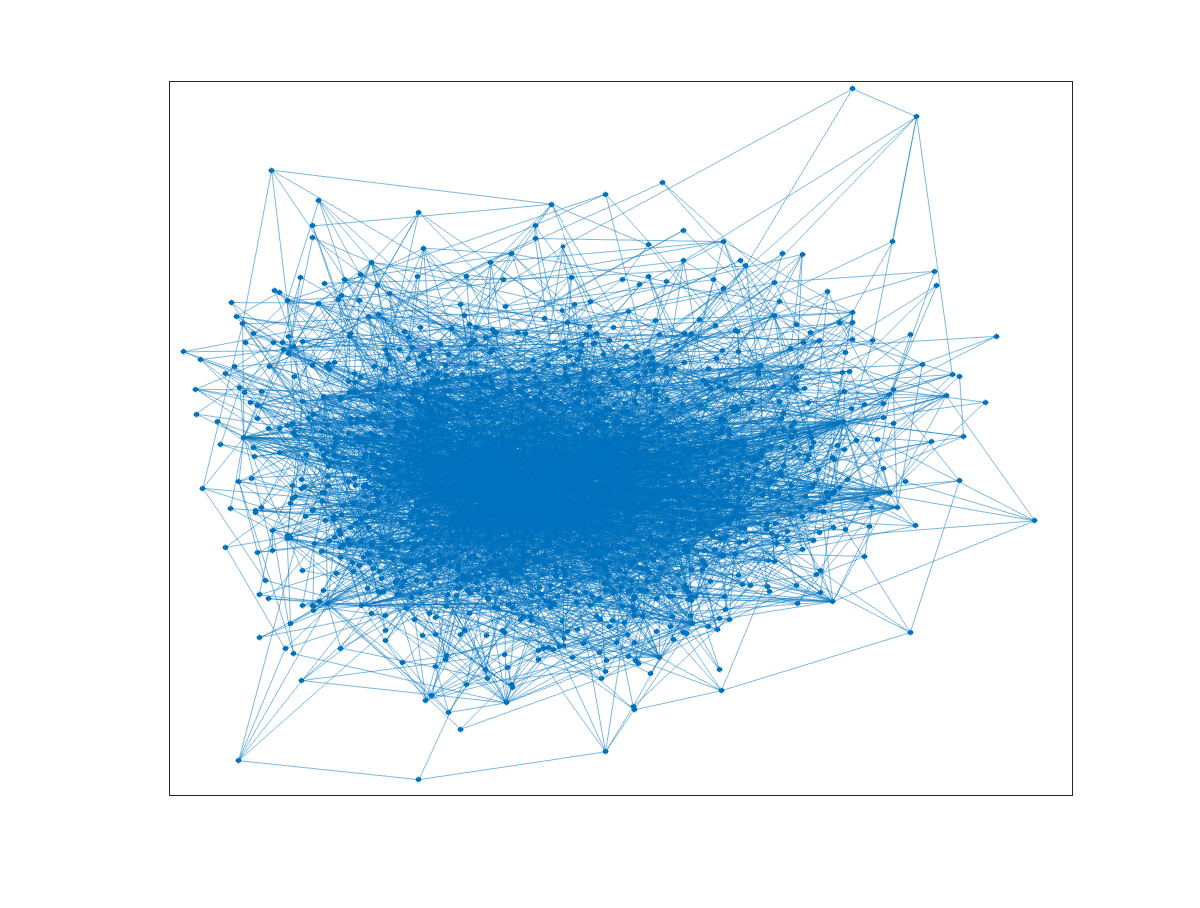
\includegraphics[width=3.5in]{network}
\caption{Large scale free network used for validation.}
\label{fig:network}
\end{figure}

\begin{figure}
\centering
%% Creator: Matplotlib, PGF backend
%%
%% To include the figure in your LaTeX document, write
%%   \input{<filename>.pgf}
%%
%% Make sure the required packages are loaded in your preamble
%%   \usepackage{pgf}
%%
%% Also ensure that all the required font packages are loaded; for instance,
%% the lmodern package is sometimes necessary when using math font.
%%   \usepackage{lmodern}
%%
%% Figures using additional raster images can only be included by \input if
%% they are in the same directory as the main LaTeX file. For loading figures
%% from other directories you can use the `import` package
%%   \usepackage{import}
%%
%% and then include the figures with
%%   \import{<path to file>}{<filename>.pgf}
%%
%% Matplotlib used the following preamble
%%   \def\mathdefault#1{#1}
%%   \everymath=\expandafter{\the\everymath\displaystyle}
%%   
%%   \usepackage{fontspec}
%%   \setmainfont{DejaVuSerif.ttf}[Path=\detokenize{/Users/billgoodwine/research/step/steps/lib/python3.11/site-packages/matplotlib/mpl-data/fonts/ttf/}]
%%   \setsansfont{DejaVuSans.ttf}[Path=\detokenize{/Users/billgoodwine/research/step/steps/lib/python3.11/site-packages/matplotlib/mpl-data/fonts/ttf/}]
%%   \setmonofont{DejaVuSansMono.ttf}[Path=\detokenize{/Users/billgoodwine/research/step/steps/lib/python3.11/site-packages/matplotlib/mpl-data/fonts/ttf/}]
%%   \makeatletter\@ifpackageloaded{underscore}{}{\usepackage[strings]{underscore}}\makeatother
%%
\begingroup%
\makeatletter%
\begin{pgfpicture}%
\pgfpathrectangle{\pgfpointorigin}{\pgfqpoint{3.500000in}{2.379431in}}%
\pgfusepath{use as bounding box, clip}%
\begin{pgfscope}%
\pgfsetbuttcap%
\pgfsetmiterjoin%
\definecolor{currentfill}{rgb}{1.000000,1.000000,1.000000}%
\pgfsetfillcolor{currentfill}%
\pgfsetlinewidth{0.000000pt}%
\definecolor{currentstroke}{rgb}{1.000000,1.000000,1.000000}%
\pgfsetstrokecolor{currentstroke}%
\pgfsetdash{}{0pt}%
\pgfpathmoveto{\pgfqpoint{0.000000in}{0.000000in}}%
\pgfpathlineto{\pgfqpoint{3.500000in}{0.000000in}}%
\pgfpathlineto{\pgfqpoint{3.500000in}{2.379431in}}%
\pgfpathlineto{\pgfqpoint{0.000000in}{2.379431in}}%
\pgfpathlineto{\pgfqpoint{0.000000in}{0.000000in}}%
\pgfpathclose%
\pgfusepath{fill}%
\end{pgfscope}%
\begin{pgfscope}%
\pgfsetbuttcap%
\pgfsetmiterjoin%
\definecolor{currentfill}{rgb}{1.000000,1.000000,1.000000}%
\pgfsetfillcolor{currentfill}%
\pgfsetlinewidth{0.000000pt}%
\definecolor{currentstroke}{rgb}{0.000000,0.000000,0.000000}%
\pgfsetstrokecolor{currentstroke}%
\pgfsetstrokeopacity{0.000000}%
\pgfsetdash{}{0pt}%
\pgfpathmoveto{\pgfqpoint{0.619136in}{0.571603in}}%
\pgfpathlineto{\pgfqpoint{3.350000in}{0.571603in}}%
\pgfpathlineto{\pgfqpoint{3.350000in}{2.229431in}}%
\pgfpathlineto{\pgfqpoint{0.619136in}{2.229431in}}%
\pgfpathlineto{\pgfqpoint{0.619136in}{0.571603in}}%
\pgfpathclose%
\pgfusepath{fill}%
\end{pgfscope}%
\begin{pgfscope}%
\pgfpathrectangle{\pgfqpoint{0.619136in}{0.571603in}}{\pgfqpoint{2.730864in}{1.657828in}}%
\pgfusepath{clip}%
\pgfsetrectcap%
\pgfsetroundjoin%
\pgfsetlinewidth{0.803000pt}%
\definecolor{currentstroke}{rgb}{0.690196,0.690196,0.690196}%
\pgfsetstrokecolor{currentstroke}%
\pgfsetdash{}{0pt}%
\pgfpathmoveto{\pgfqpoint{0.743267in}{0.571603in}}%
\pgfpathlineto{\pgfqpoint{0.743267in}{2.229431in}}%
\pgfusepath{stroke}%
\end{pgfscope}%
\begin{pgfscope}%
\pgfsetbuttcap%
\pgfsetroundjoin%
\definecolor{currentfill}{rgb}{0.000000,0.000000,0.000000}%
\pgfsetfillcolor{currentfill}%
\pgfsetlinewidth{0.803000pt}%
\definecolor{currentstroke}{rgb}{0.000000,0.000000,0.000000}%
\pgfsetstrokecolor{currentstroke}%
\pgfsetdash{}{0pt}%
\pgfsys@defobject{currentmarker}{\pgfqpoint{0.000000in}{-0.048611in}}{\pgfqpoint{0.000000in}{0.000000in}}{%
\pgfpathmoveto{\pgfqpoint{0.000000in}{0.000000in}}%
\pgfpathlineto{\pgfqpoint{0.000000in}{-0.048611in}}%
\pgfusepath{stroke,fill}%
}%
\begin{pgfscope}%
\pgfsys@transformshift{0.743267in}{0.571603in}%
\pgfsys@useobject{currentmarker}{}%
\end{pgfscope}%
\end{pgfscope}%
\begin{pgfscope}%
\definecolor{textcolor}{rgb}{0.000000,0.000000,0.000000}%
\pgfsetstrokecolor{textcolor}%
\pgfsetfillcolor{textcolor}%
\pgftext[x=0.743267in,y=0.474381in,,top]{\color{textcolor}{\rmfamily\fontsize{10.000000}{12.000000}\selectfont\catcode`\^=\active\def^{\ifmmode\sp\else\^{}\fi}\catcode`\%=\active\def%{\%}$\mathdefault{0}$}}%
\end{pgfscope}%
\begin{pgfscope}%
\pgfpathrectangle{\pgfqpoint{0.619136in}{0.571603in}}{\pgfqpoint{2.730864in}{1.657828in}}%
\pgfusepath{clip}%
\pgfsetrectcap%
\pgfsetroundjoin%
\pgfsetlinewidth{0.803000pt}%
\definecolor{currentstroke}{rgb}{0.690196,0.690196,0.690196}%
\pgfsetstrokecolor{currentstroke}%
\pgfsetdash{}{0pt}%
\pgfpathmoveto{\pgfqpoint{1.239787in}{0.571603in}}%
\pgfpathlineto{\pgfqpoint{1.239787in}{2.229431in}}%
\pgfusepath{stroke}%
\end{pgfscope}%
\begin{pgfscope}%
\pgfsetbuttcap%
\pgfsetroundjoin%
\definecolor{currentfill}{rgb}{0.000000,0.000000,0.000000}%
\pgfsetfillcolor{currentfill}%
\pgfsetlinewidth{0.803000pt}%
\definecolor{currentstroke}{rgb}{0.000000,0.000000,0.000000}%
\pgfsetstrokecolor{currentstroke}%
\pgfsetdash{}{0pt}%
\pgfsys@defobject{currentmarker}{\pgfqpoint{0.000000in}{-0.048611in}}{\pgfqpoint{0.000000in}{0.000000in}}{%
\pgfpathmoveto{\pgfqpoint{0.000000in}{0.000000in}}%
\pgfpathlineto{\pgfqpoint{0.000000in}{-0.048611in}}%
\pgfusepath{stroke,fill}%
}%
\begin{pgfscope}%
\pgfsys@transformshift{1.239787in}{0.571603in}%
\pgfsys@useobject{currentmarker}{}%
\end{pgfscope}%
\end{pgfscope}%
\begin{pgfscope}%
\definecolor{textcolor}{rgb}{0.000000,0.000000,0.000000}%
\pgfsetstrokecolor{textcolor}%
\pgfsetfillcolor{textcolor}%
\pgftext[x=1.239787in,y=0.474381in,,top]{\color{textcolor}{\rmfamily\fontsize{10.000000}{12.000000}\selectfont\catcode`\^=\active\def^{\ifmmode\sp\else\^{}\fi}\catcode`\%=\active\def%{\%}$\mathdefault{2}$}}%
\end{pgfscope}%
\begin{pgfscope}%
\pgfpathrectangle{\pgfqpoint{0.619136in}{0.571603in}}{\pgfqpoint{2.730864in}{1.657828in}}%
\pgfusepath{clip}%
\pgfsetrectcap%
\pgfsetroundjoin%
\pgfsetlinewidth{0.803000pt}%
\definecolor{currentstroke}{rgb}{0.690196,0.690196,0.690196}%
\pgfsetstrokecolor{currentstroke}%
\pgfsetdash{}{0pt}%
\pgfpathmoveto{\pgfqpoint{1.736308in}{0.571603in}}%
\pgfpathlineto{\pgfqpoint{1.736308in}{2.229431in}}%
\pgfusepath{stroke}%
\end{pgfscope}%
\begin{pgfscope}%
\pgfsetbuttcap%
\pgfsetroundjoin%
\definecolor{currentfill}{rgb}{0.000000,0.000000,0.000000}%
\pgfsetfillcolor{currentfill}%
\pgfsetlinewidth{0.803000pt}%
\definecolor{currentstroke}{rgb}{0.000000,0.000000,0.000000}%
\pgfsetstrokecolor{currentstroke}%
\pgfsetdash{}{0pt}%
\pgfsys@defobject{currentmarker}{\pgfqpoint{0.000000in}{-0.048611in}}{\pgfqpoint{0.000000in}{0.000000in}}{%
\pgfpathmoveto{\pgfqpoint{0.000000in}{0.000000in}}%
\pgfpathlineto{\pgfqpoint{0.000000in}{-0.048611in}}%
\pgfusepath{stroke,fill}%
}%
\begin{pgfscope}%
\pgfsys@transformshift{1.736308in}{0.571603in}%
\pgfsys@useobject{currentmarker}{}%
\end{pgfscope}%
\end{pgfscope}%
\begin{pgfscope}%
\definecolor{textcolor}{rgb}{0.000000,0.000000,0.000000}%
\pgfsetstrokecolor{textcolor}%
\pgfsetfillcolor{textcolor}%
\pgftext[x=1.736308in,y=0.474381in,,top]{\color{textcolor}{\rmfamily\fontsize{10.000000}{12.000000}\selectfont\catcode`\^=\active\def^{\ifmmode\sp\else\^{}\fi}\catcode`\%=\active\def%{\%}$\mathdefault{4}$}}%
\end{pgfscope}%
\begin{pgfscope}%
\pgfpathrectangle{\pgfqpoint{0.619136in}{0.571603in}}{\pgfqpoint{2.730864in}{1.657828in}}%
\pgfusepath{clip}%
\pgfsetrectcap%
\pgfsetroundjoin%
\pgfsetlinewidth{0.803000pt}%
\definecolor{currentstroke}{rgb}{0.690196,0.690196,0.690196}%
\pgfsetstrokecolor{currentstroke}%
\pgfsetdash{}{0pt}%
\pgfpathmoveto{\pgfqpoint{2.232829in}{0.571603in}}%
\pgfpathlineto{\pgfqpoint{2.232829in}{2.229431in}}%
\pgfusepath{stroke}%
\end{pgfscope}%
\begin{pgfscope}%
\pgfsetbuttcap%
\pgfsetroundjoin%
\definecolor{currentfill}{rgb}{0.000000,0.000000,0.000000}%
\pgfsetfillcolor{currentfill}%
\pgfsetlinewidth{0.803000pt}%
\definecolor{currentstroke}{rgb}{0.000000,0.000000,0.000000}%
\pgfsetstrokecolor{currentstroke}%
\pgfsetdash{}{0pt}%
\pgfsys@defobject{currentmarker}{\pgfqpoint{0.000000in}{-0.048611in}}{\pgfqpoint{0.000000in}{0.000000in}}{%
\pgfpathmoveto{\pgfqpoint{0.000000in}{0.000000in}}%
\pgfpathlineto{\pgfqpoint{0.000000in}{-0.048611in}}%
\pgfusepath{stroke,fill}%
}%
\begin{pgfscope}%
\pgfsys@transformshift{2.232829in}{0.571603in}%
\pgfsys@useobject{currentmarker}{}%
\end{pgfscope}%
\end{pgfscope}%
\begin{pgfscope}%
\definecolor{textcolor}{rgb}{0.000000,0.000000,0.000000}%
\pgfsetstrokecolor{textcolor}%
\pgfsetfillcolor{textcolor}%
\pgftext[x=2.232829in,y=0.474381in,,top]{\color{textcolor}{\rmfamily\fontsize{10.000000}{12.000000}\selectfont\catcode`\^=\active\def^{\ifmmode\sp\else\^{}\fi}\catcode`\%=\active\def%{\%}$\mathdefault{6}$}}%
\end{pgfscope}%
\begin{pgfscope}%
\pgfpathrectangle{\pgfqpoint{0.619136in}{0.571603in}}{\pgfqpoint{2.730864in}{1.657828in}}%
\pgfusepath{clip}%
\pgfsetrectcap%
\pgfsetroundjoin%
\pgfsetlinewidth{0.803000pt}%
\definecolor{currentstroke}{rgb}{0.690196,0.690196,0.690196}%
\pgfsetstrokecolor{currentstroke}%
\pgfsetdash{}{0pt}%
\pgfpathmoveto{\pgfqpoint{2.729349in}{0.571603in}}%
\pgfpathlineto{\pgfqpoint{2.729349in}{2.229431in}}%
\pgfusepath{stroke}%
\end{pgfscope}%
\begin{pgfscope}%
\pgfsetbuttcap%
\pgfsetroundjoin%
\definecolor{currentfill}{rgb}{0.000000,0.000000,0.000000}%
\pgfsetfillcolor{currentfill}%
\pgfsetlinewidth{0.803000pt}%
\definecolor{currentstroke}{rgb}{0.000000,0.000000,0.000000}%
\pgfsetstrokecolor{currentstroke}%
\pgfsetdash{}{0pt}%
\pgfsys@defobject{currentmarker}{\pgfqpoint{0.000000in}{-0.048611in}}{\pgfqpoint{0.000000in}{0.000000in}}{%
\pgfpathmoveto{\pgfqpoint{0.000000in}{0.000000in}}%
\pgfpathlineto{\pgfqpoint{0.000000in}{-0.048611in}}%
\pgfusepath{stroke,fill}%
}%
\begin{pgfscope}%
\pgfsys@transformshift{2.729349in}{0.571603in}%
\pgfsys@useobject{currentmarker}{}%
\end{pgfscope}%
\end{pgfscope}%
\begin{pgfscope}%
\definecolor{textcolor}{rgb}{0.000000,0.000000,0.000000}%
\pgfsetstrokecolor{textcolor}%
\pgfsetfillcolor{textcolor}%
\pgftext[x=2.729349in,y=0.474381in,,top]{\color{textcolor}{\rmfamily\fontsize{10.000000}{12.000000}\selectfont\catcode`\^=\active\def^{\ifmmode\sp\else\^{}\fi}\catcode`\%=\active\def%{\%}$\mathdefault{8}$}}%
\end{pgfscope}%
\begin{pgfscope}%
\pgfpathrectangle{\pgfqpoint{0.619136in}{0.571603in}}{\pgfqpoint{2.730864in}{1.657828in}}%
\pgfusepath{clip}%
\pgfsetrectcap%
\pgfsetroundjoin%
\pgfsetlinewidth{0.803000pt}%
\definecolor{currentstroke}{rgb}{0.690196,0.690196,0.690196}%
\pgfsetstrokecolor{currentstroke}%
\pgfsetdash{}{0pt}%
\pgfpathmoveto{\pgfqpoint{3.225870in}{0.571603in}}%
\pgfpathlineto{\pgfqpoint{3.225870in}{2.229431in}}%
\pgfusepath{stroke}%
\end{pgfscope}%
\begin{pgfscope}%
\pgfsetbuttcap%
\pgfsetroundjoin%
\definecolor{currentfill}{rgb}{0.000000,0.000000,0.000000}%
\pgfsetfillcolor{currentfill}%
\pgfsetlinewidth{0.803000pt}%
\definecolor{currentstroke}{rgb}{0.000000,0.000000,0.000000}%
\pgfsetstrokecolor{currentstroke}%
\pgfsetdash{}{0pt}%
\pgfsys@defobject{currentmarker}{\pgfqpoint{0.000000in}{-0.048611in}}{\pgfqpoint{0.000000in}{0.000000in}}{%
\pgfpathmoveto{\pgfqpoint{0.000000in}{0.000000in}}%
\pgfpathlineto{\pgfqpoint{0.000000in}{-0.048611in}}%
\pgfusepath{stroke,fill}%
}%
\begin{pgfscope}%
\pgfsys@transformshift{3.225870in}{0.571603in}%
\pgfsys@useobject{currentmarker}{}%
\end{pgfscope}%
\end{pgfscope}%
\begin{pgfscope}%
\definecolor{textcolor}{rgb}{0.000000,0.000000,0.000000}%
\pgfsetstrokecolor{textcolor}%
\pgfsetfillcolor{textcolor}%
\pgftext[x=3.225870in,y=0.474381in,,top]{\color{textcolor}{\rmfamily\fontsize{10.000000}{12.000000}\selectfont\catcode`\^=\active\def^{\ifmmode\sp\else\^{}\fi}\catcode`\%=\active\def%{\%}$\mathdefault{10}$}}%
\end{pgfscope}%
\begin{pgfscope}%
\definecolor{textcolor}{rgb}{0.000000,0.000000,0.000000}%
\pgfsetstrokecolor{textcolor}%
\pgfsetfillcolor{textcolor}%
\pgftext[x=1.984568in,y=0.284413in,,top]{\color{textcolor}{\rmfamily\fontsize{10.000000}{12.000000}\selectfont\catcode`\^=\active\def^{\ifmmode\sp\else\^{}\fi}\catcode`\%=\active\def%{\%}$t$}}%
\end{pgfscope}%
\begin{pgfscope}%
\pgfpathrectangle{\pgfqpoint{0.619136in}{0.571603in}}{\pgfqpoint{2.730864in}{1.657828in}}%
\pgfusepath{clip}%
\pgfsetrectcap%
\pgfsetroundjoin%
\pgfsetlinewidth{0.803000pt}%
\definecolor{currentstroke}{rgb}{0.690196,0.690196,0.690196}%
\pgfsetstrokecolor{currentstroke}%
\pgfsetdash{}{0pt}%
\pgfpathmoveto{\pgfqpoint{0.619136in}{0.646959in}}%
\pgfpathlineto{\pgfqpoint{3.350000in}{0.646959in}}%
\pgfusepath{stroke}%
\end{pgfscope}%
\begin{pgfscope}%
\pgfsetbuttcap%
\pgfsetroundjoin%
\definecolor{currentfill}{rgb}{0.000000,0.000000,0.000000}%
\pgfsetfillcolor{currentfill}%
\pgfsetlinewidth{0.803000pt}%
\definecolor{currentstroke}{rgb}{0.000000,0.000000,0.000000}%
\pgfsetstrokecolor{currentstroke}%
\pgfsetdash{}{0pt}%
\pgfsys@defobject{currentmarker}{\pgfqpoint{-0.048611in}{0.000000in}}{\pgfqpoint{-0.000000in}{0.000000in}}{%
\pgfpathmoveto{\pgfqpoint{-0.000000in}{0.000000in}}%
\pgfpathlineto{\pgfqpoint{-0.048611in}{0.000000in}}%
\pgfusepath{stroke,fill}%
}%
\begin{pgfscope}%
\pgfsys@transformshift{0.619136in}{0.646959in}%
\pgfsys@useobject{currentmarker}{}%
\end{pgfscope}%
\end{pgfscope}%
\begin{pgfscope}%
\definecolor{textcolor}{rgb}{0.000000,0.000000,0.000000}%
\pgfsetstrokecolor{textcolor}%
\pgfsetfillcolor{textcolor}%
\pgftext[x=0.344444in, y=0.594198in, left, base]{\color{textcolor}{\rmfamily\fontsize{10.000000}{12.000000}\selectfont\catcode`\^=\active\def^{\ifmmode\sp\else\^{}\fi}\catcode`\%=\active\def%{\%}$\mathdefault{0.0}$}}%
\end{pgfscope}%
\begin{pgfscope}%
\pgfpathrectangle{\pgfqpoint{0.619136in}{0.571603in}}{\pgfqpoint{2.730864in}{1.657828in}}%
\pgfusepath{clip}%
\pgfsetrectcap%
\pgfsetroundjoin%
\pgfsetlinewidth{0.803000pt}%
\definecolor{currentstroke}{rgb}{0.690196,0.690196,0.690196}%
\pgfsetstrokecolor{currentstroke}%
\pgfsetdash{}{0pt}%
\pgfpathmoveto{\pgfqpoint{0.619136in}{1.118566in}}%
\pgfpathlineto{\pgfqpoint{3.350000in}{1.118566in}}%
\pgfusepath{stroke}%
\end{pgfscope}%
\begin{pgfscope}%
\pgfsetbuttcap%
\pgfsetroundjoin%
\definecolor{currentfill}{rgb}{0.000000,0.000000,0.000000}%
\pgfsetfillcolor{currentfill}%
\pgfsetlinewidth{0.803000pt}%
\definecolor{currentstroke}{rgb}{0.000000,0.000000,0.000000}%
\pgfsetstrokecolor{currentstroke}%
\pgfsetdash{}{0pt}%
\pgfsys@defobject{currentmarker}{\pgfqpoint{-0.048611in}{0.000000in}}{\pgfqpoint{-0.000000in}{0.000000in}}{%
\pgfpathmoveto{\pgfqpoint{-0.000000in}{0.000000in}}%
\pgfpathlineto{\pgfqpoint{-0.048611in}{0.000000in}}%
\pgfusepath{stroke,fill}%
}%
\begin{pgfscope}%
\pgfsys@transformshift{0.619136in}{1.118566in}%
\pgfsys@useobject{currentmarker}{}%
\end{pgfscope}%
\end{pgfscope}%
\begin{pgfscope}%
\definecolor{textcolor}{rgb}{0.000000,0.000000,0.000000}%
\pgfsetstrokecolor{textcolor}%
\pgfsetfillcolor{textcolor}%
\pgftext[x=0.344444in, y=1.065804in, left, base]{\color{textcolor}{\rmfamily\fontsize{10.000000}{12.000000}\selectfont\catcode`\^=\active\def^{\ifmmode\sp\else\^{}\fi}\catcode`\%=\active\def%{\%}$\mathdefault{0.5}$}}%
\end{pgfscope}%
\begin{pgfscope}%
\pgfpathrectangle{\pgfqpoint{0.619136in}{0.571603in}}{\pgfqpoint{2.730864in}{1.657828in}}%
\pgfusepath{clip}%
\pgfsetrectcap%
\pgfsetroundjoin%
\pgfsetlinewidth{0.803000pt}%
\definecolor{currentstroke}{rgb}{0.690196,0.690196,0.690196}%
\pgfsetstrokecolor{currentstroke}%
\pgfsetdash{}{0pt}%
\pgfpathmoveto{\pgfqpoint{0.619136in}{1.590173in}}%
\pgfpathlineto{\pgfqpoint{3.350000in}{1.590173in}}%
\pgfusepath{stroke}%
\end{pgfscope}%
\begin{pgfscope}%
\pgfsetbuttcap%
\pgfsetroundjoin%
\definecolor{currentfill}{rgb}{0.000000,0.000000,0.000000}%
\pgfsetfillcolor{currentfill}%
\pgfsetlinewidth{0.803000pt}%
\definecolor{currentstroke}{rgb}{0.000000,0.000000,0.000000}%
\pgfsetstrokecolor{currentstroke}%
\pgfsetdash{}{0pt}%
\pgfsys@defobject{currentmarker}{\pgfqpoint{-0.048611in}{0.000000in}}{\pgfqpoint{-0.000000in}{0.000000in}}{%
\pgfpathmoveto{\pgfqpoint{-0.000000in}{0.000000in}}%
\pgfpathlineto{\pgfqpoint{-0.048611in}{0.000000in}}%
\pgfusepath{stroke,fill}%
}%
\begin{pgfscope}%
\pgfsys@transformshift{0.619136in}{1.590173in}%
\pgfsys@useobject{currentmarker}{}%
\end{pgfscope}%
\end{pgfscope}%
\begin{pgfscope}%
\definecolor{textcolor}{rgb}{0.000000,0.000000,0.000000}%
\pgfsetstrokecolor{textcolor}%
\pgfsetfillcolor{textcolor}%
\pgftext[x=0.344444in, y=1.537411in, left, base]{\color{textcolor}{\rmfamily\fontsize{10.000000}{12.000000}\selectfont\catcode`\^=\active\def^{\ifmmode\sp\else\^{}\fi}\catcode`\%=\active\def%{\%}$\mathdefault{1.0}$}}%
\end{pgfscope}%
\begin{pgfscope}%
\pgfpathrectangle{\pgfqpoint{0.619136in}{0.571603in}}{\pgfqpoint{2.730864in}{1.657828in}}%
\pgfusepath{clip}%
\pgfsetrectcap%
\pgfsetroundjoin%
\pgfsetlinewidth{0.803000pt}%
\definecolor{currentstroke}{rgb}{0.690196,0.690196,0.690196}%
\pgfsetstrokecolor{currentstroke}%
\pgfsetdash{}{0pt}%
\pgfpathmoveto{\pgfqpoint{0.619136in}{2.061779in}}%
\pgfpathlineto{\pgfqpoint{3.350000in}{2.061779in}}%
\pgfusepath{stroke}%
\end{pgfscope}%
\begin{pgfscope}%
\pgfsetbuttcap%
\pgfsetroundjoin%
\definecolor{currentfill}{rgb}{0.000000,0.000000,0.000000}%
\pgfsetfillcolor{currentfill}%
\pgfsetlinewidth{0.803000pt}%
\definecolor{currentstroke}{rgb}{0.000000,0.000000,0.000000}%
\pgfsetstrokecolor{currentstroke}%
\pgfsetdash{}{0pt}%
\pgfsys@defobject{currentmarker}{\pgfqpoint{-0.048611in}{0.000000in}}{\pgfqpoint{-0.000000in}{0.000000in}}{%
\pgfpathmoveto{\pgfqpoint{-0.000000in}{0.000000in}}%
\pgfpathlineto{\pgfqpoint{-0.048611in}{0.000000in}}%
\pgfusepath{stroke,fill}%
}%
\begin{pgfscope}%
\pgfsys@transformshift{0.619136in}{2.061779in}%
\pgfsys@useobject{currentmarker}{}%
\end{pgfscope}%
\end{pgfscope}%
\begin{pgfscope}%
\definecolor{textcolor}{rgb}{0.000000,0.000000,0.000000}%
\pgfsetstrokecolor{textcolor}%
\pgfsetfillcolor{textcolor}%
\pgftext[x=0.344444in, y=2.009018in, left, base]{\color{textcolor}{\rmfamily\fontsize{10.000000}{12.000000}\selectfont\catcode`\^=\active\def^{\ifmmode\sp\else\^{}\fi}\catcode`\%=\active\def%{\%}$\mathdefault{1.5}$}}%
\end{pgfscope}%
\begin{pgfscope}%
\definecolor{textcolor}{rgb}{0.000000,0.000000,0.000000}%
\pgfsetstrokecolor{textcolor}%
\pgfsetfillcolor{textcolor}%
\pgftext[x=0.288889in,y=1.400517in,,bottom,rotate=90.000000]{\color{textcolor}{\rmfamily\fontsize{10.000000}{12.000000}\selectfont\catcode`\^=\active\def^{\ifmmode\sp\else\^{}\fi}\catcode`\%=\active\def%{\%}$x(t)$}}%
\end{pgfscope}%
\begin{pgfscope}%
\pgfpathrectangle{\pgfqpoint{0.619136in}{0.571603in}}{\pgfqpoint{2.730864in}{1.657828in}}%
\pgfusepath{clip}%
\pgfsetrectcap%
\pgfsetroundjoin%
\pgfsetlinewidth{1.505625pt}%
\definecolor{currentstroke}{rgb}{0.121569,0.466667,0.705882}%
\pgfsetstrokecolor{currentstroke}%
\pgfsetdash{}{0pt}%
\pgfpathmoveto{\pgfqpoint{0.743267in}{0.646959in}}%
\pgfpathlineto{\pgfqpoint{0.768093in}{0.682386in}}%
\pgfpathlineto{\pgfqpoint{0.792919in}{0.780125in}}%
\pgfpathlineto{\pgfqpoint{0.817745in}{0.927346in}}%
\pgfpathlineto{\pgfqpoint{0.842571in}{1.105687in}}%
\pgfpathlineto{\pgfqpoint{0.867397in}{1.303178in}}%
\pgfpathlineto{\pgfqpoint{0.892223in}{1.502849in}}%
\pgfpathlineto{\pgfqpoint{0.917049in}{1.691695in}}%
\pgfpathlineto{\pgfqpoint{0.941875in}{1.857514in}}%
\pgfpathlineto{\pgfqpoint{0.966701in}{1.991365in}}%
\pgfpathlineto{\pgfqpoint{0.991527in}{2.086977in}}%
\pgfpathlineto{\pgfqpoint{1.016353in}{2.141168in}}%
\pgfpathlineto{\pgfqpoint{1.041179in}{2.154075in}}%
\pgfpathlineto{\pgfqpoint{1.066005in}{2.128256in}}%
\pgfpathlineto{\pgfqpoint{1.090831in}{2.068916in}}%
\pgfpathlineto{\pgfqpoint{1.115657in}{1.982902in}}%
\pgfpathlineto{\pgfqpoint{1.140483in}{1.878273in}}%
\pgfpathlineto{\pgfqpoint{1.165309in}{1.763675in}}%
\pgfpathlineto{\pgfqpoint{1.190135in}{1.647580in}}%
\pgfpathlineto{\pgfqpoint{1.214961in}{1.537900in}}%
\pgfpathlineto{\pgfqpoint{1.239787in}{1.441369in}}%
\pgfpathlineto{\pgfqpoint{1.264613in}{1.363268in}}%
\pgfpathlineto{\pgfqpoint{1.289439in}{1.307208in}}%
\pgfpathlineto{\pgfqpoint{1.314265in}{1.274963in}}%
\pgfpathlineto{\pgfqpoint{1.339091in}{1.266612in}}%
\pgfpathlineto{\pgfqpoint{1.363917in}{1.280601in}}%
\pgfpathlineto{\pgfqpoint{1.388743in}{1.314023in}}%
\pgfpathlineto{\pgfqpoint{1.413569in}{1.362952in}}%
\pgfpathlineto{\pgfqpoint{1.438395in}{1.422739in}}%
\pgfpathlineto{\pgfqpoint{1.463222in}{1.488445in}}%
\pgfpathlineto{\pgfqpoint{1.488048in}{1.555164in}}%
\pgfpathlineto{\pgfqpoint{1.512874in}{1.618339in}}%
\pgfpathlineto{\pgfqpoint{1.537700in}{1.674077in}}%
\pgfpathlineto{\pgfqpoint{1.562526in}{1.719301in}}%
\pgfpathlineto{\pgfqpoint{1.587352in}{1.751915in}}%
\pgfpathlineto{\pgfqpoint{1.612178in}{1.770858in}}%
\pgfpathlineto{\pgfqpoint{1.637004in}{1.776057in}}%
\pgfpathlineto{\pgfqpoint{1.661830in}{1.768381in}}%
\pgfpathlineto{\pgfqpoint{1.686656in}{1.749474in}}%
\pgfpathlineto{\pgfqpoint{1.711482in}{1.721582in}}%
\pgfpathlineto{\pgfqpoint{1.736308in}{1.687365in}}%
\pgfpathlineto{\pgfqpoint{1.761134in}{1.649659in}}%
\pgfpathlineto{\pgfqpoint{1.785960in}{1.611290in}}%
\pgfpathlineto{\pgfqpoint{1.810786in}{1.574883in}}%
\pgfpathlineto{\pgfqpoint{1.835612in}{1.542690in}}%
\pgfpathlineto{\pgfqpoint{1.860438in}{1.516497in}}%
\pgfpathlineto{\pgfqpoint{1.885264in}{1.497523in}}%
\pgfpathlineto{\pgfqpoint{1.910090in}{1.486399in}}%
\pgfpathlineto{\pgfqpoint{1.934916in}{1.483182in}}%
\pgfpathlineto{\pgfqpoint{1.959742in}{1.487387in}}%
\pgfpathlineto{\pgfqpoint{1.984568in}{1.498083in}}%
\pgfpathlineto{\pgfqpoint{2.009394in}{1.513986in}}%
\pgfpathlineto{\pgfqpoint{2.034220in}{1.533573in}}%
\pgfpathlineto{\pgfqpoint{2.059046in}{1.555216in}}%
\pgfpathlineto{\pgfqpoint{2.083872in}{1.577287in}}%
\pgfpathlineto{\pgfqpoint{2.108698in}{1.598274in}}%
\pgfpathlineto{\pgfqpoint{2.133524in}{1.616872in}}%
\pgfpathlineto{\pgfqpoint{2.158350in}{1.632049in}}%
\pgfpathlineto{\pgfqpoint{2.183176in}{1.643092in}}%
\pgfpathlineto{\pgfqpoint{2.208002in}{1.649628in}}%
\pgfpathlineto{\pgfqpoint{2.232829in}{1.651615in}}%
\pgfpathlineto{\pgfqpoint{2.257655in}{1.649323in}}%
\pgfpathlineto{\pgfqpoint{2.282481in}{1.643281in}}%
\pgfpathlineto{\pgfqpoint{2.307307in}{1.634220in}}%
\pgfpathlineto{\pgfqpoint{2.332133in}{1.623014in}}%
\pgfpathlineto{\pgfqpoint{2.356959in}{1.610598in}}%
\pgfpathlineto{\pgfqpoint{2.381785in}{1.597908in}}%
\pgfpathlineto{\pgfqpoint{2.406611in}{1.585816in}}%
\pgfpathlineto{\pgfqpoint{2.431437in}{1.575076in}}%
\pgfpathlineto{\pgfqpoint{2.456263in}{1.566288in}}%
\pgfpathlineto{\pgfqpoint{2.481089in}{1.559866in}}%
\pgfpathlineto{\pgfqpoint{2.505915in}{1.556032in}}%
\pgfpathlineto{\pgfqpoint{2.530741in}{1.554813in}}%
\pgfpathlineto{\pgfqpoint{2.555567in}{1.556062in}}%
\pgfpathlineto{\pgfqpoint{2.580393in}{1.559478in}}%
\pgfpathlineto{\pgfqpoint{2.605219in}{1.564642in}}%
\pgfpathlineto{\pgfqpoint{2.630045in}{1.571056in}}%
\pgfpathlineto{\pgfqpoint{2.654871in}{1.578181in}}%
\pgfpathlineto{\pgfqpoint{2.679697in}{1.585480in}}%
\pgfpathlineto{\pgfqpoint{2.704523in}{1.592449in}}%
\pgfpathlineto{\pgfqpoint{2.729349in}{1.598653in}}%
\pgfpathlineto{\pgfqpoint{2.754175in}{1.603744in}}%
\pgfpathlineto{\pgfqpoint{2.779001in}{1.607480in}}%
\pgfpathlineto{\pgfqpoint{2.803827in}{1.609731in}}%
\pgfpathlineto{\pgfqpoint{2.828653in}{1.610477in}}%
\pgfpathlineto{\pgfqpoint{2.853479in}{1.609801in}}%
\pgfpathlineto{\pgfqpoint{2.878305in}{1.607873in}}%
\pgfpathlineto{\pgfqpoint{2.903131in}{1.604931in}}%
\pgfpathlineto{\pgfqpoint{2.927957in}{1.601263in}}%
\pgfpathlineto{\pgfqpoint{2.952783in}{1.597175in}}%
\pgfpathlineto{\pgfqpoint{2.977610in}{1.592979in}}%
\pgfpathlineto{\pgfqpoint{3.002436in}{1.588964in}}%
\pgfpathlineto{\pgfqpoint{3.027262in}{1.585382in}}%
\pgfpathlineto{\pgfqpoint{3.052088in}{1.582435in}}%
\pgfpathlineto{\pgfqpoint{3.076914in}{1.580263in}}%
\pgfpathlineto{\pgfqpoint{3.101740in}{1.578944in}}%
\pgfpathlineto{\pgfqpoint{3.126566in}{1.578490in}}%
\pgfpathlineto{\pgfqpoint{3.151392in}{1.578855in}}%
\pgfpathlineto{\pgfqpoint{3.176218in}{1.579944in}}%
\pgfpathlineto{\pgfqpoint{3.201044in}{1.581620in}}%
\pgfpathlineto{\pgfqpoint{3.225870in}{1.583719in}}%
\pgfusepath{stroke}%
\end{pgfscope}%
\begin{pgfscope}%
\pgfsetrectcap%
\pgfsetmiterjoin%
\pgfsetlinewidth{0.803000pt}%
\definecolor{currentstroke}{rgb}{0.000000,0.000000,0.000000}%
\pgfsetstrokecolor{currentstroke}%
\pgfsetdash{}{0pt}%
\pgfpathmoveto{\pgfqpoint{0.619136in}{0.571603in}}%
\pgfpathlineto{\pgfqpoint{0.619136in}{2.229431in}}%
\pgfusepath{stroke}%
\end{pgfscope}%
\begin{pgfscope}%
\pgfsetrectcap%
\pgfsetmiterjoin%
\pgfsetlinewidth{0.803000pt}%
\definecolor{currentstroke}{rgb}{0.000000,0.000000,0.000000}%
\pgfsetstrokecolor{currentstroke}%
\pgfsetdash{}{0pt}%
\pgfpathmoveto{\pgfqpoint{3.350000in}{0.571603in}}%
\pgfpathlineto{\pgfqpoint{3.350000in}{2.229431in}}%
\pgfusepath{stroke}%
\end{pgfscope}%
\begin{pgfscope}%
\pgfsetrectcap%
\pgfsetmiterjoin%
\pgfsetlinewidth{0.803000pt}%
\definecolor{currentstroke}{rgb}{0.000000,0.000000,0.000000}%
\pgfsetstrokecolor{currentstroke}%
\pgfsetdash{}{0pt}%
\pgfpathmoveto{\pgfqpoint{0.619136in}{0.571603in}}%
\pgfpathlineto{\pgfqpoint{3.350000in}{0.571603in}}%
\pgfusepath{stroke}%
\end{pgfscope}%
\begin{pgfscope}%
\pgfsetrectcap%
\pgfsetmiterjoin%
\pgfsetlinewidth{0.803000pt}%
\definecolor{currentstroke}{rgb}{0.000000,0.000000,0.000000}%
\pgfsetstrokecolor{currentstroke}%
\pgfsetdash{}{0pt}%
\pgfpathmoveto{\pgfqpoint{0.619136in}{2.229431in}}%
\pgfpathlineto{\pgfqpoint{3.350000in}{2.229431in}}%
\pgfusepath{stroke}%
\end{pgfscope}%
\end{pgfpicture}%
\makeatother%
\endgroup%

\vspace*{-5pt}
\caption{Response of scale free network.}
\label{fig:sfresp}
\end{figure}

Because it is a mechanical system with 2000 nodes, the overall system has
extremely high order dynamics. The purpose of the research outlined in the
references is to determine reduced order models and determine when a fractional
order ``reduced order'' model better matches the response than a standard second
order model. Using two different optimization methods (Matlab
\texttt{patternsearch} (deterministic) and \texttt{particleswarm} (stochastic))
the best fit of a fractional order unit step response and second order step
response were determined. 

We then compare the order determined by the optimization method, which is very
slow, to the order predicted by the neural network, which is very fast.  The
predicted order by the neural network was 1.782. The predicted order by the two
optimization methods was 1.784, showing nearly exact agreement.


\section{CONCLUSIONS}
\label{sec:conclusions}

A conclusion section is not required. Although a conclusion may review the main
points of the paper, do not replicate the abstract as the conclusion. A
conclusion might elaborate on the importance of the work or suggest applications
and extensions. 

%\addtolength{\textheight}{-12cm} 

\bibliographystyle{IEEEtran}
\bibliography{references,goodwine}

\end{document}
